\RequirePackage{etoolbox}
\csdef{input@path}{%
 {sty/}% 
 {figures/}%
}%

\documentclass{article}

\title{Probability, illustrated}
\author{Alexandre Bouchard-C\^ot\'e}
\date{}

\usepackage{textcomp,mathrsfs}
\usepackage{graphicx,amssymb,amsmath,amsthm,mathrsfs}
\usepackage{multirow,makeidx,algorithmic,algorithm}
\usepackage{latexsym,graphicx,amssymb,amsmath,amsthm,mathrsfs}
\usepackage{mathrsfs}
\usepackage{amssymb}
\usepackage{booktabs,fancyhdr} 
\usepackage{rotating}
\usepackage{pdflscape}
\usepackage{graphicx}
\usepackage{array}
\usepackage{bigints}
\usepackage{listings}
\usepackage{titlesec}
\usepackage{mathtools}
\usepackage{amsthm}
\usepackage{amsmath}
\usepackage{natbib}
\usepackage{caption}
\usepackage{subcaption}

% links inside a doc
\usepackage{hyperref}
\hypersetup{colorlinks,citecolor=blue,urlcolor=blue,filecolor=blue,backref=page}

% for notation and abbreviations (links and tables)
\usepackage{notation}

% for internal use (comments etc)
\newcounter{xxx}
\setcounter{xxx}{0}
\newcommand\XXX[1]{{\bf \em \addtocounter{xxx}{1} (\thexxx) [[#1]]}}






% \makeatletter%
% \newcommand\exercise[2]{% 
%   \expandafter\newcommand\csname #2\endcsname{%
%     \processabbreviation{#1}{#2}{#3}{}%
%   }%
%   \expandafter\newcommand\csname #2s\endcsname{%
%     \processabbreviation{#1}{#2}{#3}{s}%
%   }%
% }%
% \newcommand\processabbreviation[4]{%
%   \ifcsname checkifdefined#2\endcsname% Already defined: create a link, and use the abbreviation
%       {\protect\hyperlink{#2}{\color{black}{#2#4}}}%
%     \else% First occurrence:
%       {\protect\Hy@raisedlink{\protect\hypertarget{#2}{}}{#3 (#2#4)}}% Create a target
%       \expandafter\gdef\csname checkifdefined#2\endcsname{1}% Remember it was encountered
%       \def\temp{#1}\ifx\temp\empty%
%         \relax%
%       \else%
%         \nomenclature{#2}{#1}%
%       \fi%
%     \fi%
% }%
% \makeatother% 
% dot product
\newcommand\dotprod[2]{\langle #1, #2\rangle}  

% reals
\newcommand\R{{\mathbb R}} 
\newcommand\Z{{\mathbb Z}} 
\newcommand\G{{\mathbb G}}       

% probability relatex
\renewcommand\P{{\mathbb P}}        
\newcommand\E{{\mathbb E}}        % expectation 
\def\1{{\mathbf 1}}        % indicator (need def b/c of non-alpha macro)
\newcommand\var{{\text {\bf Var}}}    % variance
\renewcommand\L{\mathbf L}

% binomial distribution
\DeclareMathOperator{\Bin}{Bin}
\DeclareMathOperator{\Poi}{Poi}
\DeclareMathOperator{\Bern}{Bern}
\DeclareMathOperator{\PP}{PP}
\DeclareMathOperator{\Unif}{Unif}

\newcommand{\ev}{\text{ ev.}}
\newcommand{\io}{\text{ i.o.}}

% big O
\renewcommand\O{\mathcal{O}}

% \int f(x) \ud x
\newcommand{\ud}{\,\mathrm{d}}    

% conditional defs
\newcommand\bracearraycond[1]{\left\{ \begin{array}{ll} #1 \end{array} \right.}

% define equal
\newcommand\defeq{\coloneqq}


% support
\DeclareMathOperator{\support}{support}
\DeclareMathOperator{\argmin}{argmin}

% maps to with name
\newcommand\labelledmapsto[1]{\stackrel{#1}{\longmapsto}}

% distributed according to unnormalized density
\newcommand\simpropto{\stackrel{\propto}{\sim}}

\def\ascv{\stackrel{\scriptscriptstyle a.s.}{\longrightarrow}}     % almost sure convergnece
\def\pcv{\stackrel{\scriptscriptstyle \P}{\longrightarrow}}        % convergence in P
\def\ltcv{\stackrel{\scriptscriptstyle\L^2}{\longrightarrow}}      % L2 convergnece
\def\lpcv{\stackrel{\scriptscriptstyle\L^p}{\longrightarrow}}      % Lp convergnece
\def\dcv{\stackrel{\scriptscriptstyle d}{\longrightarrow}}         % convergence in d
\def\deq{\stackrel{\scriptscriptstyle d}{=}}         % equal in d
\def\iidsim{\stackrel{\scriptscriptstyle \textrm{iid}}{\sim}}         % iid


% abbreviations
\abbreviation{CTMC}{Continuous Time Markov Chains}
\abbreviation{CDF}{Cumulative Distribution Function}
\abbreviation{PMF}{Probability mass function}

% terminology
\terminology{reversible}{reversible}
\terminology{sigmaalg}{$\sigma$-algebra}

%%%% conventions %%%%
% vectors: suffix V, e.g. dV, zV, etc
% densities: prefix f, followed by variable(s) or description, eg. fwxy, femi, etc
% probability mass function: prefix p, same rule as density otherwise
% conditioning: use the letter 'l' in the macro, eg. pdlQ for p_{d|Q}

% overwritten constants
\let\oldOmega\Omega
\let\oldsqcup\sqcup

% time/phylogeny notation
\notation*[Sample space]{Omega}{\oldOmega}
\notation[A $\sigma$-algebra (closed collection of events)]{events}{{\mathcal F}}
\notation[A collection of events that do not necessarily form a $\sigma$-algebra (a potentially ``broken'' collection of events)]{generators}{{\mathcal S}}
\notation[The Borel $\sigma$-algebra]{borels}{{\mathcal F}_\text{B}}
\notation[A set of states]{states}{{\mathcal X}}
\notation*[Disjoint union]{sqcup}{\oldsqcup}



% use to create table of symbols
\makenomenclature

\begin{document}

\maketitle
\noindent\hrulefill
\vspace{0.5in}
\begin{center}
	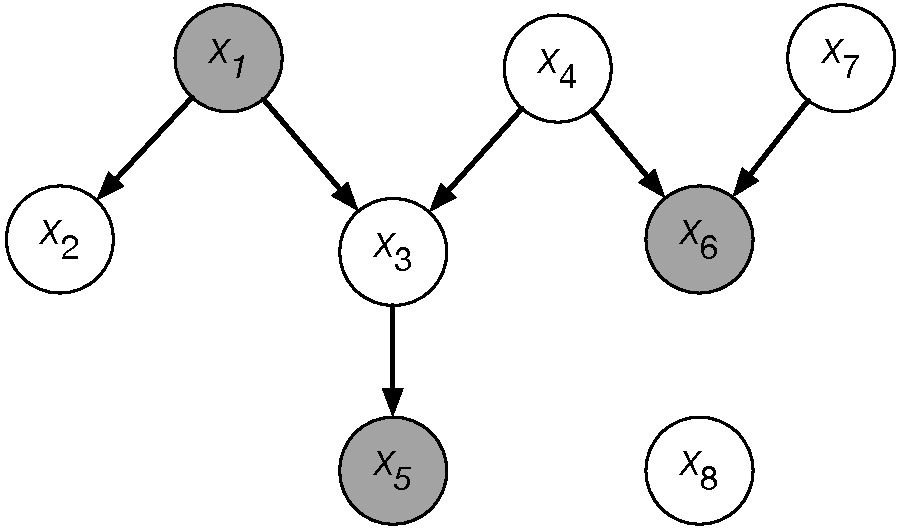
\includegraphics[width=0.8\linewidth]{figures/graph-model-cond}
\end{center}
\vspace{0.5in}
\noindent\hrulefill
 \vspace{1.8in} 



\noindent\begin{minipage}{0.3\textwidth}% adapt widths of minipages to your needs
	
\includegraphics[width=\linewidth]{figures/logo}
\end{minipage}%
\hfill%
\begin{minipage}{0.6\textwidth}\raggedright
	This work is licensed under a Creative Commons Attribution 4.0 International License.
\end{minipage}


\newpage

\noindent\hrulefill
\tableofcontents
\noindent\hrulefill



\newpage


\section{Motivations}

\point{Why learn probability theory?} 
\begin{enumerate}
	\item Probability theory is a fundamental tool in statistics, computer science, physics, econometrics, and many more traditionally quantitative fields. It is also quickly gaining in importance in fields making the quantitative transition, for example biology, linguistics, sociology, and many more. 
	\item The theory is beautiful in its own right. Probability Theory can also be approached as a branch of pure mathematics. 
\end{enumerate}
 
Both of the above points are excellent motivations. However by the nature of this course (we are in a stats department!), I will focus on the first point above and heavily use practical motivations throughout the notes. 

Why is probability a fundamental tool in so many fields? Because Probability Theory is useful for creating \emph{models}. 

\point{Models} are sketches of reality that capture the essential of a problem while being amenable to mathematical analysis. Probability-based models are great at incorporating phenomena like uncertainty and non-linearity. Moreover, compared to other types of models you might be familiar with (e.g. linear algebra or calculus based), they arguable tend to be more resilient to \emph{mis-specification}, i.e. they can recover from certain mismatches between the model and reality (data) in the sense of still giving good predictions.

There are many other motivations. I will just mention two more quickly:

\point{From model to prediction:} in Bayesian statistics, probability theory is essential not only to formulate models, but also to make predictions. Bayesian statisticians construct a probability model in which both the known quantities (data) and the unknown quantities are modelled using random variables. In Bayesian inference, prediction then involves  conditioning on the data.  We will use Bayesian statistics as a recurrent example when talking about conditioning. 

\point{The computational power of randomness.}  Probability Theory arises in a surprising way in the subfields of computer science concerned with the design and analysis of algorithms. Researchers have found since the 1940s many problems where the best way to solve deterministic problems is to introduce artificial randomness in the execution of the algorithm (an idea called \emph{algorithmic randomness}). Consider for example the problem of quickly approximating the volume of an arbitrary convex body. In a 1991 landmark paper \cite{dyer_random_1991}, Dyer, Frieze and Kanna devised the first provably efficient approximation algorithm, which crucially depends on algorithmic randomness to perform random walks. Moreover, it is known that no efficient deterministic algorithms can provide accurate approximations \cite{bfirfiny_computing_nodate}. There are many instances where there are no known deterministic algorithms and where algorithmic randomness is necessary to scale to large problems.  


\section{Foundations}

\point{On being formal:}  An important thing to realize is that despite the fact that Probability Theory is used to model uncertainty, it is as formal as any other fields of mathematics (despite what you may have been led to believe if you took a course using the standard undergraduate way of teaching). Formalization of the field was achieved by Kolmogorov in the 1930s, when he realized that the same tools used to formalize the notions of area and volume (measures) could be applied to probabilities. 

\point{On intuition:} While being formal is useful, intuition is important too. Probability is very connected to the real world so using your intuition is also very useful in making guesses that you can then prove using theory.

\point{Why measure theory?} Measure theory is the standard framework used to formalize probability theory. There are several reasons to learn the basics of measure theory (i.e., as Pollard puts it, to be \emph{user} of measure theory). We will see some of these technical motivations as we go along: 
\begin{enumerate}
	\item Unified treatment of things are taught separately in naive undergraduate probability course: discrete/continuous, univariate/multivariate. 
	\item Certain results about expectations are easier to state and hold more generally under the measure-theoretic definition of expectations.
	\item Establishing independence can in certain case be much easier under the measure theoretic definition of independence.
\end{enumerate}
However in my view the main motivation is that a big chunk of the literature is written in the language of measure theory. This course will prepare you so that you can be fearless when reading the stat literature. 

The danger is to be too formal and that the notation gets in the way of the intuition. I will avoid this pitfall. I will also skip the tedious details that I find less useful in statistics, e.g. certain proofs of existence, especially if they do not reveal a technique more broadly applicable 


\subsection{The basic vocabulary of probability}

The axioms of probability, formulated by Kolmogorov in the 1930s, provide a vocabulary and basic set of rules used in everything that follows. We look at how they become alive by showing how they are used to build two simple models (the second, not as simple as it initially looks!).

\point{Recurrent example:} imagine an infinite railroad, modelled by the integers $\Z = \{\dots, -3, -2, -1, 0, 1, 2, 3, \dots\}$. A train starts at position zero. At every time step,the train operator flips a coin. If the coin shows heads, the train moves left by one unit. Otherwise, the train moves to the right by one unit. 

We will look at two versions of this example, version A, where there is fuel limit which restricts the train to six moves, and version B, where there is no fuel limit. 

Let us start with version A. 

\point{Outcomes/scenarios:} several scenarios can arise from the dice-driven train ``story'' or ``experiment''. For example the train could go left, right, left, right, right, left. Or it could go left, right, right, right, right, left. We will call these two scenarios, two \emph{outcomes}. The usual letter for one outcome is $\omega$ or $s$. 

To help visualization, we will draw one outcome in the time series example as a graph where the x-axis is time $t$ and the y-axis is the position at time $t$. Here is one example for version A:
\begin{center}
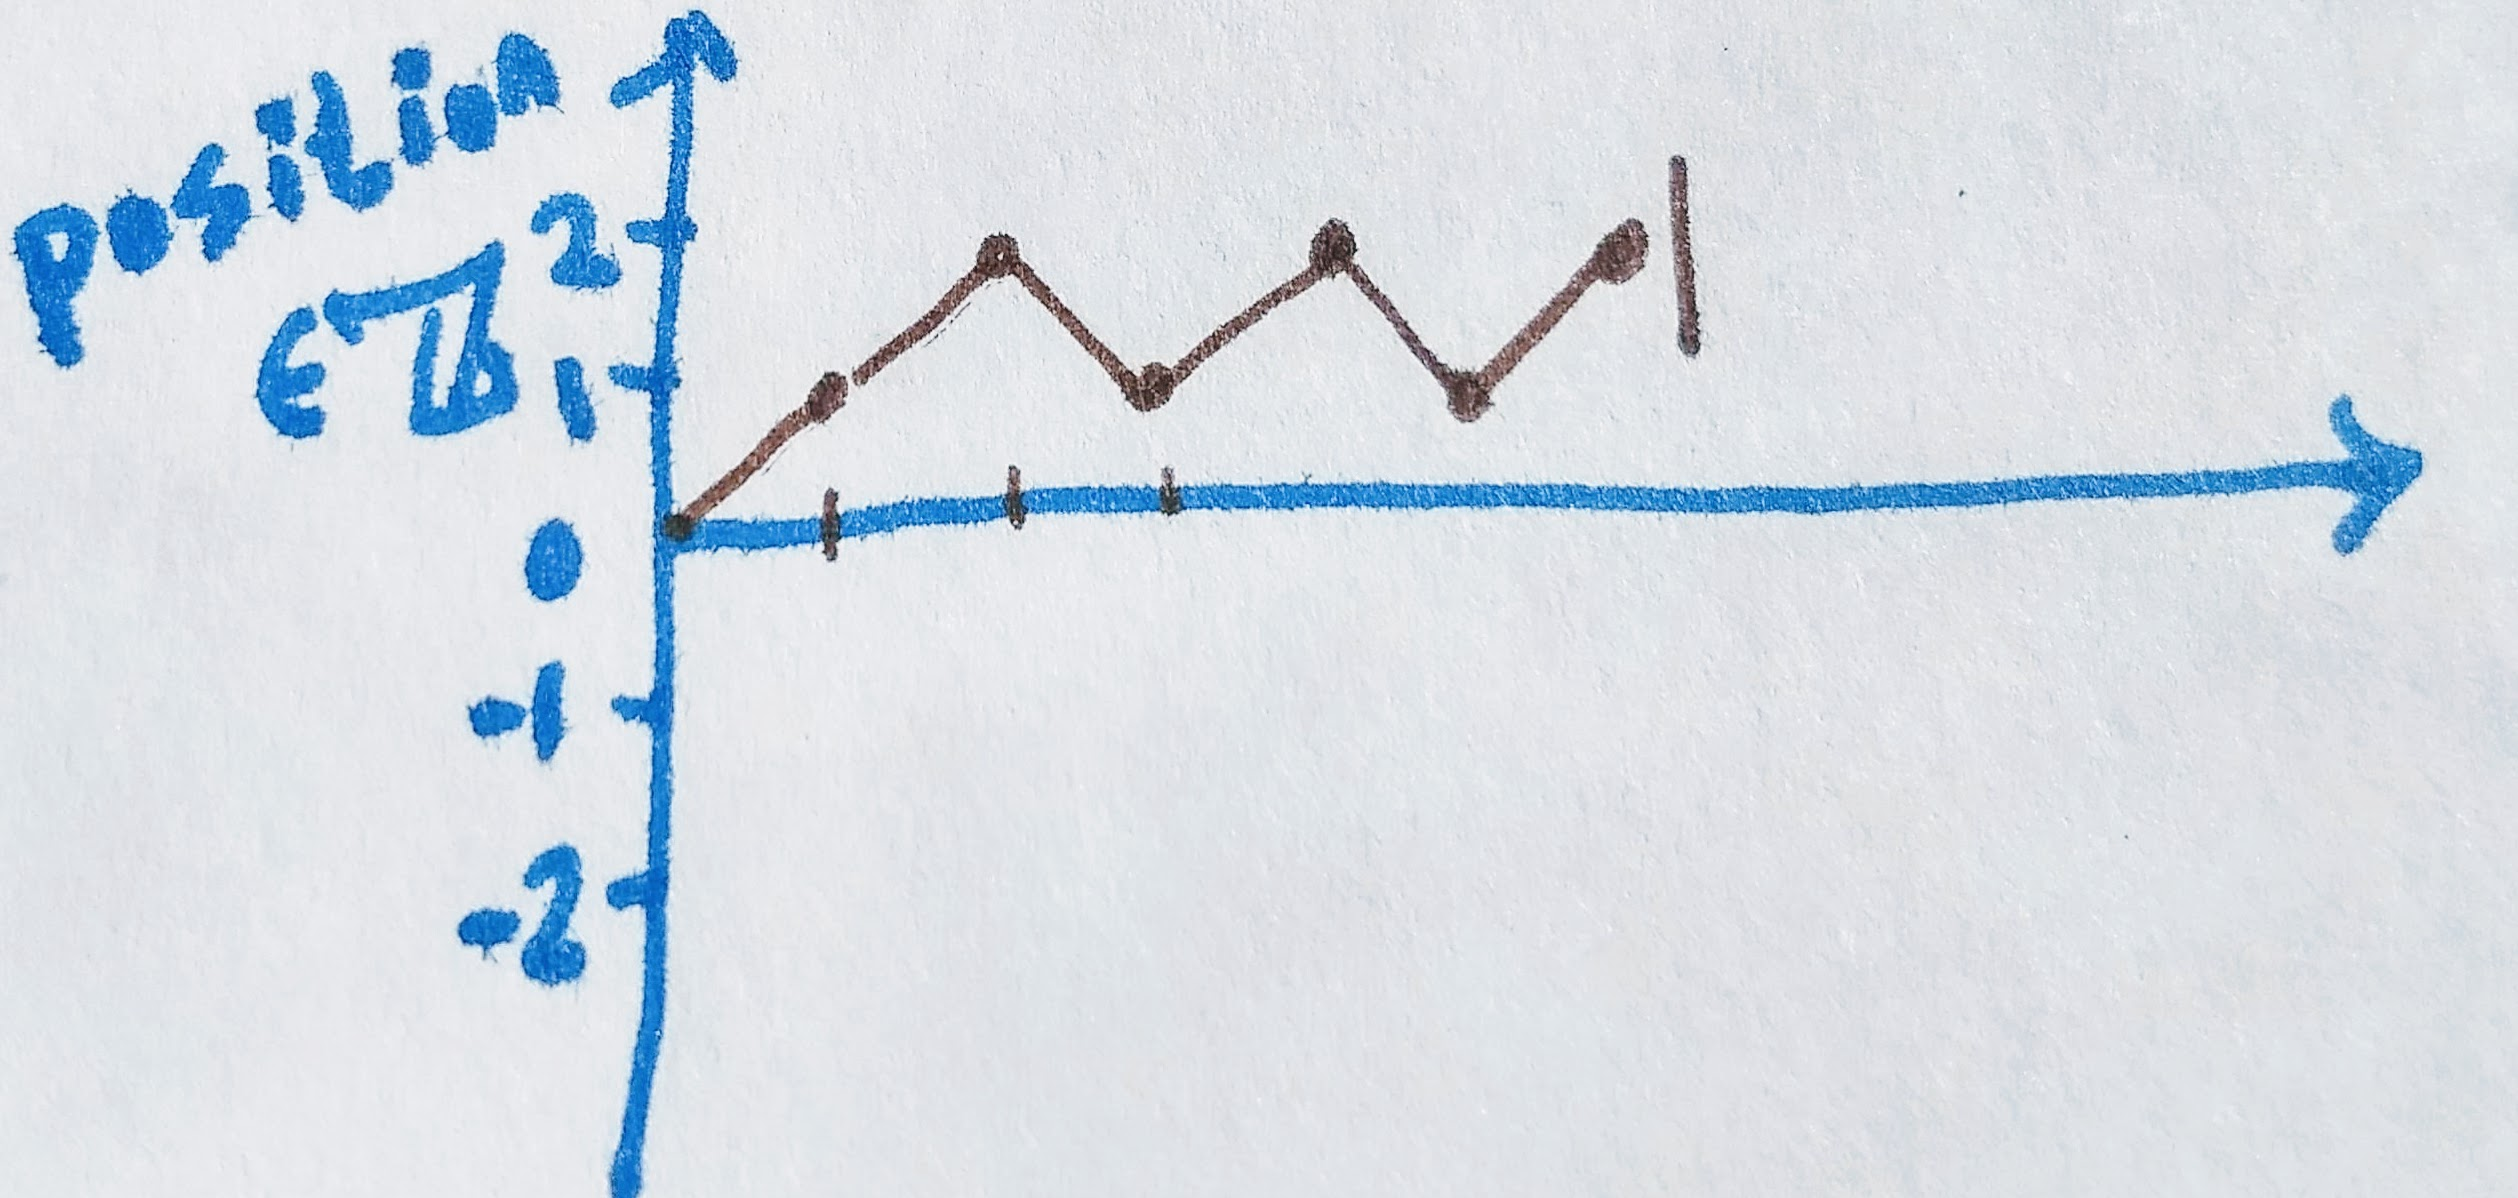
\includegraphics[width=0.5\linewidth]{figures/train1}
\end{center}
and for version B (infinite fuel):
\begin{center}
	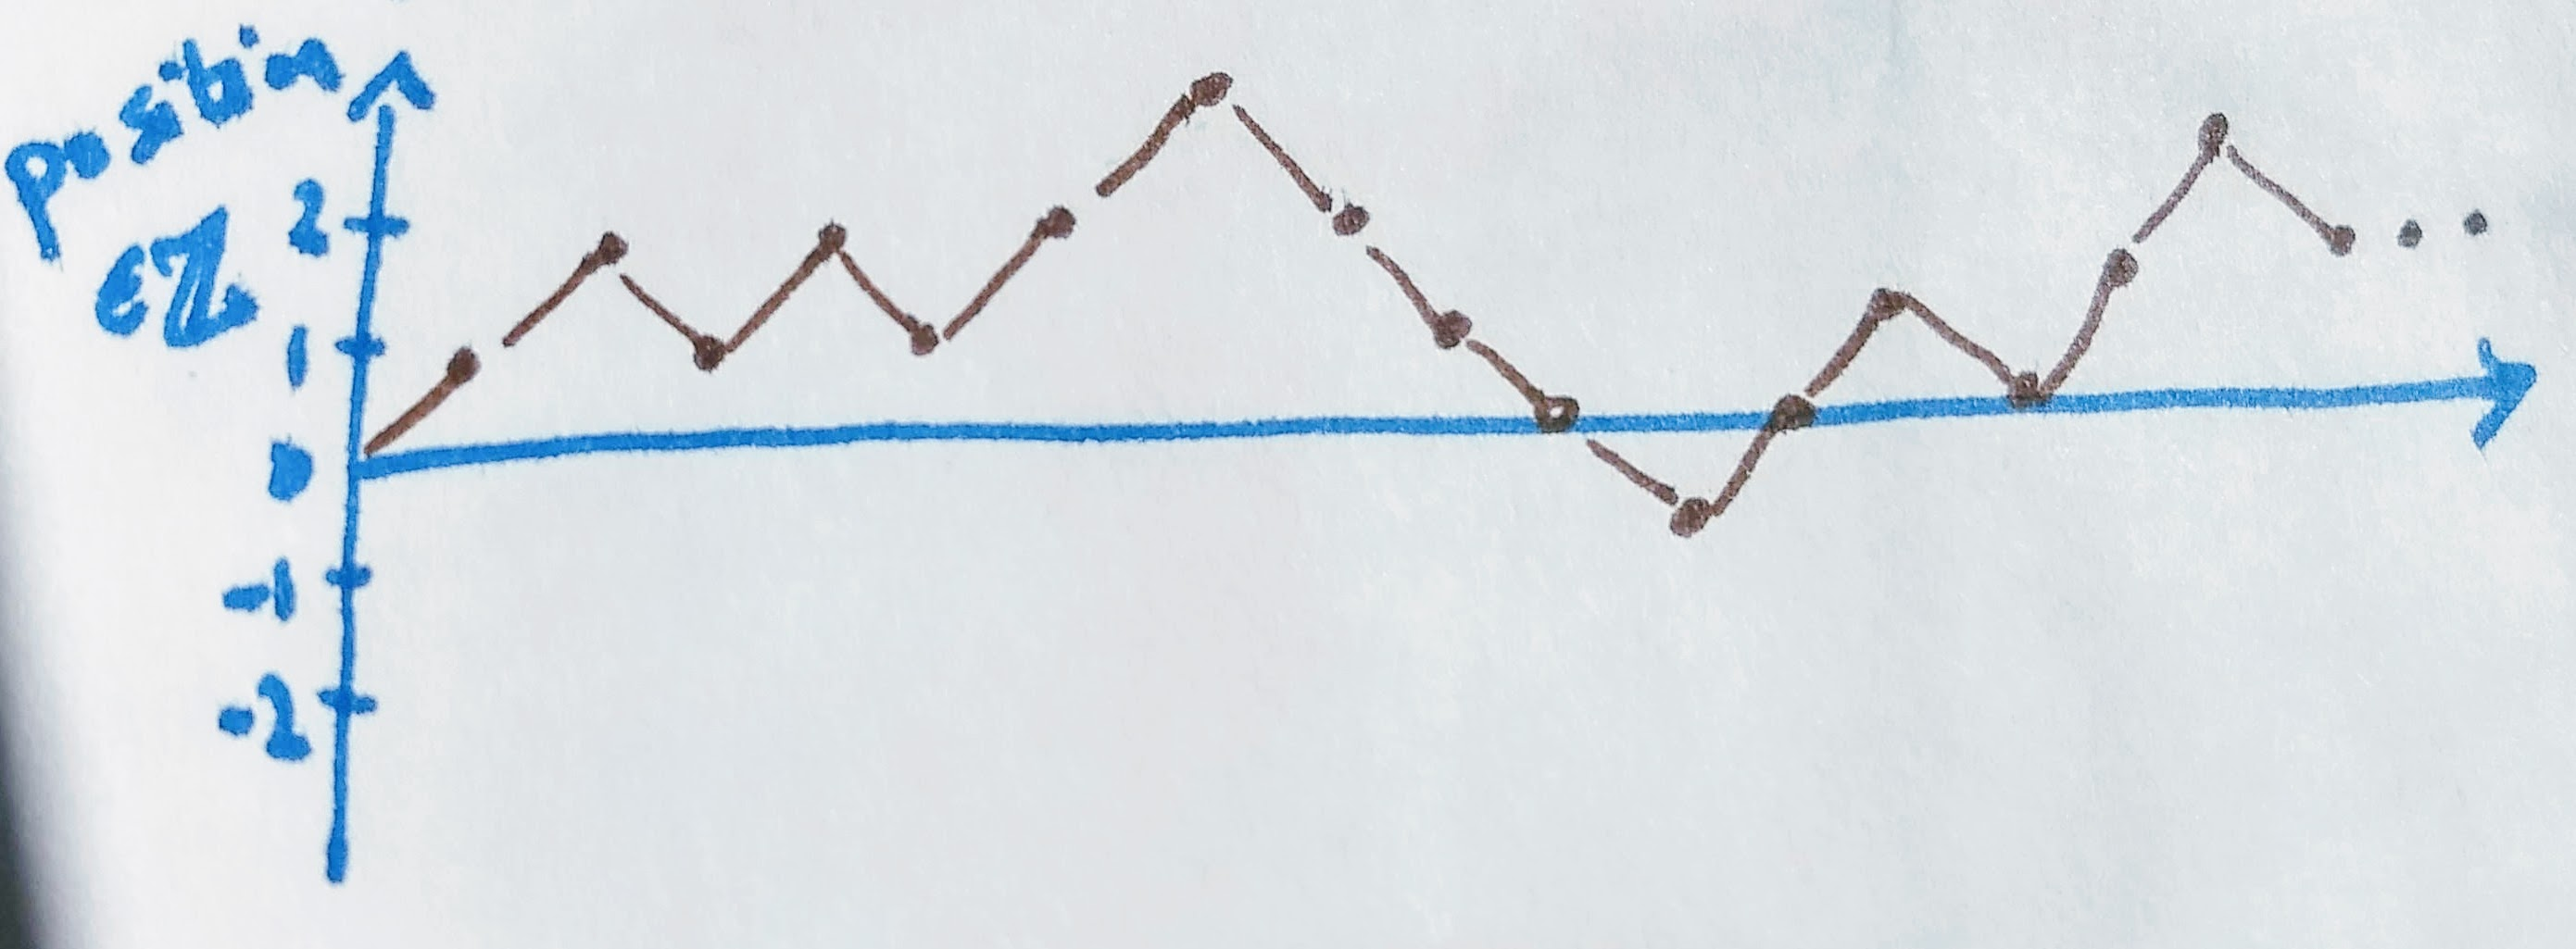
\includegraphics[width=0.5\linewidth]{figures/train2}
\end{center}

\point{Definition:} The set of all possible outcomes is called the \emph{sample space}, which I will denote by $\Omega$ or $S$. 

\point{Example:} what is the size or cardinality of $\Omega$ (i.e. the number of elements in it) for version A of our train example? I will denote the size by $|\Omega|$. Answer:$2^6$ because there are six bits each free to take two possible values. We conclude that the probability of any given outcome in version A is $1/64$. Note that 
\[ \sum_{\omega \in \Omega} \text{probability of outcome $\omega$} = 1. \]
Here is a picture for the train version A example:
\begin{center}
	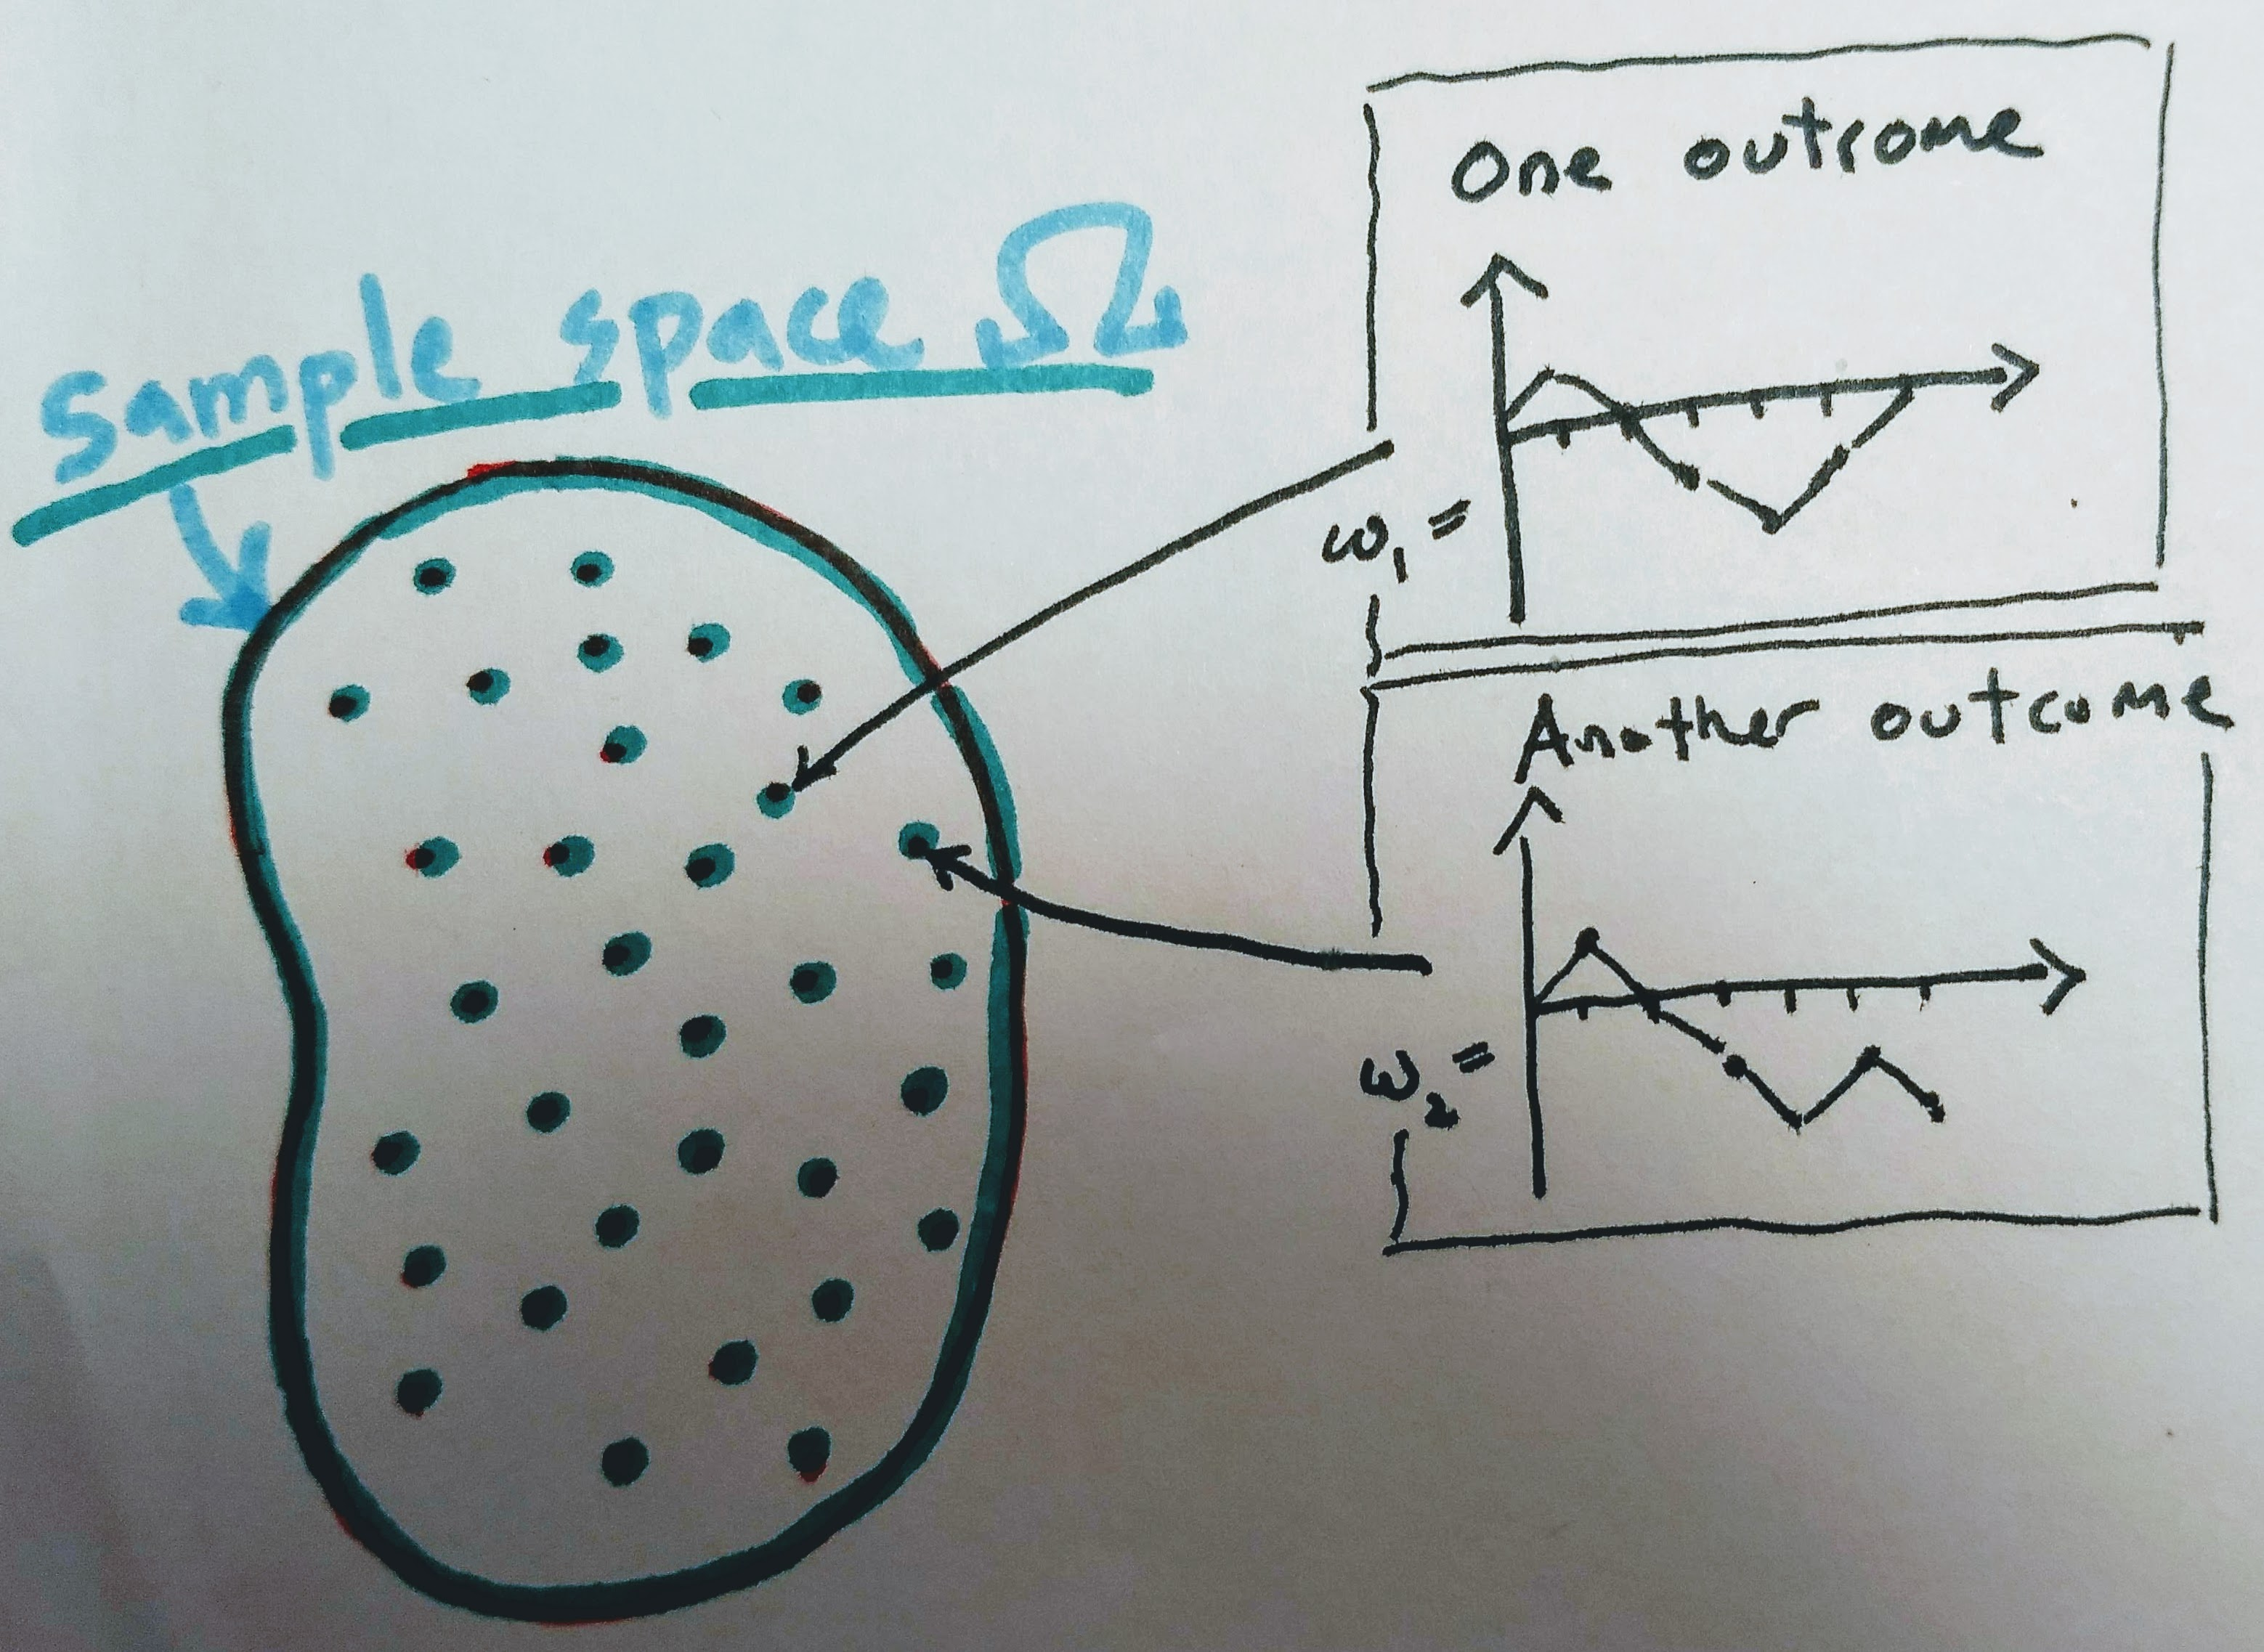
\includegraphics[width=0.5\linewidth]{figures/outcomes}
\end{center}

\point{Science-fiction interpretation:} if you read or watch science fiction (e.g. check out ``The man in the High Castle'' by Philip K. Dick), you may think about an outcome as encoding all the information for one universe, and the the set of all outcomes (the sample space) as the \emph{multiverse}. 

\point{Note:} an outcome may contain many bits of information. We only need one of those bits to get two different outcomes. I.e. outcomes can be very similar, but not identical. 

\point{Definition:} a set of outcomes is called an \emph{event}.

\point{Example:} events are often created using a property defining what outcomes are in the event. For example, consider the set of outcomes where the train goes left in the second time step, $A_1$. We use the terminology ``the event that the train goes left in the second time step.''  What is its size? Notice that events that are described by a small number of properties tend to be large, while event that are described by a larger number of properties tend to be smaller. 
\begin{center}
	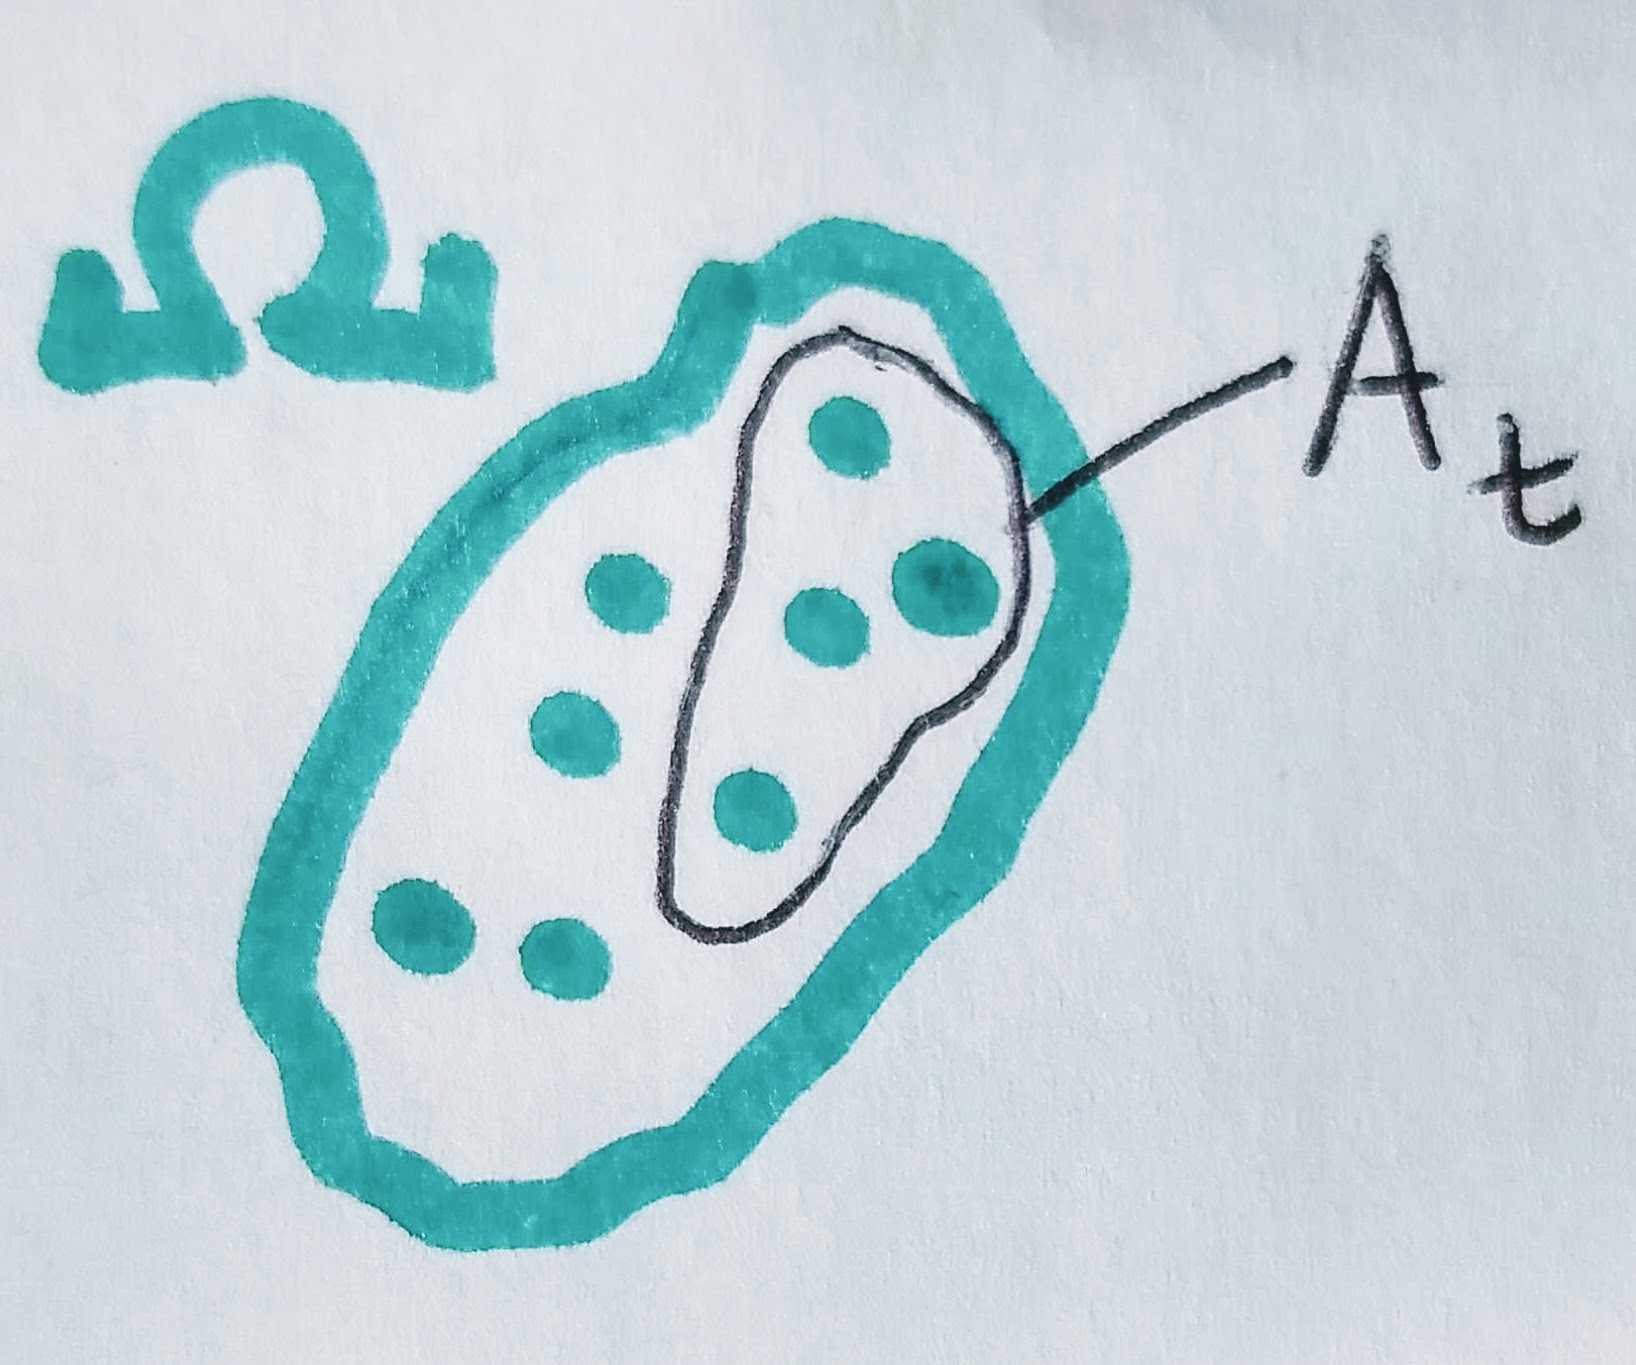
\includegraphics[width=0.3\linewidth]{figures/event}
\end{center}

\point{Partitions:} often we consider not one event but several events at once. For example we want to categorize outcomes into sub-cases. This can be done using partitions. A \emph{partition} of a set $E$ (for example $E = \Omega$), is a collection\footnote{Just a synonym for set.} of events $B_1, B_2, \dots$ such that (1) $B_i \cap B_j = \emptyset$ for all $i \neq j$ and (2) $\cup B_i = E$. Each $B_i$ is called a block.

\point{Decision trees} are useful to organize a hierarchy of events. Each node in the tree is an event. At the root, we put $\Omega$. When $|\Omega| < \infty$, at the leave we have \emph{singletons}, i.e. sets with only one element. In between, each node of the tree is split into subcases. More formally, say we are at a node corresponding to event $E$. Pick a \emph{partition} $B_1, B_2, \dots$ is of $E$. Then the children of $E$ in the decision tree are defined as the blocks of the partition splitting $E$.
\begin{center}
	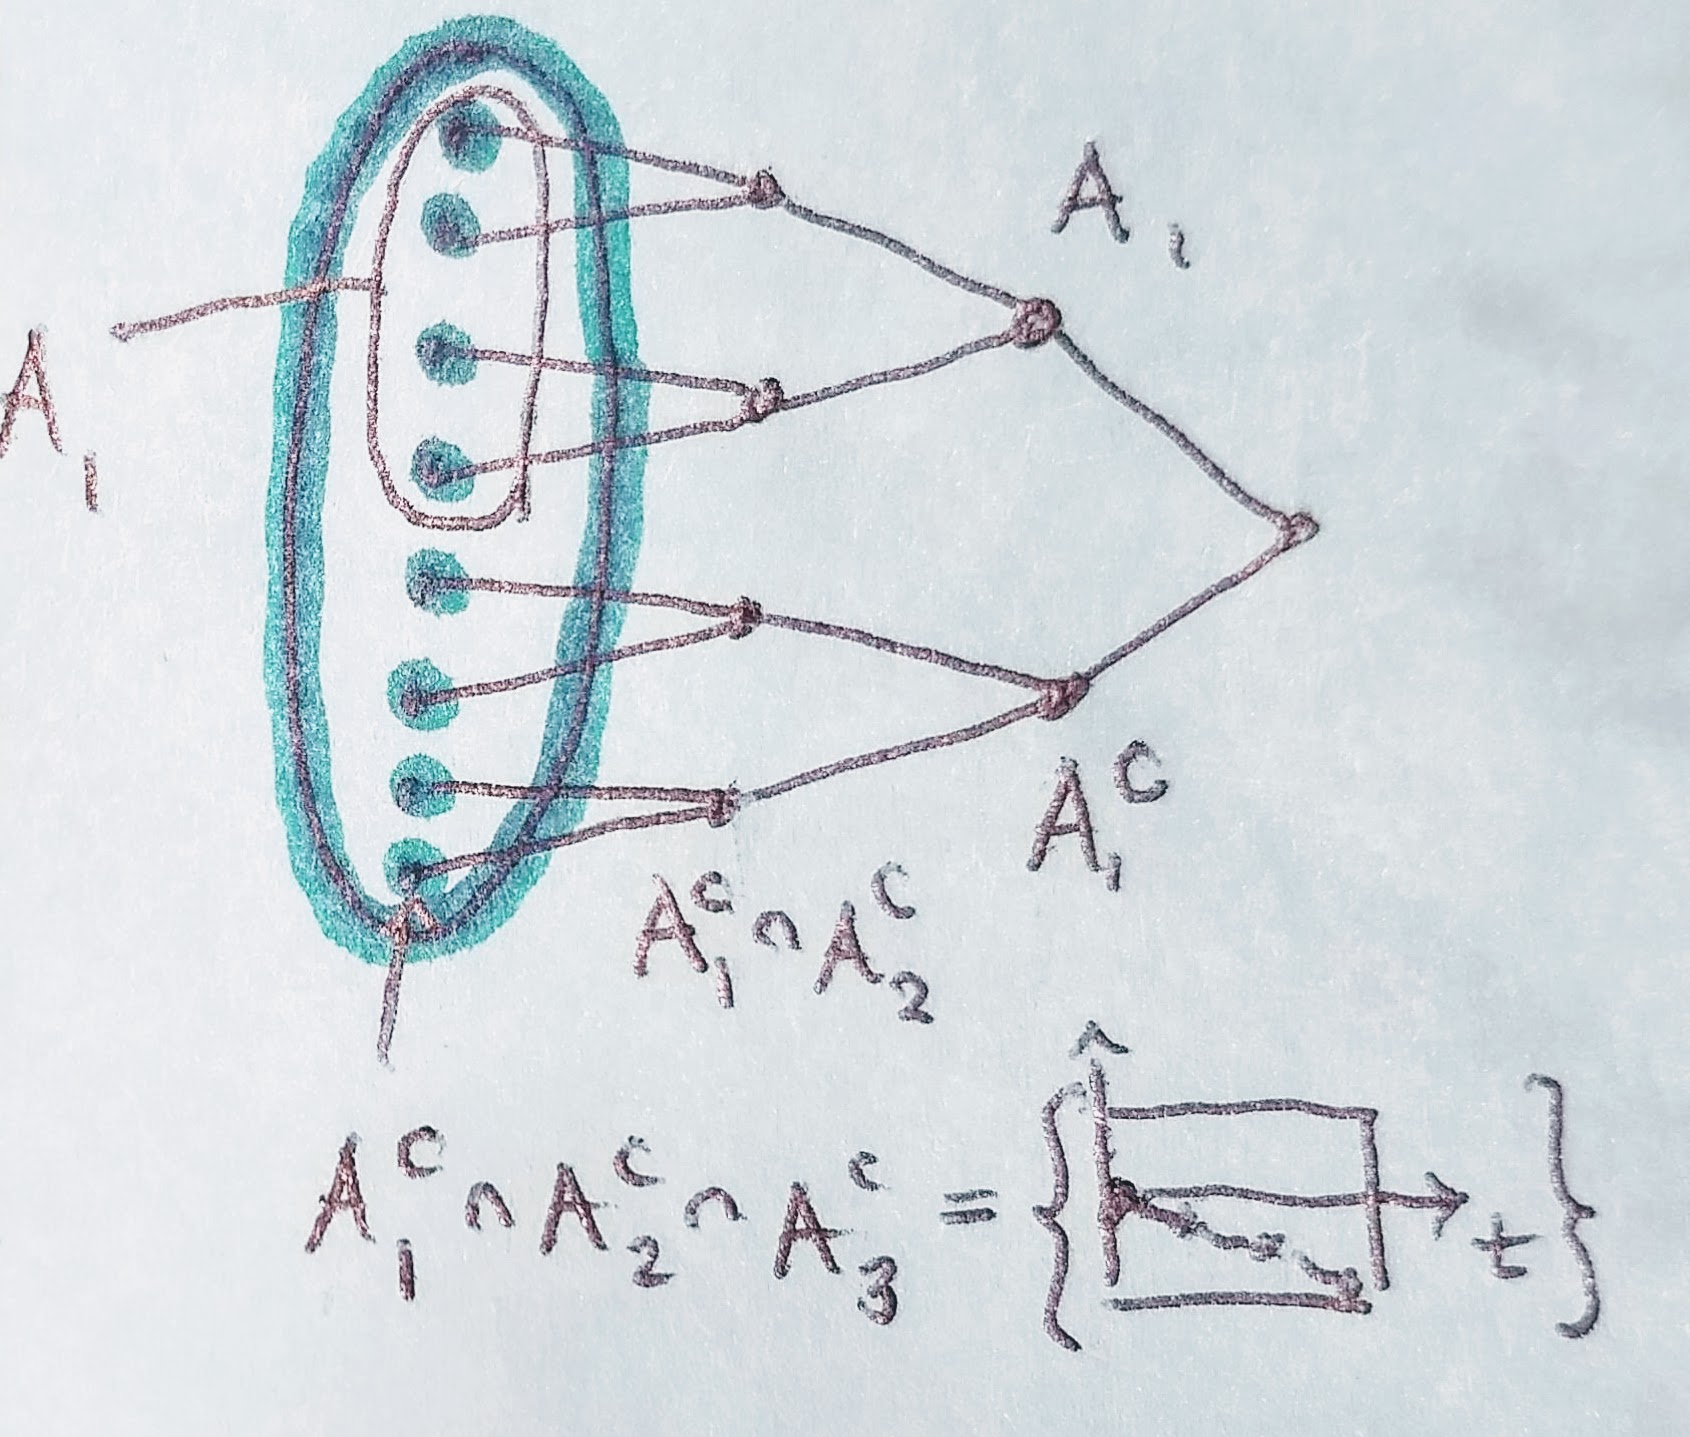
\includegraphics[width=0.5\linewidth]{figures/decision-tree}
\end{center}

\point{Additivity:} it is not too hard to see in example A that the probability of \emph{disjoint} events (i.e. non-intersecting events) can be added up. E.g.:
\begin{align*} 
&\text{probability go left in first turn} + \text{probability go right in first two turns} \\ 
&= \text{probability go left in first turn or right in first two turns}. 
\end{align*} 
Both sides are equal to $1/2 + 1/4$.

\point{Note:} it is not too hard to see in example A that the probability of \emph{overlapping} events (i.e. intersecting events) cannot always be added up. E.g.:
\begin{align*} 
	&\text{probability go left in first turn} + \text{probability go left in first two turns} \\
	&\neq \text{probability go left in first turn or left in first two turns}.
\end{align*}
The left hand side is equal to $1/2 + 1/4$ while the right hand side is equal to $1/2$. 

\point{A routine task} in probability problems consists in expressing events of unknown probability in terms of events of known probability. 

\point{Exercise/example:} express, in version A of the train example, the event that the train eventually returns home (position zero), in terms of the events: 
\[ A_t = \text{event that the train goes left in the $t$-th time step},\]
which have known probability. Do it using only the set theoretic operations $\cup$, $\cap$, and set complement $A_t^\complement$.


\subsection{Motivating the axioms of probability}

\point{Difficulty pre-Kolmogorov/pre-1930s:} people were already very good at doing computations for things like version A of the train. But surprisingly, they were running into serious foundational problems when trying to formalize the theory for version B of the problem!

\point{Difficulty:} in version B, we cannot always define probability of events by adding up probability of individual outcomes. We cannot have these three things:
\begin{align*}
	\text{probability of one path} &= \lim_{t \to \infty} (1/2)^t = 0 \\
	\text{probability of $\Omega$} &= 1 \\
	\sum_{\omega \in \Omega} \text{probability of outcome $\omega$} &= \text{probability of $\Omega$}.
\end{align*}
The problem is that each individually appears to make sense (the third one, in the light of the disjoint additivity observation), but they are inconsistent! We will see that the third one is the one causing problems.

\point{Root cause of the problem:} in version $B$, the set $\Omega$ is \emph{uncountably infinite}. Recall that a set is countable if we can come up with a list of all the elements in it. More formally, a set is countable if we can come up with a surjective function $f$ taking as input an integer and returning an element in $B$ (think of the input of $f$ as the position in the list, and the output as the item listed in that position). The terminology surjective means $\{f(i) : i \in 0, 1, 2, \dots\} = \Omega$, i.e. the list is exhaustive. To see why the set $\Omega$ of all infinite train paths is uncountable, argue as follows: suppose on the contrary that there was a list (i.e. suppose you claim to come up with a surjective function $f$ listing all the paths). I will show you there must be at least one path not in your list, an ``outlier.'' Recall that a path is just a list of coin toss, say encoded as 0 and 1. Here is a picture followed by a description:
\begin{center}
	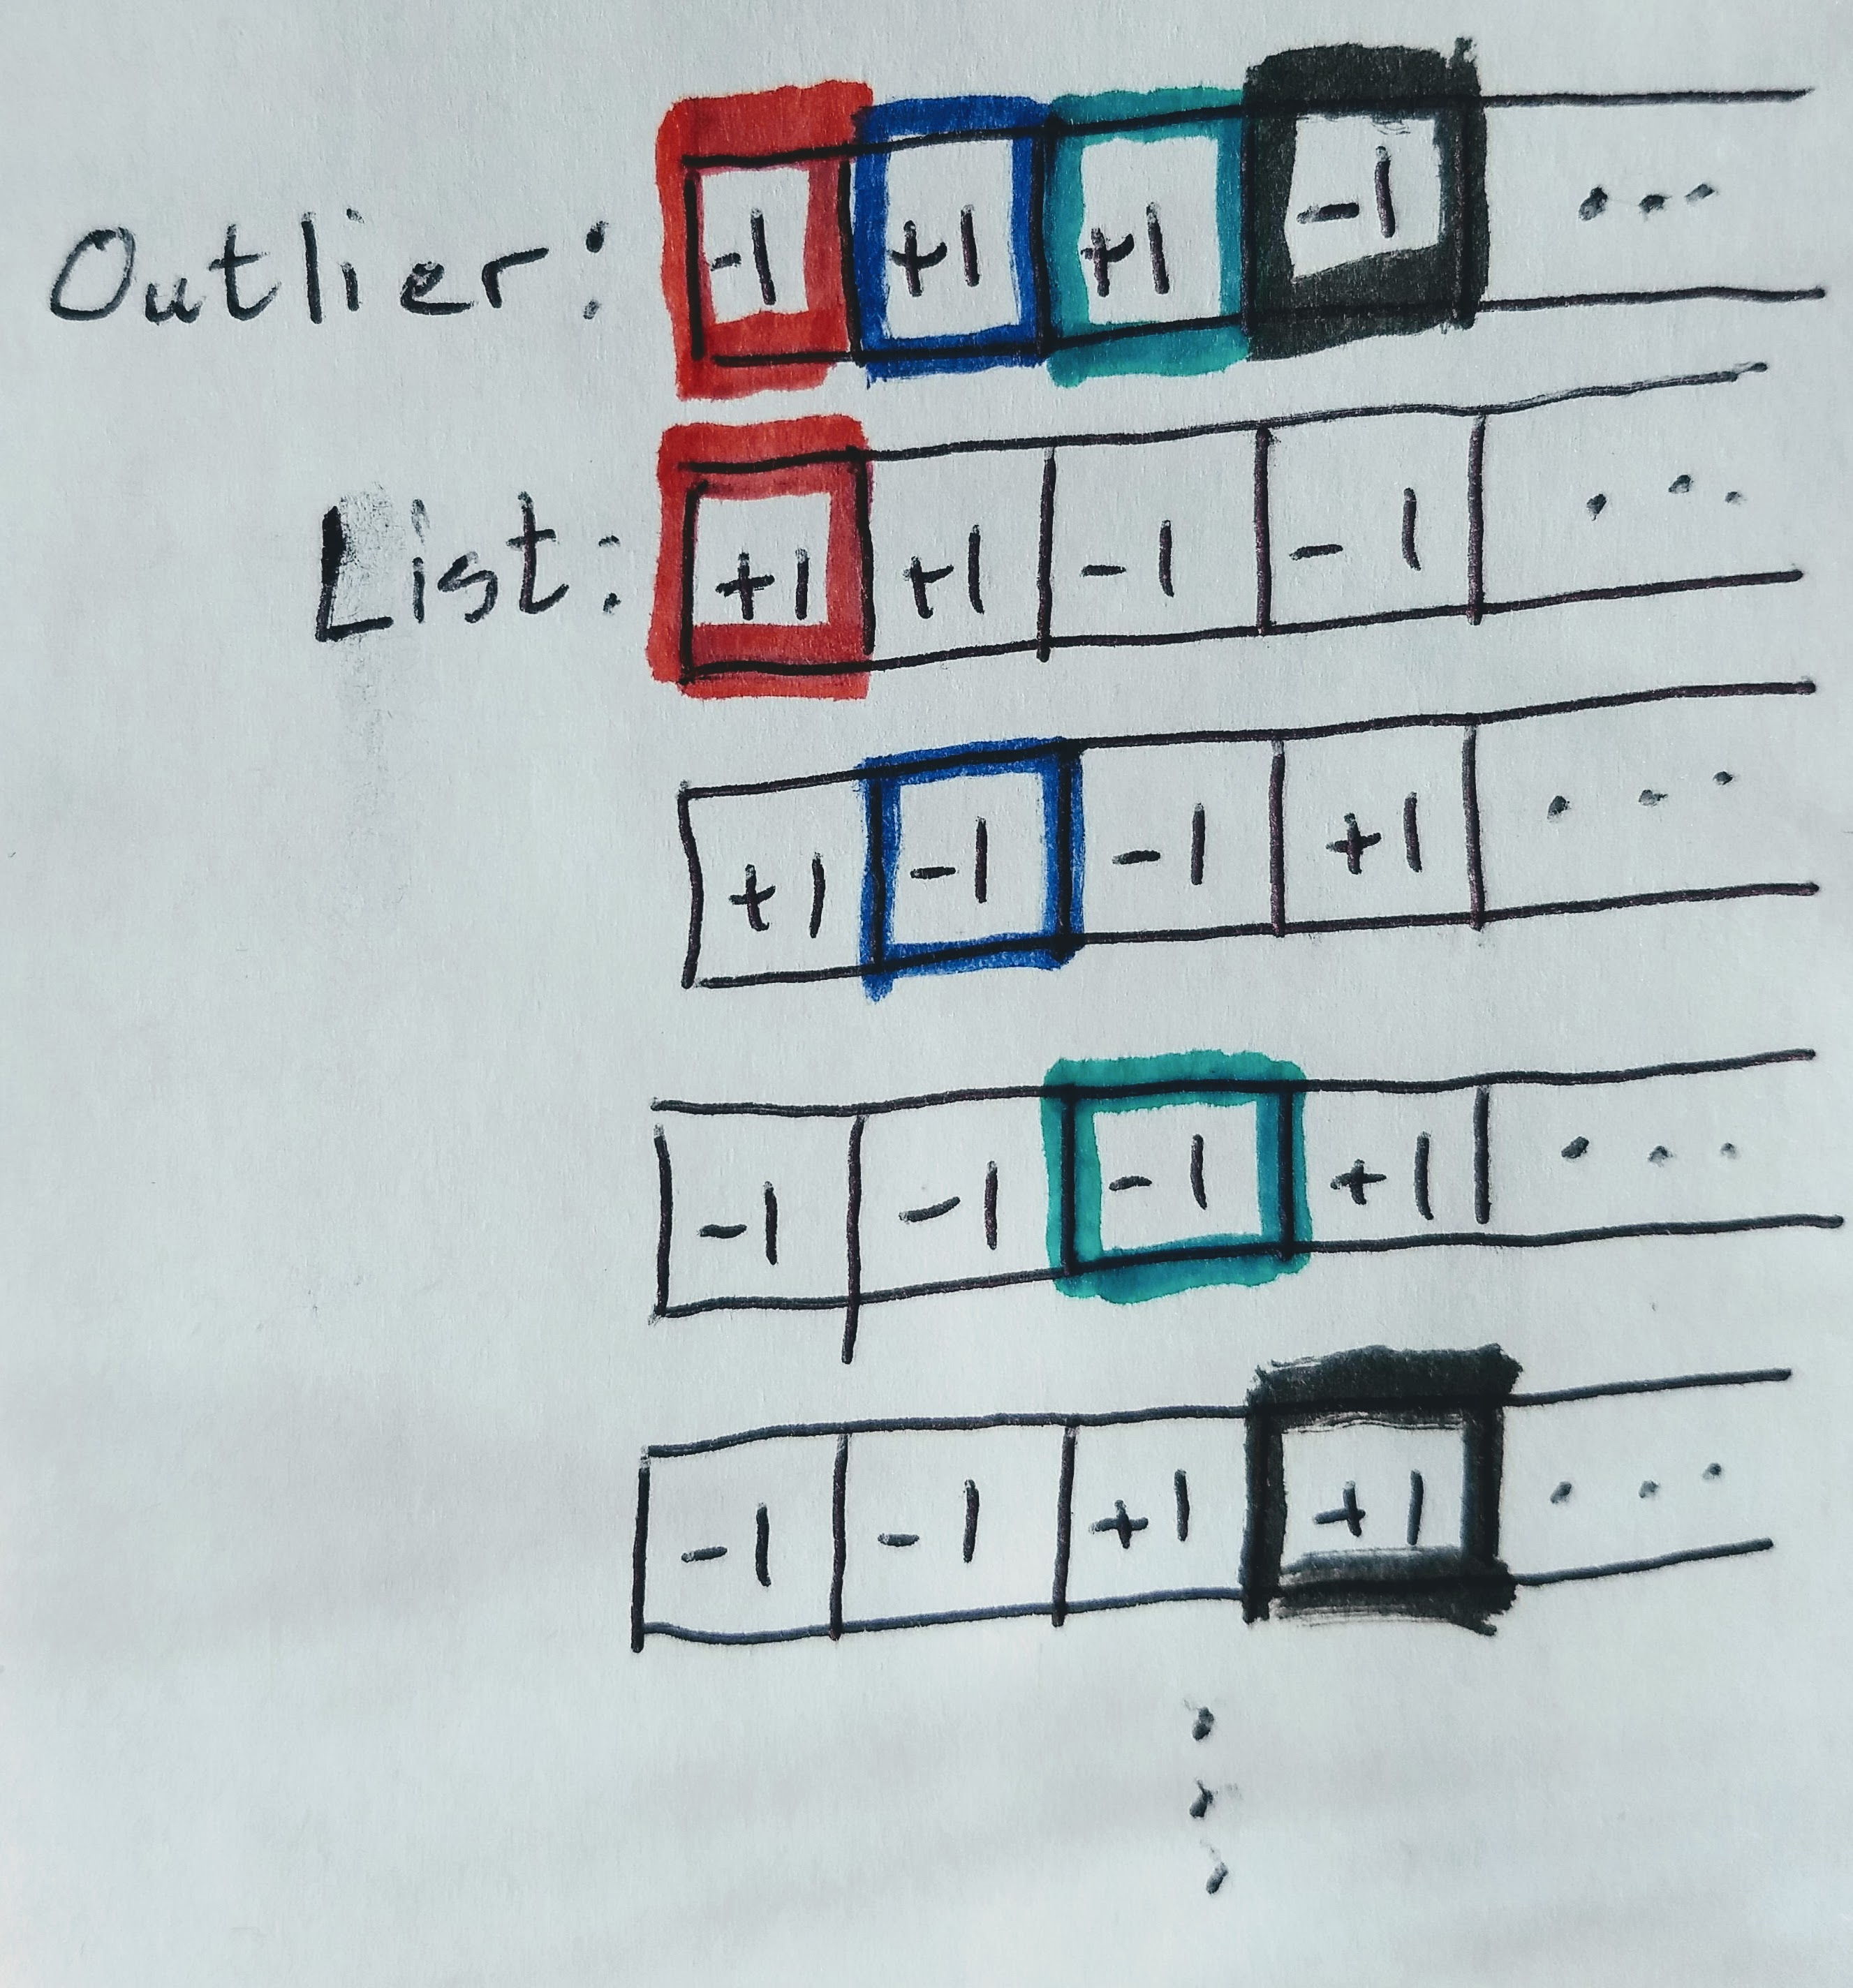
\includegraphics[width=0.5\linewidth]{figures/cantor-diag}
\end{center}
\begin{enumerate}
	\item I start by building the {\bf first} coin toss in my outlier. I look at the first toss of the first element in your list, $f(1)_1$. If I see a 0, I set my first toss to 1. If I see a 1, I set my first toss to 0. 
	\item Then I build the {\bf second} toss in my outlier. I look at the {\bf second} toss of the {\bf second} element in your list, $f(2)_2$. If I see a 0, I set my second toss to 1. If I see a 1, I set my second toss to 0.
	\item {\bf Third} toss: I look at the {\bf third} toss of the {\bf third} element in your list, $f(3)_3$. If I see a 0, I set my third toss to 1. If I see a 1, I set my third toss to 0.
	\item etc.
\end{enumerate}
By construction, the outlier cannot be in your list! We conclude the set $\Omega$ of all infinite coin tosses is not countable (i.e., \emph{uncountable}). 

\point{Remedy:} here is the first part of Kolmogorov's insight (in turn based on insights from the then-nascent theory of measure)
\begin{enumerate}
	\item Give up defining the probability by assigning it to single outcomes.
	\item Instead, assign probability to events. I.e. define $\P(A)$ for  event $A$, not $\P(\omega)$ for outcome $\omega$. 
	\item The function $\P$ is now defined on a much bigger space! Many functions defined on that large space make no sense (e.g. we could have $\P(\Omega) \neq 1$ which does not make sense). Let us use the intuition gained with example version A to extract what are the things we want to assume on $\P$. The list of what to include in order to get an interesting theory is surprisingly short:
	\begin{enumerate}
		\item Additivity of disjoint events.
		\item $\P(\Omega) = 1$.
	\end{enumerate}
\end{enumerate}

\point{Second difficulty:} we need to be careful about how we define the disjoint additivity axiom! If we allowed additivity over uncountable collections of events, we would be back the ``paradox'' at the beginning of the section, i.e. that $\P(\{\omega\}) = 0$ but \[ \P(\cup_{\omega \in \Omega} \{\omega\}) = P(\Omega) = 1. \]

\point{Remedy (continued):} assume disjoint additivity only for countable collections of events. More formally, assume that if $A_1 \in \events, A_2 \in \events, A_3 \in \events, \dots$ is a countable collection of disjoint events ($i\neq j \Longrightarrow A_i \cap A_j = \emptyset$), then 
\[ \P(\cup A_i) = \sum_{i=1}^{\infty} \P(A_i). \]

\point{Third difficulty:} a strange theorem of measure theory states that there exists no probability distribution defined on all events, $\P:2^\Omega \to [0, 1]$ such that $\P(\{\omega\}) = 0$ for all $\omega \in \Omega$.

\point{Intuition:} when $\Omega$ is uncountably infinite, $2^\Omega$ is very strange! E.g. some events cannot be described by any language (any languages that we know of proceeds by putting letters from a finite alphabet one after another; well, that can only produce a countable set of descriptions. So that mean certain paths in $\Omega$ cannot be described in  version B of the train example)! 

\point{Remedy (continued):} do not attempt to define $\P$ on all subsets of $\Omega$. Define it on a subset of events called a $\sigma$-algebra. Make the $\sigma$-algebra big enough to do all the computations we are interested in doing: taking countable unions, intersections, and complements. As we will see soon this solves our problem, in the sense that there is a $\events \subsetneq 2^\Omega$, $\P : \events \to [0, 1]$ such that $\P(\{\omega\}) = 0$ but for example $\P(A_t) = 1/2$.

 
\subsection{The axioms of probability} 

To summarize the discussion of the last section, a probability space contains three things:
\begin{enumerate}
  \item a set $\Omega$, called the sample space,
  \item a closed collection of events, $\events \subset 2^\Omega$, called a \sigmaalg,
  \item a probability measure (synonym: probability distribution), $\P : \events \to [0, 1]$.
\end{enumerate}
where:
\begin{enumerate}
  \item the \sigmaalg\ satisfies:
  \begin{enumerate}
    \item $\Omega \in \events$,
    \item $A_1 \in \events, A_2 \in \events, A_3 \in \events, \dots, \Longrightarrow \cap_{i=1}^\infty A_i \in \events$,
    \item $A \in \events \Longrightarrow A^\complement \in \events$.
  \end{enumerate} 
  \item and the probability measure satisfies:
  \begin{enumerate}
    \item $\P(\Omega) = 1$,
    \item if $A_1 \in \events, A_2 \in \events, A_3 \in \events, \dots$ is a countable collection of disjoint events ($i\neq j \Longrightarrow A_i \cap A_j = \emptyset$), then 
    \[ \P(\cup A_i) = \sum_{i=1}^{\infty} \P(A_i). \]
  \end{enumerate}
\end{enumerate}

\point{Measure:} a measure space is a very close cousin to a probability space. The axioms are identical, except for two changes:
\begin{enumerate}
	\item We remove the bound $[0, 1]$ and replace by $[0, \infty)$, and use the terminology measure (often denoted $\mu$) instead of probability, $\mu : \events \to [0, \infty)$.
	\item We modify $\P(\Omega) = 1$ into $\mu(\emptyset) = 0$. 
\end{enumerate}



\subsection{Some basic properties}\label{sec:basic-properties}

Some examples of basic properties we can derive from these axioms:
\begin{enumerate}
  \item $\P(A^\complement) = 1 - \P(A)$, \label{property:complement}
  \item if $A$ and $B$ are events that are not necessarily disjoint, $\P(A \cup B) = \P(A) + \P(B) - \P(A \cap B)$. \label{property:additivity-overlap}
\end{enumerate}

\point{Idea:} partition sets into disjoint bits, so that the disjoint additivity can be used. For part~\ref{property:complement}, use that $A$ and $A^\complement$ form a partition of $\Omega$. For part~\ref{property:additivity-overlap}, define the set subtraction as $E\backslash F = \{e \in E : e \notin F\}$, and use the partition $A\backslash B, B \backslash A, A \cap B$.

\point{Exercise:} write down the argument.

\subsection{Probability spaces as models}

\subsubsection{Coin tosses}

\point{Question:} you toss two coins, what is the probability of two heads? Note that you are not able to tell the two coins apart.

\point{Sample space:} which of these should we pick?
\begin{enumerate}
  \item $\Omega_1 = \{(H, H), (H, T), (T, H), (T, T)\}$
  \item $\Omega_2 = \{\{H, H\}, \{H, T\}, \{T, T\}\}$. 
\end{enumerate}

The best answer is $\Omega_1$, but why? Choosing between these two (essentially, selecting one of these two models) is not part of probability theory per se. Use have to use your intuition about the real world here. For example, note that if you painted one coin red and one blue, the setup of this experiment would not have changed. Hence, the model that is most useful is the one that uses lists even though we could not observe this distinction. Probability theory comes in once we have built a model, at which point inference can be carried using mathematical principles. Probability theory can help selecting model though, for example by making certain predictions for a given model, which can then be tested (for example, the long term behavior of frequencies, which is mathematically understood for a wide range of probability models).


\subsubsection{Reliability}\label{sec:reliability}

Reliable systems replicate a critical component (e.g. a power supply in a computer server) so that the whole system works as long as at least one of the two copies works. Consider an assembly line for computer servers. Suppose the first power supply assembly line is observed to put in a power supply that works $60\%$ of the time. The second  power supply assembly line  is observed to put in a power supply that works $70\%$ of the time. At delivery, both power supplies work $40\%$ of the time. 

\point{Exercise:} What is the probability that both power supplies are broken at delivery? Hint: the answer is not $12\%$. 

If you answered $12\%$, you are using a property that is \emph{not} built into (or derivable from) the axioms of probability: namely that if $\P(A \cap B) = \P(A) \P(B)$. It is an extra assumption called \emph{independence} of the events $A$ and $B$. It is kept separate because there are situation where it is useful to describe the world, and others where it is not (can you imagine a scenario where the two assembly lines are not independent?). This contrast with the disjoint union axiom of probability, which models a universal aspect of reality. 


\subsection{Statistical models}\label{sec:statistical-model}

Statistical models are built using probability models. Consider the following example:

\point{Estimation:} consider the train example, but where instead of a standard coin being used to make the decision at each step (50\%-50\% to go left or right), a \emph{biased} coin is used, i.e. where the train goes left with probability $\theta\in [0, 1]$ and right with probability $1 - \theta$. The problem is that we do not know $\theta$! Instead, we try to reconstruct $\theta$ from data (observed paths). This problem, point estimation, is one an important type of problems considered in statistics. 

\point{Frequentist models:} use not one but many probability distributions all defined on a shared space $(\Omega, \events)$:
\[ \text{frequentist model} = \{ \P_\theta : \events \to [0, 1], \theta \in \Theta\}. \]
If the index set $\Theta$ is some subset of $\R^d$, the model is called parametric, otherwise, it is called non-parametric.

\point{Bayesian models:} use only one probability distribution. Augment the space $\Omega$ to include the unknown quantity $\theta \in [0, 1]$, i.e. $\bar \Omega = [0, 1] \times \Omega$. We will go over this way of modelling in more detail when we talk about conditioning.


\subsection{Simple examples of $\sigma$-algebra}

We have seen one ``foundational'' motivation for $\sigma$-algebras. We will also see a more useful motivation soon which is that $\sigma$-algebras can encode rules of a game, but we will need to define random variables first. For now, let us look at some examples to make this concept a bit more concrete.

\begin{description}
  \item[Power set:] the power set $2^\Omega$ is always a $\sigma$-algebras on $\Omega$. For example \[\events_0 \defeq \{\{a, b, c\}, \{a, b\}, \{a, c\}, \{b, c\}, \{a\}, \{b\}, \{c\}, \emptyset\}\] is a $\sigma$-algebras on $\Omega \defeq \{a, b, c\}$.
  \item[Another discrete example:] the collection of events \[\events_1 \defeq \{\{a, b, c\}, \{a, b\}, \{c\}, \emptyset\}\] is also a \sigmaalg\ on $\Omega \defeq \{a, b, c\}$.
  \item[A non-example:] the collection $\events_2 \defeq \events_1 \cup \{\{a\}\}$ is not a \sigmaalg. Why? We have $\{a\} \in \events_2$ yet $\{a\}^\complement \notin \events_2$.
\end{description}


\subsection{More interesting examples of $\sigma$-algebra via generation}\label{sec:generated}

Let $\generators$ denote a collection of events. The machinery of this section is useful when the collection $\generators$ is ``broken,'' i.e. when it is not  a \sigmaalg\ (example: $\generators \defeq \events_2$ above). 

We would like to ``repair'' $\generators$ by adding more events until we get a closed collection of event. How can we do this is such a way that the output of the repair process is unique and well-defined? 

\begin{enumerate}
  \item \label{item:inter-sigma} Let $\events$ and $\events'$ be two \sigmaalg\ on $\Omega$. \point{Exercise:} convince yourself that their intersection $\events \cap \events'$ is also a \sigmaalg.
  \item The result in \ref{item:inter-sigma} can be generalized: if we have any collection of $\sigma$-algebras $\{\events_\alpha : \alpha \in I\}$, where $I$ is some index set (not necessarily countable), then \[ \bigcap_{\alpha \in I} \events_\alpha \] is also a \sigmaalg.
  \item Let us pick \[\{\events_\alpha : \alpha \in I\} = \{\events_\alpha : \events_\alpha \text{ is a }\sigma\text{-algebra containing }\generators\},\] then we get that the intersection of the $\events_\alpha$ is a \sigmaalg.
  \item We call this intersection the \sigmaalg\ \emph{generated} by $\generators$, denoted $\sigma(\generators)$. 
  \item Another way to think about $\sigma(\generators)$: the \emph{smallest \sigmaalg\ containing $\generators$}.
\end{enumerate}

\point{Some examples:}
\begin{enumerate}
  \item $\sigma(\events_2) = 2^{\{a,b,c\}}$.
  \item An important example where the generated \sigmaalg\ is smaller than $2^\Omega$: \emph{the Borel \sigmaalg}. To follow this example, it will help to first make the observation that infinite paths can be made in correspondence with the interval $[0, 1)$. This is done via the \emph{binary representation} of real numbers, which works schematically as follows: 
  \begin{center}
  	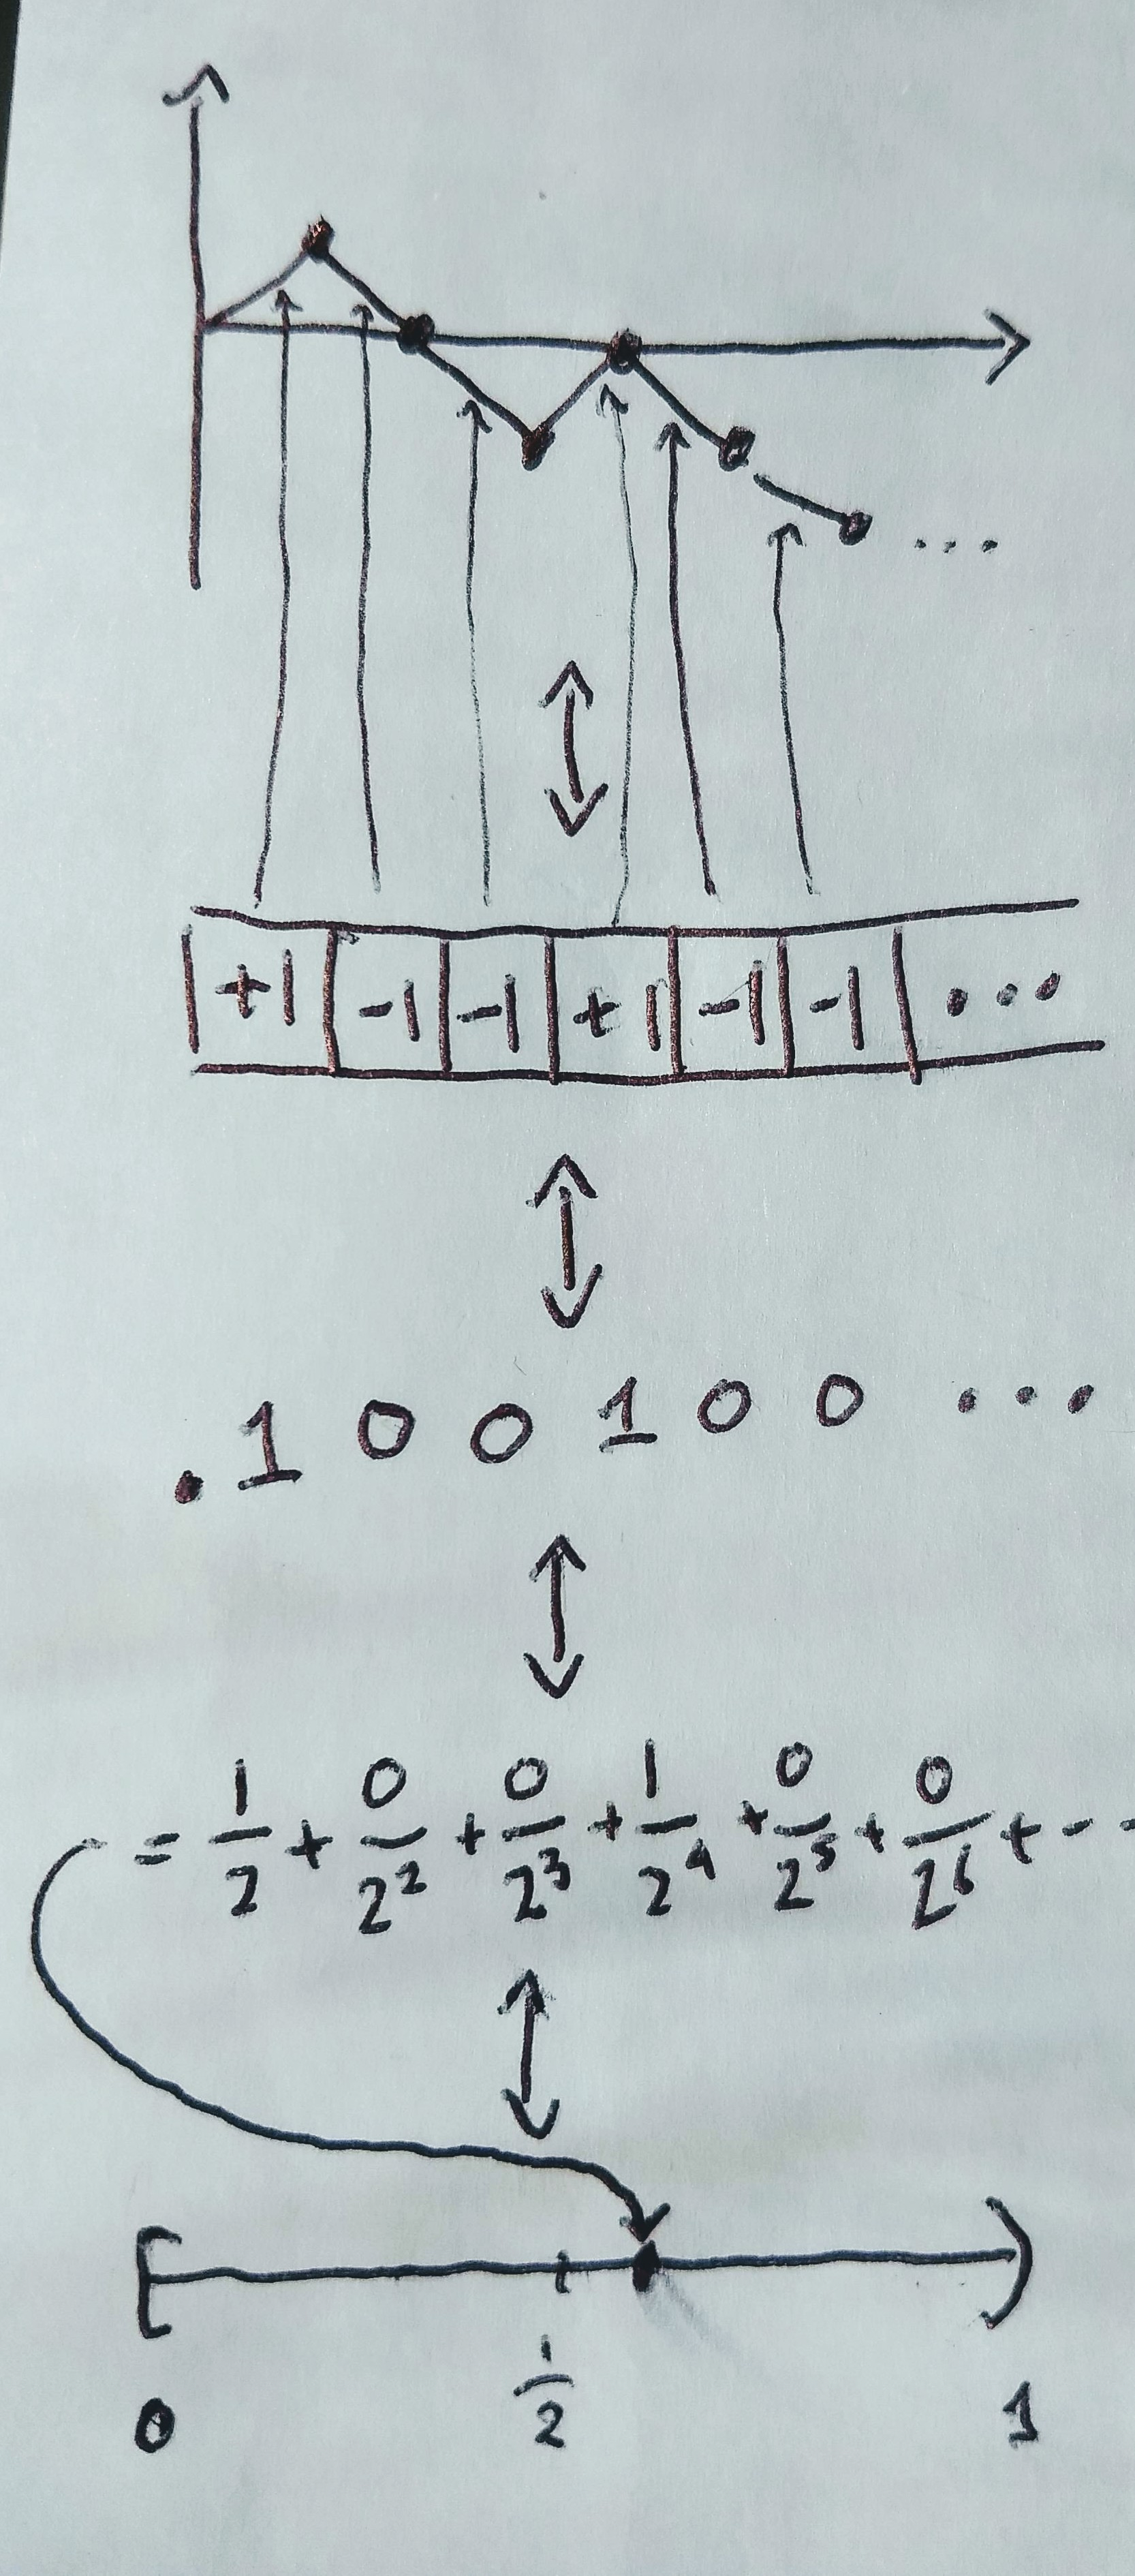
\includegraphics[width=0.3\linewidth]{figures/binary}
  \end{center} 
  This correspondence shows that many events of interest can be expressed as intervals in $[0, 1)$. For example what is the interval corresponding to ``the train goes left in the first step''? The interval $[0, 1/2)$.
  So to be able to have these intervals in our $\sigma$-algebra, we proceed as follows:
  \begin{enumerate}
    \item Take $\Omega \defeq [0, 1)$, and $\generators_\text{B} \defeq \{F : F\text{ is a finite collection of intervals}\}$.
    \item Convince yourself that $\generators$ is not a \sigmaalg.
    \item We call $\sigma(\generators_\text{B})$ the \emph{Borel \sigmaalg}, denoted $\borels$.
    \item Elements of $\borels$ are called Borel events.
    \item Some measure theory shows that $\borels$ is a proper subset of $2^{[0, 1)}$.
  \end{enumerate}
\end{enumerate}


\subsection{Simple examples of probability measures}

\begin{description}
  \item[Discrete probability measure:] assume you are given a countable sample space $\Omega$ and a function $p: \Omega \to [0, 1]$ called a \PMF. Define, for any event $A \in \events$: \[ \P(A) \defeq \sum_{\omega \in A} p(\omega). \] Check that this definition satisfies the axioms of probability. Note: do not confuse $p$ and $\P$, as they take different types of inputs!
  \item[Conditional probabilities:] fix an event $E$ which you can interpret as some data, with $\P(E) > 0$. Define a new probability distribution as \[ \P'(A) = \frac{P(A \cap E)}{\P(E)}. \] Check $\P'$ is indeed a probability. If $\P$ is some agent's belief before observing $E$, $\P'$ can be interpreted as the optimal way for the agent to update its belief after observing $E$. This updated belief is notated $\P'(\cdot) = \P(\cdot | E)$ and is called the conditional probability given $E$. From now on, if we write $\P(A | E)$ we will assume $\P(E) > 0$ implicitly.
  \item[The uniform probability measure:] some (surprisingly heavy) measure theory shows that there exists a probability measure on $\borels$ such that $\P([a, b)) = b - a$ for all $0 \le a \le b < 1$.
\end{description}

This second example is actually enough to build a rich theory! How? Using random variables and their distributions, which we will cover shortly.


\point{Example of a measure:} the Lebesgue measure is the same as the uniform probability distribution, except that it is defined on $\R$ instead of $[0, 1)$. 


\subsection{Computations for discrete models}\label{sec:computation-discrete}

We already have enough tools to formulate and solve many interesting problems involving \emph{discrete} models (i.e. with $|\Omega| < \infty$). 

\point{Exercises:} You can solve the following problems by explicitly enumerating all the possible scenarios. However, I ask here that you go beyond and that you formalize your reasoning, by (1) setting up a probability model using set theory only, no English allowed,\footnote{Obviously, in general I do recommend a mix of English and math for clarity, but probability beginners tend to rely too much on the former.} and (2), use the axioms of probability to solve the problem. All you need is the following two tools.

\point{Tool 1: chain rule.} For any event $A$, $B$, 
\[\P(A \cap B) = \P(A) \P(B | A) \;\; (= \P(B) \P(A | B)).\] 

\point{Tool 2: law of total probability (version 1). } Suppose $B_1, B_2, \dots$ is a partition of $\Omega$, then
\[ \P(E) = \sum_i \P(E \cap B_i) \;\; \left(= \sum_i \P(B_i) \P(E | B_i)\right). \]

\point{Proposed strategy:} build the model and list the known (conditional) probabilities. Write the (conditional) probability you wish to compute. Then reintroduce the ``missing'' variable in this last probability using the law of total probability and the chain rule.  

\begin{enumerate}
	\item Prove that the two ``tools'' follow from the axioms of probability.
	\item An HIV test has the following two modes of failure:
	\begin{itemize}
		\item When a patient has the disease, the test will still be negative 2\% of the time (false negative)
		\item When a patient does not have the disease, the test will turn positive 1\% of the time (false positive)
	\end{itemize}
	Given that the test is positive, what is the updated (posterior) probability that the patient is indeed affected by HIV?
	% ~33

	Suppose now 25\% of the population has HIV.
	Given that the test is positive, what is the updated (posterior) probability that the patient is indeed affected by HIV? What happens if the prevalence of the disease is very small instead?
	% ~97%
	\item There are 3 kindergarten classrooms and 9 kindergarten students in a school. The children are lined up and assigned to classrooms in turn. The principal claims the assignment is uniform over all possible assignments. The classrooms 
	have the following capacities:

	\begin{itemize}
		\item Classroom (a): 4 students

		\item Classroom (b): 3 students
		\item Classroom (c): 2 students
	\end{itemize}

	You are fifth in the list of children. What is the probability that you get assigned to class (a)? 
\end{enumerate}


\subsection{Exercise set 1}

\begin{enumerate}
	\item Solve the exercise in Section~\ref{sec:basic-properties}
	\item Solve the exercise in Section~\ref{sec:reliability}
	\item Solve the exercise in Section~\ref{sec:computation-discrete}
\end{enumerate}


\subsection{Solutions for exercise set 1}

\subsubsection{Basic properties}

First, not that additivity for a countable collection implies additivity for a pair, by taking $A_3 = A_4 = A_5 = \emptyset$. Since $A$ and $A^\complement$ are disjoint, $P(A) + P(A^\complement) = 1$, and hence the first simple property. 

For the second property we make use of the following:
\begin{enumerate}
	\item $\{A\backslash B, A \cap B\}$ is a partition of $A$; hence $\P(A\backslash B) + \P(A \cap B) = \P(A)$;
	\item $\{B\backslash A, A \cap B\}$ is a partition of $B$; hence $\P(B\backslash A) + \P(A \cap B) = \P(B)$;
	\item $\{A\backslash B, B \backslash A, A \cap B\}$ is a partition of $A \cup B$;  hence $\P(A\backslash B) + \P(B\backslash A)+ \P(A \cap B) = \P(A \cup B)$.
\end{enumerate}
Now substitute $\P(A\backslash B)$ in the equation in 3 above using equation in 1 above as well as $\P(B\backslash A)$ using equation in 2.


\subsubsection{Reliability problem}

Define $\Omega = \{(0,0), (0,1), (1,0), (1,1)\}$ where element $\omega = (i, j)$ encodes if the first power supply works ($i = 1$, otherwise $i=0$) and if the second power supply works ($j = 1$, otherwise $j=0$). Define $W_k$ as the event that power supply $k\in \{1, 2\}$ works, i.e. $W_1 = \{(1,0), (1,1)\}$ and $W_2 = \{(0,1), (1,1)\}$. We know:
\begin{enumerate}
	\item $\P(W_1 \cap W_2) = 4/10$, (by the way sometimes denoted just $\P(W_1 W_2)$), 
	\item $\P(W_1) = 6/10$,
	\item $\P(W_2) = 7/10$.
\end{enumerate}
The goal is to compute $\P(W_1^\complement W_2^\complement)$. 

First, get rid of the complement. How to do so? Use a result from set theory:

\point{De Morgan's ``Laws'':} distributing complements swap unions to intersections and vice versa, i.e. $(A \cup B)^\complement = A^\complement \cap B^\complement$;  $(A \cap B)^\complement = A^\complement \cup B^\complement$. E.g., using an example from wikipedia, the search query ``NOT (cars OR trucks)'' is the same as ``(NOT cars) AND (NOT trucks)''.

Then we have using De Morgan and the first property from previous question:
\[ \P(W_1^\complement \cap W_2^\complement) = \P((W_1 \cup W_2)^\complement) = 1 - \P(W_1 \cup W_2). \]

Finally, using the second property:
\[ \P(W_1 \cup W_2) = \P(W_1) + \P(W_2) - \P(W_1 \cap W_2) = 6/10 + 7/10 - 4/10 = 9/10. \]

Hence the answer is $1 - 9/10 = 1/10.$


\subsubsection{Discrete computation}

\point{Tools:} Chain rule follows directly from the definitions:
\[ \P(A) \P(B | A) = \P(A) \frac{\P(A \cap B)}{\P(A)} = \P(A \cap B). \]

To establish the law of total probability (version 1), first show that $\{E \cap B_1, E \cap B_2, \dots, \dots\}$ is a partition of $E$. The result then follows from countable additivity.

\point{Bayes rule:} For the HIV test, define the following events: $H$, the event that HIV is present, and $E$ the observation (a test turned positive). We know $\P(H) = 25\% = 0.25$, $\P(E | H^\complement) = 1\%$ and $\P(E^\complement | H) = 2\%$. To help visualize this, you may want to draw a decision tree where the first branching is done according to $H$ and $H^\complement$, and the second branching, by further refining via intersections with  $E$ and $E^\complement$. We seek to compute $\P(H|E)$.

Notice that $H$ and $H^\complement$ form a partition of $\Omega$. Using this fact and the law of total probability, we obtain what is called Bayes rule:
\begin{align*}
	\P(H|E) &= \frac{\P(H \cap E)}{\P(E)} \\
	&= \frac{\P(H) \P(E | H)}{\P(H) \P(E | H) + \P(H^\complement) \P(E | H^\complement)} \\
	&= \frac{0.25 \cdot (1-0.02)}{0.25 \cdot (1-0.02) + 0.75 \cdot 0.01} \approx 97\%
\end{align*}

Now what happens if the prevalence $\rho$ of the disease is very small? Generalizing the equation above, we get:
\[ \P_\rho(H|E) = \frac{1}{1 + \frac{1-\rho}{\rho}\frac{0.01}{1 - 0.02}}, \]
hence as $\rho \downarrow 0$, we get $\P_\rho(H|E) \to 0$, which is kind of surprising.

\point{Combinatorics problem:} 
\[ \Omega = \{(C_1, C_2, C_3):\{C_1, C_2, C_3\} \text{ partitions }\{1, 2, \dots, 9\}, |C_1| = 4, |C_2| = 3, |C_3| = 2\}. \]
The definition of uniform assignment is then, for any $S \subset \Omega$:
\[ \P(S) = \frac{|S|}{|\Omega|}. \]
Here we are interested in an even $T$ which can be described as:
\[ T = \{(C_1, C_2, C_3):\{C_1, C_2, C_3\} \text{ partitions }\{1, 2, \dots, 8\}, |C_1| = 3, |C_2| = 3, |C_3| = 2\}.  \]
A first solution is to compute $|\Omega|$ and $|T|$. 
To do so use a decision tree with in the first level, events capturing the assignment of the first classroom:
\[ E^1_C = \{\omega \in \Omega : \omega_1 = C\}, \]
then, at the next two levels, events capturing the assignment of the second and third classroom:
\[ E^i_C = \{\omega \in \Omega : \omega_i = C\}. \]
Using the fact that the number of subsets of size $k$ from an inventory of size $n$ is $\binom{n}{k}$, you will find that $\Omega$ can be decomposed as a regular tree with branching factors $\binom{9}{4}$, $\binom{5}{3}$, $1$, and thus:
\[ |\Omega| = \frac{9!}{4! 3! 2!}. \]
Similarly for $T$, 
\[ |T| = \frac{8!}{3! 3! 2!}, \]
thus $\P(T) = 4/9$.

A second solution:
\[ \Omega = \{(a_1, a_2, \dots, a_9) : \cup \{a_i\} = \{1, 2, \dots, 9\}\}, \]
where $a_i$ is the assignment of student $i$, identifying $\{1, 2, 3, 4\}$ as the seats for the first classroom, $\{5, 6, 7\}$, for the second. Then use the events $E_i = \{\omega : \omega_5 = i\}$. We have $|E_i| = |E_j|$ and the event of interest is $E_1 \cup E_2 \cup E_3 \cup E_4$. Thus:
\[ \P(E_1 \cup E_2 \cup E_3 \cup E_4) = \frac{4 |E_1|}{9 |E_1|} = 4/9. \]


\subsection{Random variables}

\point{Informal definition:}
\begin{itemize}
  \item A random variable is often used to encode a measurement, for example, in the previous train example, whether the train goes left or right at time step 3.
  \item Random variables are used to model partial observability of the world. In contrast to each outcome $\omega \in \Omega$, which contains all the information possible within the model, a random variable can be defined to ``forget'' information. For example, you may only known the position of the train at time steps 1 and 6, and what happens in between is unknown.
  \item Another use of random variables is to express a quantity that is unknown, but that we would like to have the probability of. A concept that I call a ``query.''
\end{itemize}

\point{Pre-requisite for the formal definition:} if $f : S \to T$ is some function, we can lift function evaluation, which takes as input points and returns points $f(x) \in T$ for $x \in S$, into function evaluation taking as input a set and returning a set, i.e. for $A \subset S$, $f(A) = \{f(x) : x \in A\}$. 
\begin{center}
	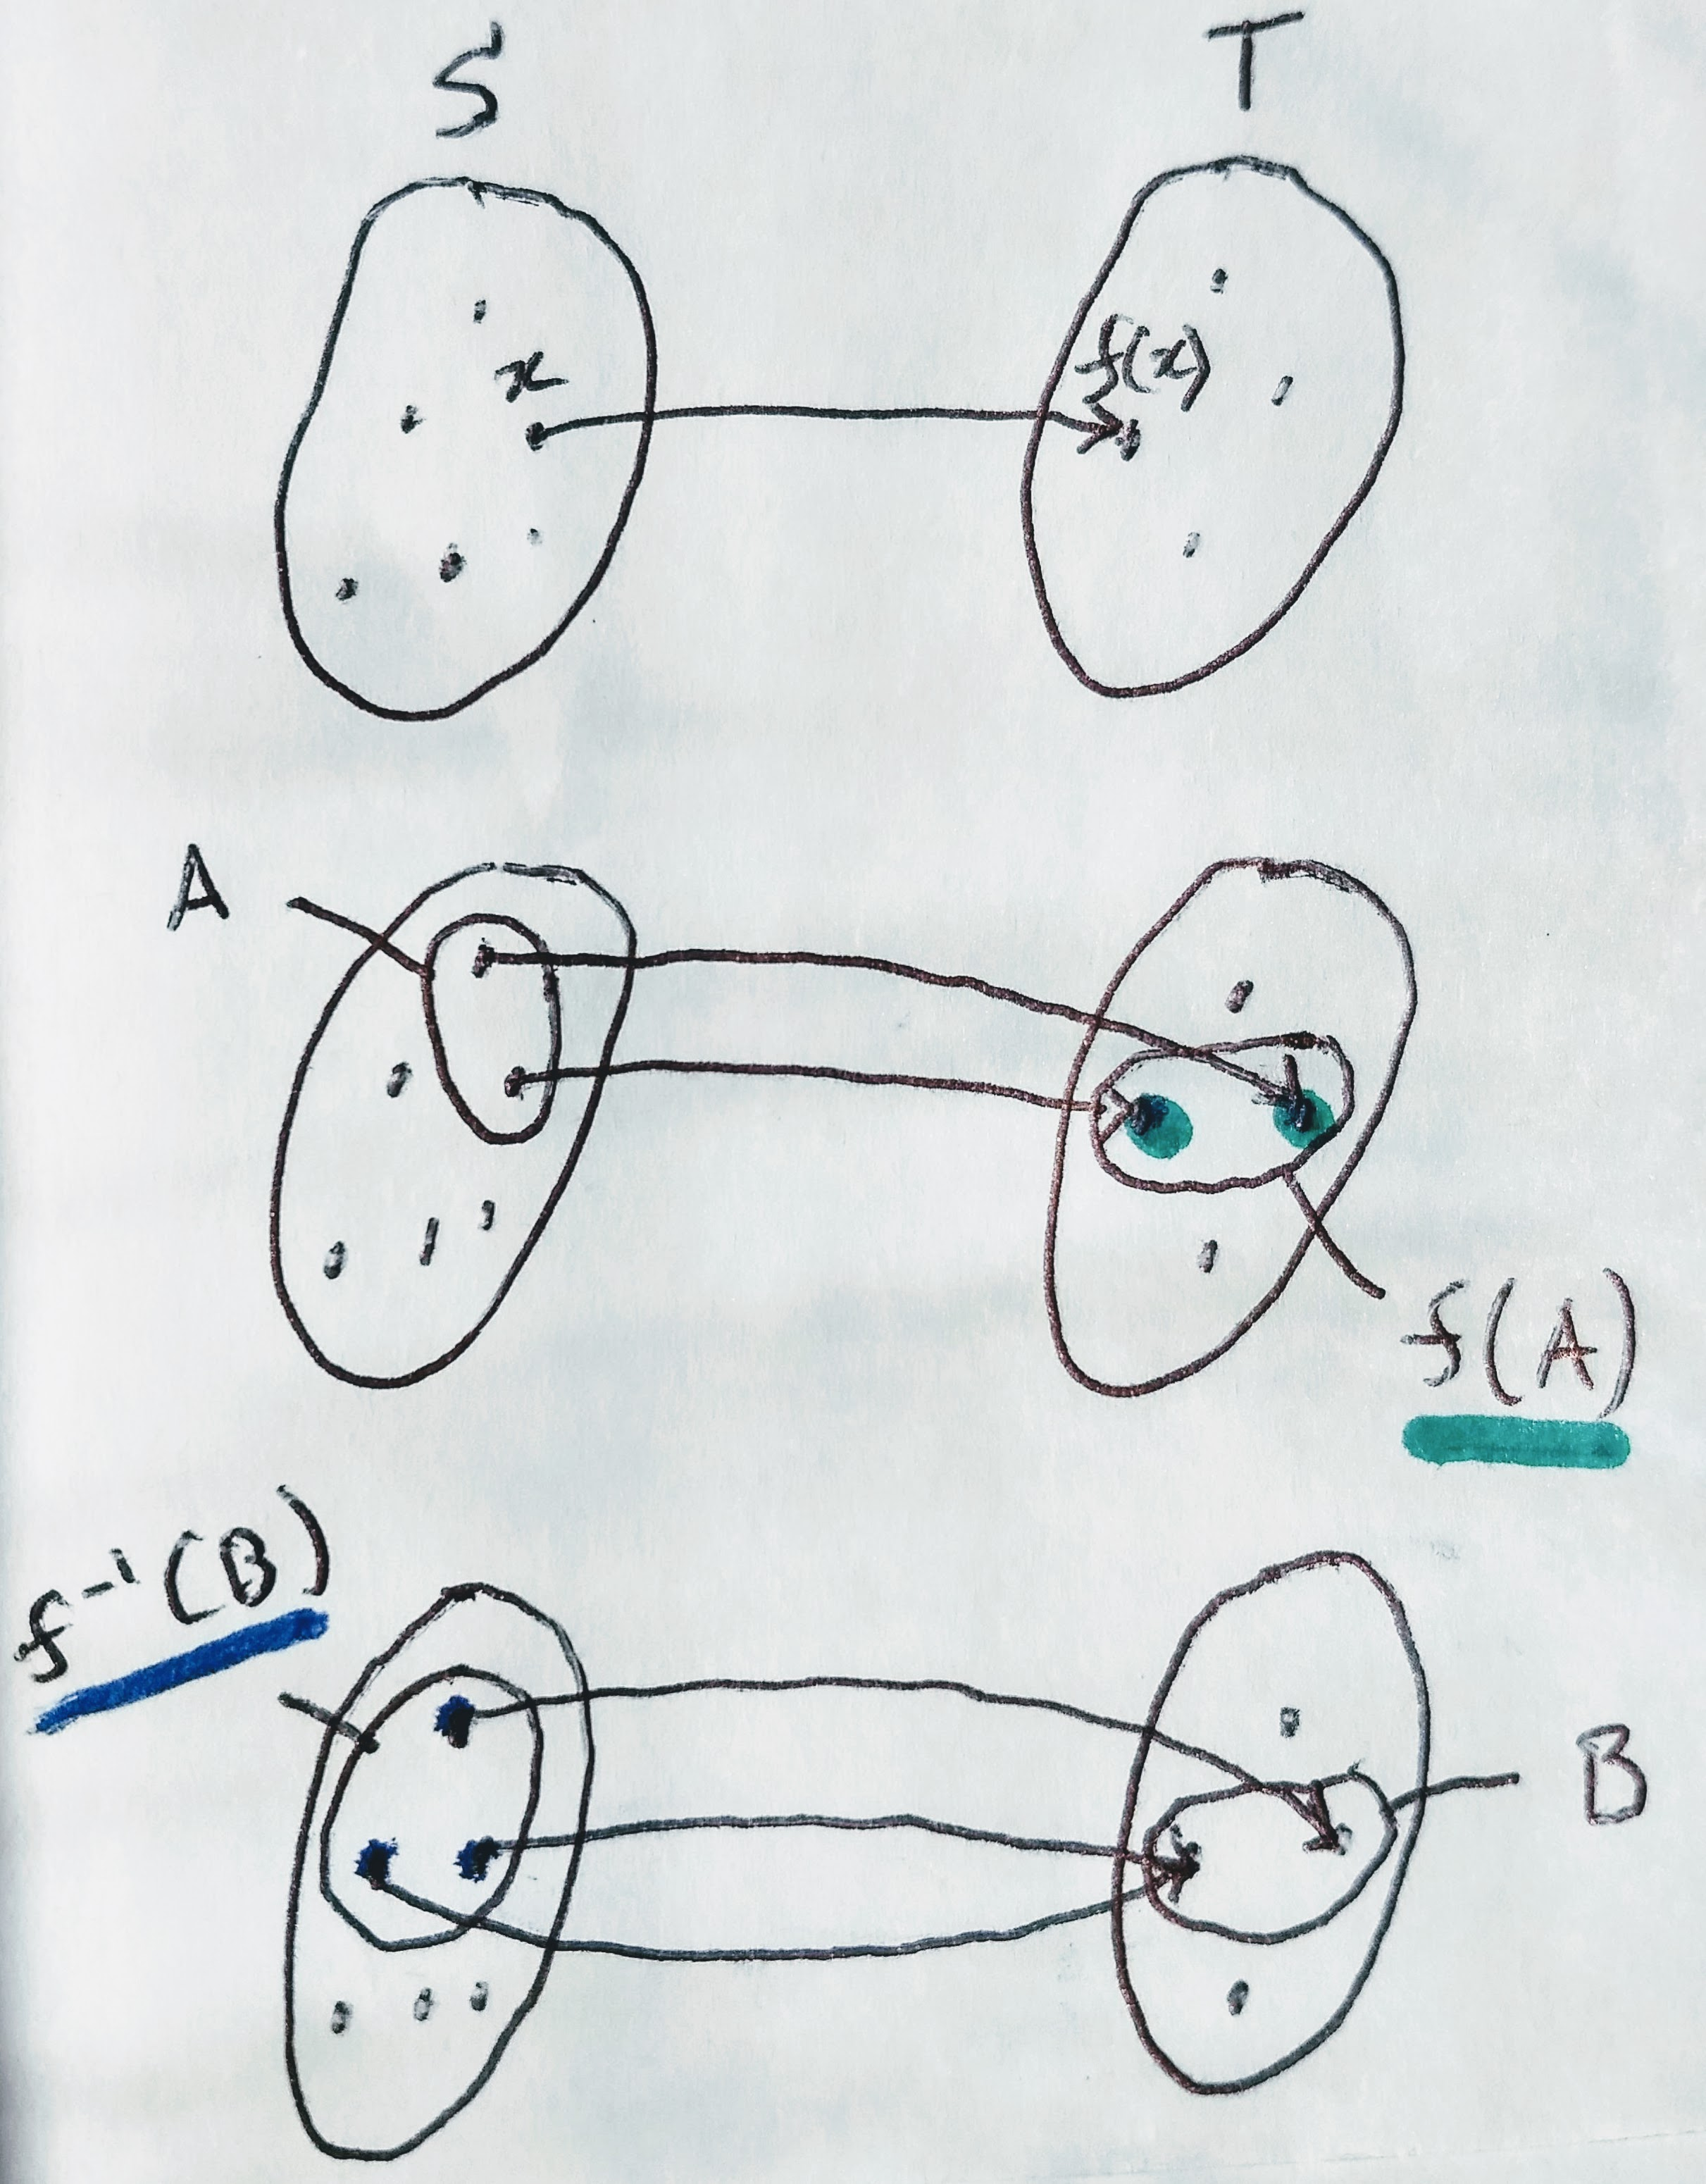
\includegraphics[width=0.3\linewidth]{figures/maps}
\end{center}
Note that we abuse the notation and use the same symbol for lifted function evaluation, but no confusion can arise because of the type of the input. We do the same for lifted function inverse: for $B \subset T$, $f^{-1}(B) = \{x \in S : f(x) \in B\}$. The lifted inverse is nice because it always exists: the set it returns can be empty or have cardinality larger than one, but it is still a set.

\point{We can now formally define random variables:}
\begin{enumerate}
  \item Let $(\Omega, \events, \P)$ denote a probability space,
  \item then a (real) random variable $X$ is:
  \begin{enumerate}
    \item a map, $X : \Omega \to \R$,\footnote{Technically, we add two points to the real line, $+\infty$ and $-\infty$, to ensure for example that limits of say increasing random variables are guaranteed to be random variables even if the sequence diverges for some outcomes $\omega$.} 
    \item \label{rv:condition} such that $X^{-1}(A) \in \events$ for all $A \in \borels$.
  \end{enumerate}
\end{enumerate}
\begin{center}
	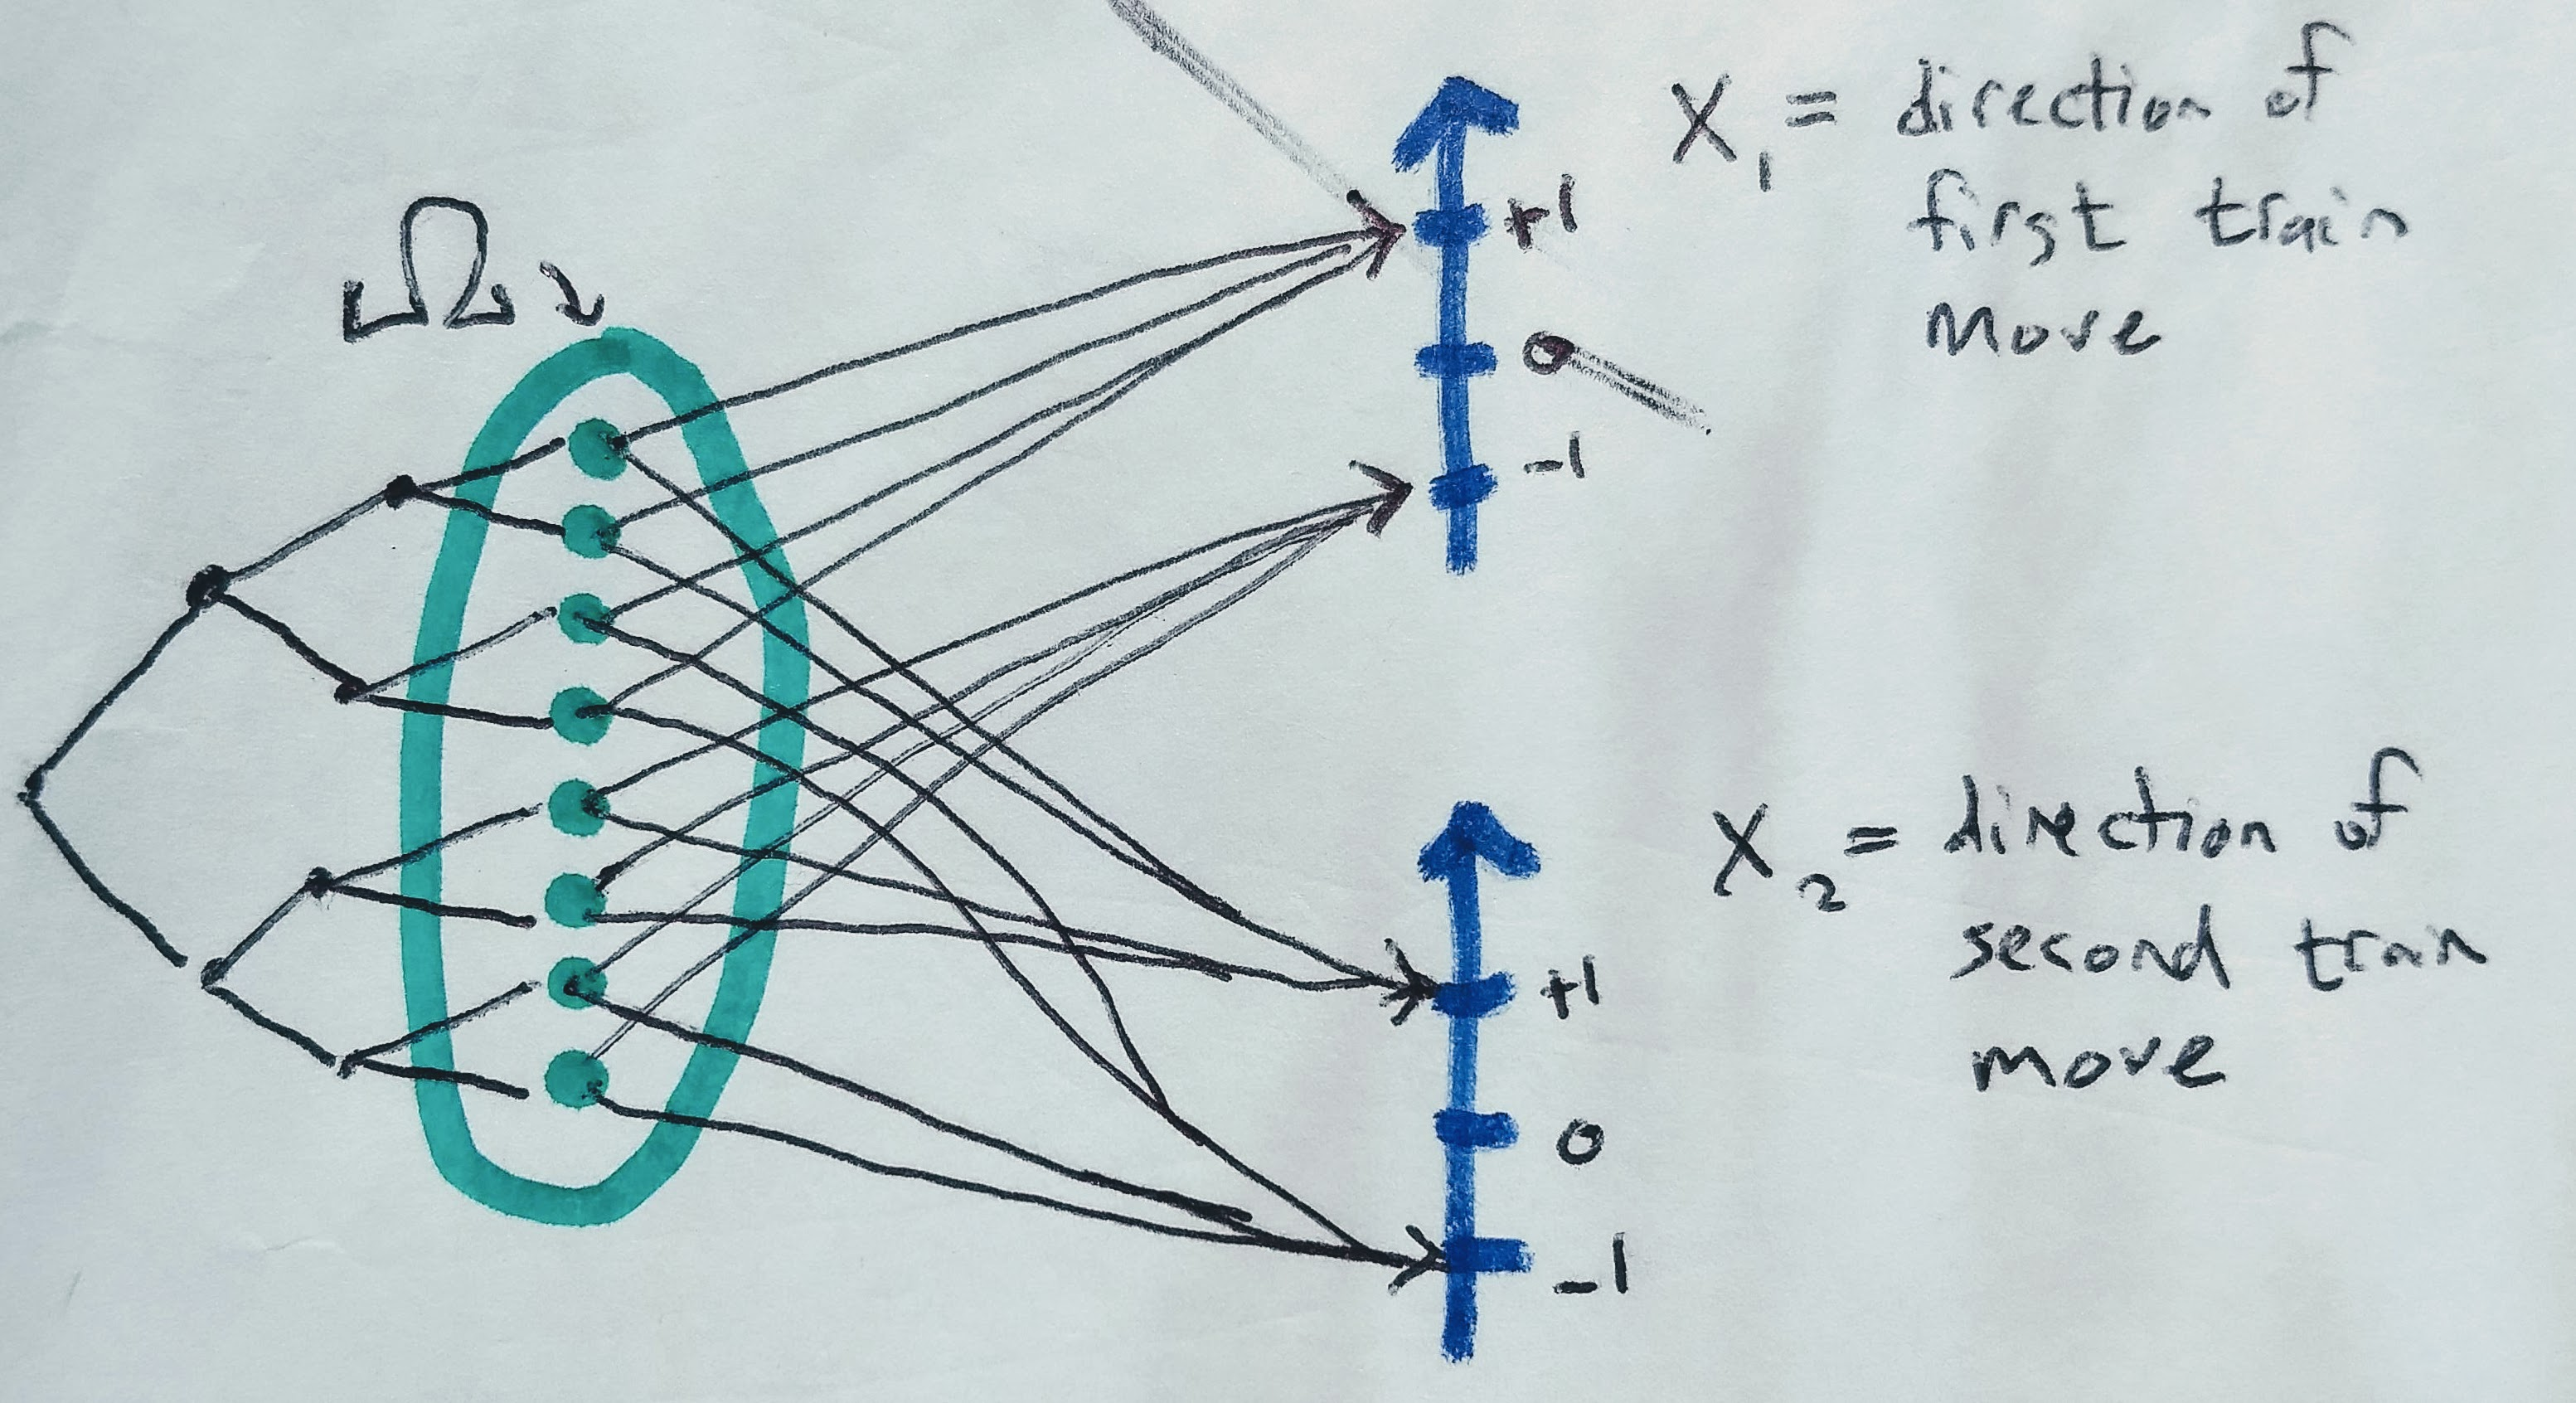
\includegraphics[width=0.6\linewidth]{figures/rvs}
\end{center}

\point{Why} do we need condition \ref{rv:condition}? Often, we will ask questions like ``what states of the worlds can yield an observation in $A$?'' In set theory, the set of such states (outcomes) is $X^{-1}(A)$. Now, we want to be able to compute the probability of this set of outcomes, so we require that $X^{-1}(A)$ be an event (i.e. in the \sigmaalg).
\begin{center}
	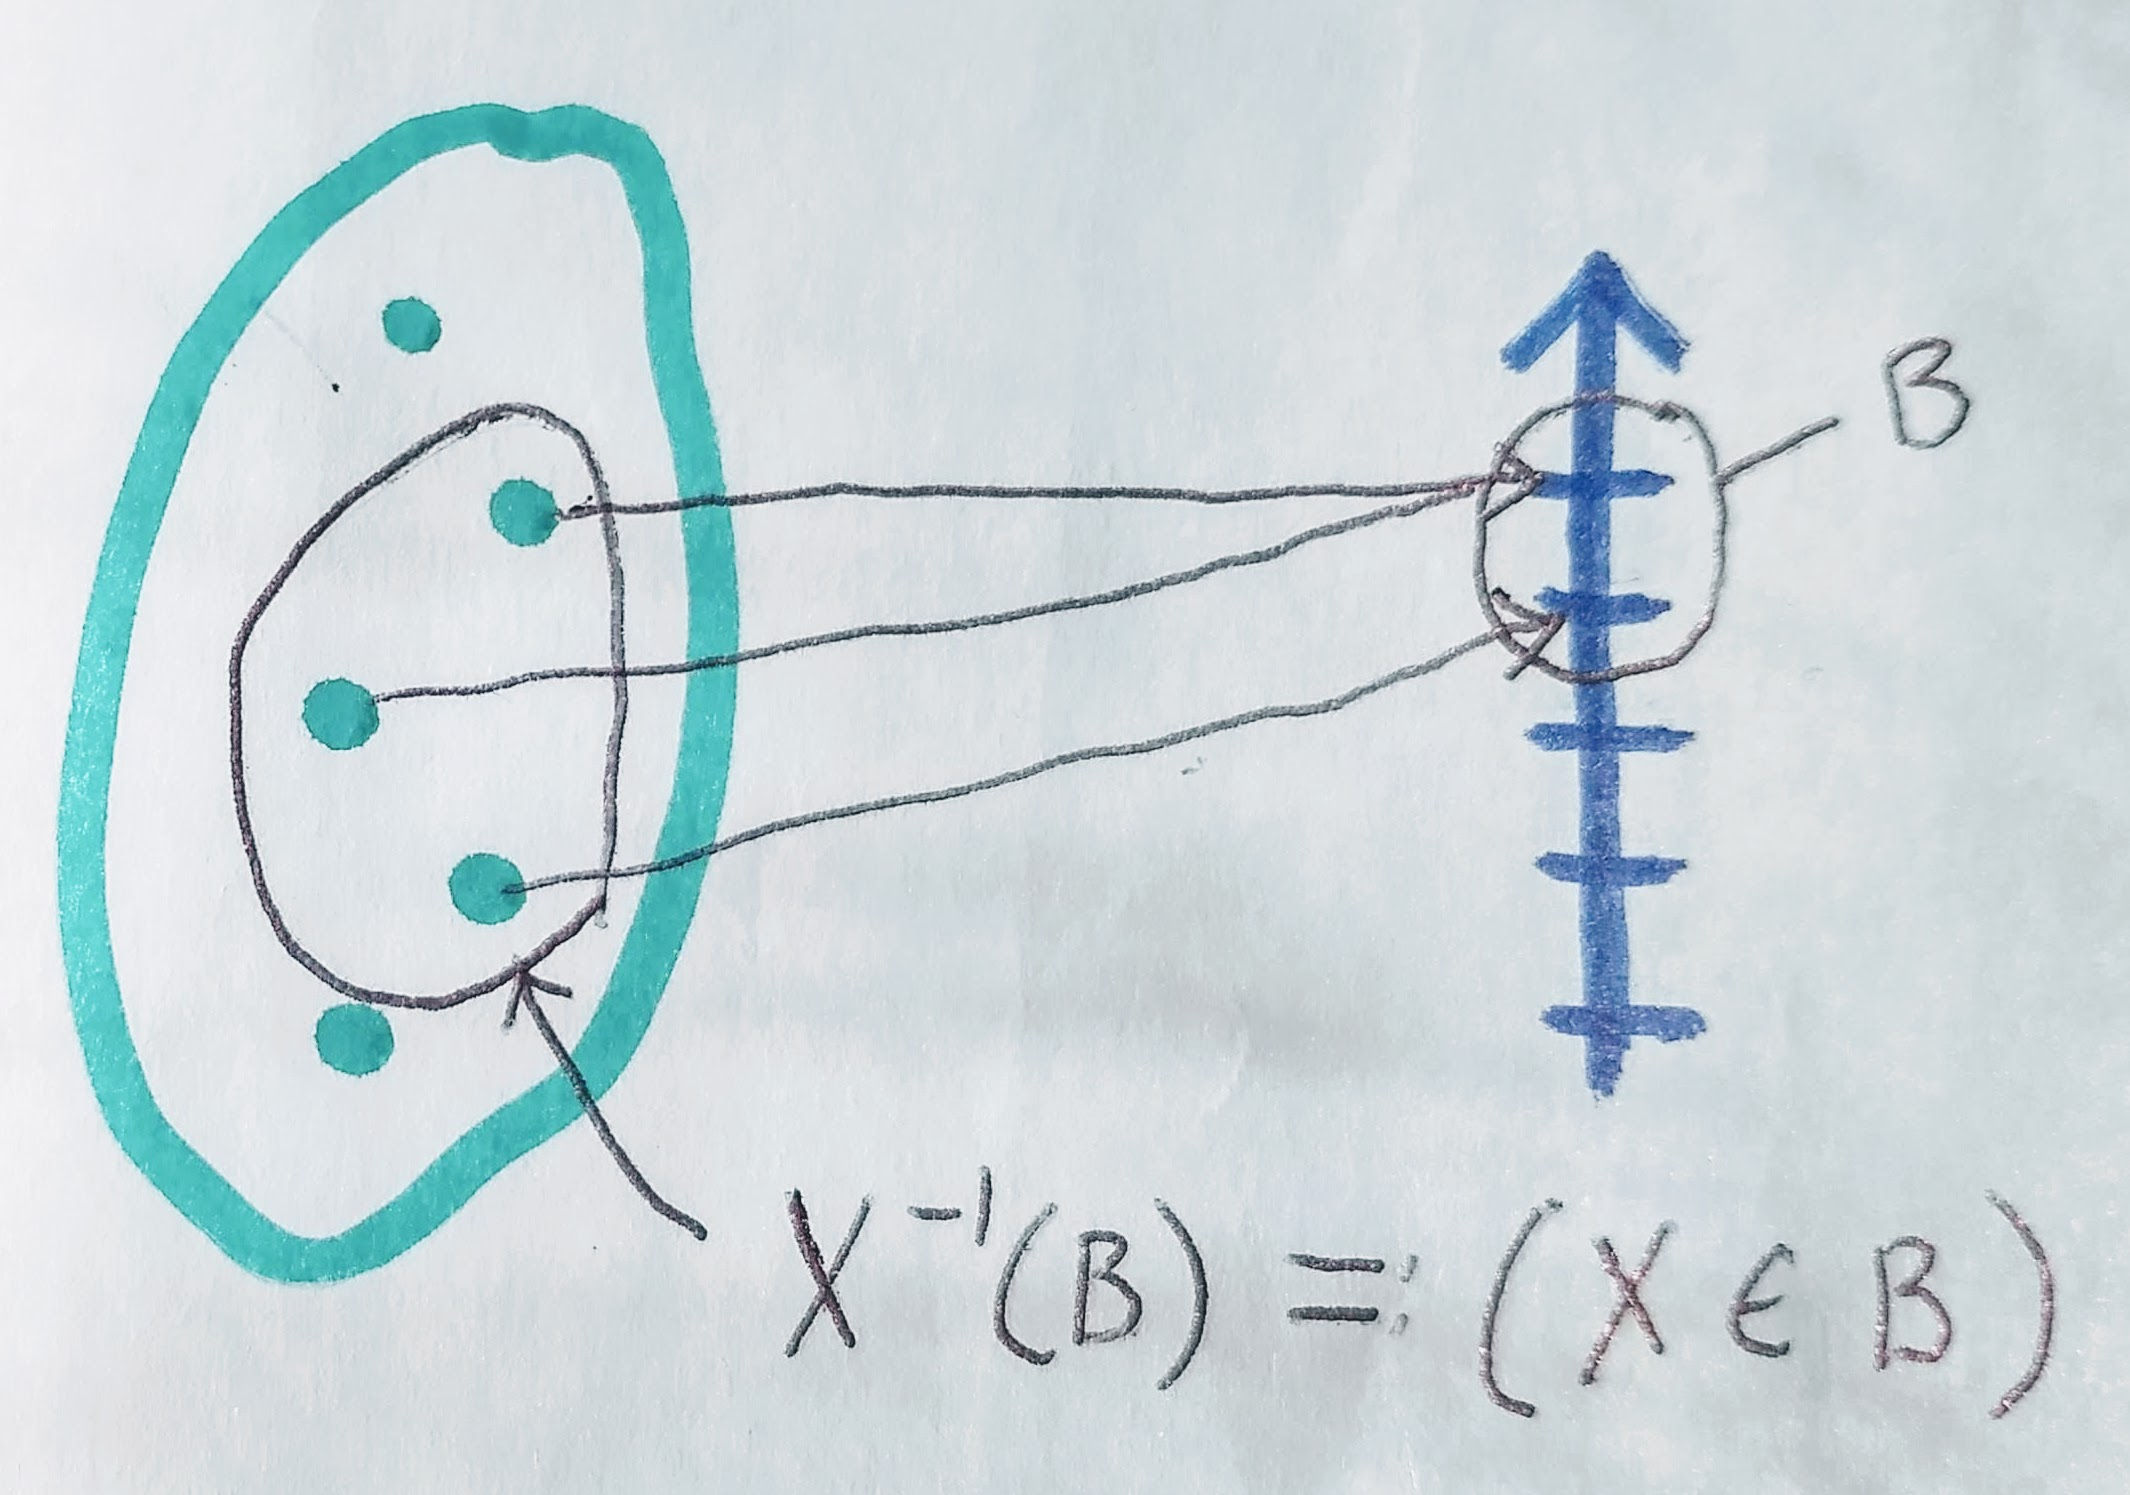
\includegraphics[width=0.5\linewidth]{figures/inverse}
\end{center}

\point{Note:} random variables are especially interesting when we define more than one on the same sample space. 

\point{Synonym:} ``$X$ is a measurable function.'' 

\point{Notes:}
\begin{itemize}
  \item Observations are not always real numbers, for example, they could be colours, the nodes in a discrete graph, or even a graph. Let $\states$ denotes the set of say all colours that could be potentially observed, $\states = \{$blue, red, yellow$\}$. We can modify our definition above to get colour-valued random variables (terminology: ``random colours''). This is done as follows:
  \begin{itemize}
    \item In the definition of real random variable, replace ``$\R$'' by ``$\states$.''
    \item Since we need a collection of sets on $\states$ in \ref{rv:condition}, let us assume we have a (second) \sigmaalg\ $\events_\states$ on $\states$ as well as on $\Omega$.
    \item Therefore, we see that all we really need is a \sigmaalg\ on the input space $\Omega$, and one on the output space \sigmaalg. Notation: a random colour is a $(\events \to \events_\states)$-measurable function.
  \end{itemize}
  \item Using this idea, we will later define random vectors (vector-valued random variable), random graphs, random sets, random functions, and even random probability measures!
  \item (Real) random variables and random vectors are special though, as they will later allow us to define the notion of expectation (not possible with colours, as we cannot for example ``add colours''). More on this later!
\end{itemize}

\point{Terminology:} values in the set $\states$ are called \emph{realizations}, and are often denoted with the small-cap version of the random variable, e.g. a realization of $X$ is denoted $x = X(\omega)$. This distinction is useful for example to distinguish $f(x)$, which is just function evaluation, from $f(X)$, which is the construction of a new random variable obtained by composing $f$ and $X$ (composition is reviewed in the next section).

\point{Warning:} make sure you follow the type conventions! For example, $\P($red$)$ or $\P(X)$ are not defined!\footnote{Some authors do give a meaning to the latter, but it is not what you think! We will see this meaning, namely the expectation of $X$, later.}


\subsection{Compositions of random variables}\label{sec:composition-of-rv}

\point{Recall:} $g \circ h$ means a new function that first applies $h$ to the input, then plugs in the intermediate quantity into $g$: $g \circ h(x) = g(h(x))$. 

\point{Convention:} use capital letters only for the random variables mapping elements from the sample space $\Omega \to \states$. Use standard function notation ($g, h$, etc) for subsequent transformations $g : \states \to \states'$  of the output of $X$. E.g. $g \circ X = g(X)$. 

\point{Exercise:} show that the composition $g(X)$ of a random variable $X$ with a measurable function $g$ is a random variable.

\point{Convention:} from now on, we will implicitly assume all functions involved are measurable. 


\subsection{The graph of a random variable}

In the special case where $\Omega = \R$, we can plot the \emph{graph} real random variables $X : \Omega \to \R$. While in practice $\Omega$ is usually much more complicated, looking at simple examples where $\Omega = \R$ is a powerful technique to get some intuition on several results we will cover in the next few weeks. Note that measurability is much weaker than continuity, so the the graph of random variables can be quite pathological in general. 
\begin{center}
	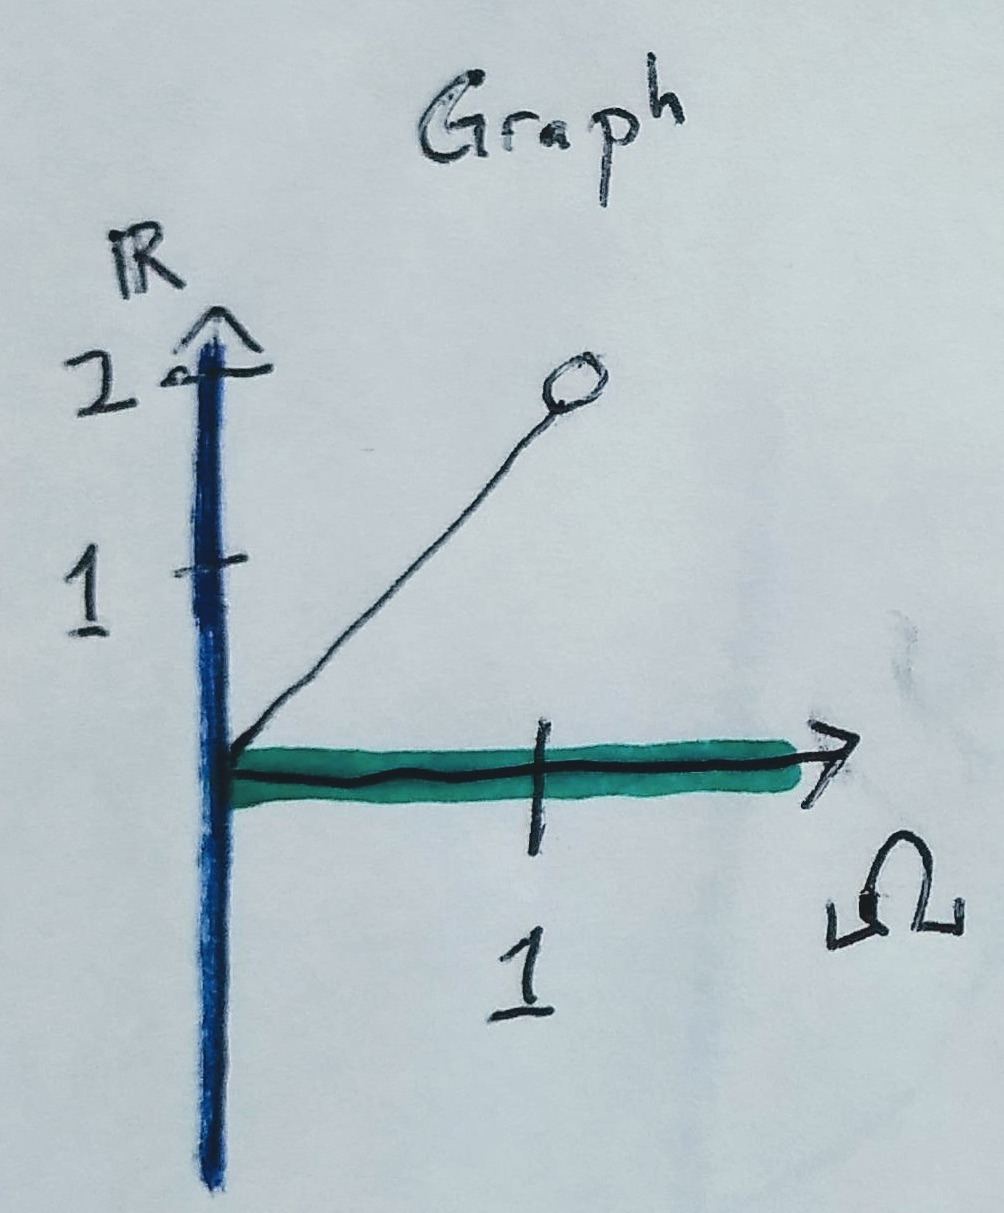
\includegraphics[width=0.3\linewidth]{figures/graph}
\end{center}


\subsection{The probabilist's event notation}\label{sec:probabilist}

It is tedious to write expressions like $X^{-1}(\{r \in \R : 6 \le r\})$. Probabilists noticed that the notation $(6 \le X)$ was not defined, and decided to give it a new, precise meaning: $X^{-1}(\{r \in \R : 6 \le r\})$. Some other examples:
\begin{itemize}
  \item $(X \in A) \defeq X^{-1}(A)$,
  \item $(X = x) \defeq X^{-1}(\{x\})$.
\end{itemize}
\begin{center}
	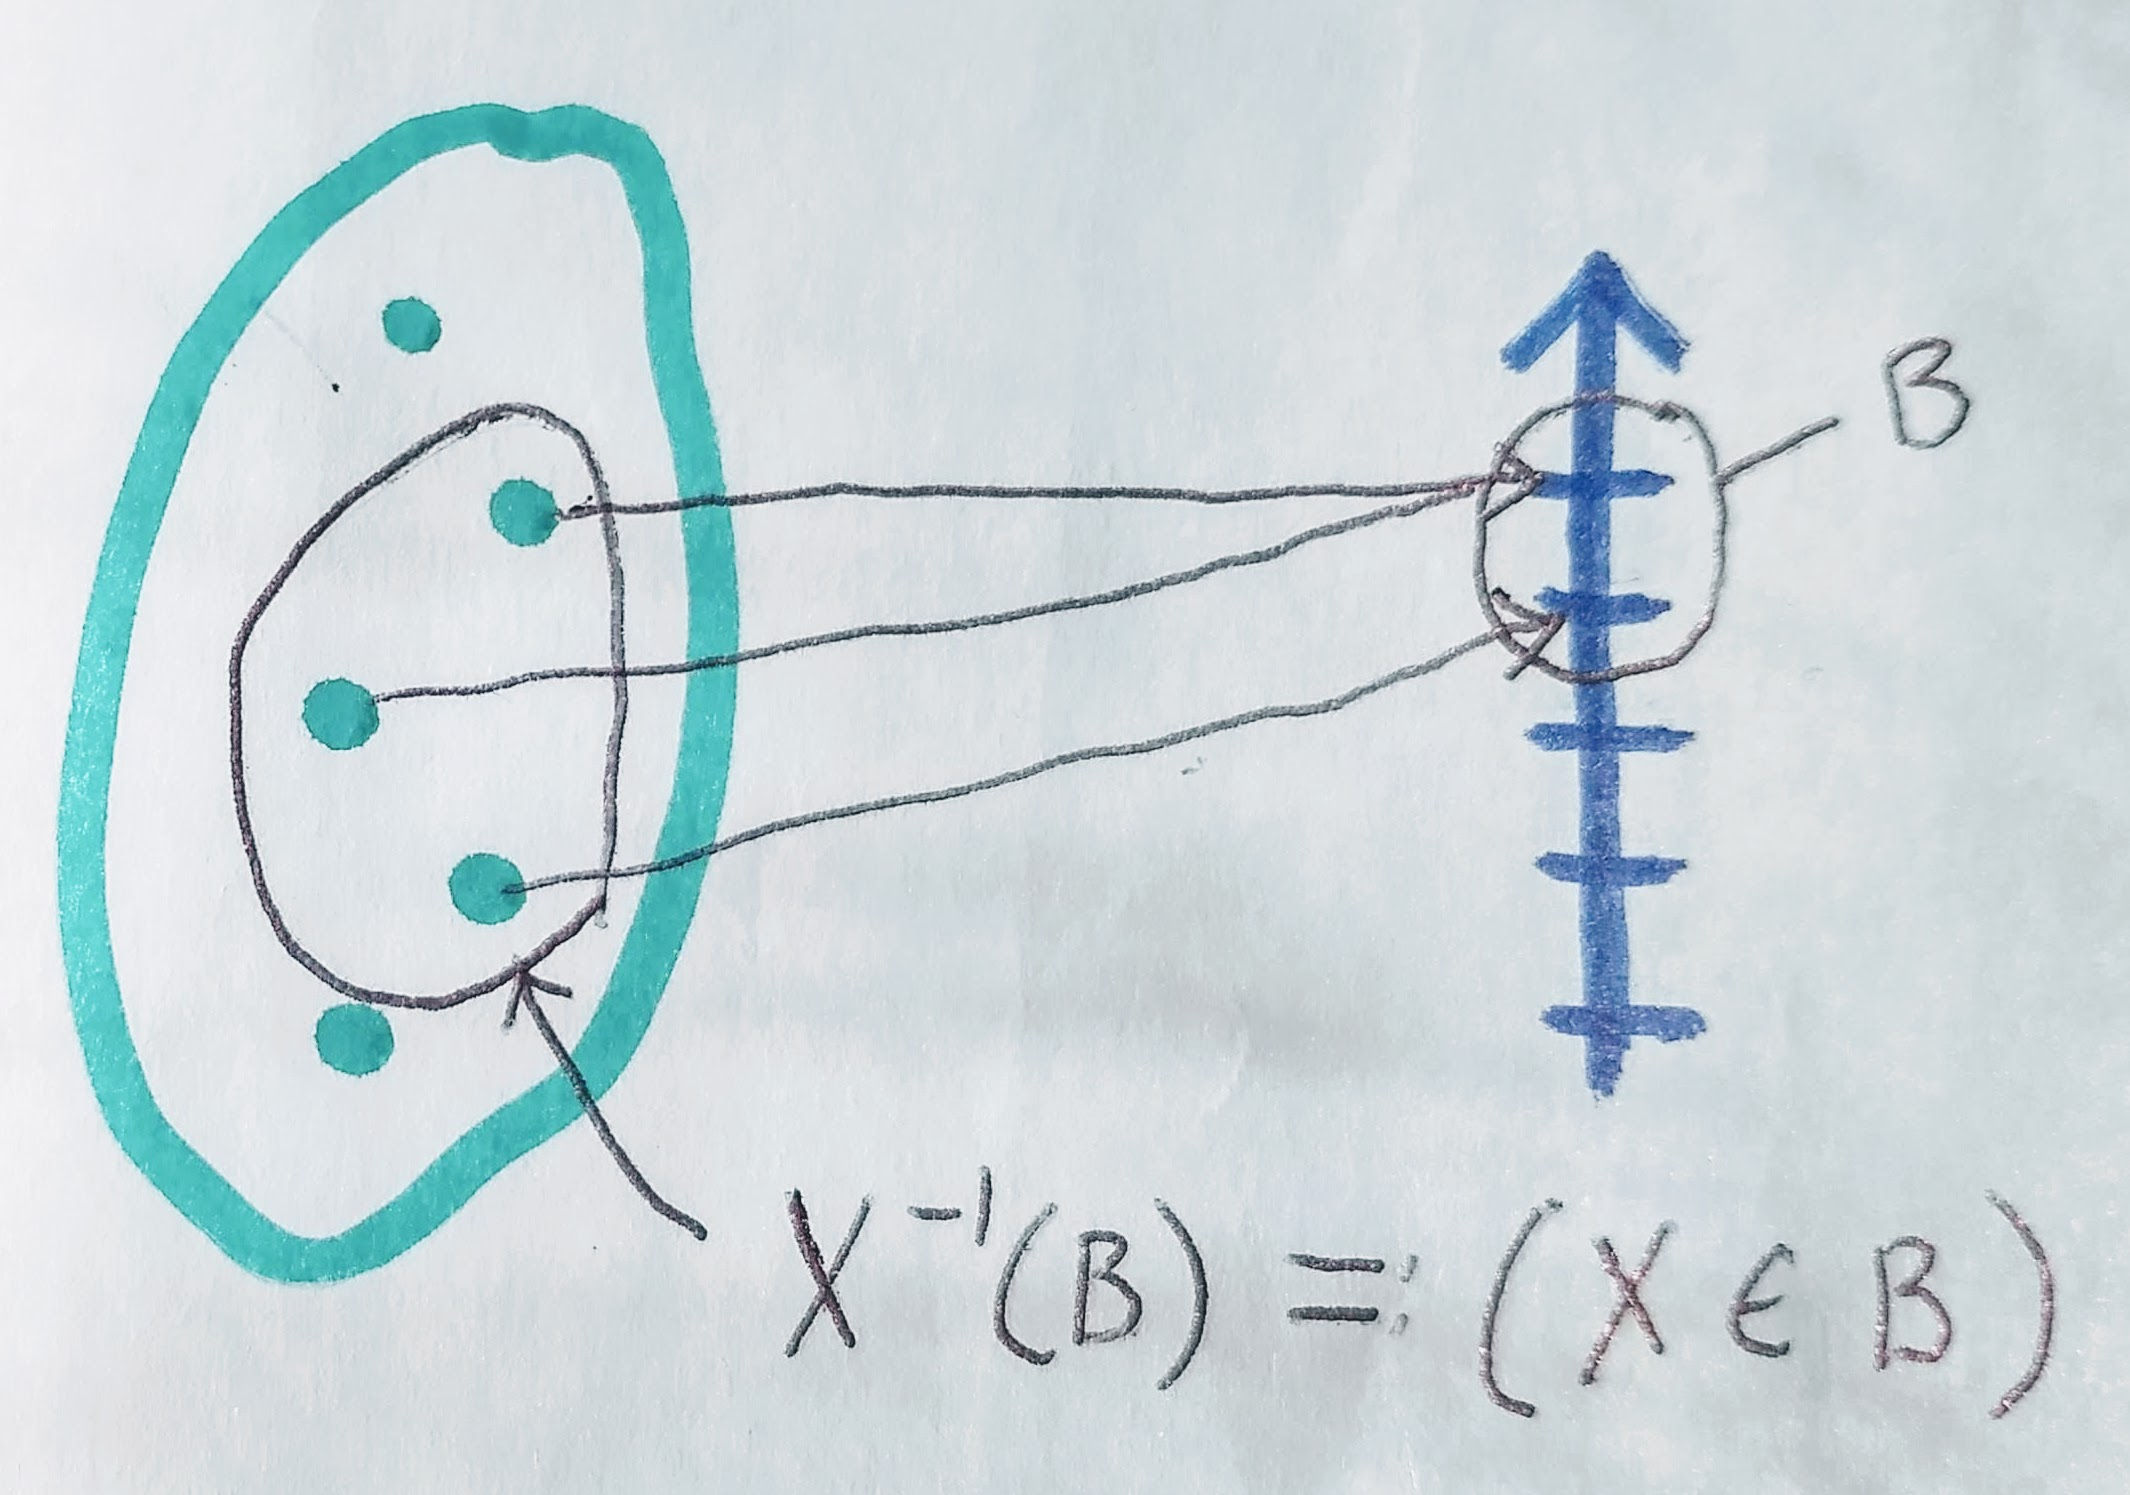
\includegraphics[width=0.5\linewidth]{figures/inverse}
\end{center}

\point{More generally:} \[(\text{logical statement }s\text{ containing a random variable }X) \defeq \{\omega \in \Omega : s(X(\omega))\text{ is true}\}. \]


\subsection{Constant random variables}

The simplest example of a random variable is a constant function, e.g. $X(\omega) = 42$ for all $\omega$ or $Y(\omega) = 3.14$ for all $\omega$, denoted $X = 42$ and $Y = 3.14$ respectively. These are boring but important building blocks. We will abuse notation and denote the random variables such as $X$ and $Y$ here by just $42$ and $3.14$ respectively. For example $Z + 3$ if a shorthand for the composition $g(Z, W)$, where $g(z, w) = z + w$ and $W(\omega) = 3$.

\subsection{Indicator random variables}\label{sec:indicator}

Often we need random variable taking binary values (either zero or one). These are called indicator random variables. 

For any set $A$, define the \emph{indicator function} or just indicator for short as follows: \[ \1_A(\omega) \defeq \1[\omega \in A] \defeq \bracearraycond{1 &\text{if }\omega\in A\\0&\text{otherwise.}} \]

The indicator random variable is just an indicator on an event.

If $A$ can be defined using the probabilist's notation introduced in Section~\ref{sec:probabilist}, for example if $A = (X = x)$, we will use the notation $\1(X = x)$ for $\1_A$.


\subsection{Modelling randomized algorithms as random variables}

\point{Recall:} we mentioned randomized algorithms as one of the motivations for learning Probability Theory. Randomized algorithms can be defined as algorithms having  access to the realization of one random variable. Since in practice we need several random variables, randomized algorithms use \emph{pseudo-random generators} to turn one random number into a potentially very large list of random variables. In this section we see how to model randomized algorithms and pseudo-random generators using random variables. 

\point{Example of a simple randomized algorithm:} which simulates 100 coin flips and counts the number of times the coin comes heads. More precisely, the algorithm takes as input a \emph{random seed} $r$ (an integer, but modelled in a computer as being in a finite range of values, from 1 and say $2^{32}$), and proceeds as follows:

\begin{enumerate}
	\item $s \gets 0$
	\item For $i = 1, 2, \dots, 100$:
	\begin{enumerate}
		\item Extract a pseudo-random coin flip from the least significant binary digit of $r$: \[x_i = r \mod 2.\]
		In other words, $x_i$ is equal to one if and only if $r$ is an odd number, otherwise it is equal to zero.
		\item increment the sum counter, $s \gets s + x_i$
		\item Get a new pseudo-random integer by ``flipping'' an artificial wheel of fortune (wheel because we do modular arithmetic modulo $m$, the number of slots in the wheel), first nudging it
		by a multiplicative amount $a$, then by a constant amount $c$:
		\[ r \gets (a r + c) \mod m.\]
	\end{enumerate}
	\item Return the sum $s$
\end{enumerate}

\point{Note:} Here, $m$, $a$ and $c$ are fixed constants. For example, the famous Numerical Recipes book \cite{press_numerical_2007} recommends $m = 2^{32}$, $a = 1664525$ and $c = 1013904223$.

\point{Illustration of how the flipping works:} from wikipedia, created by user Cmglee, distributed under CC BY-SA 3.0

\begin{center}
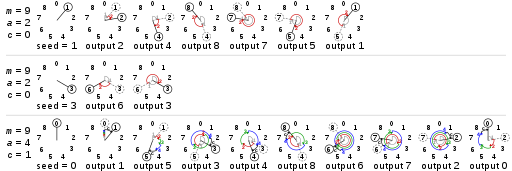
\includegraphics[width=0.9\linewidth]{figures/pseudo-random}
\end{center}

\point{Model for the algorithm?} Take $\Omega$ to be the set of integers $1, \dots, 2^{32}$. A seed corresponds to an outcome $\omega \in \Omega$. Given a seed, everything is deterministic in the algorithm. In particular, we can think about the value $x_1$ as the output of a deterministic function taking a seed as input. Let us call this function, $X_1 : \Omega \to \{0, 1\}$, and as our choice of letter suggest, it is indeed a random variable. Similarly, we can define random variables $X_2, X_3, \dots, X_{100}$, each one being a deterministic function (of increasing complexity) of the input random seed $\omega$. E.g.:
\[ X_2(\omega) = ((a\omega + c) \mod m) \mod 2. \]

\point{Practical importance.} This model illustrates a key design pattern useful when building any randomized algorithm: 
\begin{itemize}
	\item Make the random seed an explicit input of the program.
	\item Given this input, all computations should be deterministic.
\end{itemize}
This is useful because you can re-run exactly the same program, i.e. \emph{reproduce your results}. This comes handy if there is a bug you need to fix and you want to replay the crash to analyze in detail what happened. It is also handy if someone wants to replicate somebody else's published work.  

\point{Better pseudo-random generators:} the recipe used here ($r \gets (ar + c) \mod m$) is called a \emph{linear congruential generator}. This class of generators have been largely superseded by other methods, a good choice for example is the Mersenne Twister pseudo-random generator \cite{matsumoto_mersenne_1998}.


\subsection{Distribution of a random variable}\label{sec:distribution}

\point{Idea:} you give me a probability space $(\Omega, \events, \P)$ and a random variable $X : \Omega \to \states$, and I create a new probability $\P'$. This new probability is defined on the values $\states$ that the random variable takes.

\point{Definition:} for any $B \in \events_\states$, set $\P'(B) \defeq \P(X \in B)$.
\begin{center}
	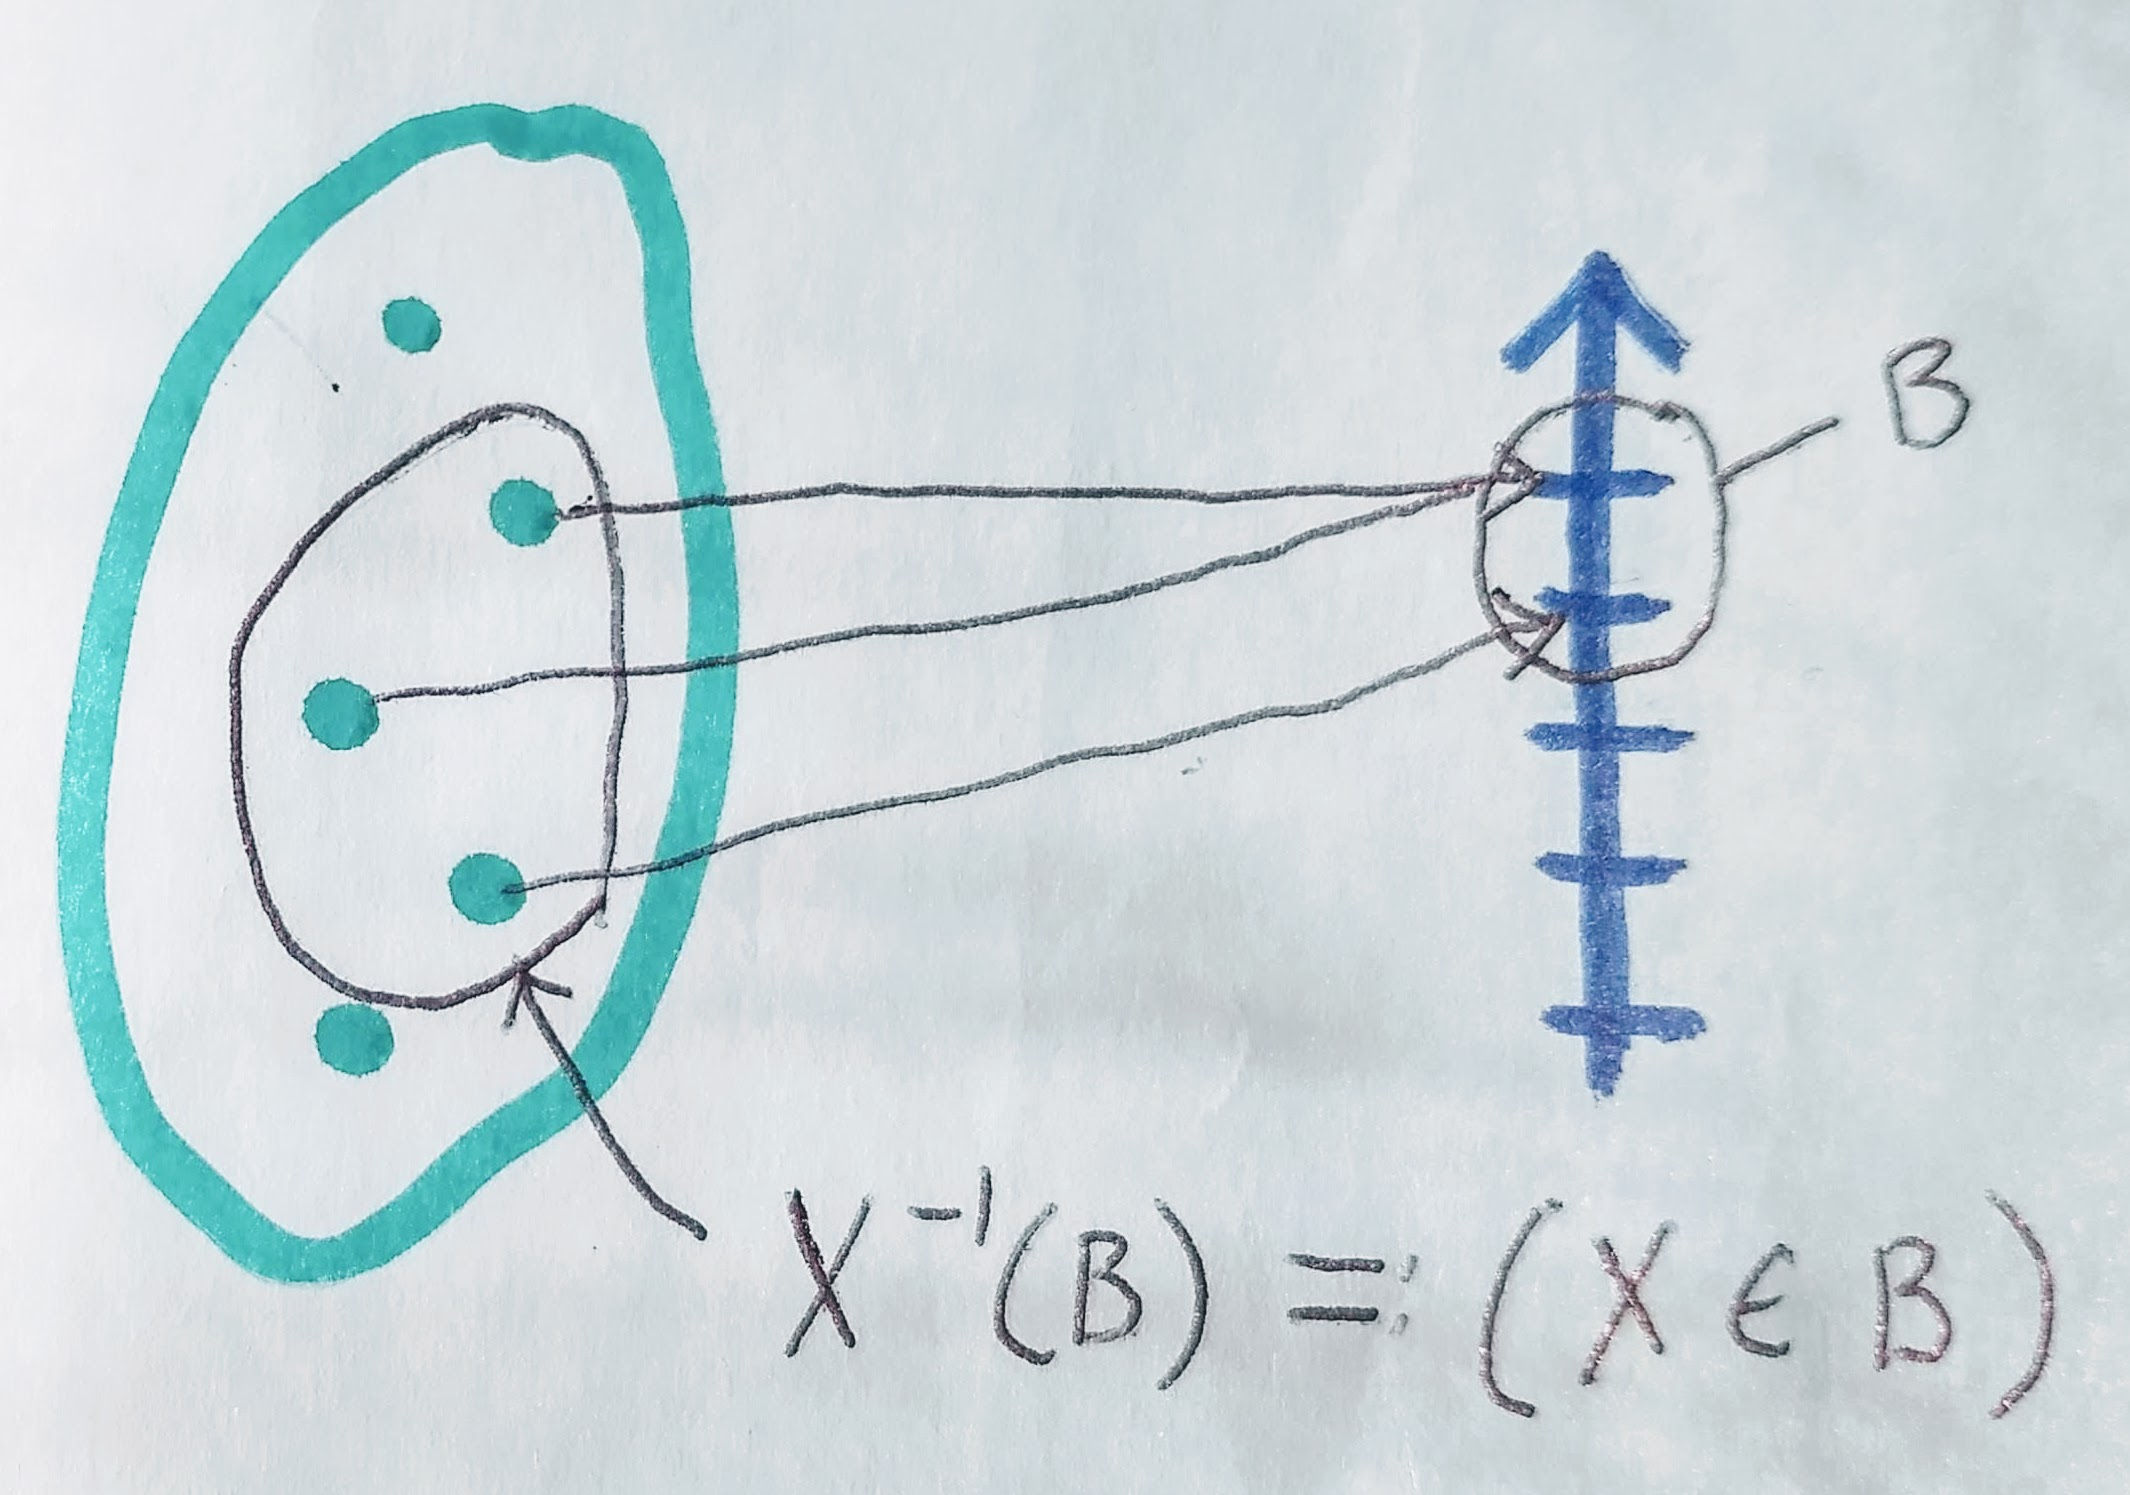
\includegraphics[width=0.5\linewidth]{figures/inverse}
\end{center}

\point{Notation:} we denote this new probability $\P'$ by $\P_X$, and call it the \emph{distribution of $X$}.

\point{Exercise:} suppose $X$ is an indicator variable on an event $A$, with $p = \P(A)$. Find the distribution of $X$. The answer is called ``Bernoulli with parameter $p$'', denoted $\P_X = \Bern(p)$. The shorthand $X \sim \Bern(p)$ is also widely used in statistics. 

\point{Possible confusion:} ``probability distribution'' is a synonym of ``probability measure.'' Here we defined the ``distribution \emph{of} $X$,'' which is a specific way of constructing a probability measure.


\subsection{Cumulative distribution function}

\point{Idea:} a probability is a function taking inputs from a tricky space ($\events$). This makes it hard to plot naively. It would be nice to be able to summarize it with a function taking inputs in a more familiar space, $\R$.

\point{Note:} the following definition only works for $\states = \R$.

\point{Definition:} the \CDF\ of a random variable is given for all $x \in \R$ by: \[ F_X(x) \defeq \P(X \le x). \]
\begin{center}
	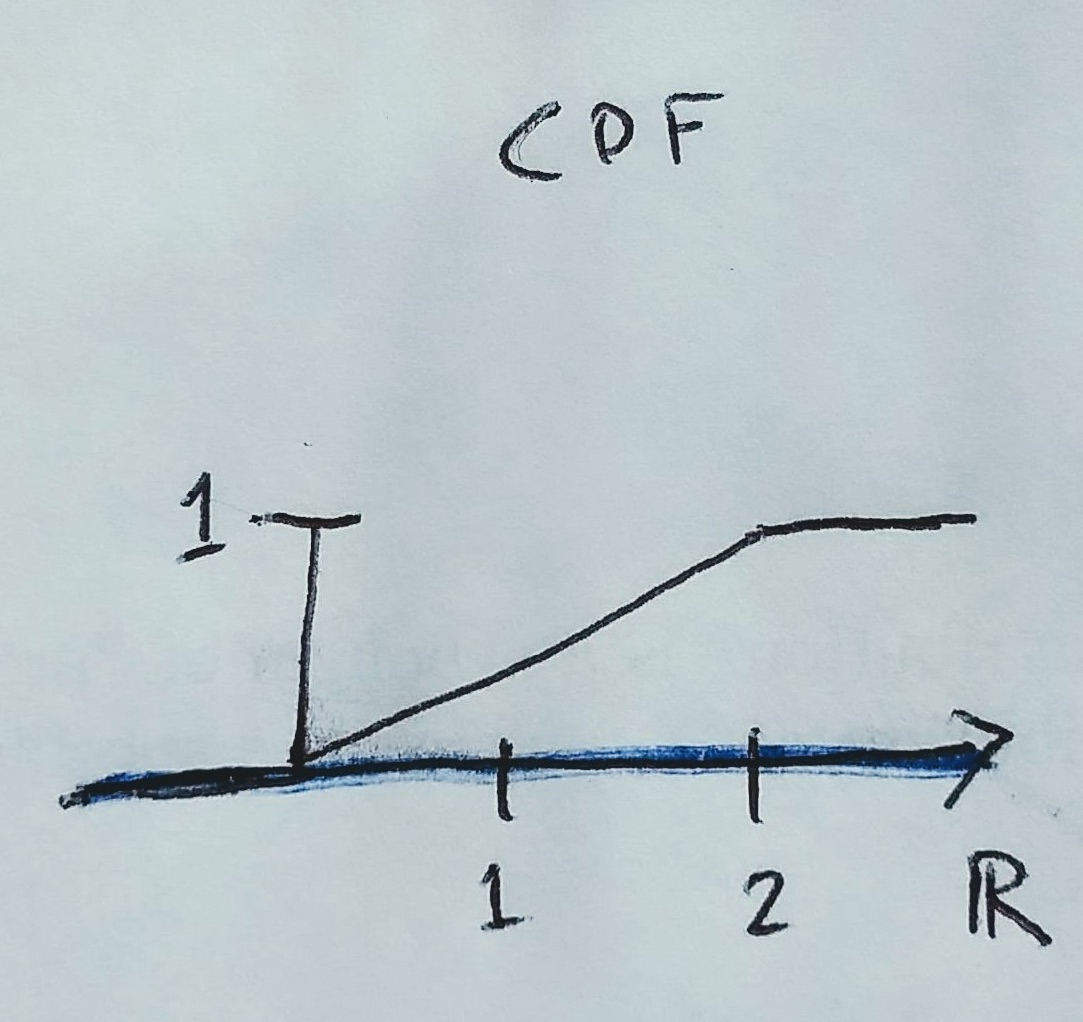
\includegraphics[width=0.3\linewidth]{figures/cdf}
\end{center}

\point{Exercise:} this is the same as $\P_X((-\infty, x])$.


\subsection{Equality in distribution}\label{sec:equal-in-distribution}

\point{Example:} Suppose the only probability distribution available in some programming language is the uniform distribution on $[0, 1)$. How can we transform it into a coin toss?

\point{An answer:} $X_1 = \1_{[0, 1/2)}$.

\point{Question:} is this answer unique? No! For example, $X_2 = \1_{[0, 1/4)} + \1_{[1/2, 3/4)}$ will also do!
\begin{center}
	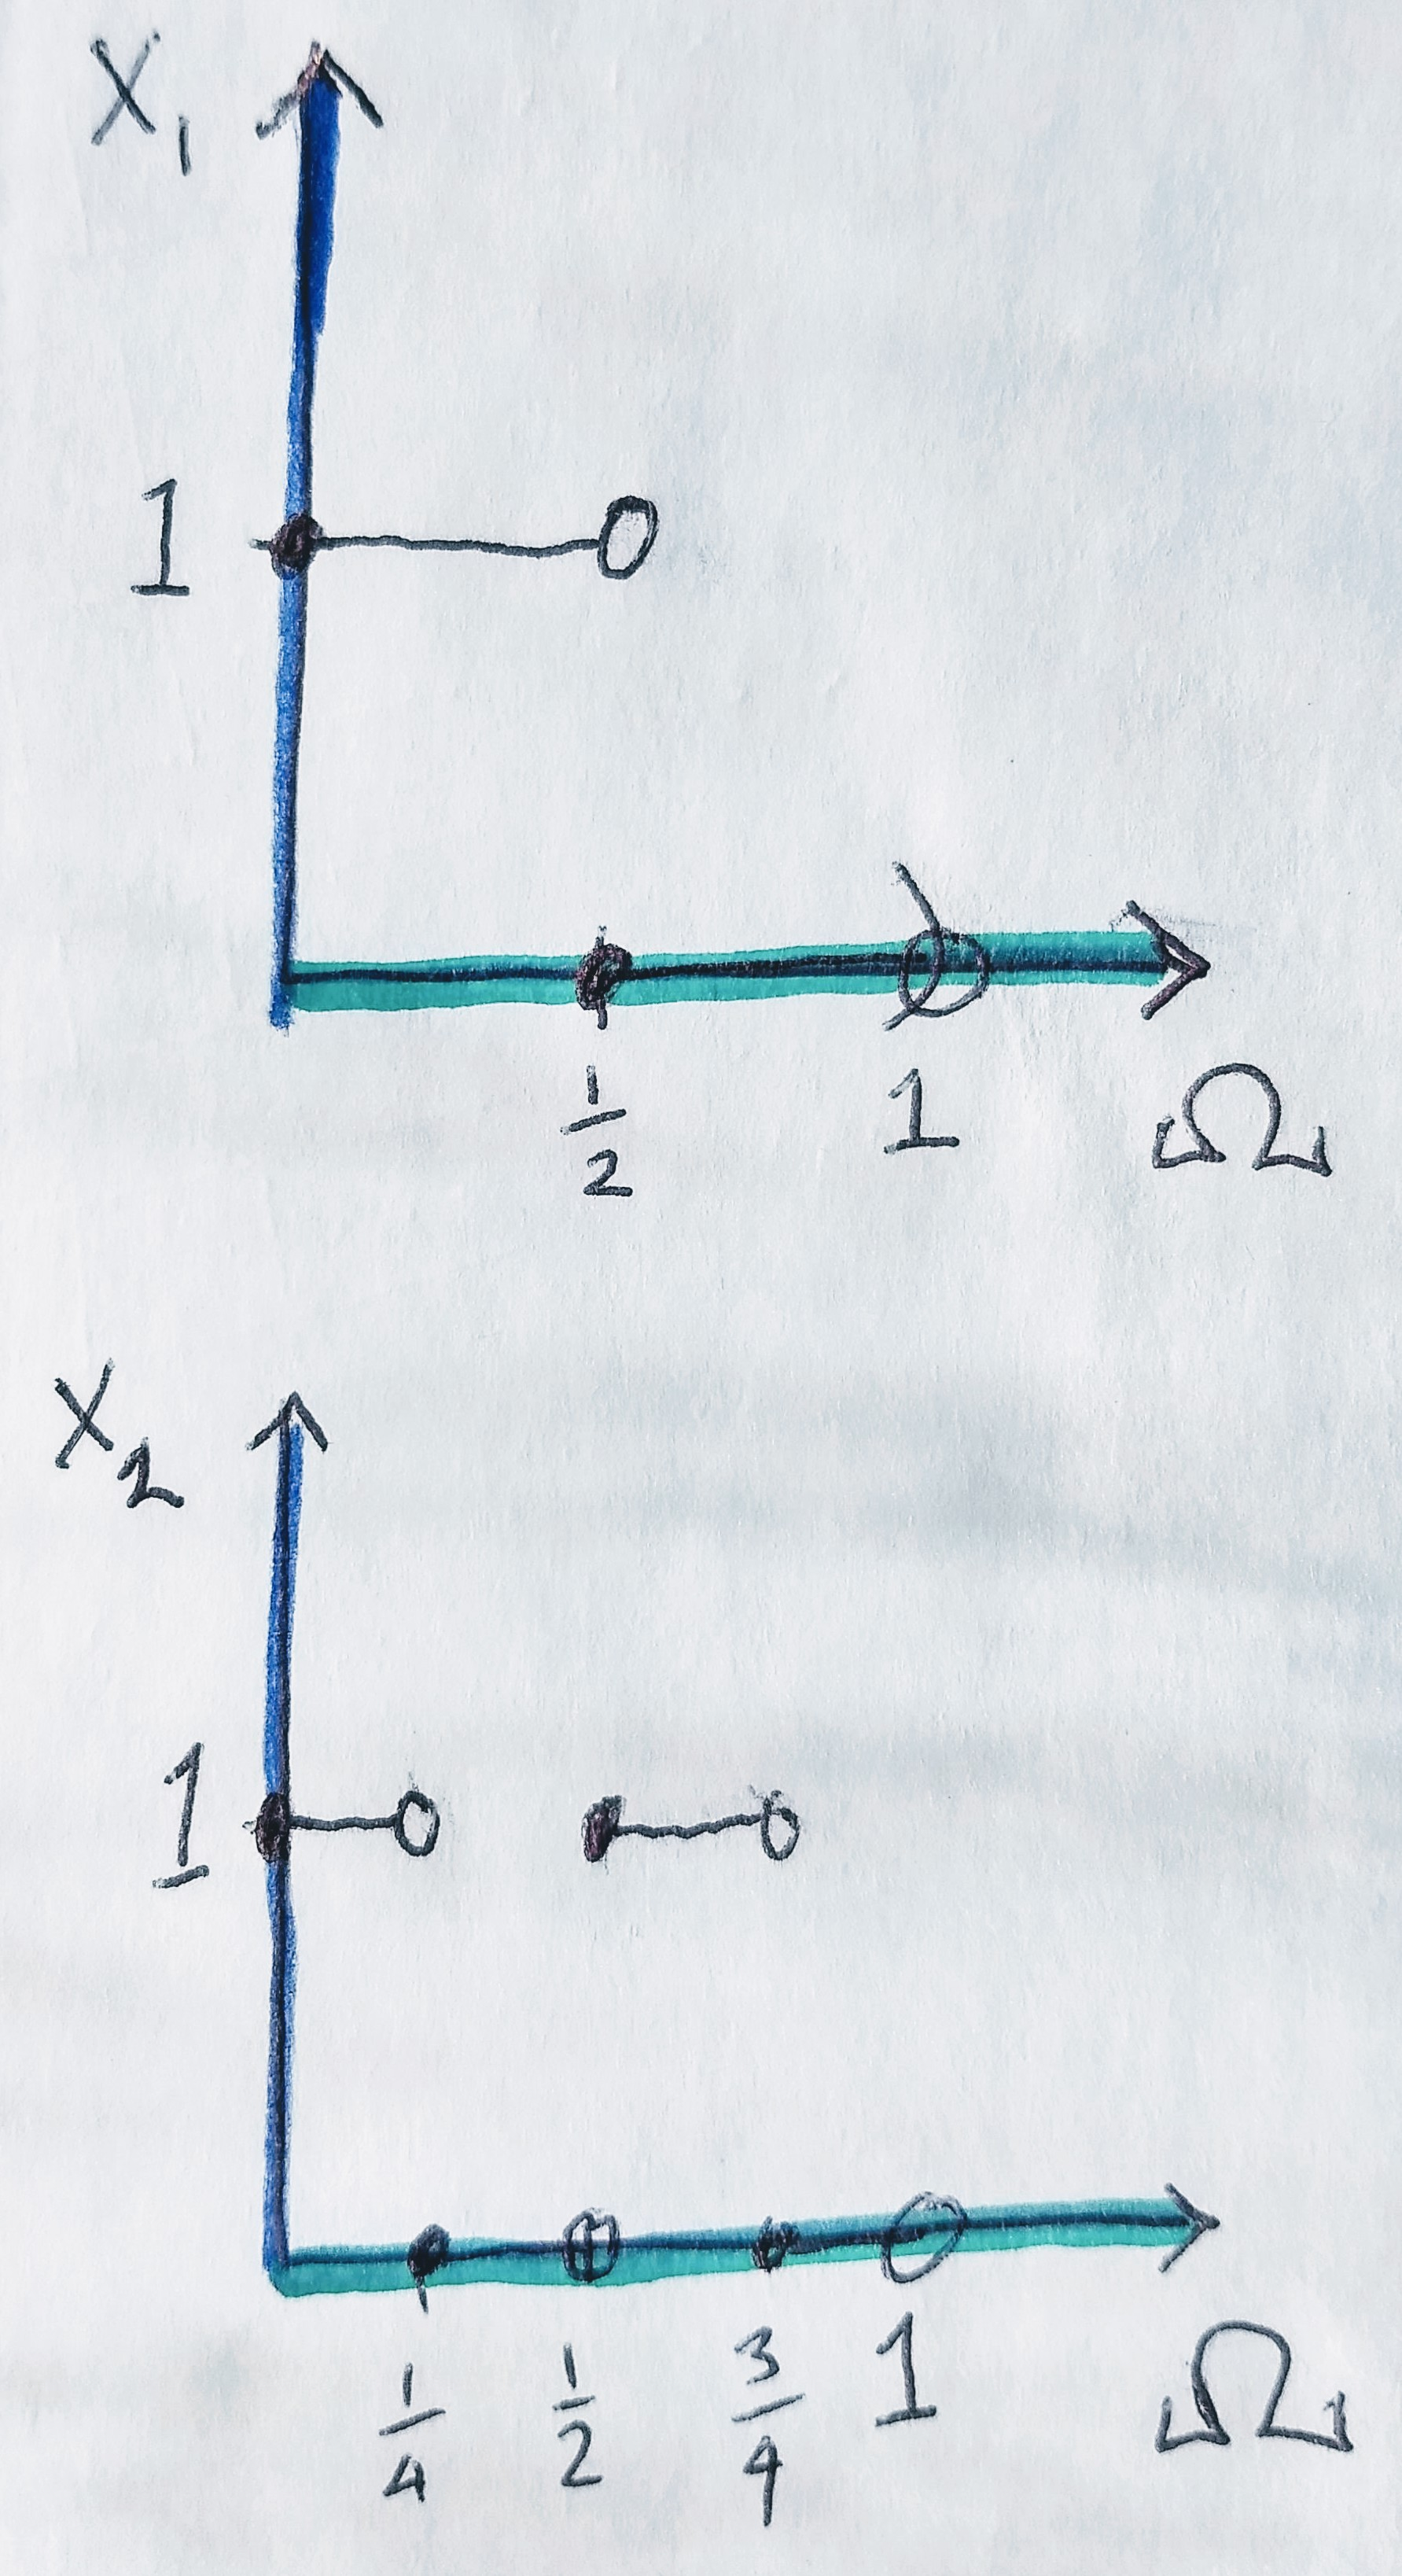
\includegraphics[width=0.3\linewidth]{figures/eq-dist}
\end{center}

\point{Note:} 
\begin{enumerate}
  \item $X_1 \neq X_2$ (the two functions are not equal, for example $X_1(1/4) = 1 \neq 0 = X_2(1/4)$
  \item \label{item:dist} but: $\P_{X_1} = \P_{X_2}$.
\end{enumerate}

\point{Definition:} We call \ref{item:dist} \emph{equality in distribution}, denoted $X_1 \deq X_2$. 


\subsection{Densities (first definition)}\label{sec:density-first-def}

A random variable is said to have \emph{density} $f \ge 0$ if: \[ F_X(x) = \int_{-\infty}^x f(z) \ud z. \] Note that we will cover a more general definition of density later in this course.

\point{Example:} a density for the exponential distribution is given by \[ f(x) = \1[x \ge 0] \lambda e^{-x\lambda}. \]

\point{Exercise:} find an example where there is a $x$ such that a density has $f(x) > 1$.


\subsection{Limit properties of probability measures}\label{sec:limit-pr-measures}

\point{Lemma: monotonicity.} If $B \subset A$ are events, then $\P(B) \le \P(A)$.

\point{Proof idea:} Use the ``donut decomposition,'' $A = B \sqcup (A \backslash B)$, where we use the symbol $\sqcup$ to denote a union while asserting that the two sets we are taking the union over are disjoint.
\begin{center}
	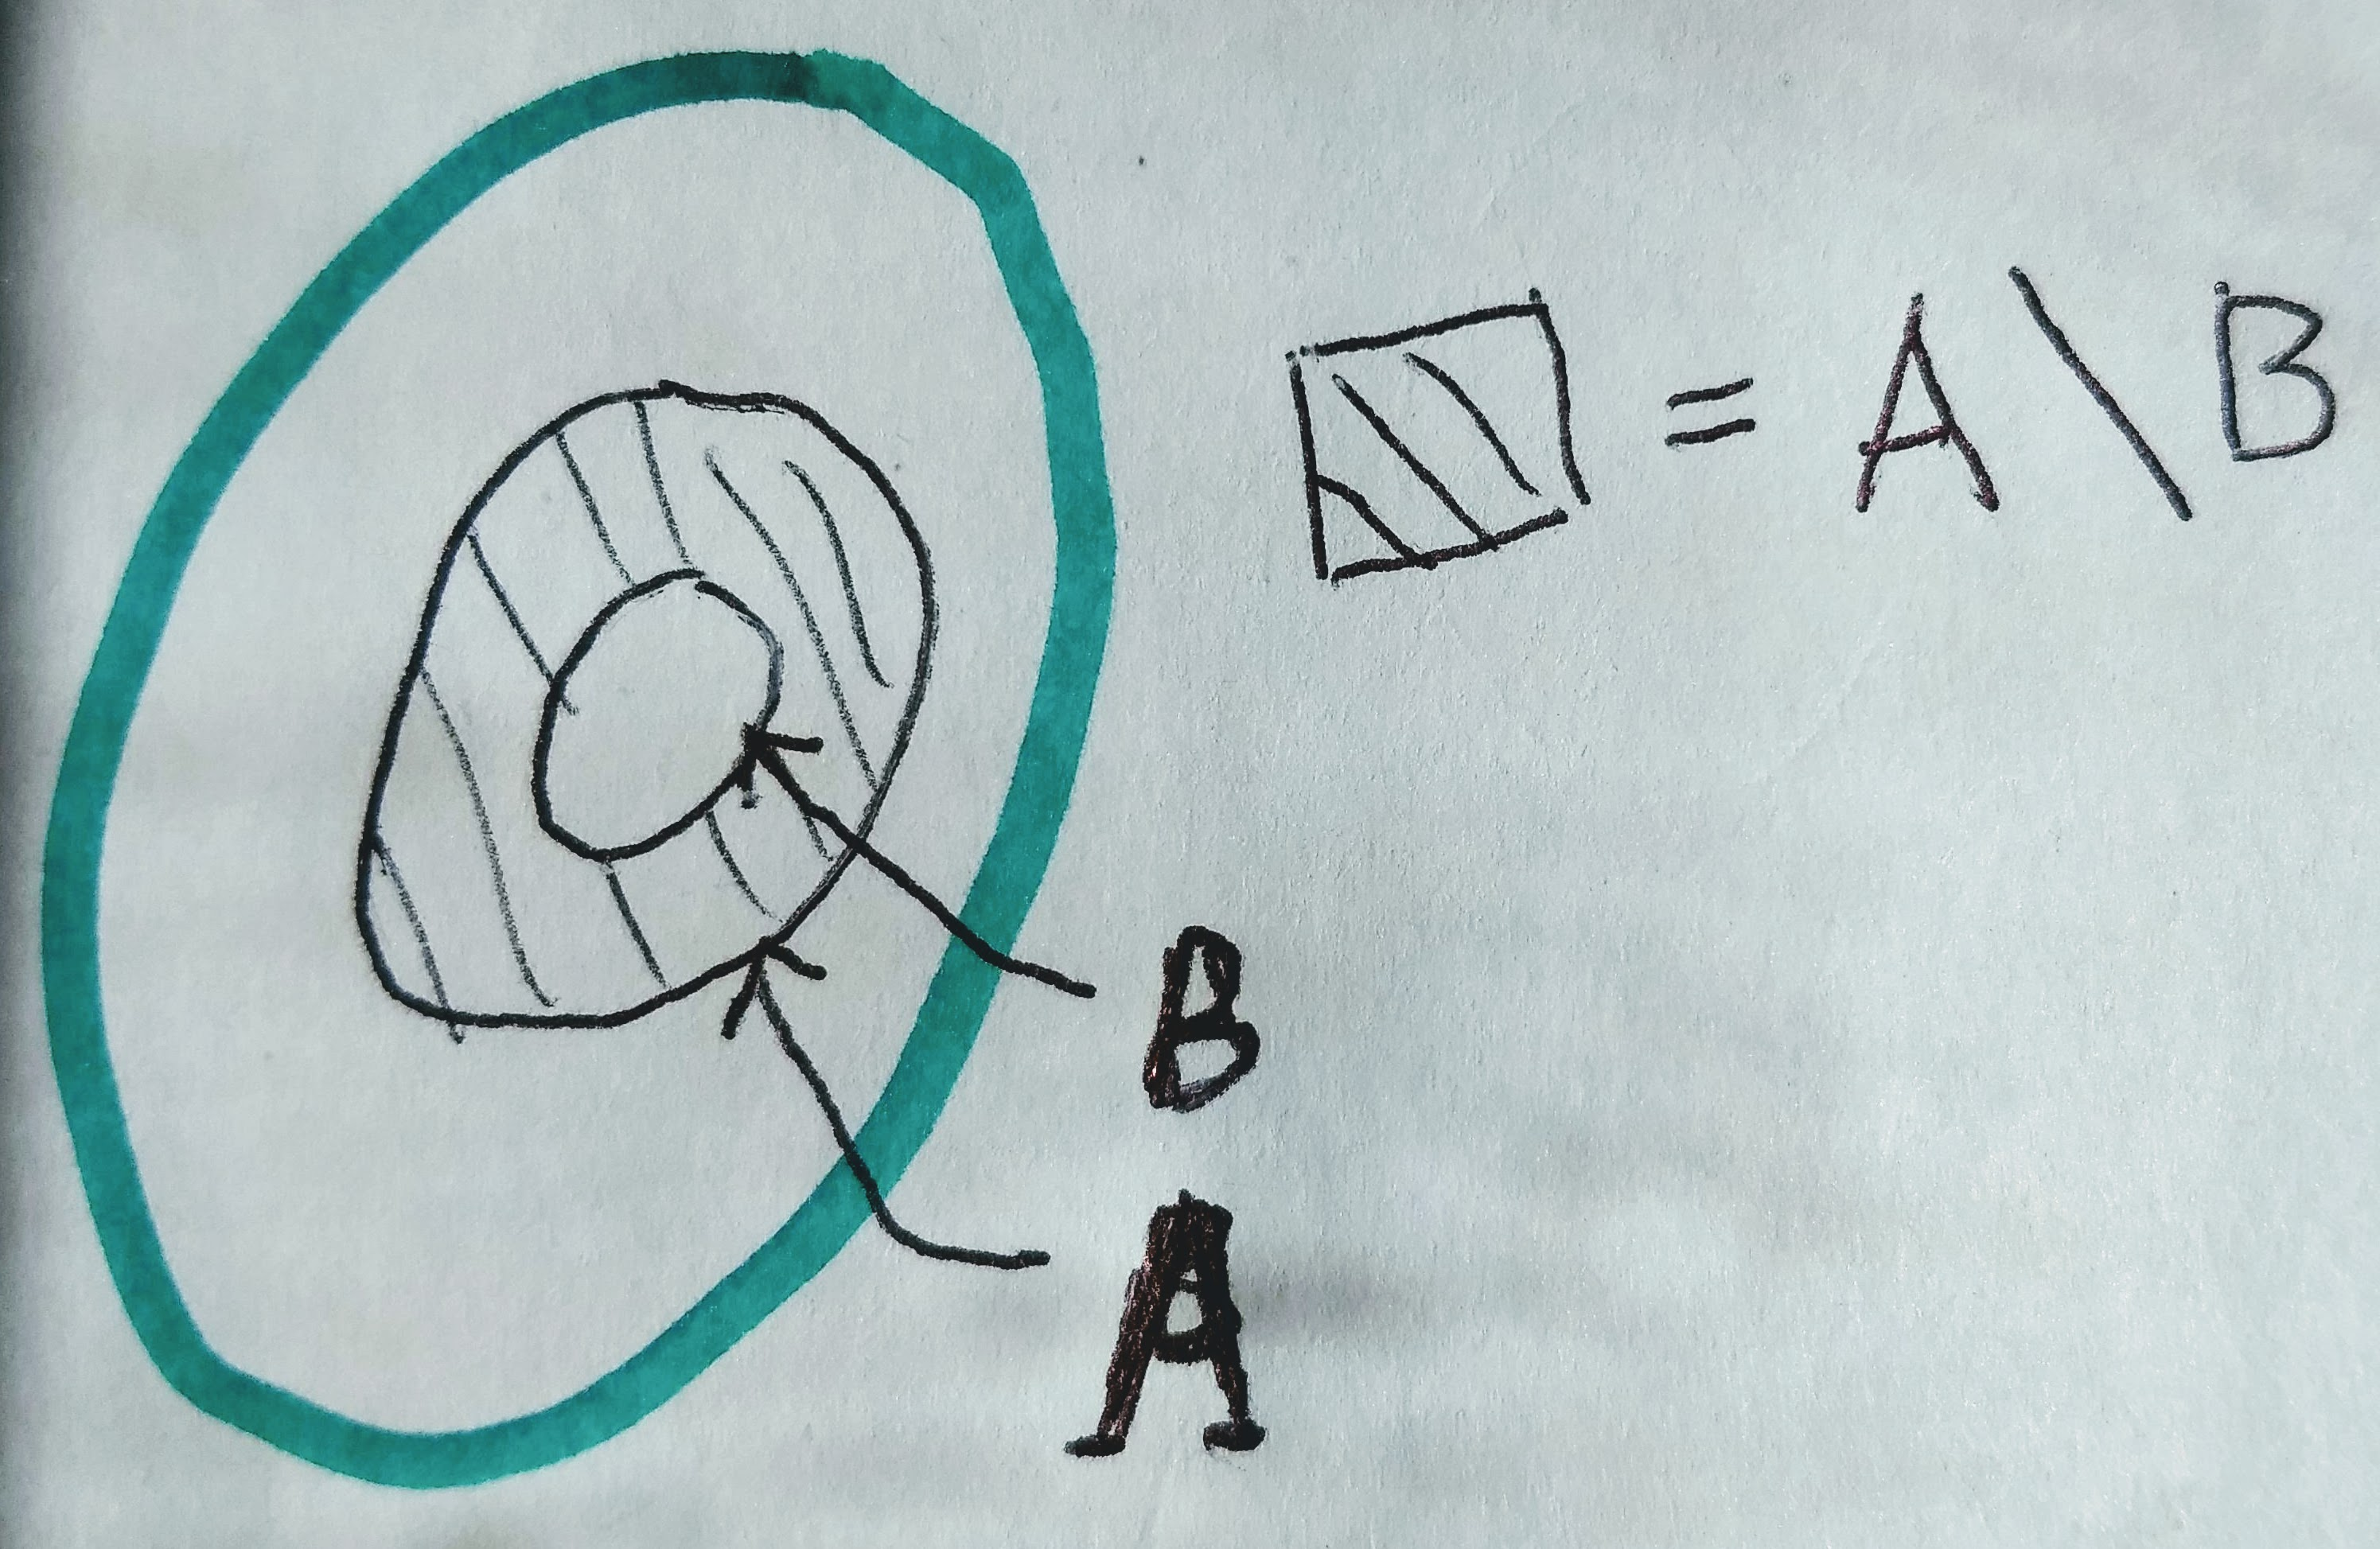
\includegraphics[width=0.3\linewidth]{figures/donut-1}
\end{center}

\point{Notation:} to express the following limit properties, we make use of the following overloaded notations,
\begin{itemize}
  \item Monotone real numbers limits:
  \begin{itemize}
    \item If $r_1 \le r_2 \le \dots$, and $\lim r_i = r$, we write $r_i \uparrow r$,
    \item If $r_1 \ge r_2 \ge \dots$, and $\lim r_i = r$, we write $r_i \downarrow r$.
  \end{itemize}
  \item Monotone set limits:
  \begin{itemize}
    \item If $A_1 \subset A_2 \subset \cdots$, and $\cup A_i = A$, we write $A_i \uparrow A$,
    \item If $A_1 \supset A_2 \supset \cdots$, and $\cap A_i = A$, we write $A_i \downarrow A$.
  \end{itemize}
\end{itemize}

\point{Monotonicity of probability measures:} 
\begin{itemize}
  \item $A_i \uparrow A \Longrightarrow \P(A_i) \uparrow \P(A)$,
  \item $A_i \downarrow A \Longrightarrow \P(A_i) \downarrow \P(A)$.
\end{itemize}

\point{Proof idea for the increasing case:} generalize the donut decomposition and write 
\[ A = A_1 \sqcup (A_2 \backslash A_1) \sqcup (A_3 \backslash A_2) \sqcup \cdots, \]
then use countable additivity to get:
\[ \P(A) = \P(A_1) + \lim_{n \to \infty} \sum_{i=1}^n \P(A_{i+1} \backslash A_i), \]
using our previous monotonicity property, and telescoping the sum inside the limit, we get:
\[ \P(A) = \P(A_1) + \lim_{n \to \infty} [\P(A_n) - \P(A_1)] = \lim_{n\to\infty} \P(A_n). \]


\subsection{Limit properties of CDFs}\label{sec:limit-properties-cdfs}

Since the \CDF\ is derived from a probability measure, it shares similar continuity property. But being a function from the real to $[0,1]$, these monotonicity properties coincide with familiar notions from elementary real analysis. 

\point{Notation:} Throughout this section, $F$ denotes the \CDF\ of some random variable $X$, $F \defeq F_X$.

\point{Monotonicity of \CDFs:} $x \le y \Longrightarrow F(x) \le F(y)$ ($F$ is monotone increasing).

\point{Proof:} $x \le y \Longrightarrow (X \le x) \subset (X \le y)$, so we can use monotonicity of the probability measure $\P$ to conclude the proof.
\begin{center}
	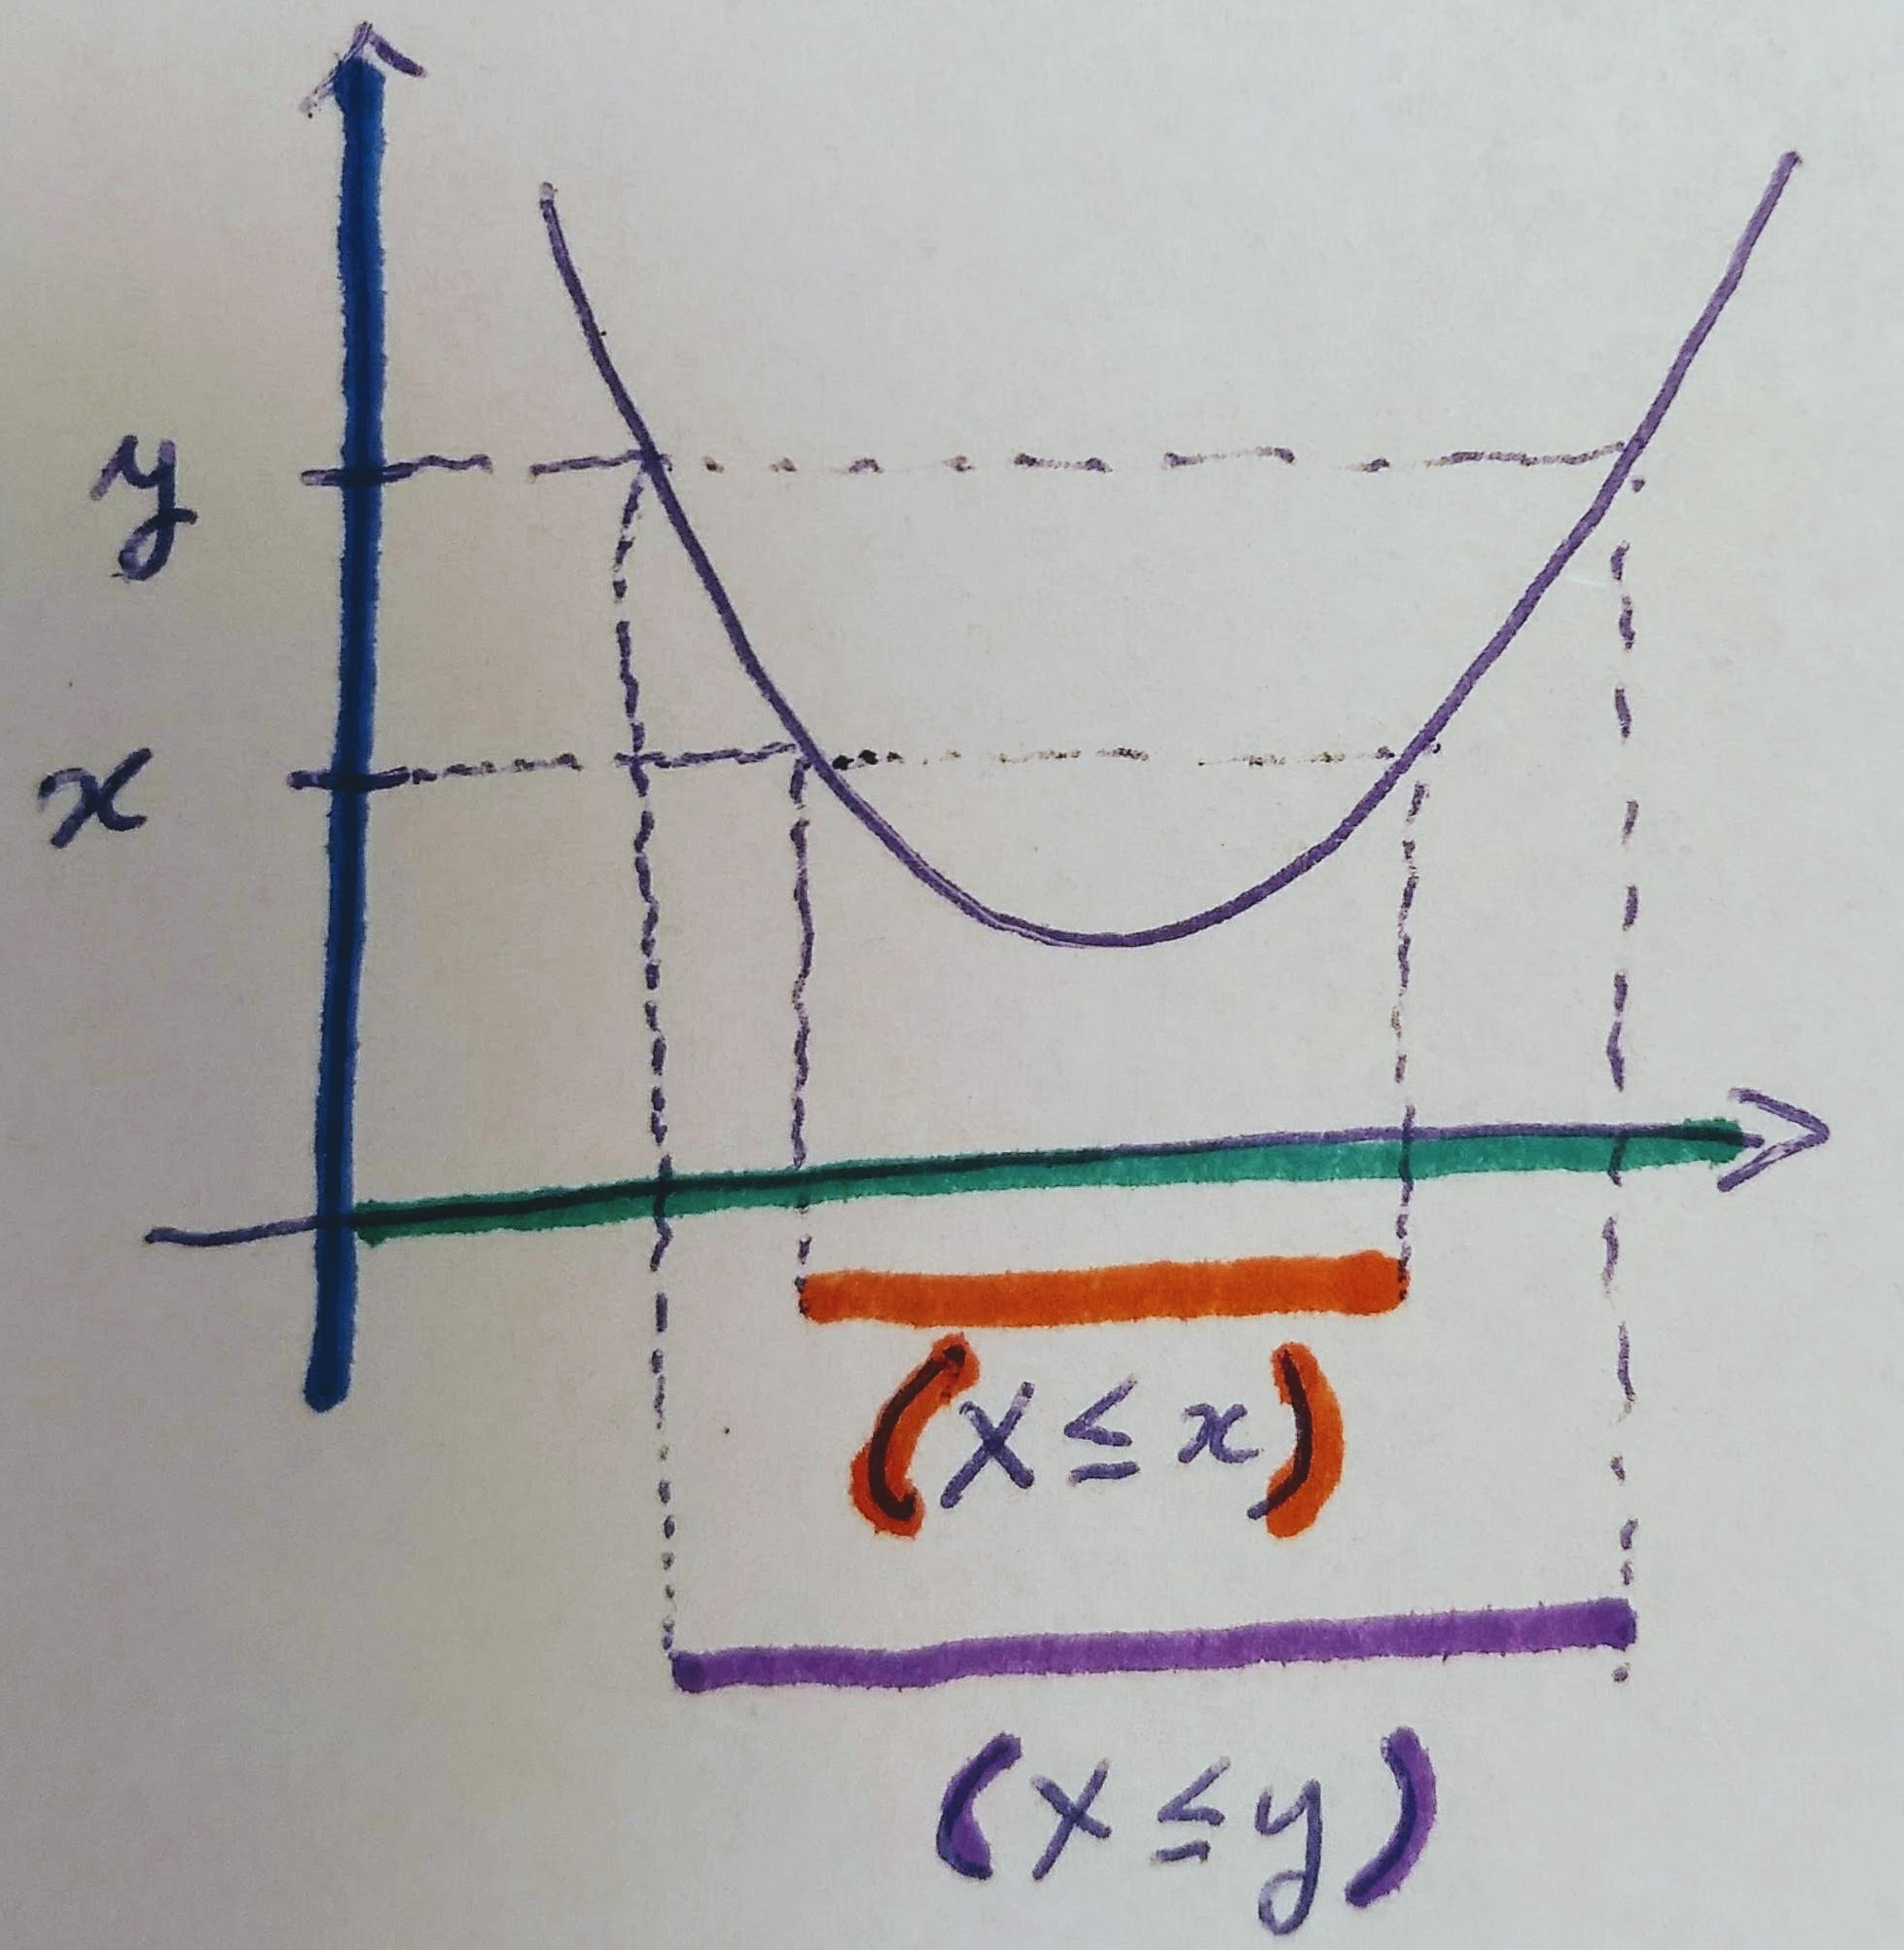
\includegraphics[width=0.3\linewidth]{figures/inclusion}
\end{center}

\point{Semi-continuity property:} 
\begin{enumerate}
  \item \label{item:cont1} $x_i \uparrow x \Longrightarrow$ the limit $\lim F(x_i)$ exists,
  \item \label{item:cont2} $x_i \downarrow x \Longrightarrow F(x_i) \downarrow F(x)$.
\end{enumerate}

\point{Proof idea for the decreasing case:} we have $(X \le x_i) \supset (X \le x_{i+1})$, so by monotonicity of $\P$, we get, for $A_i = (X \le x_i)$,
\[ F(x_i) = \P(A_i) \downarrow \P(\cap A_i), \]
where $\cap A_i = (X \le x)$ (see figure below), therefore $\P(\cap A_i) = F(x)$.
\begin{center}
	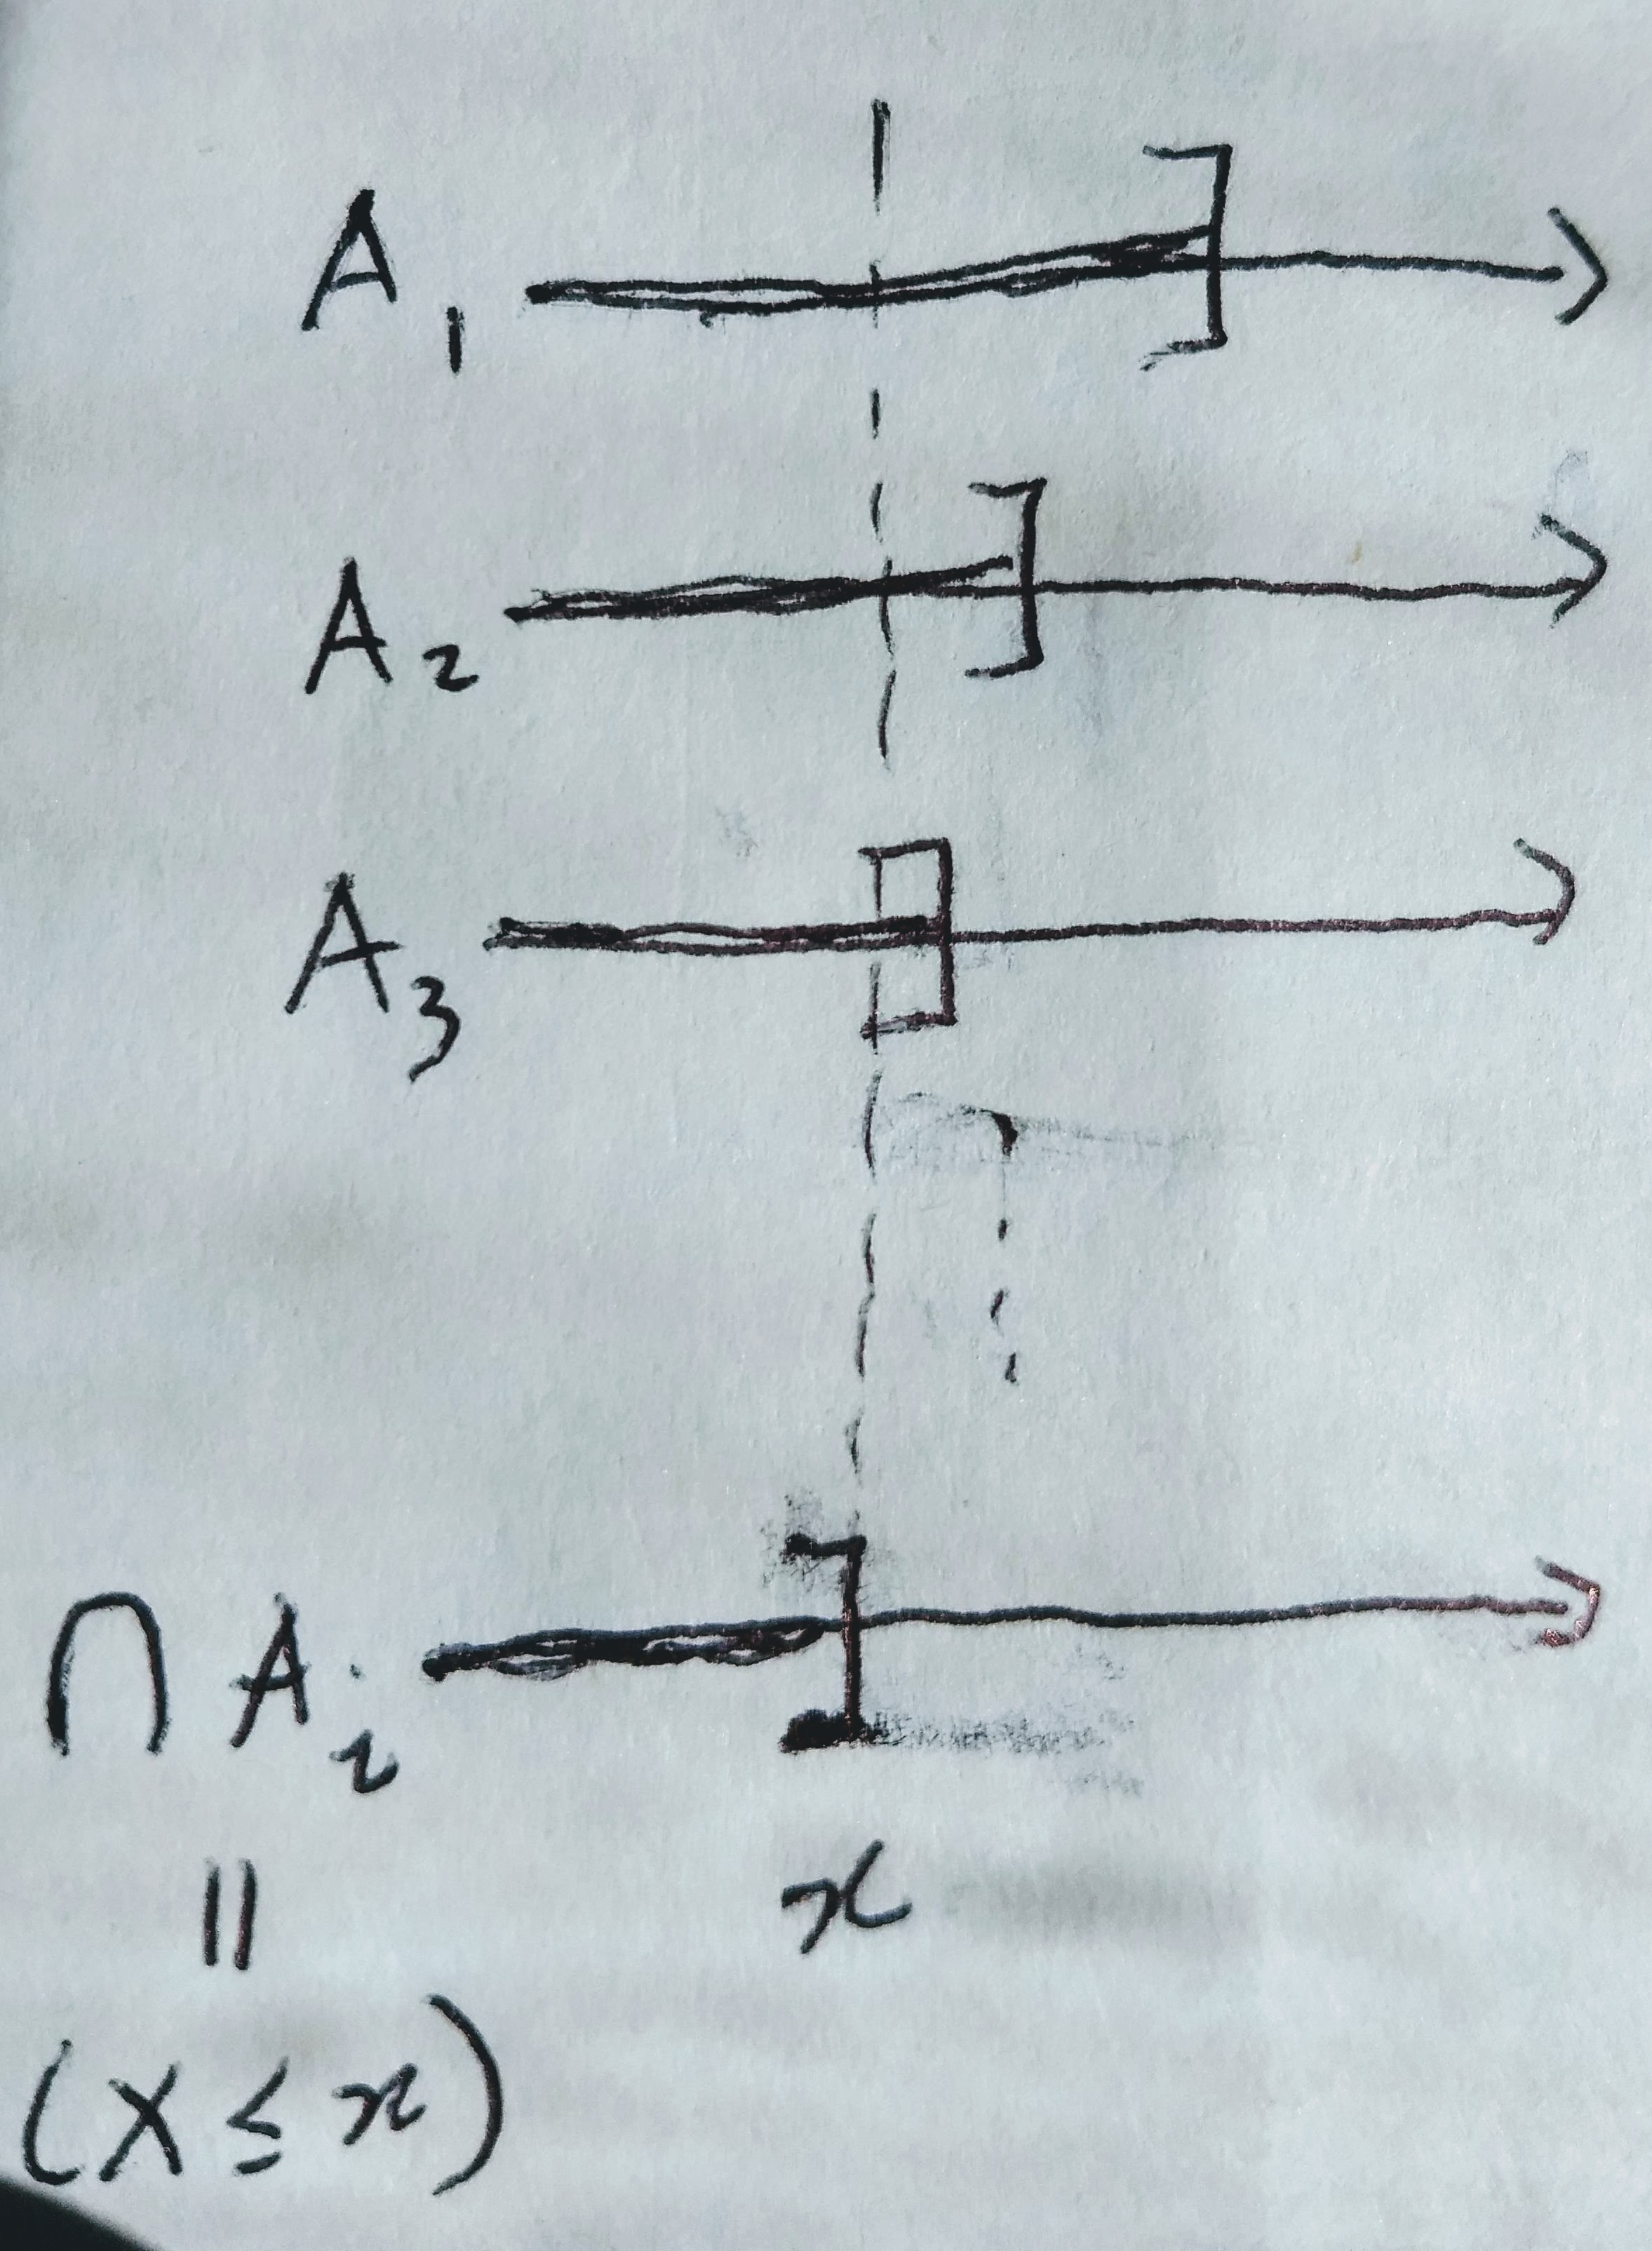
\includegraphics[width=0.3\linewidth]{figures/limit-cdf}
\end{center}

\point{Reason:} for the asymmetry between semi-continuity property \ref{item:cont1} and \ref{item:cont2}. First, do the proof for the increasing case as an exercise. You will see that in the increasing case, the limit of the probabilities is given by $\P(X < x)$, which is not guaranteed in general to be equal to $F(x)$ (because of a potential point mass as $x$).

\point{Terminology:} functions that satisfy the semi-continuity properties (\ref{item:cont1} and \ref{item:cont2}) are called cadlag, coming from ``continue \`a droite, limite \`a gauche'' (French for ``continuous to the right, limits to the left'').

\point{Proposition:} let $F : \R \to [0, 1]$ be some function. The following are equivalent:
\begin{enumerate}
  \item \label{item:inv-cdf-eq1} The function $F$ is non-decreasing, cadlag and satisfies the boundary conditions $\lim_{x \to -\infty} F(x) = 0$ and $\lim_{x \to +\infty} F(x) = 1$ (denoted $F(-\infty) = 0$ and $F(+\infty) = 1$),
  \item \label{item:inv-cdf-eq2} There is some random variable $X$ with $F_X = F$.
\end{enumerate}

\point{Proof idea:} we proved the main steps of \ref{item:inv-cdf-eq1}$\Longleftarrow$\ref{item:inv-cdf-eq2}. The main idea for the other direction is to use the following construction:
\[ X(\omega) \defeq \sup\{x : F(x) < \omega\}. \]

\point{Note:} this is a first instance of an important idea in this course, namely to identify the distributions of random variables with simpler types of functions.


\subsection{Building random variables with a prescribed CDF}\label{sec:inverse-cdf}

\point{Example/exercise:} simulate an exponential random variable (defined below) from a uniform distribution on $[0, 1)$, where an exponential random variable is defined as follows:

\point{Definition:} we say $X$ is a standard exponential random variable, a statement denoted $X \sim \text{Exp}(\lambda)$, if \[F_X(x) = \1[x \ge 0] (1 - e^{-x \lambda}). \]
\begin{center}
	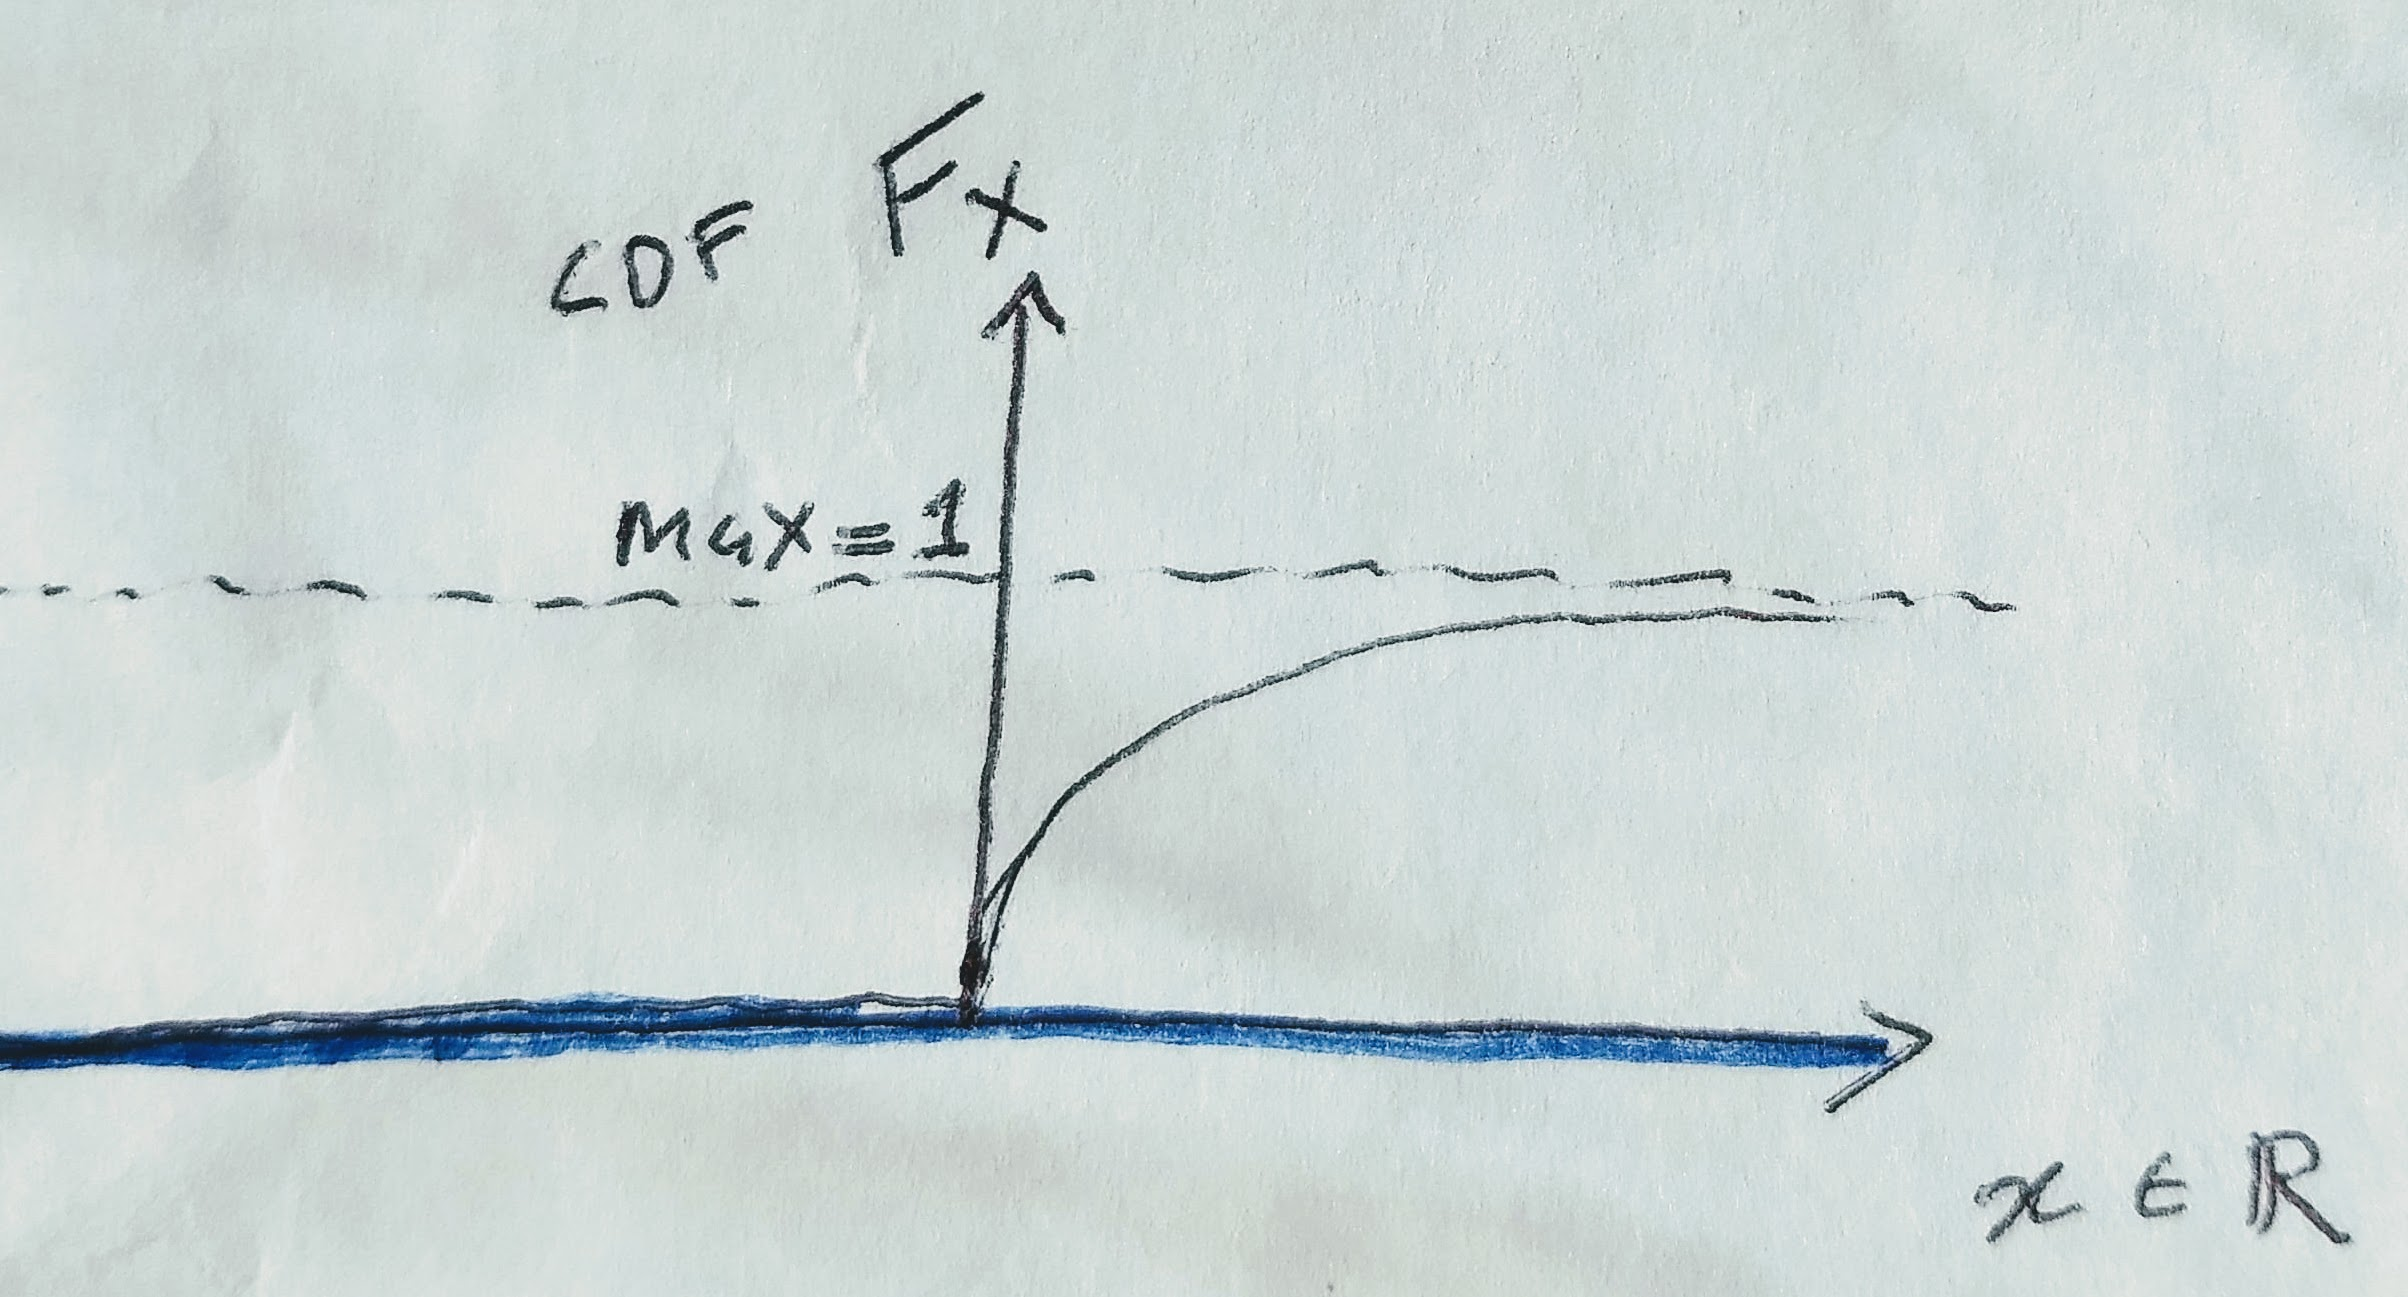
\includegraphics[width=0.4\linewidth]{figures/cdf-exp}
\end{center}

\point{Hint:} use the construction from the ``proof idea'' of Section~\ref{sec:limit-properties-cdfs}, which is called the ``inverse CDF.''


\subsection{$\sigma$-algebra, revisited}\label{sec:sigma-alg-and-estimator}

Often it is useful to put some restrictions on what a random variable can depend on. For example, a model may have two random variables, $Y$ which is observed, and $X$ which is unknown. A statistical estimator $\delta$ should only depend on $Y$, not $X$. 

\point{Method 1: } One way to do this is to force $\delta$ to be a composition based on $Y$ only: $\delta = f(Y)$ for some $f$. 

\point{Method 2: } There is another equivalent way to do that based on the $\sigma$-algebra generated by a random variable, defined as:
\[ \sigma(Y) = \{ (Y \in B) : B \in \borels\}, \]
(Exercise: this is a $\sigma$-algebra). 

\point{Equivalence of the 2 methods: } In an optional question in the assignment, you will show: $\sigma(\delta) \subset \sigma(Y)$ if and only if $\delta = f(Y)$ for some measurable $f$.

\point{Notation:} We use the shorthand $\delta \in \sigma(Y)$ for $\sigma(\delta) \subset \sigma(Y)$.

\point{Exercise:} To get a feeling for what this means, consider $X = (X_1, X_2)$ as the value on two dice, but you only observed their sum $Y$. We want an estimator for $X_1$ based on the observed sum. Consider $\delta_1 = 6 \1[Y > 6] + \1[Y \le 6]$ and $\delta_2 = X_1$. Check $\delta_1 \in \sigma(Y)$ but $\delta_2 \notin \sigma(Y)$.

\point{Answer:} 
\begin{align*}
\Omega &= \{ (i, j) : i,j \in \{1, 2, \dots, 6\} \\
\sigma(X) &= 2^{\Omega} \\
\sigma(Y) &= \sigma(\{\{(1,1)\}, \{(2,1), (1,2)\}, \{(1,3),(2,2),(3,1)\}, \dots, \{(6,6)\}\}) \\
&= \sigma( \{ \{(i,j) : i + j = k\}   : k = 2, 3, \dots, 12  \} ) \\
\sigma(\delta_1) &= \sigma( \{ \{(i,j) : i + j > 6\}, \{(i,j) : i + j \le 6\}  \} ). 
\end{align*}


\subsection{Exercise set 2}\label{sec:ex-set-2}

\begin{enumerate}
  \item Let $X$ be a random variable with a uniform distribution on $[0, 2)$. Draw a possible graph of $X$, a density for $X$, and the \CDF\ of $X$.
  \item Solve the exercise in Section~\ref{sec:generated}.
  \item Solve the exercise in Section~\ref{sec:composition-of-rv}.
  \item Solve the exercise in Section~\ref{sec:density-first-def}.
  \item Solve the exercise in Section~\ref{sec:inverse-cdf}.
  \item If $X_1 \sim F$ (a notation that means that $\P(X_1 \le x) = F(x)$), and $X_1 \ge 0$, find the \CDF\ of $X_2 \defeq X_1^2$.
\end{enumerate}
 

\subsection{Solutions for exercise set 2}

\begin{enumerate}
  \item The three pictures should be as follows:
\begin{center}
	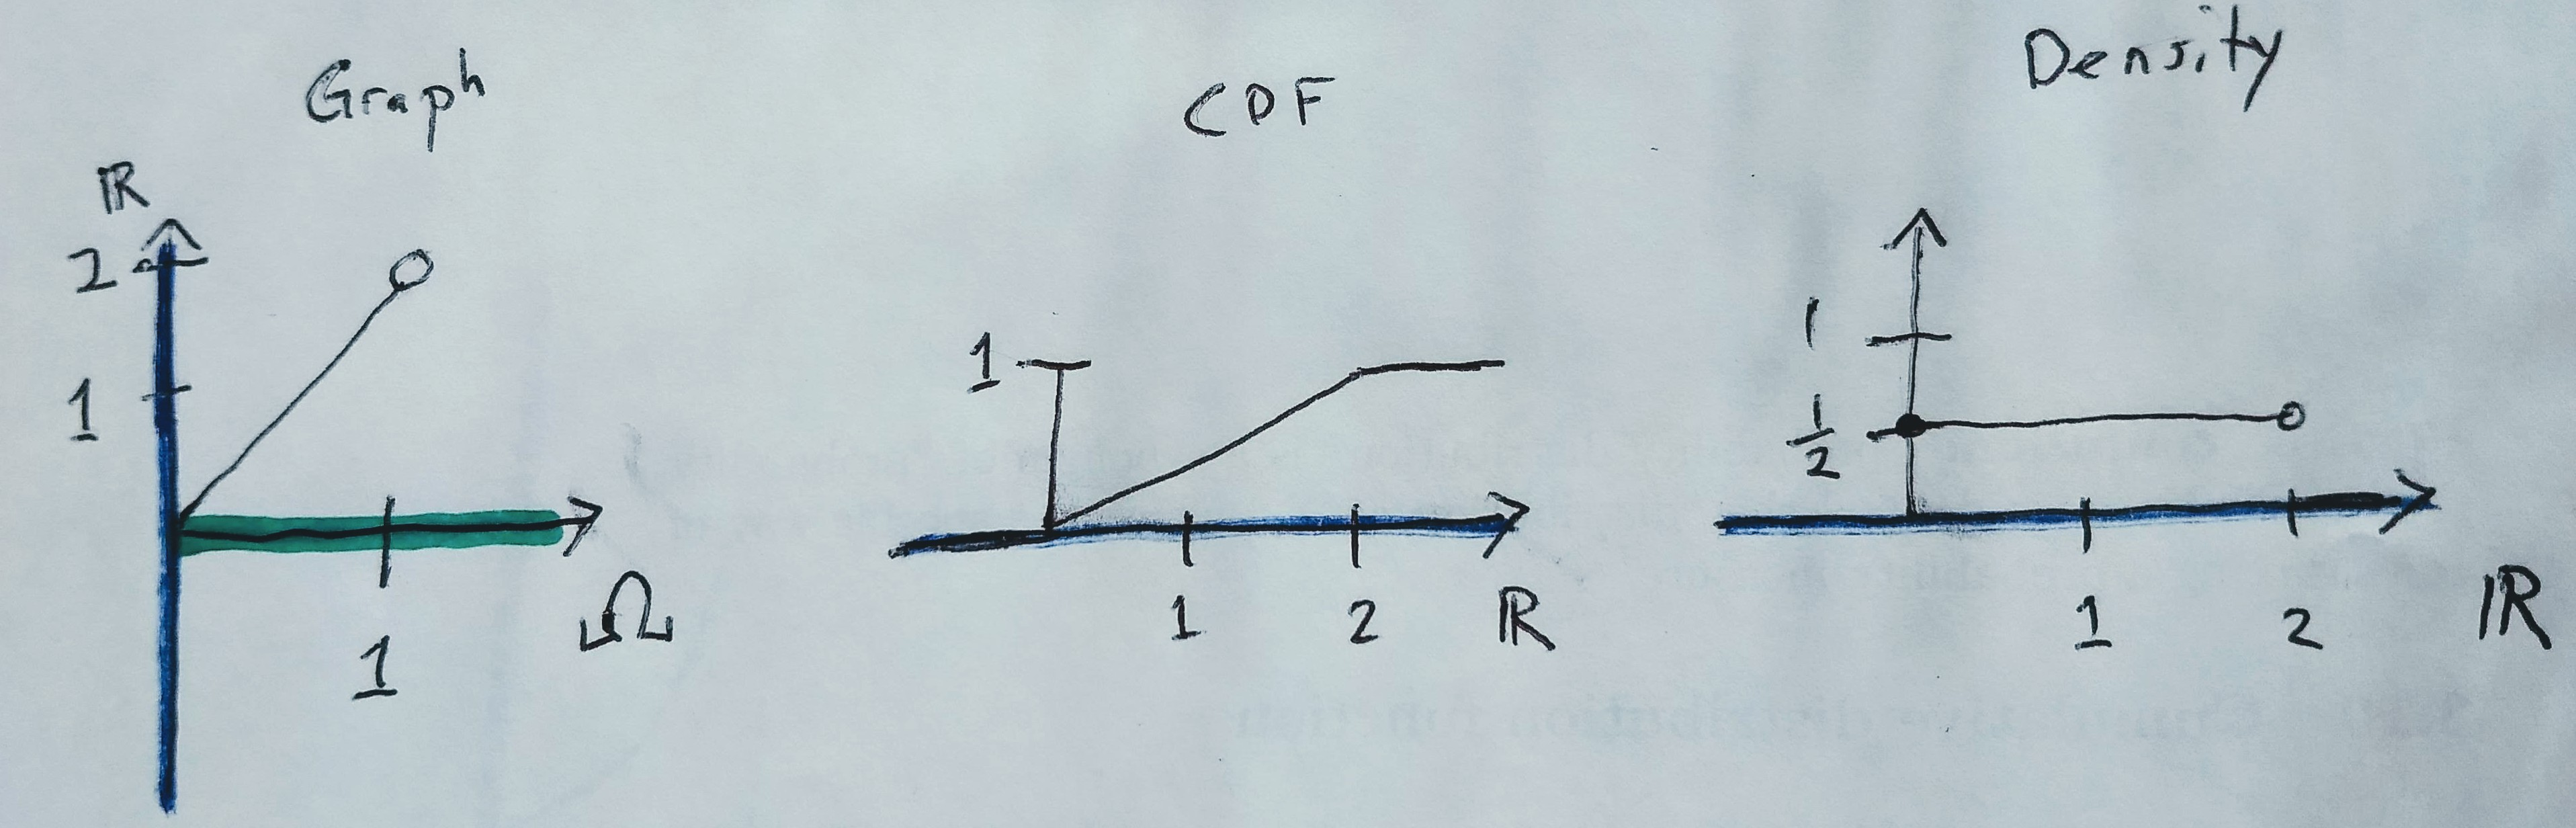
\includegraphics[width=0.9\linewidth]{figures/3-viz}
\end{center}
  \begin{enumerate}
    \item Graph of $X$: The $x$-axis should be a bounded segment labelled $\Omega$. The $y$-axis should be the full real line. There are several choices for the function. For example the line $y = x$ or $y = 1 - x$ on the interval $[0, 1)$ are acceptable. Other choices are possible.
    \item CDF: The $x$-axis should be the full real line. The $y$ axis should be the interval $[0, 1]$. The function should be zero in $(-\infty, 0]$, then affine in $[0, 1]$, then one in $[1, +\infty)$.
    \item Density: the $x$ axis should be the full real line. The $y$ axis should be the positive real line. The function should be the indicator on the set $[0, 1)$.
  \end{enumerate}
  \item We need to check the three conditions given in the definition of \sigmaalg:
  \begin{enumerate}
    \item Since $\events$ is a \sigmaalg, $\Omega \in \events$ and since $\events'$ is a \sigmaalg, $\Omega \in \events'$, therefore $\Omega \in \events \cap \events'$.
    \item We need to show that if $A_1, A_2, \dots$ are all in $\events \cap \events'$, then $\cap A_i \in \events \cap \events'$. By the definition of intersection, we have that $A_1, A_2, \dots$ are all in $\events$. Since $\events$ is a \sigmaalg, it follows that $\cap A_i \in \events$. By the same reasoning, $\cap A_i \in \events'$. Therefore, $\cap A_i \in \events \cap \events'$.
    \item We need to show that if $A \in \events \cap \events'$, then $A^\complement \in \events \cap \events'$. By the definition of intersection, we have that $A \in \events$. Since $\events$ is a \sigmaalg, it follows that $A^\complement \in \events$. By the same reasoning, $A^\complement \in \events'$. Therefore, $A^\complement \in \events \cap \events'$.
  \end{enumerate}
  \item We have that $X: \Omega \to \states$ and $g : \states \to \states'$ are random variables. Let us denote by $\events_\Omega, \events_{\states}$ and $\events_{\states'}$ the \sigmaalg\ on $\Omega$, $\states$ and $\states'$ respectively. Let $A \in \events_{\states'}$. We have to show that $(g \circ X)^{-1}(A) \in \events_\Omega$. First, note that $(g \circ X)^{-1}(A) = X^{-1}(g^{-1}(A))$. Since $g$ is a random variable, $g^{-1}(A) \in \events_\states$. Next, since $X$ is a random variables, $g^{-1}(A) \in \events_\states$ implies that $X^{-1}(g^{-1}(A)) \in \events_\Omega$.
  \item Examples are common. The uniform distribution on $[0, 1/2)$ has height 2.
   \item As in Section~\ref{sec:limit-properties-cdfs}, we pick $X(\omega) \defeq \sup\{x : F(x) < \omega\}$ (note that in this special case were $\Omega = [0, 1)$,  writing ``$F(x) < \omega$'' is well defined---for general $\Omega$ is would not).
	This construction has some nice properties (draw a picture of a \CDF\ having flat regions as well as discontinuities to convince yourself, as these are the interesting ``corner cases''):
	\begin{enumerate}
	  \item \label{point:inv-cdf-monotone} $X$ is monotone increasing,
	  \item \label{point:inv-cdf-incl-one} $X\circ F(x) \le x$,
	  \item \label{point:inv-cdf-incl-two}$F\circ X(\omega) \ge \omega$.
	\end{enumerate}
	We first use properties \ref{point:inv-cdf-incl-one} and \ref{point:inv-cdf-incl-two} to prove the following set equality:
	\[ (X \le x) = \{\omega \in \Omega : \omega \le F(x) \}.\]
	We show that the LHS includes the RHS and vice versa:
	\begin{itemize}
	  \item $\{\omega \in \Omega : \omega \le F(x) \} \subseteq (X \le x)$:
	\begin{eqnarray*}
	\omega \le F(x) &\Longrightarrow& X(\omega)  \le X\circ F(x)\;\text{ (from \ref{point:inv-cdf-monotone})} \\
	&\Longrightarrow& X(\omega) \le x\;\text{(from \ref{point:inv-cdf-incl-one}).}
	\end{eqnarray*}
	  \item $(X \le x) \subseteq \{\omega \in \Omega : \omega \le F(x) \}$:
	\begin{eqnarray*}
	X(\omega) \le x &\Longrightarrow& F\circ X(\omega)  \le F(x)\;\text{ (monotonicity of CDFs)} \\
	&\Longrightarrow& \omega \le F(x)\;\text{(from \ref{point:inv-cdf-incl-two}).}
	\end{eqnarray*}
	\end{itemize}
	Finally, it follows that:
	\begin{eqnarray*}
	\text{CDF of }X &\defeq& \P(X \le x) \\
	&=& \P\{\omega \in \Omega : \omega \le F(x) \} \\
	&=& F(x) \;\text{ (by the definition of uniform probability).}
	\end{eqnarray*}
	Here in this special case: $X(\omega) = - \lambda^{-1} \log(1 - \omega)$.
	\item We have:
	\begin{eqnarray*}
	F_{X_2}(x) &\defeq& \P(X_2 \le x) \\
	&=& \P(X_1^2 \le x) \\
	&=& \P(-\sqrt{x} \le X_1 \le \sqrt{x}) \\
	&=& \P(X_1 \le \sqrt{x}) \;\text{(Non-negativity assumption)} \\
	&=& F(\sqrt{x}).
	\end{eqnarray*}
\end{enumerate}


\section{Integration and expectation} 

\subsection{Overview}

\point{How to define the mean?} At an undergraduate level, this is usually done as follows for continuous random variables:
\[ \E[X] \defeq \int_{-\infty}^{+\infty} x f(x) \ud x, \]
where $f$ is the density of $X$. There are two limitations with this definition:
\begin{enumerate}
  \item it is not very intuitive (why multiply the density with an $x$?),
  \item we need a separate definition for discrete random variable (and what about cases where we have both continuous and discrete parts?).
\end{enumerate}

\point{Better definition:} the expectation is the area under the graph of $X$!

\point{Note:} we will need to generalize the notion of ``area,'' to cover cases where $\Omega \neq \R$.

\point{Terminology:} the definition of integral we will cover today is called the Lebesgue integral (not to be confused with the Lebesgue measure). It is the default definition in measure theory, and in general in probability theory.

\point{Note:} we will get the undergraduate definition of expectation of a continuous random variable as a special case arising when $X$ has a density. However, the Lebesgue expectation does not need to assume existence of a density.


\subsection{Notation, inputs and outputs}

The integral you know from calculus (called the Riemann integral) takes one input (a function $f : \R \to \R$) and return one real number. In contrast, the Lebesgue integral needs \emph{two} inputs:
\begin{enumerate}
  \item a probability measure $\P : \events \to [0, 1]$, where $\events$ is a \sigmaalg\ on a sample space $\Omega$,
  \item a random variable $X : \Omega \to \R$.
\end{enumerate}

\point{Notations from real analysis:} you will see different notations depending on the author/community to encode this operator on two inputs, for example (these are all synonyms):
\begin{itemize}
  \item $\int X \ud \P$
  \item $\int X(\omega) \P(\ud \omega)$
  \item $\P X$
  \item $(\P, X)$.
\end{itemize}

In probability theory and Bayesian statistics, there is often a ``global'' probability $\P$. When this is the case:

\point{Notation in probability theory/Bayesian statistics:} 
\[ \E[X] \defeq \int X \ud \P. \]



\point{Frequentist statistics:} in this branch of statistics, there is often a collection of probabilities indexed by a parameter $\theta$, i.e. $\{\P_\theta : \theta \in \Theta\}$. When this is the case:
\[ \E_\theta[X] \defeq \int X \ud \P_\theta. \]


\subsection{Generalizing the notion of the ``area'' of a ``rectangle''}

Let us start by defining the notion of area under the curve for something simple: an indicator function multiplied by a constant, $Z = a \1_A$. To make it easier to visualize, let us make this assumption from now on (we will relax it at some point later):

\point{Assumption:} assume that all random variables take values $\ge 0$.

Now if $A$ is an interval, the graph is just a rectangle! The height is $a$. What should be the base? Since we are given a probability, let us use it to measure the base, giving $\P(A)$ for the base. This suggests:

\point{Definition:} the Lebesgue integral for indicator function is given by 
\[ \E[Z] = \int Z \ud \P \defeq a \P(A). \]
\begin{center}
	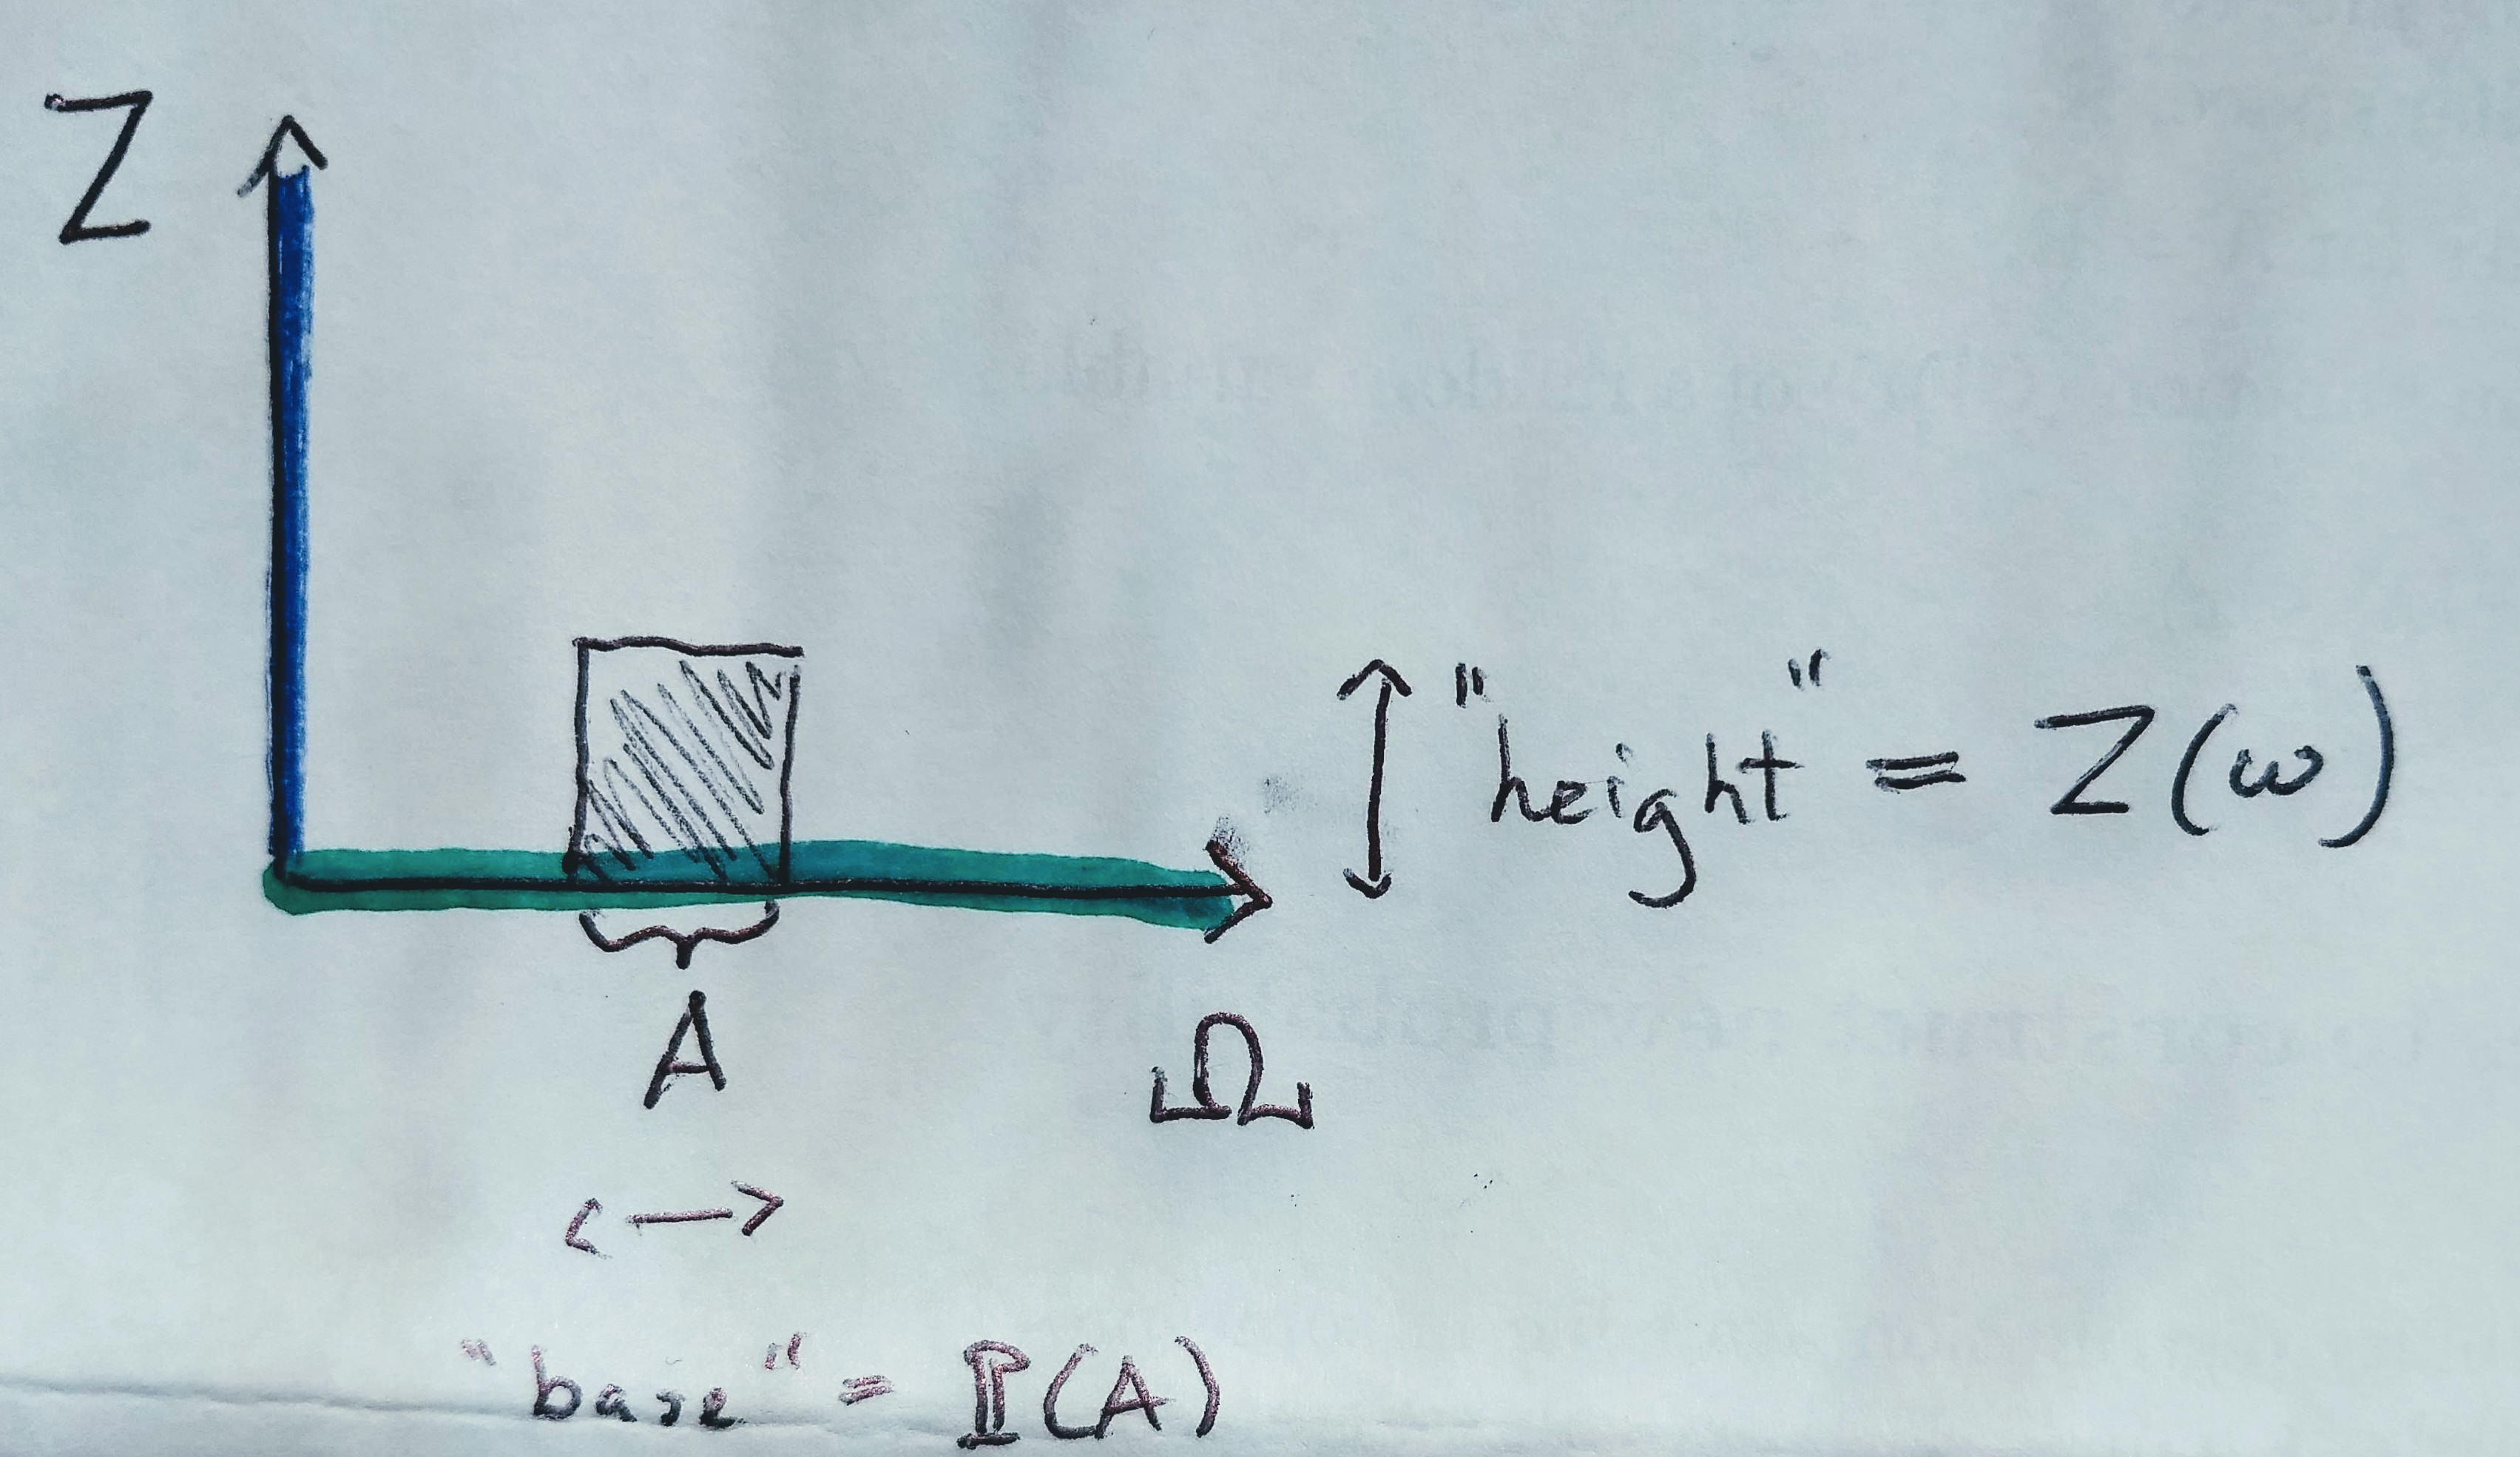
\includegraphics[width=0.5\linewidth]{figures/rectangle}
\end{center}

\point{Note:} $A$ could actually be complicated (e.g., the Cantor set), but this definition still holds as long as $A \in \events$.

\point{Note:} there will be cases (especially when we talk about limits) where the base has measure zero, but the height is infinite. We would like our definition to return zero in these cases (since the function blows up on a negligeable set). For this reason, we define $0 \times \infty = 0$.

\point{Exercise:} compute the expectation of a constant.

\point{Important special case:} following from the definition directly, the expectation of an indicator on an event $A$ is just the probability of $A$, i.e. \[\E[\1_A] = \P(A).\] In light of the answer of the exercise in Section~\ref{sec:distribution}, we only need the distribution of the indicator random variable to compute its expectation. As we will see soon, this is always true, i.e. we only need the distribution of a random variable in order to compute its expectation. In other words, all random variables sharing the same distribution have the same expectation (and many distinct random variables do share the same distribution, see Section~\ref{sec:equal-in-distribution}). 

\point{Exercise:} based on the above special case, can you guess the general formula for computing the expectation of a random variable given only the distribution of the random variable, not the random variable itself?


\subsection{Area under the graph of ``simple functions''}\label{sec:area-simple-function}

\point{Simple function:} a simple function is a random variable of the form
\[ Y = \sum_{i = 1}^N a_i \1_{A_i}, \]
where the $A_i$ are assumed to be disjoint.

\point{Definition:} motivated by linearity we extend the definition of the Lebesgue integral to simple functions:
\[ \E[Y] = \int Y \ud \P \defeq \sum_{i=1}^N a_i \P(A_i). \]

\point{Note:} our previous definition for indicators is just a special case of this, so we are not contradicting ourselves.

\point{Property:} the above definition is motivated by linearity, and important property we want expectations to enjoy:
\[ \E[Y + Y'] = \E[Y] + \E[Y']. \]

\point{Exercise:} prove this property holds for the above definition of integral of simple functions.


\subsection{Area under graph of non-negative random variables}\label{sec:area-non-neg}

Now, how to define the area under the graph of an arbitrary non-negative random variable? We make use of our previous definition for simple functions:

\point{Definition:} let $X \ge 0$ (meaning $X(\omega) \ge 0$ for all $\omega \in \Omega$), 
\[ \E[X] = \int X \ud \P \defeq \sup\left\{ \int Y \ud \P : Y\text{ is simple and } 0 \le Y \le X\right\}. \] 

\point{Exercises:} show $\E[X] \ge 0$ and monotonicity: $X \le Y \Longrightarrow \E[X] \le \E[Y]$. 


\subsection{Algorithmic construction}

To avoid having to deal with an uncountable collection we follow a two steps strategy:
\begin{enumerate}
  \item express the random variable to integrate $X$ as the limit of a sequence of increasing and simple random variables. This is done using: \\\point{Proposition:} (approximation by simple functions) For any random variable $X \ge 0$, there exists a sequence of random variables $0 \le Y_1 \le Y_2 \le \dots$ such that:
   \begin{enumerate}
     \item each $Y_n$ is simple, and
     \item for all $\omega \in \Omega$, $\lim_{n\to\infty} Y_n(\omega) = X(\omega)$ (this property is known as \point{pointwise convergence}, denoted $Y_n \to X$, or in this case since the r.v. are additionally increasing, $Y_n \uparrow X$).
   \end{enumerate}
  \item We will use the \point{monotone convergence theorem (MCT)} to exchange the limit and integral: if $0 \le Y_1 \le Y_2 \le \dots$ are non-negative random variables (not necessarily simple, although they are in this specific context), then 
\[ \underbrace{ \int (\lim_{n\to\infty} Y_n) \ud \P}_{\text{hard!}} = \lim_{n\to\infty} \underbrace{\int Y_n \ud \P.}_{\text{easier!}} \]
\end{enumerate}

\point{Proof idea} of the proposition on approximation by simple functions: 
\begin{enumerate}
  \item Recall that in the case of a Riemann integral, we do something similar, i.e. breaking the x-axis of the graph of $X$ into a grid and making this grid finer and finer.
  \begin{center}
  	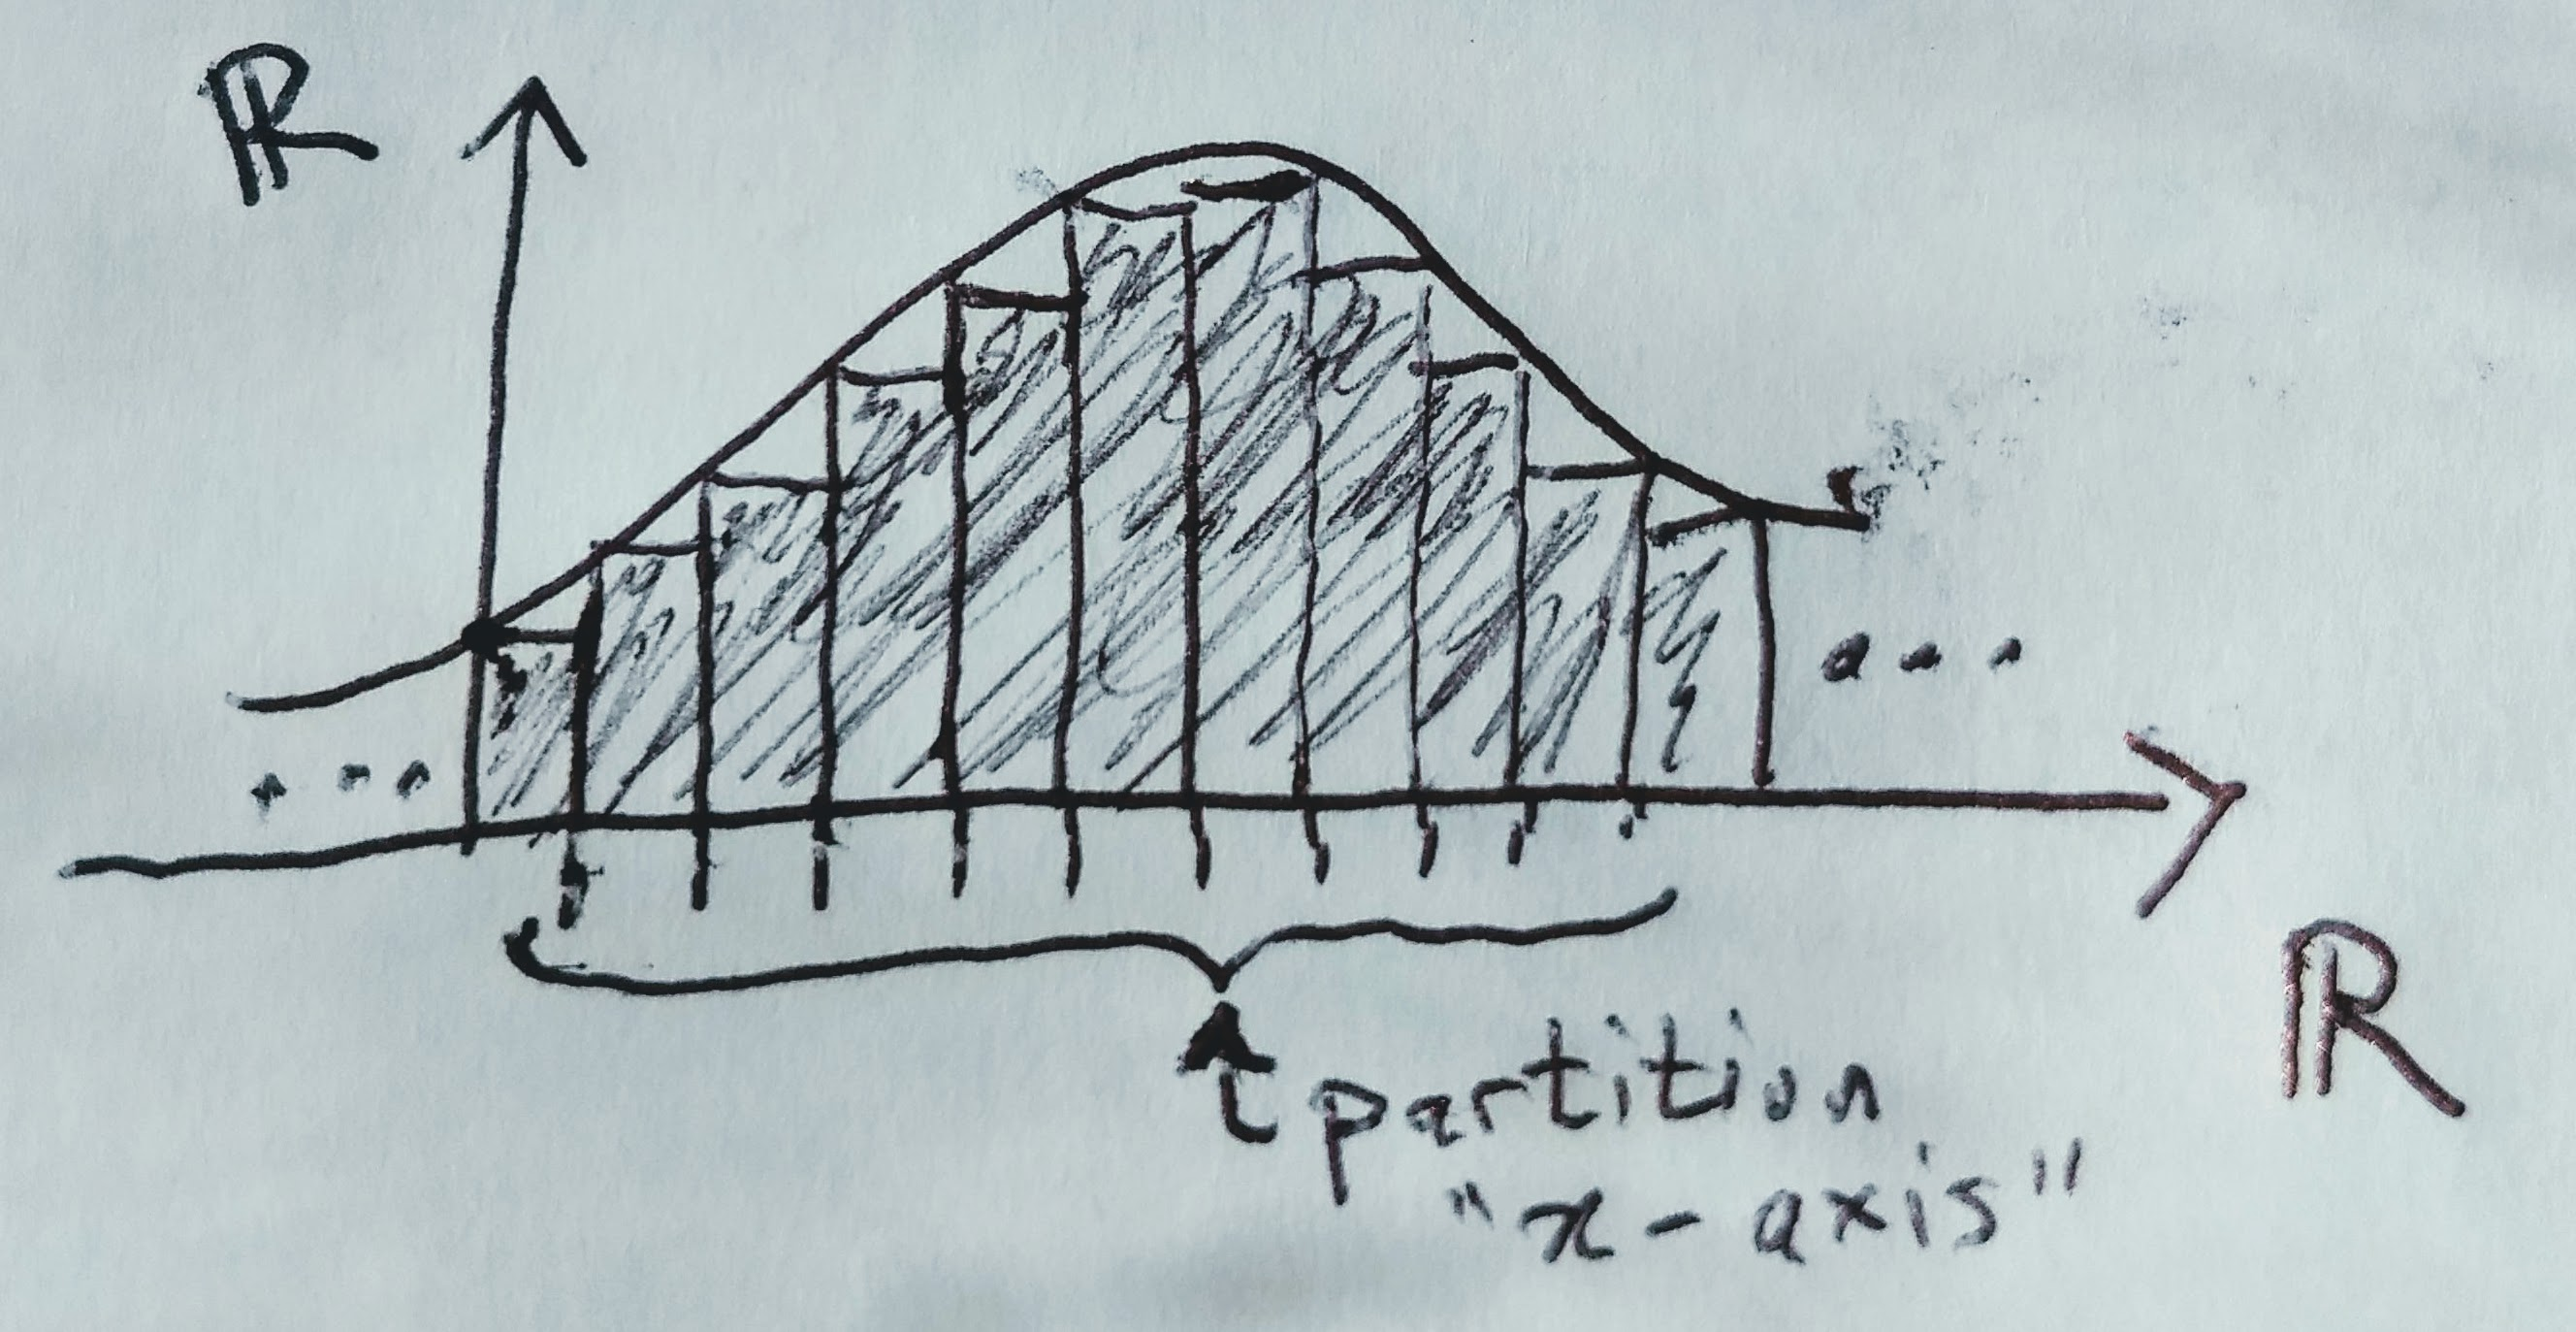
\includegraphics[width=0.5\linewidth]{figures/riemann}
  \end{center}
  \item In general, this cannot work here, because the x-axis, $\Omega$, is not necessarily $\R$. 
  \item Idea: break the $y$-axis instead! Then use the inverse of the random variable $X^{-1}$, to get the $A_i$'s required in the definition of simple functions.
  \begin{center}
  	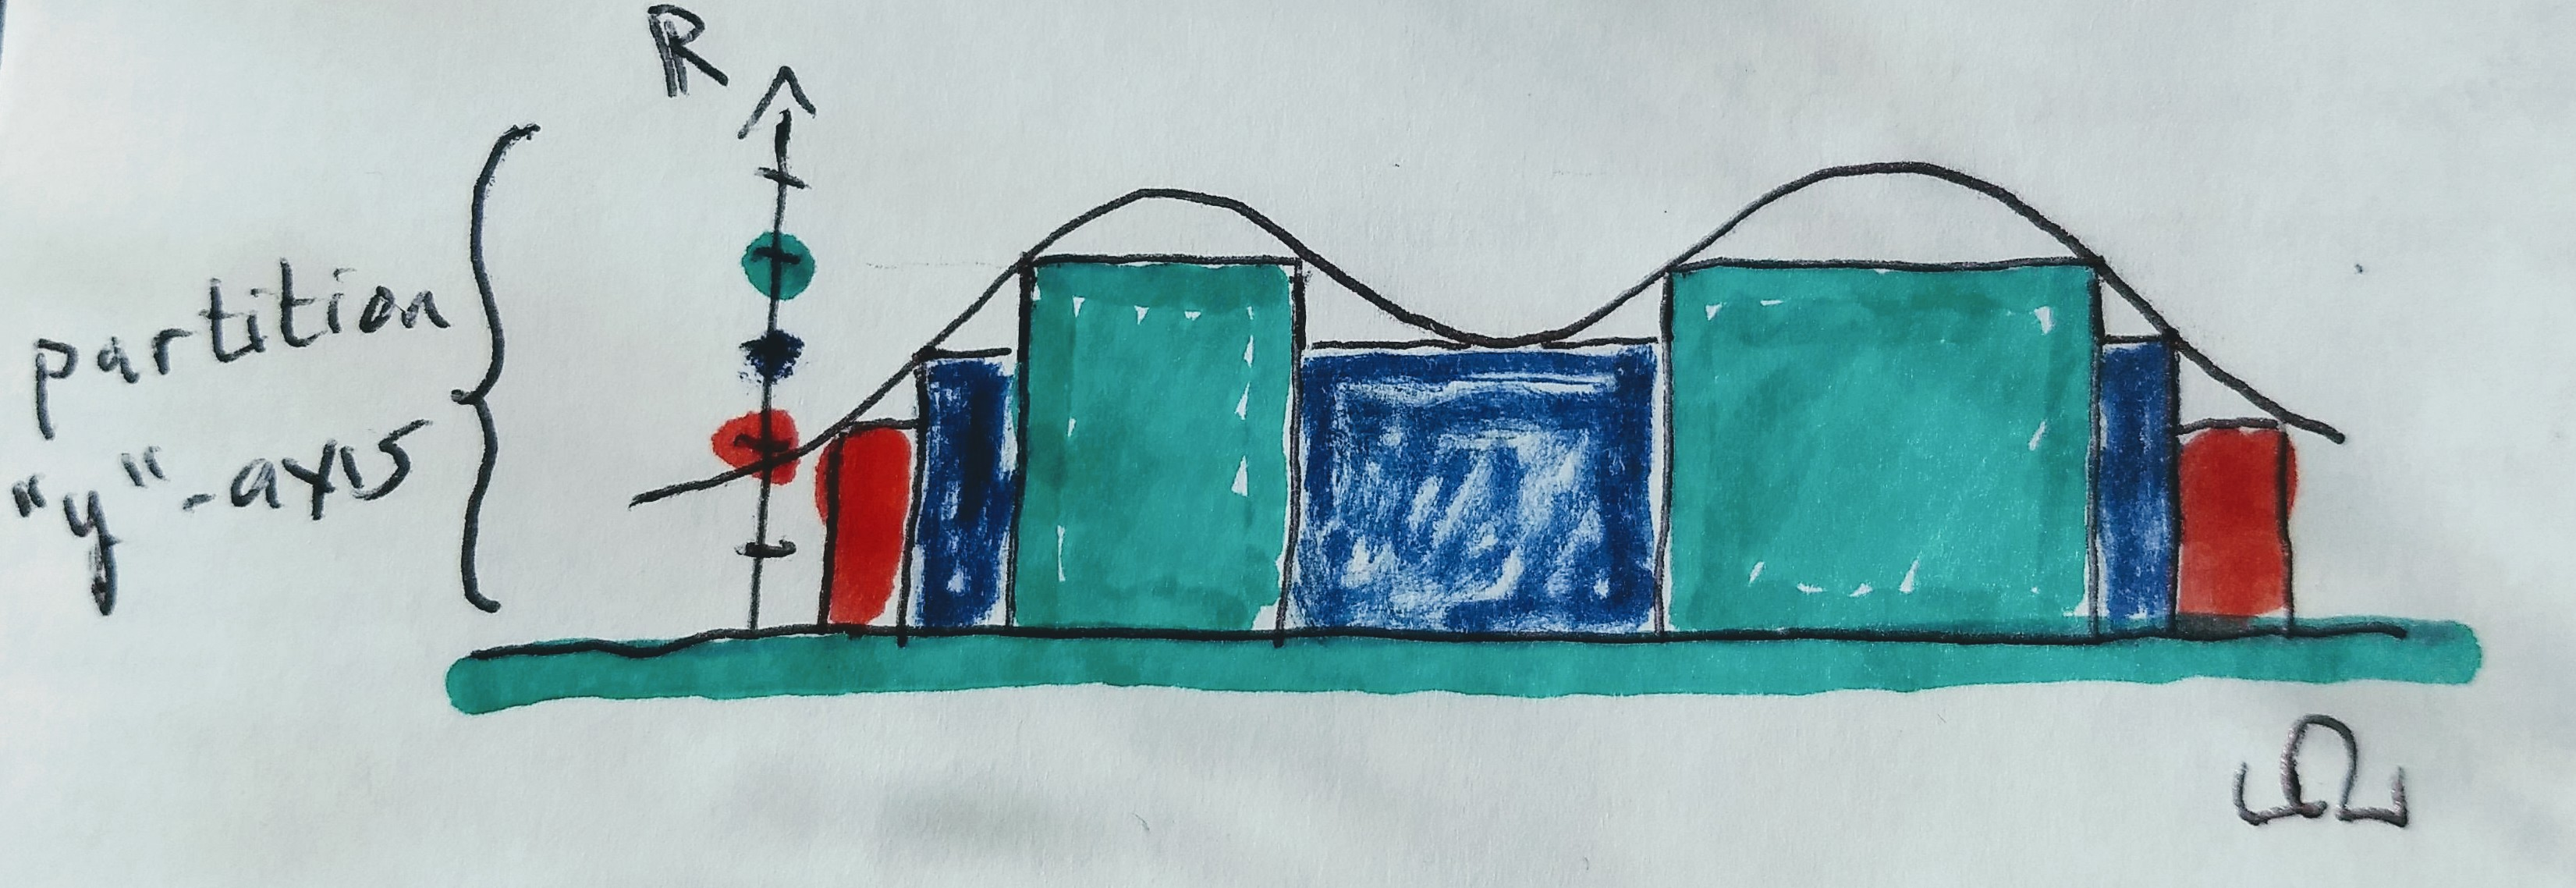
\includegraphics[width=0.7\linewidth]{figures/lebesgue}
  \end{center}
\end{enumerate}


\subsection{Proving tool: simple function approximation +  MCT}\label{sec:approxAndMCT}

The previous section sets the stage for a powerful proving strategy:
\begin{enumerate}
  \item Suppose you want to prove an identity involving expectations.\\\point{Example:} linearity for non-negative random variables $X, X' \ge 0$, \[ \E[X + X'] = \E[X] + \E[X']. \]
  \item First prove that the identity holds for simple random variables \\\point{Example:} that was an earlier exercise in the case of linearity.
  \item Then, use the approximation theorem to get simple $Y_n \uparrow X$ and $Y'_n \uparrow X'$. 
  \item Use MCT to conclude. \\\point{Example:}
\begin{eqnarray*}
\E[X + X'] &=& \E[ \lim (Y_n + Y'_n) ] \\
&=& \lim \E [Y_n + Y'_n] \;\;\;\text{ (we can use MCT here since }0 \le Y_n + Y'_n \uparrow X + X'\text{)} \\
&=& \lim ( \E[Y_n] + \E[Y'_n] ) \;\;\;\text{ (easy to prove since }Y_n, Y'_n\text{ are simple)} \\
&=& \lim \E[Y_n] + \lim \E[Y'_n] \;\;\;\text{ (properties of limits of real sequences)} \\
&=& \E[X] + \E[X'] \;\;\;\text{ (MCT again, twice).}
\end{eqnarray*}
\end{enumerate}

\point{Easy extension:} $\E$ is a linear operator: $\E[aX + b] = a\E[X] + b$.

\point{Note:} this proving strategy is incredibly useful in practice, in part thanks to how simple the statement of the monotone convergence theorem is. Similar statements with Riemann integrals are not as simple. Just this proving method arguably justifies the effort of learning to be a user of measure theory. 


\subsection{Integrals of random variables taking negative values}

For a general random variable $X$:
\begin{center}
	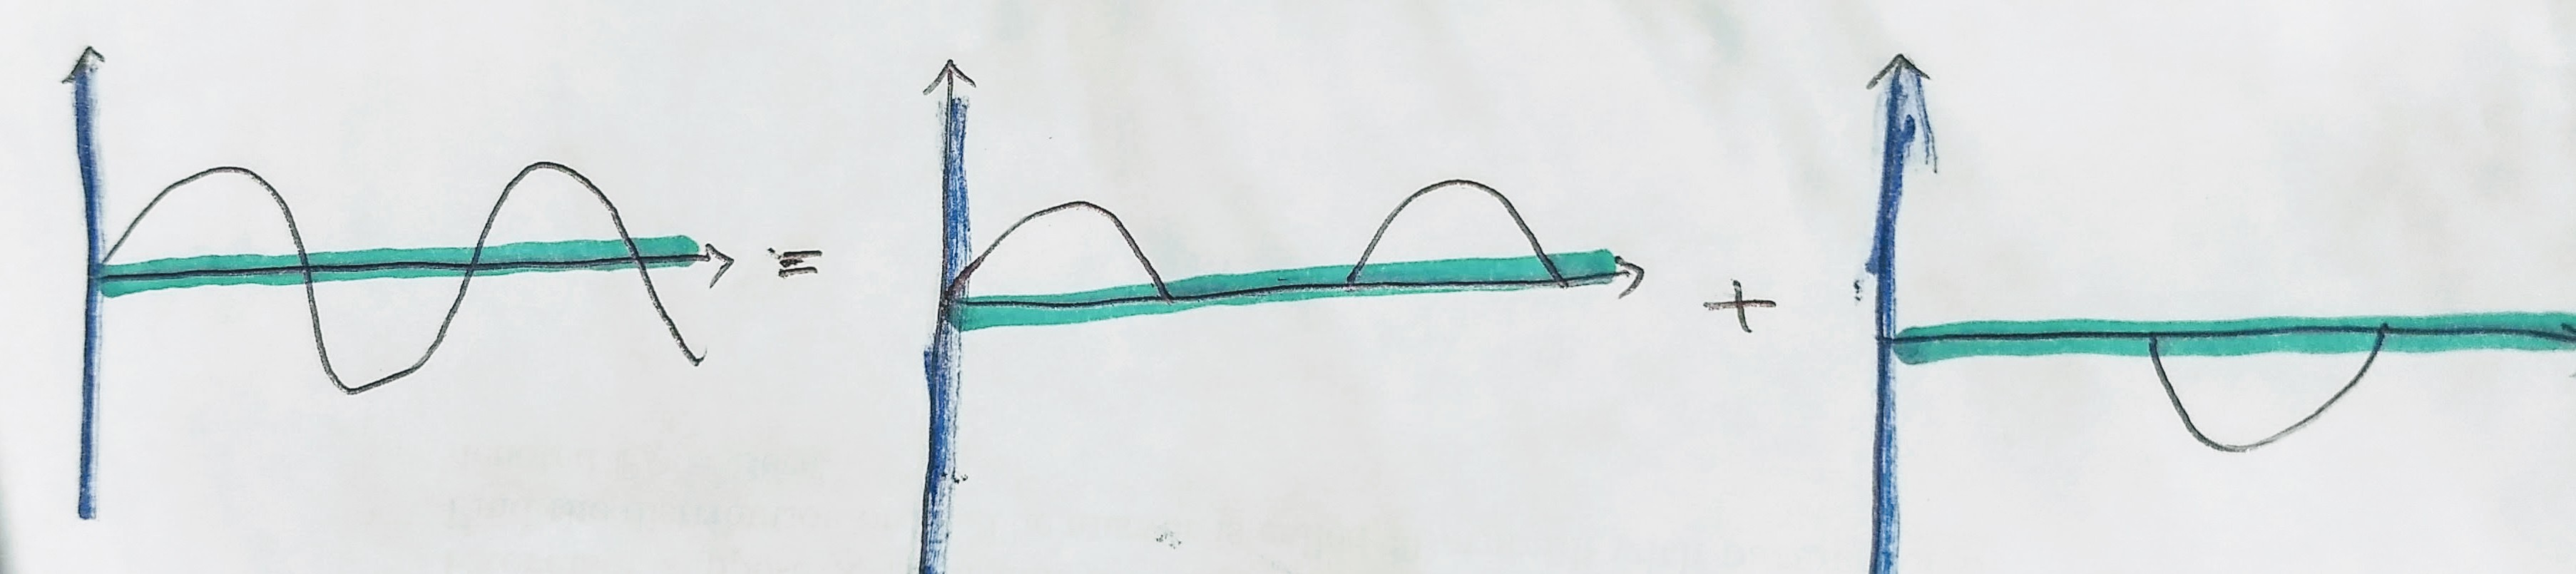
\includegraphics[width=0.8\linewidth]{figures/decomposition}
\end{center} 
\begin{enumerate}
  \item Write $X = X^{+} + X^{-}$, where $X^{+}$ and $X^{-}$ are the negative and positive parts respectively. For example, $X^{-} = \1[X < 0] X$. 
  \item Note: $-X^{-}$ is non-negative.
  \item Compute $I^{+} \defeq \E[X^+]$ and $I^{-} \defeq \E[-X^-]$.
  \item If both $I^{+} = I^- = \infty$, return an error (``the Lebesgue integral is not defined''),
  \item else define $\E[X] \defeq I^{+} - I^{-}$.
\end{enumerate}

\point{Terminology:} 
\begin{itemize} 
  \item If at least one of $I^{+}$ and $I^-$ is finite, we say the Lebesgue integral of $X$ is defined,
  \item when both $I^{+}$ and $I^-$ are finite, we say $X$ is \emph{integrable}, denoted $X \in \L_1$. 
\end{itemize}

\point{Exercise:} find a random variable $X \notin \L_1$ such that $\E X$ exists. Find a random variable $Y$ where $\E Y$ is not defined. 


\subsection{Integrals with respect to a measure}

So far, we have assumed that the Lebesgue integral was computed with respect to probability measure $\P : \events \to [0, 1]$. 

\point{Exercise:} go over the above argument again with a measure $\mu : \events \to [0, \infty)$ instead of a probability measure $\P$ and check that everything goes through.



\subsection{More on exchanging limits and integrals}\label{sec:exchange-lim}

The monotone convergence theorem (Section~\ref{sec:approxAndMCT}) says that we can exchange integrals and limits \emph{when the sequence of function is increasing} ($X_1 \le X_2 \le \dots$). Is this necessary?

\point{Example showing that it is:} consider $X_n = n \1_{(0, 1/n]}$. 
\begin{center}
	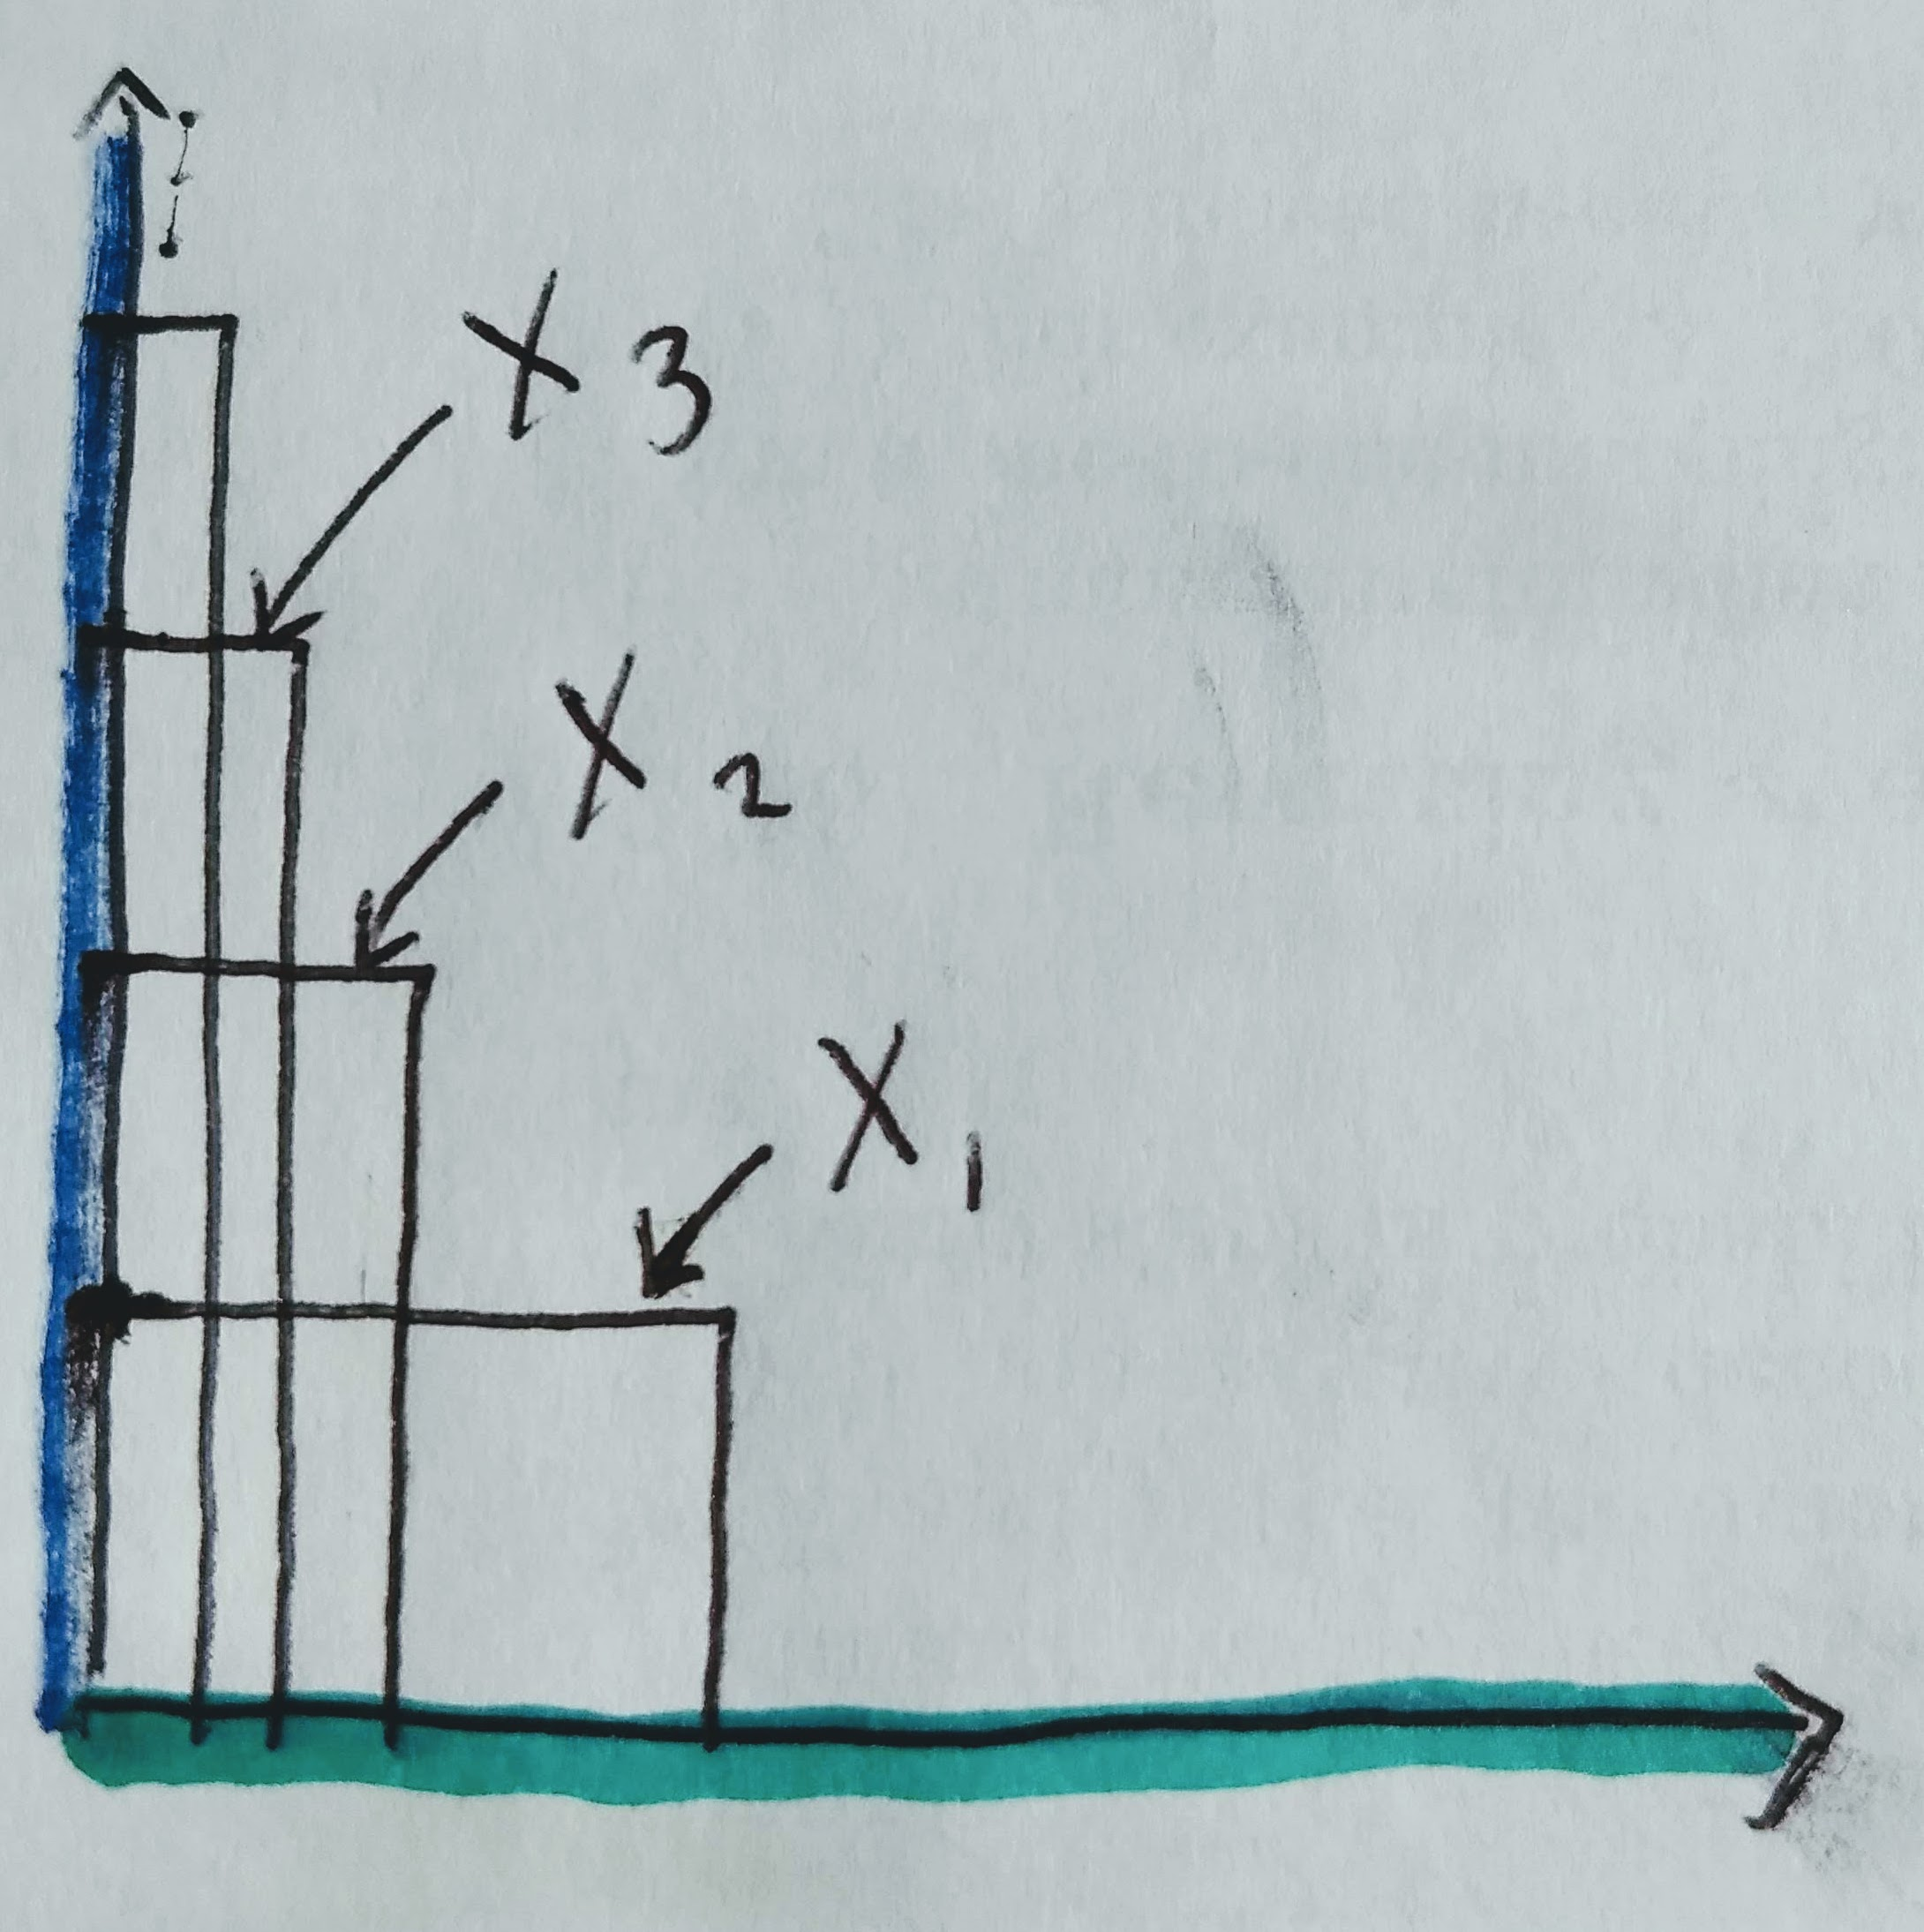
\includegraphics[width=0.4\linewidth]{figures/limit-exchange-warn}
\end{center}

\point{Exercise:} compute $\lim X_n$ and $\E X_n$. Conclude that limits and integrals cannot be exchanged in this case.

\point{However:} there are non-monotone cases where you can exchange limits and integrals. For example, when they have \point{an integrable envelope}, defined as a random variable such that:
\begin{enumerate}
  \item $|X_i| \le Y$,
  \item $\E|Y| < \infty$.
\end{enumerate}

\point{Theorem:} (Dominated Convergence Theorem, DCT) if $X_1, X_2, \dots$ have an integrable envelope, and $\lim X_i$ exists, then $\lim \E X_i = \E \lim X_i$.


\subsection{Measure zero sets and almost sure statements}

As a direct consequence of the axioms of probability, an empty event has probability zero: $\P(\emptyset) = 0$. The converse is not true though. For example under the uniform probability an event that contains only a single point still has probability zero $\P(\{0.2\}) = 0$. In fact, under the uniform probability, events containing countably many points have probability zero.\footnote{Even more surprising, there are set containing uncountably many points that still have probability zero. Read about the Cantor set if you are curious.} 

For this reason, it is often possible to relax a statement like ``$|X_i| \le Y$'' in the previous statement to a statement like ``$|X_i| \le Y$ except for a set of probability zero.'' This second statement is formalized as $\P(|X_i| \le Y \text{ for all }i) = 1$, and denoted ``$|X_i| \le Y$ a.s.''


\subsection{Convexity and integration}\label{sec:convexity}

\point{Review:} convexity. A function $g : \R \to \R$ is convex if for all $x_1, x_2 \in \R$ and $\lambda \in [0, 1]$, 
\[ \lambda g(x_1) + (1 - \lambda) g(x_2) \ge g(\lambda x_1 + (1 - \lambda) x_2). \]
\begin{center}
	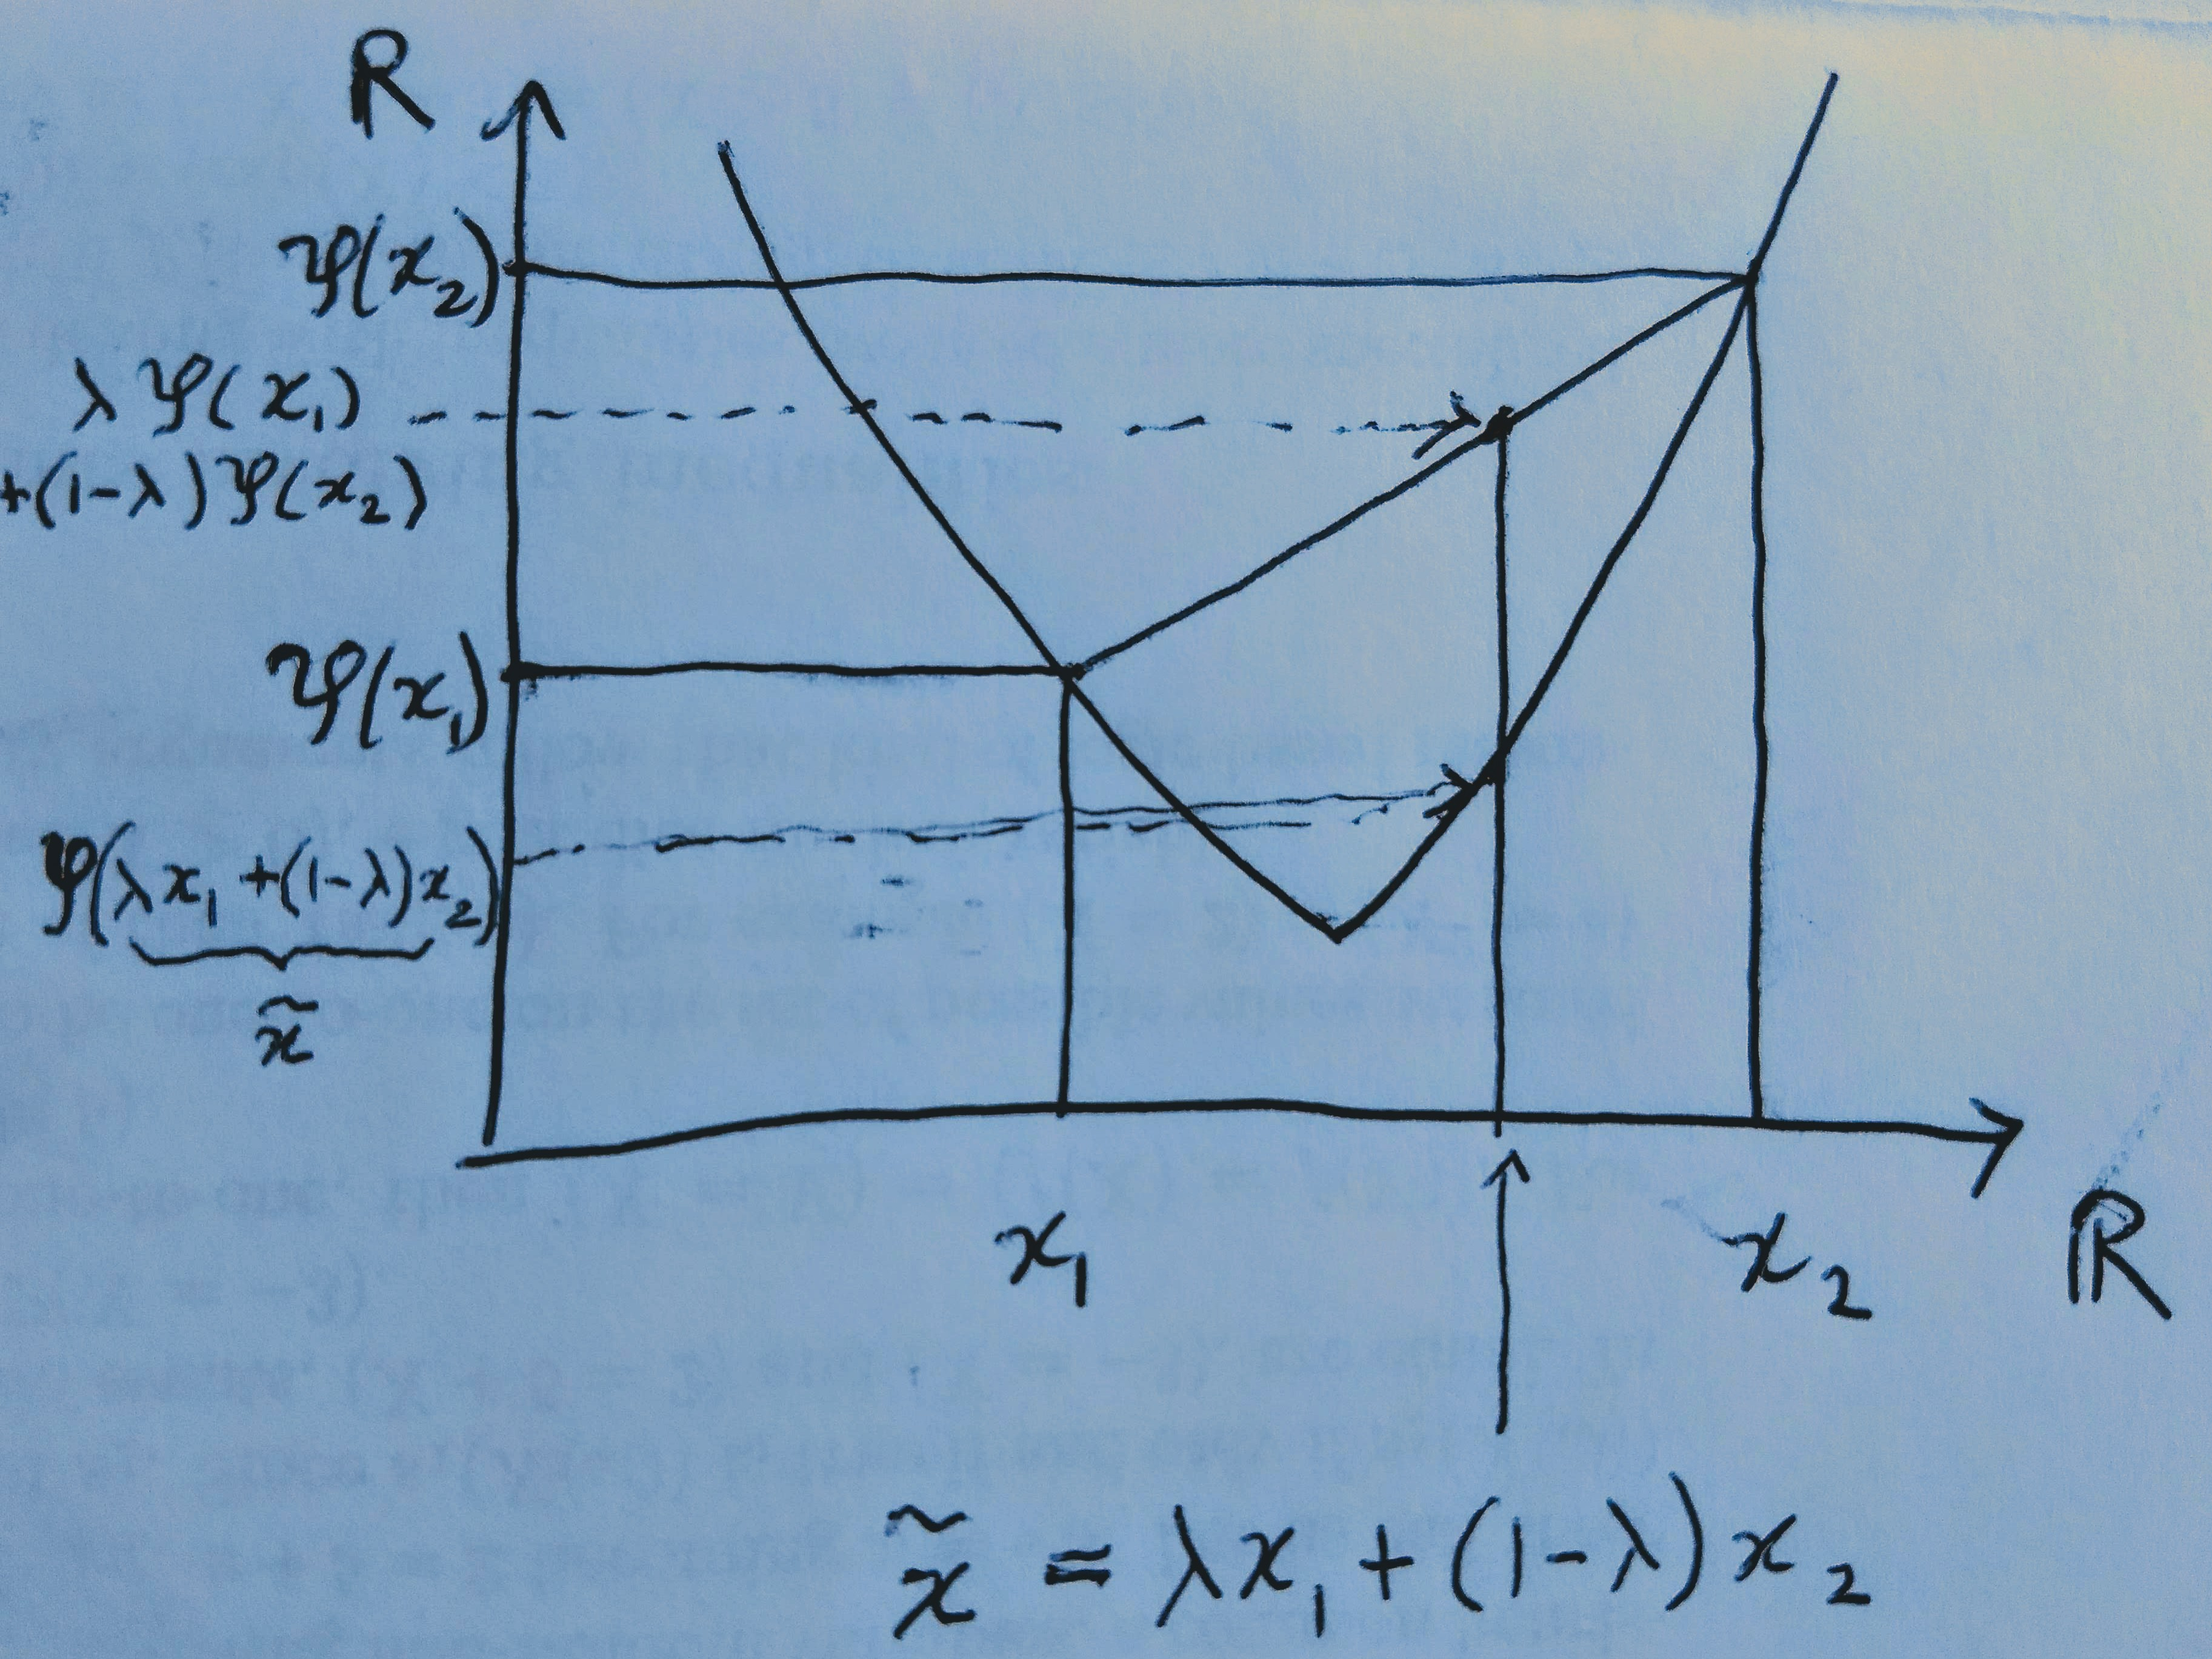
\includegraphics[width=0.6\linewidth]{figures/convex}
\end{center}

\point{Exercise:} convince yourself that $\varphi(\E X) \neq \E[\varphi(X)]$ in general (with some exceptions to this, e.g. when $\varphi$ is linear). This is unfortunate because $\varphi(\E X)$ is often easier to compute than $\E(\varphi(X))$.

\point{However:} if $\varphi$ is convex, we can at least get the following bound.

\point{Jensen's inequality:} if $\varphi$ is convex, then $\varphi(\E X) \le \E[\varphi(X)]$.

\point{Proof:} to prove Jensen's inequality, we will use the following result from convex analysis:

\point{Lemma:} for all convex function $\varphi$, there is a sequence of linear functions $L_n(x) = a_n x + b_n$ such that 
\[ \varphi(x) = \sup_n L_n(x). \]
\begin{center}
	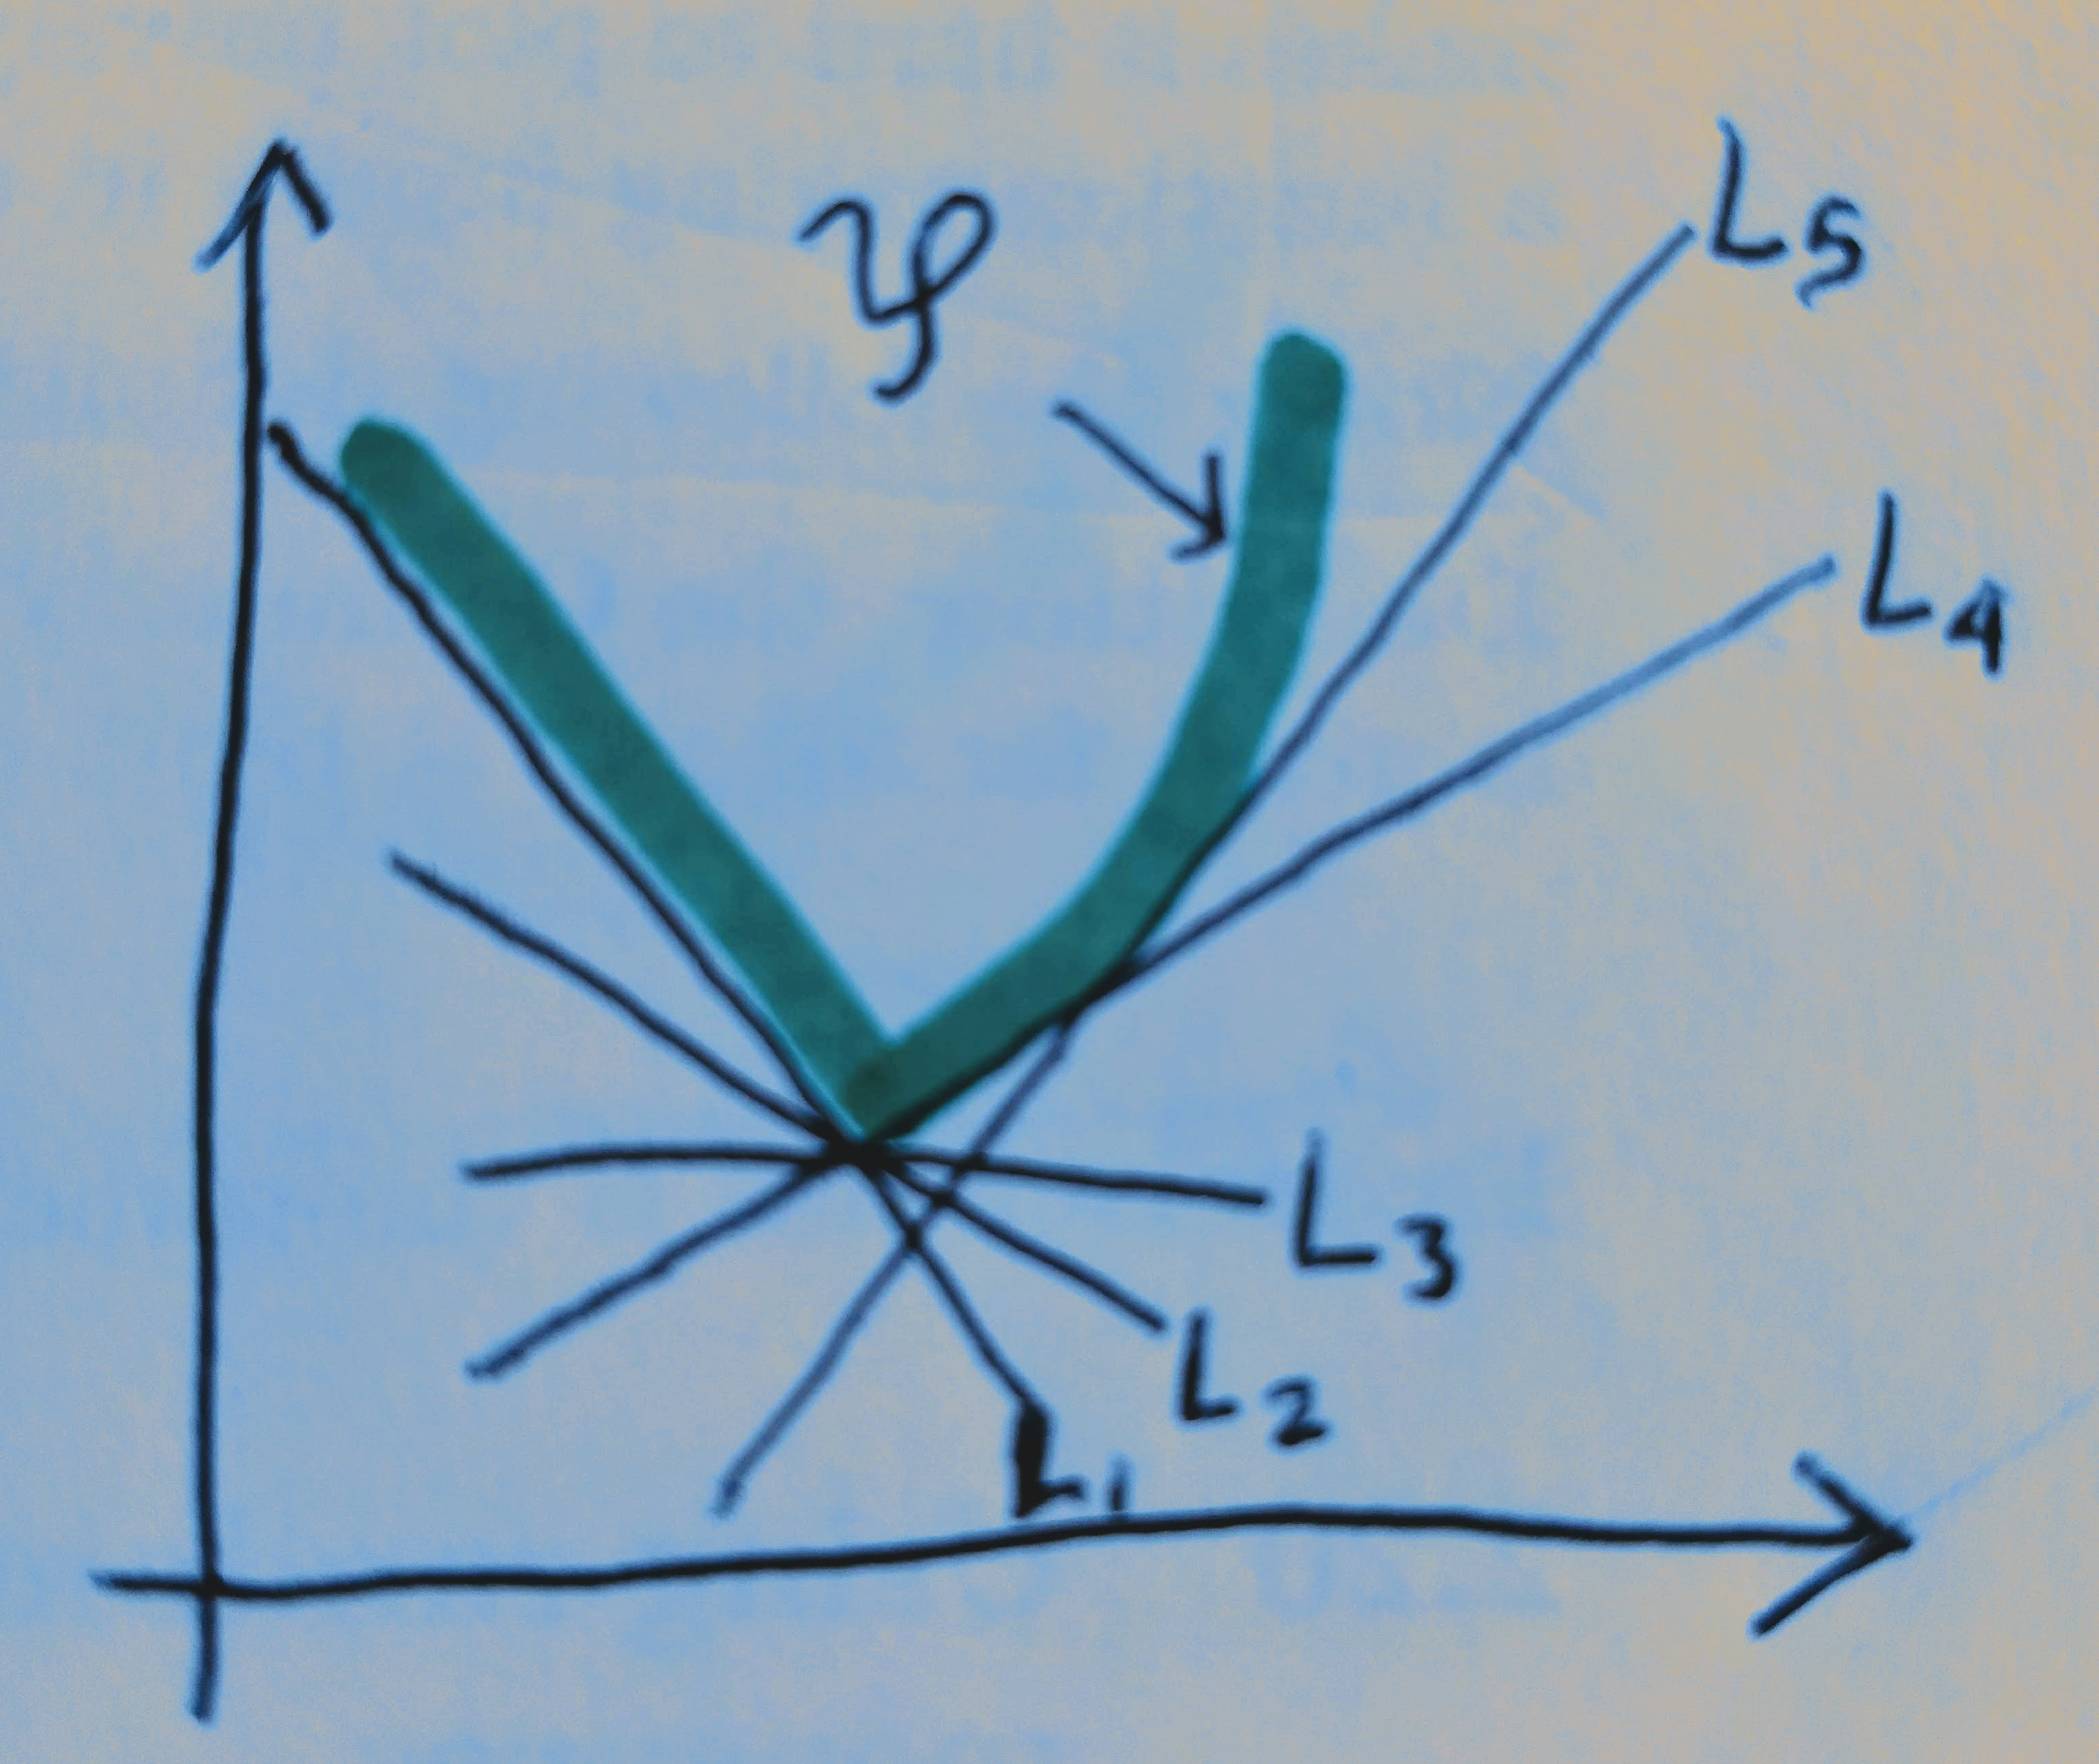
\includegraphics[width=0.3\linewidth]{figures/convex-support}
\end{center}

\point{Exercise:} provide an example showing that the above lemma does not hold in the case for non-convex functions.

\point{Back to Jensen's:} using our lemma, we have $\varphi(X) \ge L_n(X)$ by construction. ``Taking expectations on both sides'' (i.e. using monotonicity of expectations):
\begin{eqnarray}
\E\varphi(X) &\ge& \E[L_n(X)] \\
&=& L_n(\E X) \;\text{ since }L_n\text{ is linear.}
\end{eqnarray}
Finally, taking sup over $n$ on both sides:
\begin{eqnarray}
\E[\varphi(X)] &\ge& \sup L_n(\E X) \\ 
&=& \varphi(\E X).
\end{eqnarray}

\point{Example:} since $\varphi(x) = x^2$ is convex, Jensen's gives us the following inequality: $(\E X)^2 \le \E[X^2]$.

\point{Application:} the variance is defined as $\var[X] \defeq \E[(X - \mu)^2]$, where $\mu = \E X$. By computing the square and linearity, this last equation is equal to $\E[X^2] - (\E X)^2$.  Therefore, Jensen's inequality gives us another proof that the variance is non-negative.


\subsection{Markov's inequality and its friends}\label{sec:markov}

\point{Motivation:} let $X$ be the water level near a dam of height of 7.5m. What is the probability of a flood? All you know is that the mean water level is 5m.

\point{Proposition (Markov's inequality):} if $X \ge 0$, then for all $\alpha \ge 0$, 
\[ \P( X \ge \alpha) \le \frac{\E X}{\alpha}. \]

\point{Exercise:} solve the dam problem using Markov's inequality.

\point{Proof:} Convince yourself by looking at the graph of $X$ that the following identities hold: 
\begin{eqnarray*} 
X &\ge& \1[X \ge \alpha] X\;\text{ (follows from }X \ge 0\text{)} \\
&\ge& \alpha \1[X \ge \alpha].
\end{eqnarray*}
\begin{center}
	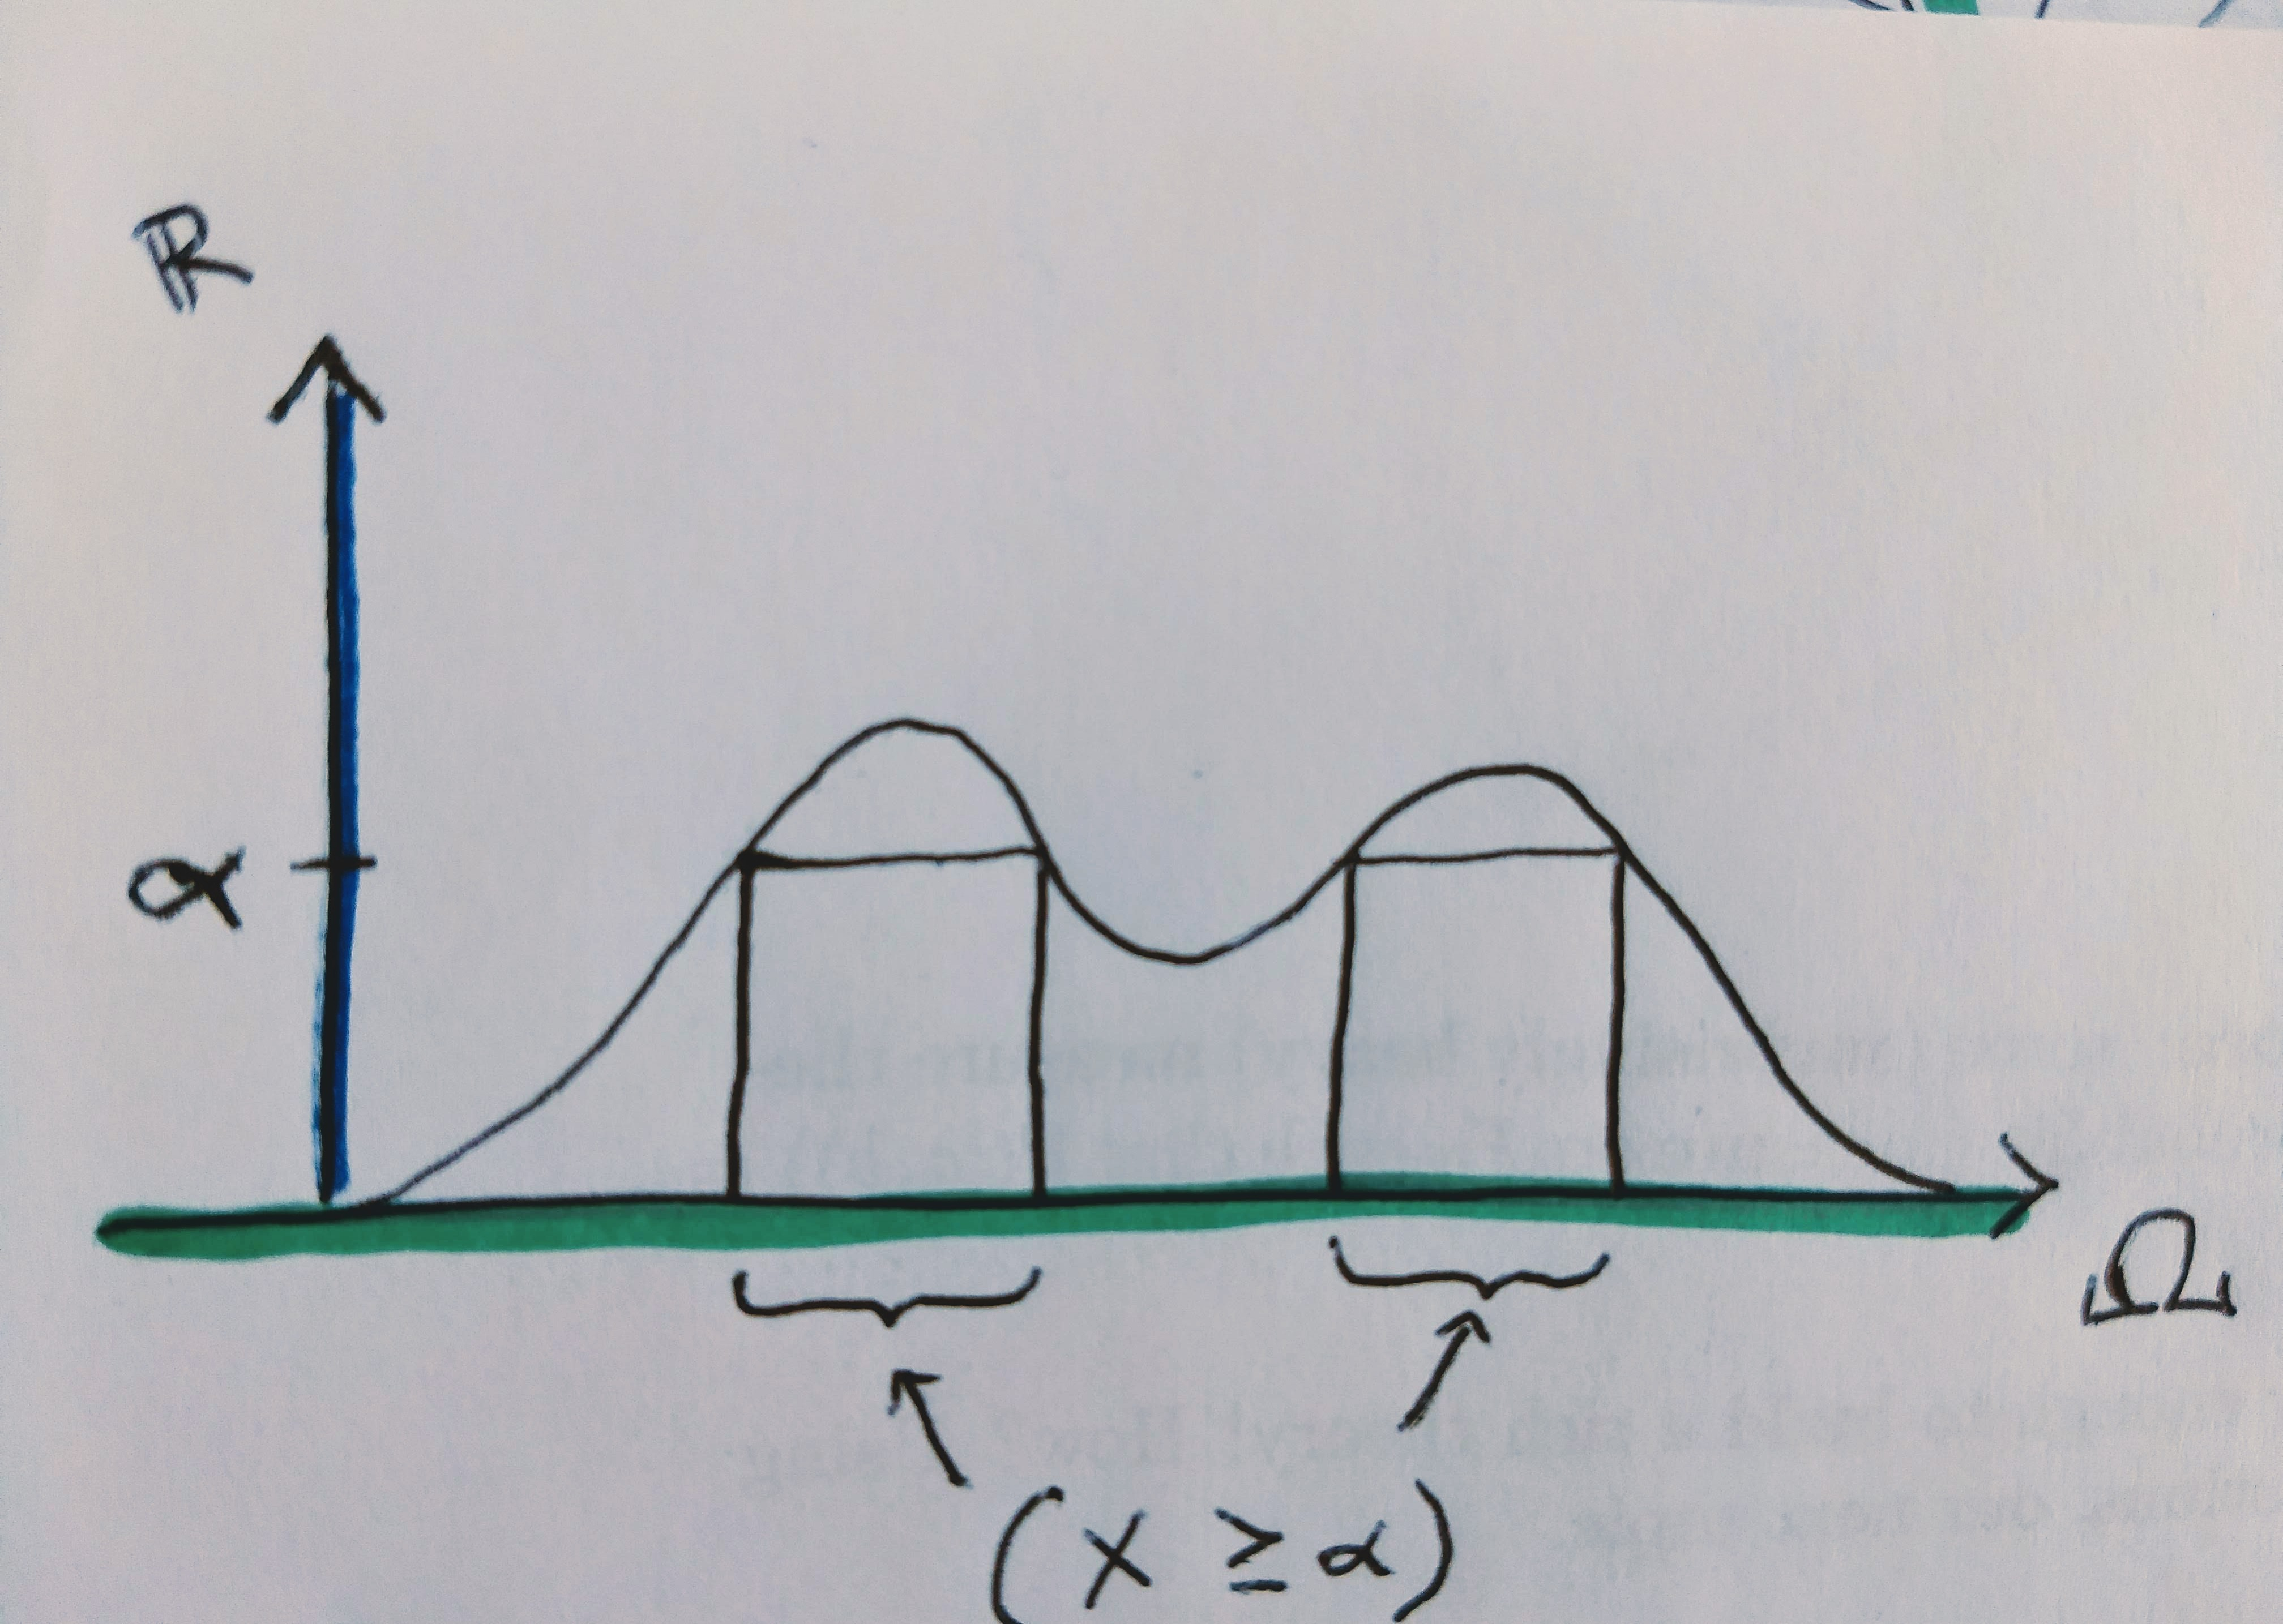
\includegraphics[width=0.5\linewidth]{figures/markov}
\end{center}
Taking expectations on both sides:
\begin{eqnarray*}
\E X &\ge& \alpha \E[\1[X \ge \alpha]] \\
&=& \alpha \P(X \ge \alpha).
\end{eqnarray*}

\point{Note:} non-negativity is necessary. Consider for example a random variable with the discrete uniform distribution on $\{-1, +1\}$, $\alpha = 1$.  

\point{Note:} the bound will sometimes be greater than one. On the other hand, there are random variables $X$ and $\alpha$ such that the bound it tight, i.e. where $\P( X \ge \alpha) = \frac{\E X}{\alpha}$. For example $X$ such that $\P(X = 2) = 1/2$, $\P(X = 0) = 1/2$, $\alpha = 2$.

\point{Corollary 1:} for all random variable $X$, $p \ge 0$,
\[ \P(|X| \ge \alpha) \le \frac{\E |X|^p}{\alpha^p}. \]

\point{Proof:} since the power function is strictly increasing, $(|X| \ge \alpha) = (|X|^p \ge \alpha^p)$. Why? Manipulations of this kind are explained in gory details in the next few section, see specifically \ref{sec:rewriting-equalities} for this step. Therefore $\P(|X| \ge \alpha) = \P(|X|^p \ge \alpha^p)$. Since $|X|^p \ge 0$, we can apply Markov's inequality on this last probability.

% note: does not work well with the dam example because of the left tail

\point{Corollary 2 (Chebyshev's inequality):} for any random variable $Y$ with $\mu \defeq \E Y$, $|\mu| < \infty$ (non-negativity not needed anymore!),
\[ \P(|Y - \mu| \ge \alpha) \le \frac{\var Y}{\alpha^2}. \]

\point{Proof:} define $X \defeq |Y - \mu|$, and apply the preceding lemma with $p = 2$.

\point{Corollary 3 (Chernoff bound):} if $X$ is any random variable, then
\[ \P(X \ge \alpha) \le \inf_t \frac{\E[e^{tX}]}{e^{t\alpha}}. \]

\point{Proof:} For any fixed $t$, the function $f(x) = e^{tx}$ is strictly increasing, so we can use the same reasoning as Chebyshev's. Since the inequality if true for all $t$, the left-hand side is bounded by the infimum over $t$.

\point{Note:} the quantity $\E[e^{tX}]$, viewed as a function of $t$, is called the \emph{moment generating function}. We will meet this object again. 

We will also revisit Chernoff's bound soon once we have introduced independence of random variables. 


\subsection{Rewriting events involving equalities}\label{sec:rewriting-equalities}

This section and the next two provide additional details as well as generalize one of the key step used in the proof of Markov's, Chebyshev's, and Chernoff's inequalities.

Some background: when dealing with equations involving non-random variables, a common heuristic is to ``add on both sides,'' e.g. $x + 5 = 2$ becoming $x = -3$. Let us call these two logical statements $s_1$ and $s_2$. Since $s_1(X(\omega))$ is true if and only if  $s_2(X(\omega))$ is true, it follows that the two events, $(X + 5 = 2)$ and $(X = -3)$, are equal. In particular, $\P(X + 5 = 2) = \P(X = -3)$.

More generally, if $f$ is one-to-one, then $(X = Y) = (f(X) = f(Y))$. For example $(-X = -5) = (X = 5)$. 

In fact, we only need $f$ to be one-to-one on the set of possible values attained by $X$ and $Y$ (i.e. the union of their ranges). For example, if $X$ is non-negative (denoted $X \ge 0$), then $(X = 2) = (X^2 = 4)$. Indeed, even though $f(x) = x^2$ is not one-to-one, it is when restricted to the positive real line.

Many steps in probability arguments follow that kind of logic-based reasoning.


\subsection{Rewriting events involving inequalities}\label{sec:rewriting-inequalities}

Be a bit more careful when dealing with inequalities, we need a more specialized form a one-to-one mapping: if $f$ is \emph{strictly increasing}, then $(X \le Y) = (f(X) \le f(Y))$. For example $(X \le 0) = (\exp(X) \le 1)$.

This is indeed necessary as $(-X \le -5) = (X \ge 5) \neq (X \le 5)$.


\subsection{Bounding events}

When we cannot rewrite the event using the methods described in Sections~\ref{sec:rewriting-equalities} and \ref{sec:rewriting-inequalities}, we can settle on bounding the event instead. Suppose event $A_1$ is defined using statement $s_1(Y)$ (e.g. $A_1 = (Y = 2)$) and similarly, event $A_2$, using $s_2(Y)$ (e.g. $A_2 = (Y^2 = 4)$. Suppose $s_1 \Longrightarrow s_2$. Then we have $A_1 \subseteq A_2$. In our example, $y = 2 \Longrightarrow y^2 = 4$, but the converse is not true if the random variable $Y$ can take negative values, as $y = -2$ also yields $y^2 = 4$. So all we get for general random variables is that $(Y = 2) \subset (Y^2 = 4)$.

Now we have seen in Section~\ref{sec:limit-pr-measures} that $A_1 \subseteq A_2$ implies $\P(A_1) \le \P(A_2)$.


\section{Independence}

\subsection{More than one random variables (random vectors)}\label{sec:random-vectors}

\point{Motivation:} A man and a woman try to meet at a certain place between 1:00pm and 2:00pm.  Suppose each person pick an arrival time between 1:00pm and 2:00pm uniformly at random (denote $X$ and $Y$ respectively), and waits for the other at most 10 minutes. What is the probability that they meet?

\point{Practical question:} How to compute a probability of the form $\P((X, Y) \in S)$?

\point{Theoretical question:} Given two random variables on the same space, $X: \Omega \to \R$ and $Y : \Omega \to \R$, what is $(X, Y)$ exactly?

\point{Definition:} A random vector is a random variable that takes values in $\states = \R^2$: \[ (X, Y) : \Omega \to \R^2. \]

\point{Recall:} The definition of random variable requires a \sigmaalg\ on $\states$. What should we pick? We know that we will at the very least need to compute the probability of $X$ falling in a \emph{rectangle}:

\point{Definition:} a rectangle is a set of the form:
\begin{eqnarray} 
R &=& A \times B \;\text{ for some }A \in \borels, B \in \borels \\
&=& \{(x, y) : x \in A, y \in B\}.
\end{eqnarray}
\begin{center}
	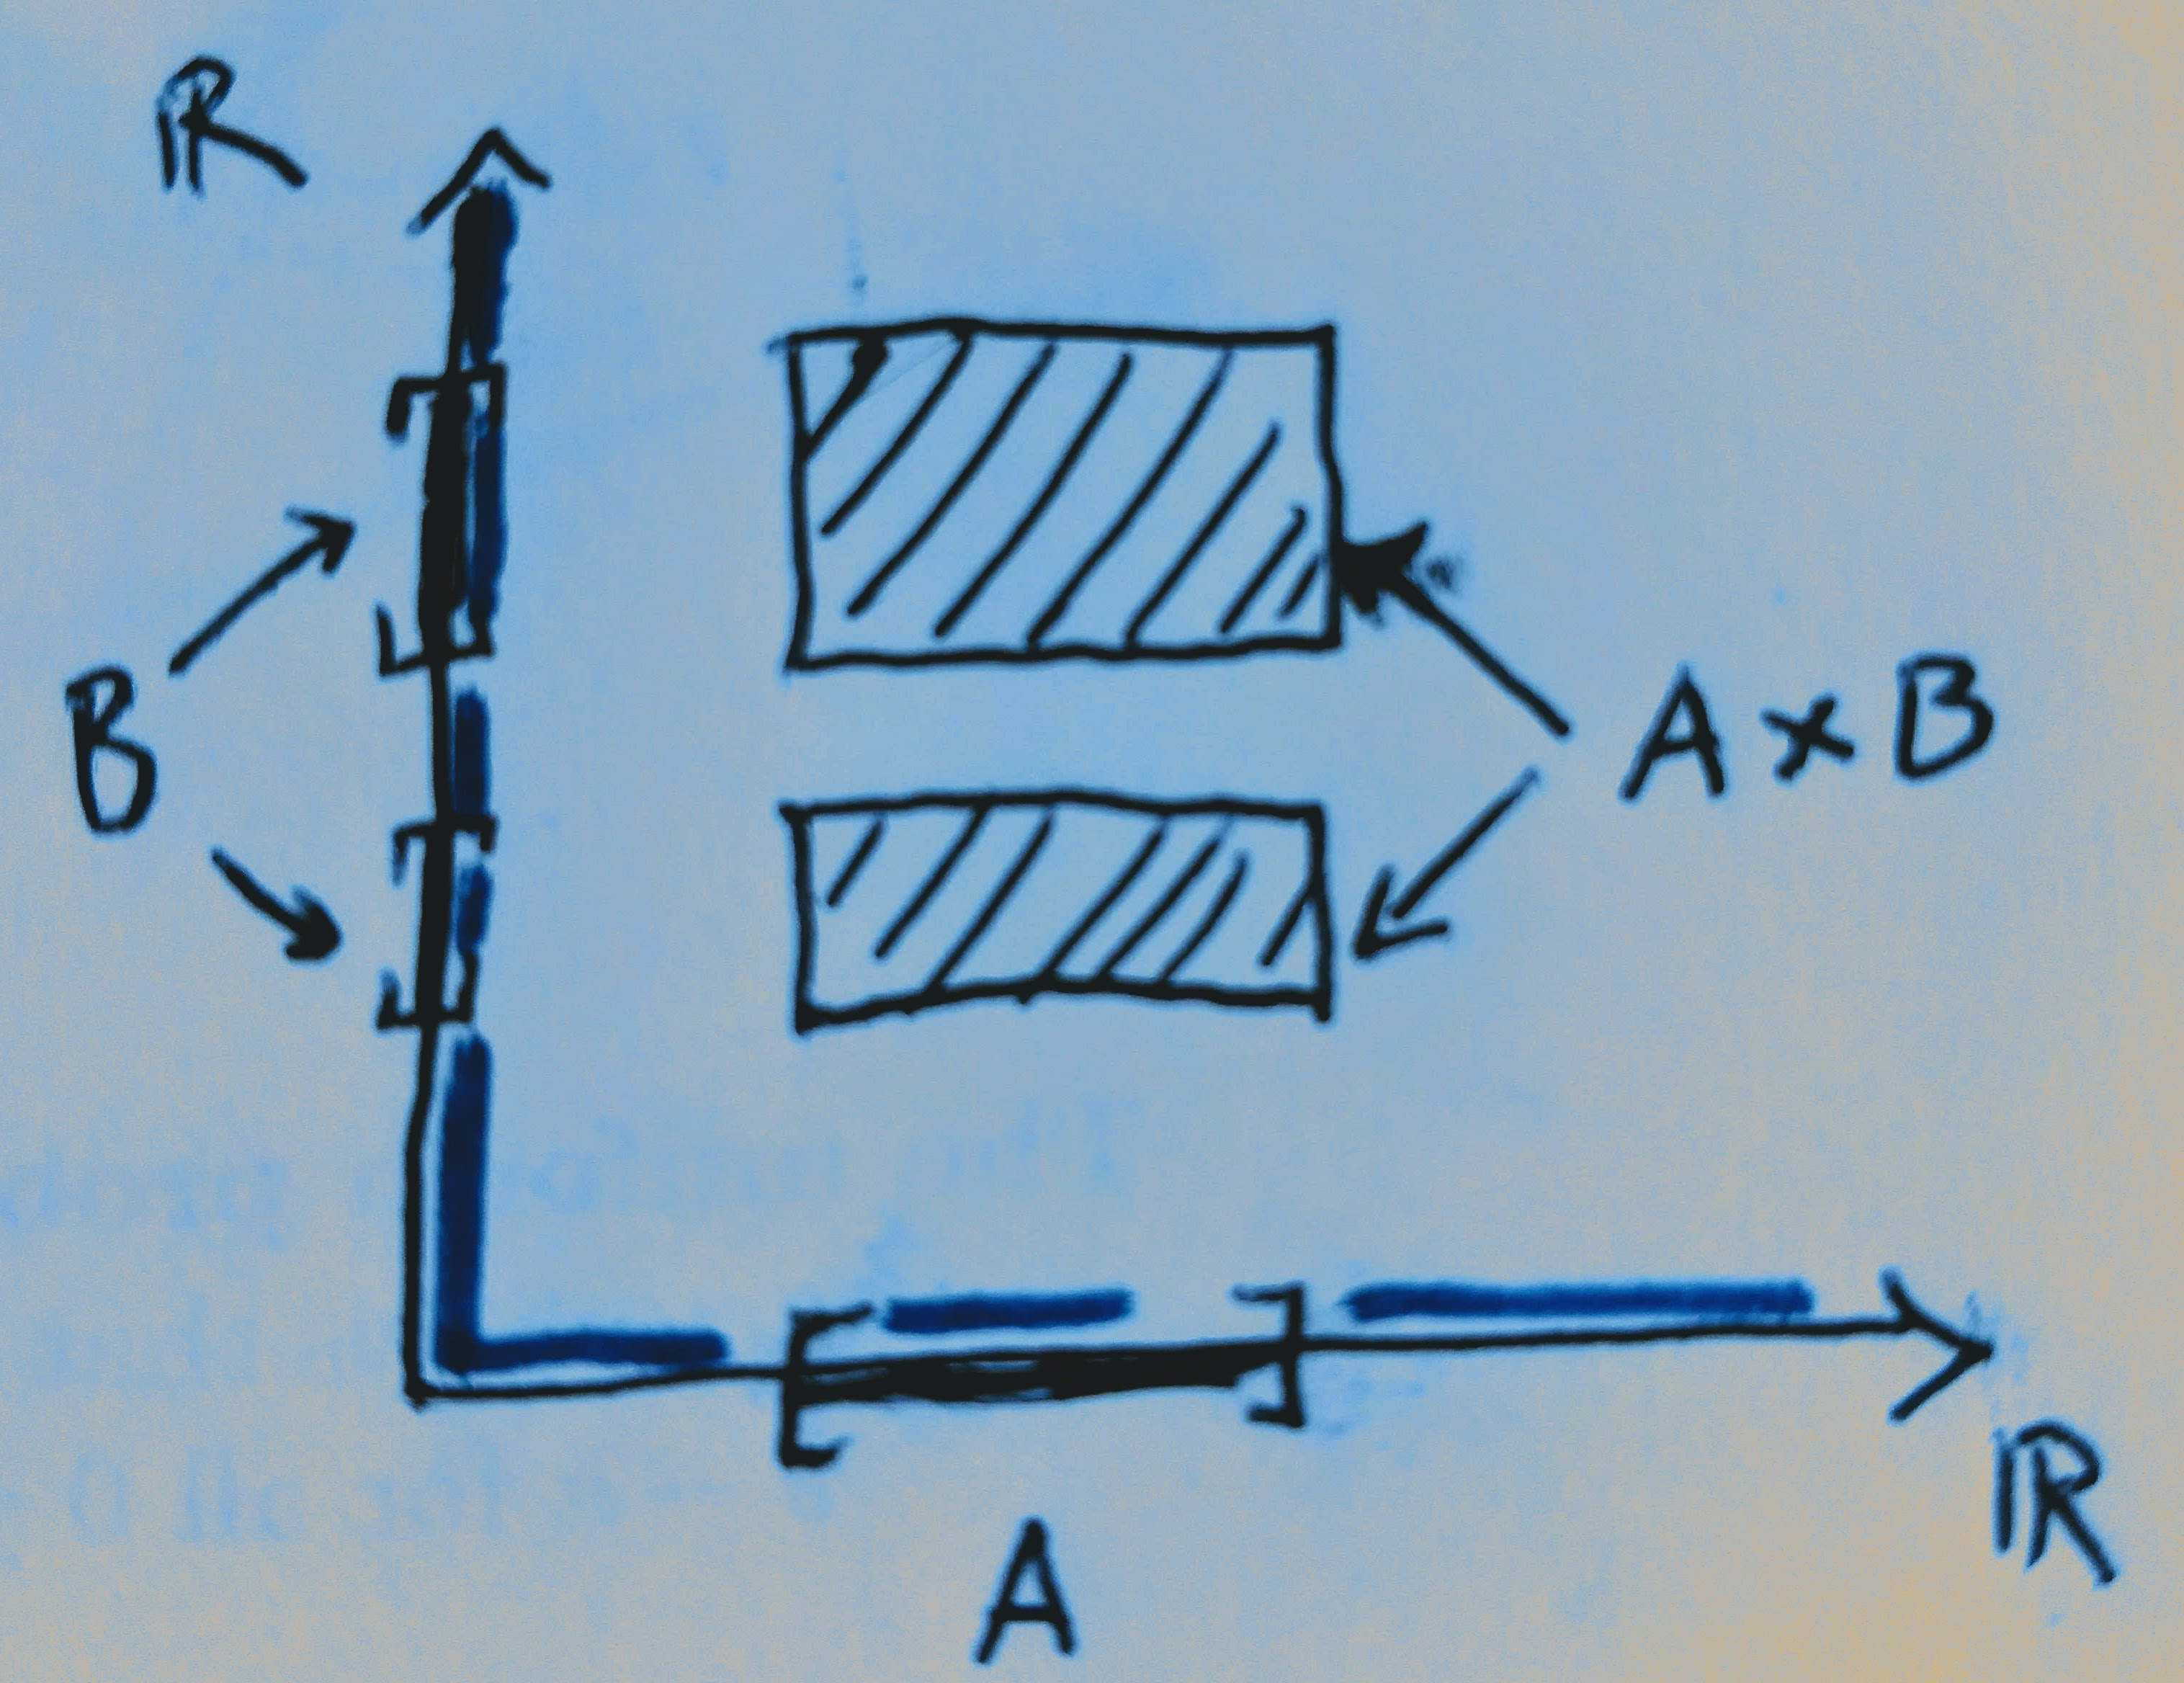
\includegraphics[width=0.4\linewidth]{figures/product}
\end{center}

\point{Unfortunately:} $\generators = \{R : R\text{ is a rectangle}\}$ is not a \sigmaalg\ (why?). Also, it does not contain the set that we would need to answer the ``practical question'' that kicked off this section.
\begin{center}
	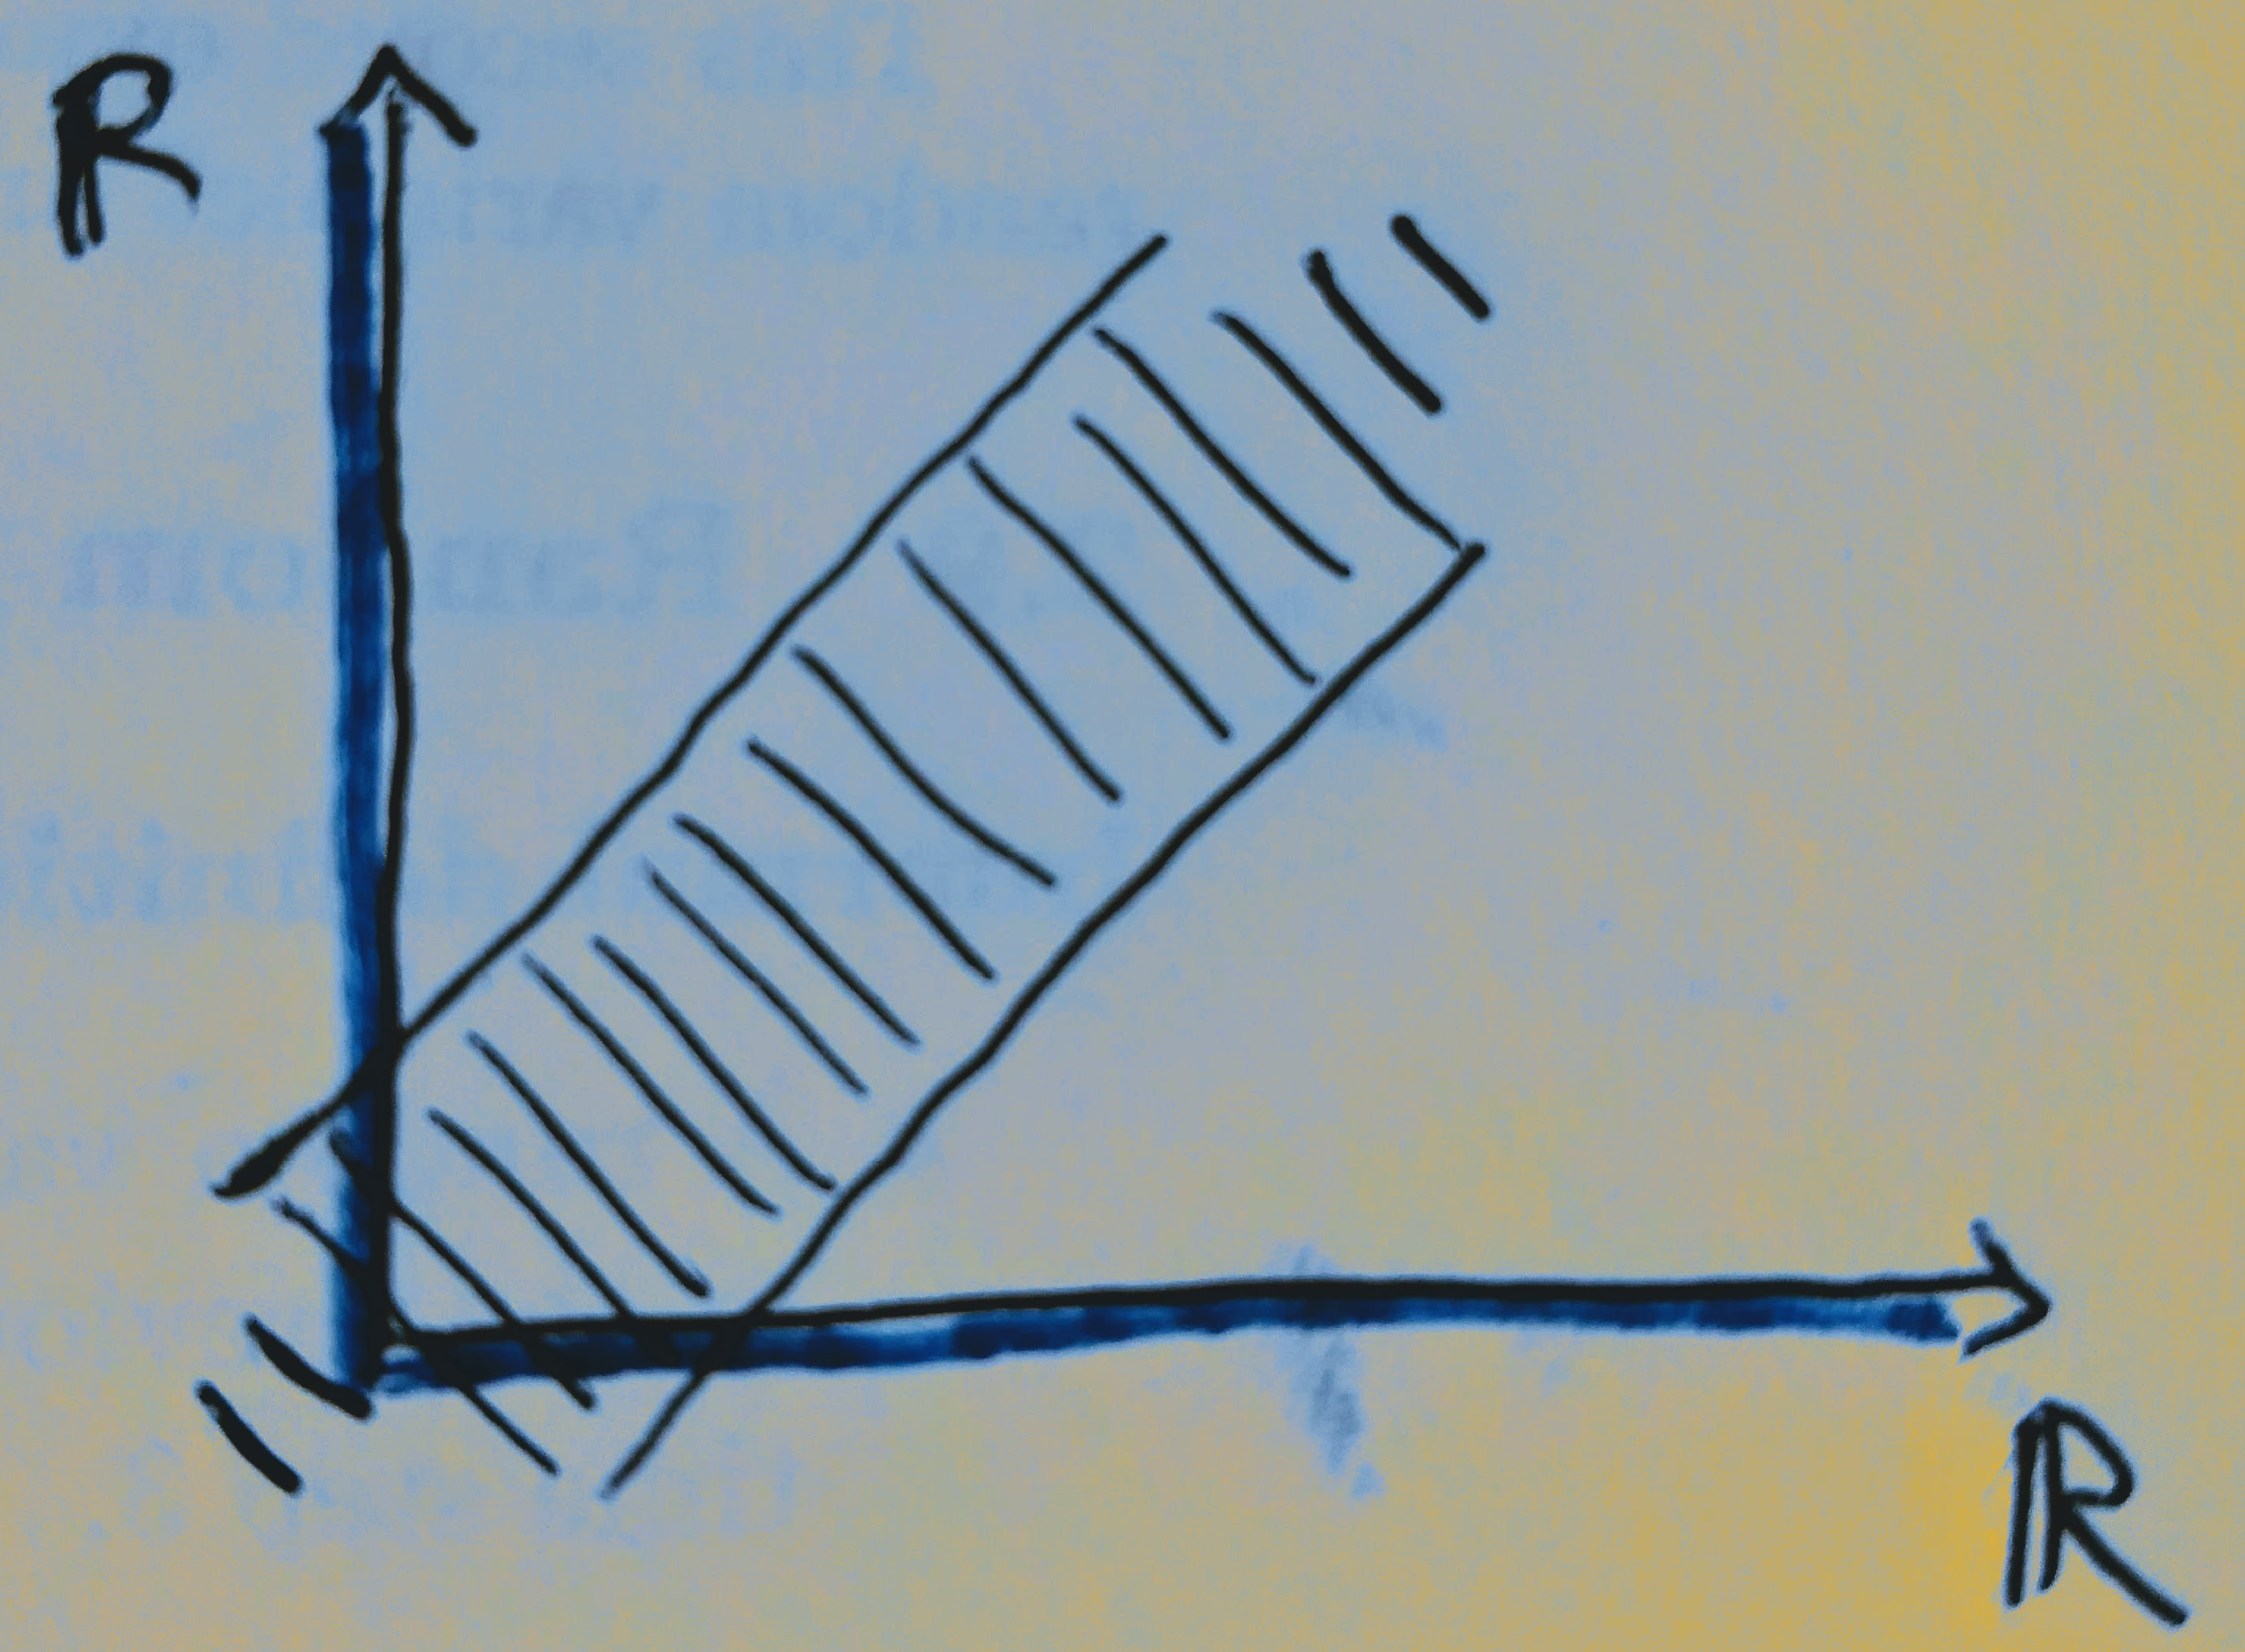
\includegraphics[width=0.4\linewidth]{figures/strip}
\end{center}

\point{Solution:} generate a \sigmaalg\ from $\generators$. The result of this is called the product \sigmaalg:
\[ \events^{\otimes 2} \defeq \events \otimes \events \defeq \sigma(\generators). \]

\point{Exercise:} show that the set $S$ in the ``practical question'' is in $\events \otimes \events$.


\subsection{Distribution, CDF and density of a random vector}

These definitions follow directly from the univariate case:

\point{Definition:} the joint distribution of a random vector $(X, Y)$, denoted $\P_{X,Y} : \events \otimes \events \to [0, 1]$, is defined by:
\[ \P_{X,Y}(S) \defeq \P((X, Y) \in S). \]

\point{Definition:} the joint CDF of a random vector $(X, Y)$, denoted $F_{X,Y} : \R^2 \to [0, 1]$, is defined by:
\[ F_{X, Y}(x, y) \defeq \P_{X,Y}((-\infty, x] \times (-\infty, y]). \]

\point{Note:} This last definition seems slightly arbitrary. Why pick this particular class of sets $S$ (``quarter-planes'')? As we will see in the next section, this is because this class \emph{characterizes} the joint distribution. In other words, given a joint CDF, you can in principle obtain the probability of $X$ falling in any set $S$. 

\point{Definition:} a function $f:\R^2 \to [0, \infty)$ is called a joint density of the random vector $(X,Y)$ if:
\[ F_{(X,Y)}(x,y) = \int_{-\infty}^x \int_{-\infty}^y f(x,y) \ud x \ud y. \]

\point{Note:} these definitions can be generalized to more than two dimensions.


\subsection{Determining classes}\label{sec:determining-classes}

In this section, we explain the tool used to prove the characterization statement of the previous section.

\point{Tool:} $\pi$-$\lambda$ theorem. 
\begin{enumerate}
\item Let $\pi$ denote a collection of sets satisfying the following condition (called a $\pi$-system condition):
\begin{enumerate}
  \item $A, B \in \pi \Longrightarrow A\cap B\in \pi$.
\end{enumerate}
\item Let $\lambda$ denote a collection of sets satisfying the following conditions (called a $\lambda$-system condition):
\begin{enumerate}
  \item $\Omega \in \lambda$,
  \item $A, B \in \lambda, A \subseteq B \Longrightarrow B \backslash A \in \lambda$,
  \item $A_i \uparrow A, A_i \in \lambda \Longrightarrow A \in \lambda.$
\end{enumerate}
\item Then, the following holds: $\pi \subset \lambda \Longrightarrow \sigma(\pi) \subset \lambda$.
\end{enumerate}

\point{Proposition:} Supposet $\P_1$ and $\P_2$ are probability measures on $\events = \sigma(\generators)$, where $\generators$ is closed under finite intersection. Then the following are equivalent:
\begin{enumerate}
  \item $\P_1(A) = \P_2(A)$ for all $A \in \events$,
  \item $\P_1(A) = \P_2(A)$ for all $A \in \generators$.
\end{enumerate}

\point{Exercise:} prove this using the $\pi$-$\lambda$ theorem. Hint: let $\lambda = \{A \in \events : \P_1(A) = \P_2(A)\}$.

\point{Corollary:} $F_{X}$ determines $\P_{X}$.

\point{Proof:} $(-\infty, x] \cap (-\infty, y] = (-\infty, \min\{x, y\}]$. Hence $\generators = \{(-\infty, x]\}$ is a $\pi$ system. Conclude with the $\pi$-$\lambda$ theorem. 

\point{Corollary:} $F_{X,Y}$ determines $\P_{X,Y}$.

\point{Proof:} Use the same proof strategy, this time based on the following picture:
\begin{center}
	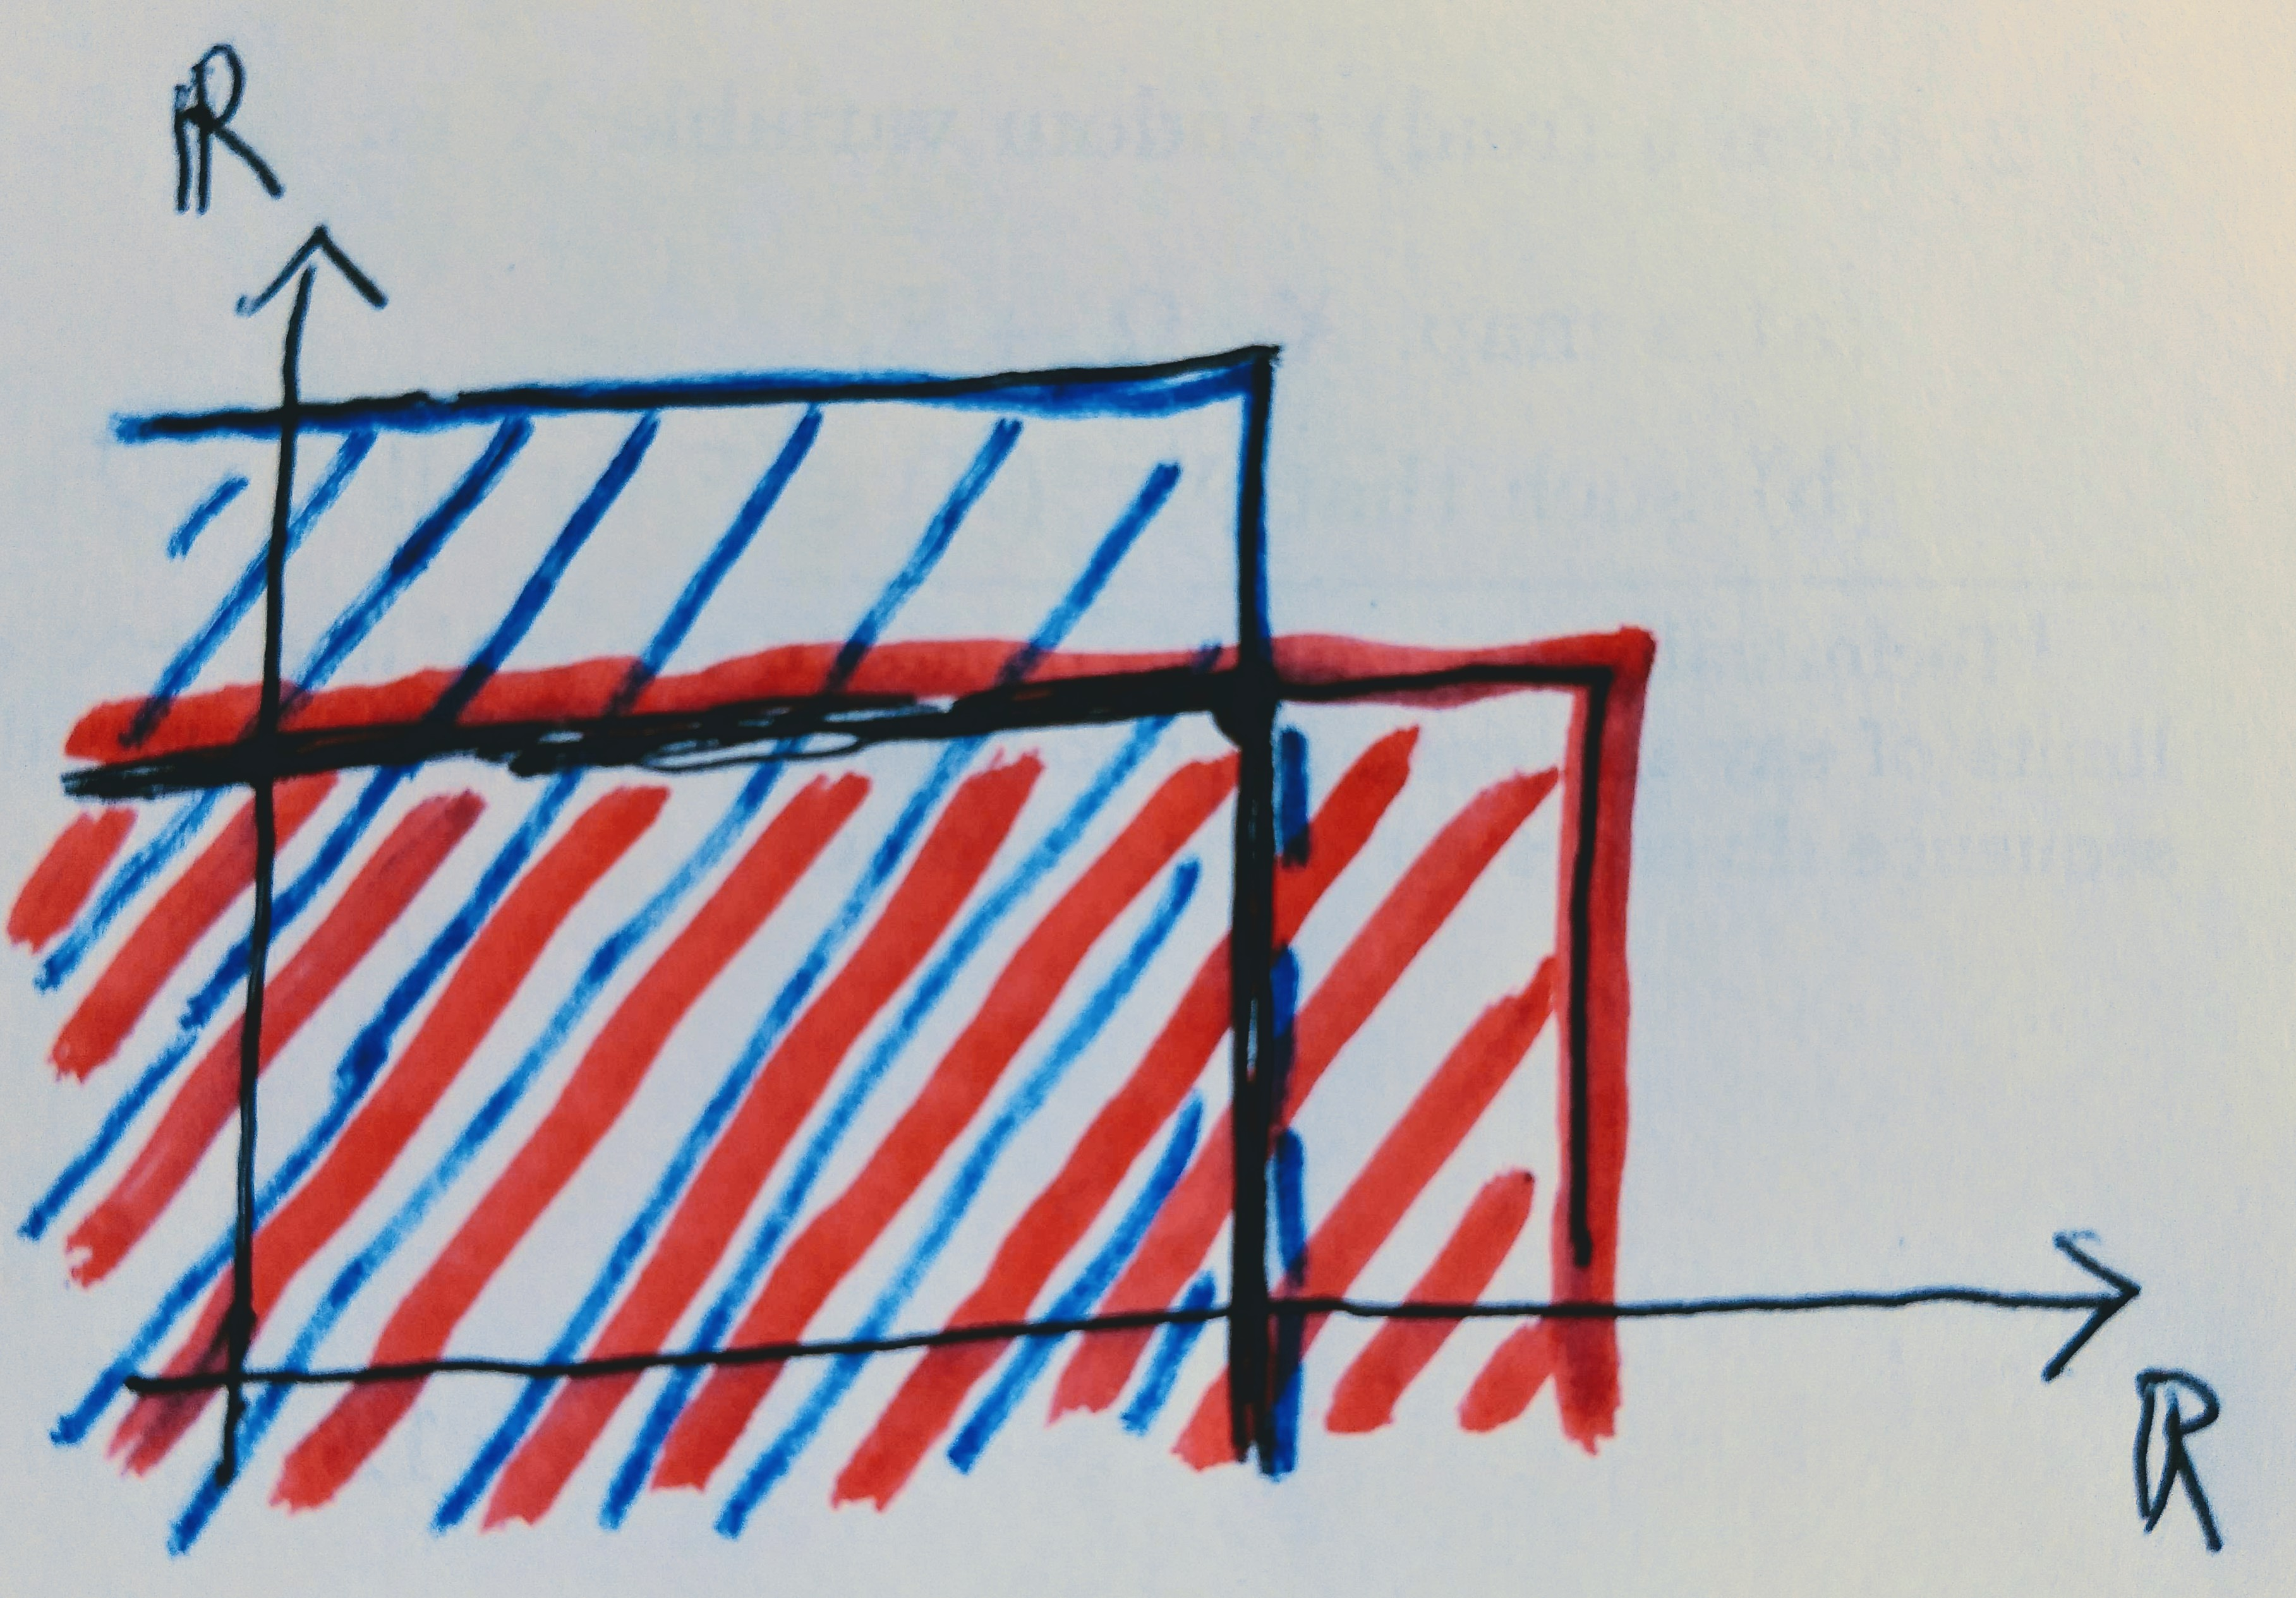
\includegraphics[width=0.5\linewidth]{figures/intersection}
\end{center}

\point{Corollary:} if $(X,Y)$ has joint density $f$, then
\[ \P((X, Y) \in S) = \int_S f(x,y) \ud x \ud y. \]


\subsection{Independence of random variables}

% TODO: come back to Pollards' example of independence to motivate why learning measure theory

\point{Definition:} the random variables $X_1, X_2, \dots, X_n : \Omega \to \R$ are independent if, for all $A_i \in \borels$, \[ \P(X_1 \in A_1, X_2 \in A_2, \dots, X_n \in A_n) = \prod_{i=1}^n \P(X_i \in A_i). \]

\point{Equivalent notation:} \[ \P_{X_1, X_2, \dots, X_n}(A_1 \times A_2 \times \dots \times A_n) = \prod_{i=1}^n \P_{X_1}(A_i). \]

\point{Exercise:} using $\pi-\lambda$ show that the above statement can be checked by showing that the CDF factorizes as 
\[ F_{X_1, X_2, \dots, X_n} = \prod_{i=1}^n F_{X_i}. \]

\point{Note:} similarly to the above exercise, if the random variables have a joint density $f_{X_1, X_2, \dots, X_n}$, independence can be checked by factorizing the density into \emph{marginal densities} $f_{X_i}$ of each individual random variable:
\[ f_{X_1, X_2, \dots, X_n} = \prod_{i=1}^n f_{X_i}. \]

\point{Definition:} we say the random variables $X_1, X_2, \dots, X_n$ are pairwise independent if each pair is independent.

\point{Exercise:} find 3 random variables such that these random variables are pairwise independent but not independent. Hint: this can be done using indicator random variables.


\subsection{Chernoff's bound, continued}\label{sec:chernoff-revisited}

We encountered the moment generating function $f(t) = \E[e^{tX}]$ when talking about Chernoff's bound. When $X$ is a sum of independent random variables, $X = X_1 + X_2 + \dots + X_n$, we get this nice formula:
\[ f(t) = \prod_{i=1}^n f_i(t), \]
where $f_i(t) = \E[e^{tX_i}]$. Informally, adding random variables multiplies their moment generating functions.

Since the moment generating function for individual variables are often easy to compute, this gives a powerful way to evaluate the right hand side of Chernoff's bound 

\point{Example: Chernoff-Hoeffding theorem} if the $X_i$ are independent and each have a Bernoulli($p$) distribution (terminology: ``are iid Bernoulli''), and $\epsilon > 0$:

\begin{align*}
	\P \left (\frac{1}{n} \sum X_i \geq p + \varepsilon \right ) &\leq \left (\left (\frac{p}{p + \varepsilon}\right )^{p+\varepsilon} {\left (\frac{1 - p}{1-p- \varepsilon}\right )}^{1 - p- \varepsilon}\right )^n  \\
	\P \left (\frac{1}{n} \sum X_i \leq p - \varepsilon \right ) &\leq \left (\left (\frac{p}{p - \varepsilon}\right )^{p-\varepsilon} {\left (\frac{1 - p}{1-p+ \varepsilon}\right )}^{1 - p+ \varepsilon}\right )^n 
\end{align*}

\point{Proof:} compute the moment generating function of a Bernoulli. Then use calculus to minimize over $t$. Then plug-in the minimum. Use the variable $Y_i = 1 - X_i$ to establish the other side of the bound.

\point{Other versions:} see the wikipedia page for many more bounds derived from this.  


\subsection{Exercise set 3}

\begin{enumerate}
	\item Exercise in Section~\ref{sec:area-simple-function} about  linearity in the case of simple functions.
	\item Solve the two exercises in Section~\ref{sec:convexity}.
	\item Motivating exercise in Section~\ref{sec:markov}.
	\item Exercise in Section~\ref{sec:determining-classes}.
\end{enumerate}


\subsection{Solutions for exercise set 3}\label{sec:sol-ex-iii}
\begin{enumerate}
	\item Let $Y=\sum_{i=1}^Na_i\1_{A_i}$ and $Y'=\sum_{j=1}^Mb_j\1_{B_j}$ for $\{A_i\}_{i=1}^N, \{B_j\}_{j=1}^M$ are measurable disjoint collections. Notice that since $\{A_i\}_{i=1}^N$ and $\{B_j\}_{j=1}^M$ are disjoint, we have
	\[\1_{A_i}=\sum_{j=1}^M1_{A_i\cap B_j},\quad \1_{B_j}=\sum_{i=1}^N1_{A_i\cap B_j}.\]
	Therefore, $Y+Y'$ can be written as
	\begin{align*}
	Y+Y'
	&=\sum_{i=1}^Na_i\1_{A_i}+\sum_{j=1}^Mb_j\1_{B_j}\\
	&=\sum_{i=1}^Na_i\sum_{j=1}^M1_{A_i\cap B_j}+\sum_{j=1}^Mb_j\sum_{i=1}^N1_{A_i\cap B_j}\\
	&=\sum_{i=1}^N\sum_{j=1}^M(a_i+b_j)1_{A_i\cap B_j}.
	\end{align*}	
	Since $A_i\cap B_j$ are disjoint, we have $Y+Y'$ is a simple function and by the definition of the expectation,
	\begin{align*}
	\E[Y+Y']
	&=\sum_{i=1}^N\sum_{j=1}^M(a_i+b_j)\P(A_i\cap B_j)\\
	&=\sum_{i=1}^Na_i\sum_{j=1}^M\P(A_i\cap B_j)+\sum_{j=1}^Mb_j\sum_{i=1}^N\P(A_i\cap B_j)\\
	&=\sum_{i=1}^Na_i\P(A_i)+\sum_{j=1}^Mb_j\P(B_j)\\
	&=\E[Y]+\E[Y'].
	\end{align*}
	
	\item 
		\begin{enumerate}
		\item Let $\Omega=[0,1]$ with $\P$ be the Lebesgue measure and $X:\Omega\to\R$ be the identity. If $\varphi:\R\to\R$ be $\varphi(x)=x^2$. Then,
		\begin{align*}
		\E(X)=\int_{[0,1]}x\P(dx)=\int_0^1xdx=\frac{1}{2},
		\end{align*}
		and similarly,
		\begin{align*}
		\E(X^2)=\int_{[0,1]}x^2\P(dx)=\int_0^1x^2dx=\frac{1}{3}.
		\end{align*}
		Therefore $\varphi(\E [X])=1/4$ which does not equal $\E[\varphi(X)]=1/3$.
		
		\item Let $\varphi=\1_{\{0\}}$. Suppose that there is a sequence of linear functions $L_n(x)=a_nx+b_n$ such that $\sup_n L(x)=\varphi(x)$ for all $x$. Suppose that $a_{n_0}\neq 0$ for some $n_0$. Then $L_{n_0}$ is unbounded from above and there is some $x_0\in \R$ such that $L_{n_0}(x_0)=2$. Thus $\sup_n L_n(x_0)\geq 2>\varphi(x_0)$ which is a contradiction. Thus we have all $a_n=0$.\\
		\newline
		For $x\neq 0$, we have $\varphi(x)=0=\sup_n L_n(x)=\sup_n b_n$, which implies $b_n\leq 0$ for all $n$. However when $x=0$, and $\sup_n L_n(0)=\sup_n b_n\leq 0\neq 1 \varphi(x)$. \\
		\newline
		Thus we have shown there does not exist a sequence of linear  functions $L_n$ such that $\sup_n L(x)=\varphi(x)$ for all $x$.
		\end{enumerate}
	\item There is a flood when the water level $X$ is higher than the dam, which is at 7.5m. By Markov's inequality,
	\begin{align*}
	\P(\text{Flood})=\P(X\geq 7.5)\leq \frac{\E X}{7.5}=\frac{5}{7.5}=\frac{2}{3}.
	\end{align*}
	Therefore a flood will occur with maximum probability 2/3.
	
	\item ``$(1)\rightarrow (2).$'' This follows trivially since $\mathcal{S}\subset\mathcal{F}$.\\
	\newline
	``$(2)\rightarrow (1).$'' As suggested by the hint, we define 
	\[\lambda=\{A\in\mathcal{F}:\P_1(A)=\P_2(A)\}.\]
	We will now show that $\lambda$ is a $\lambda$-system:
	\begin{enumerate}
		\item [1.] Note that $\P_1(\Omega)=1=\P_2(\Omega)$, thus $\Omega\in \lambda$.
		\item [2.] Suppose $A,B\in\lambda$ and $A\subset B$. We then have,
			\begin{eqnarray*}
			\P_1(B\backslash A)&=&\P_1(B)-\P_1(A) \\
			&=& \P_2(B)-\P_2(A) \;\text{(since }A,B\in\lambda) \\
			&=& \P_2(B\backslash A).
			\end{eqnarray*}
		\item [3.] Suppose $A_i\uparrow A$ for all $A_i\in\lambda$. Then
			\begin{eqnarray*}
			\P_1(A)&=&\lim_{i\to\infty} \P_1(A_i) \;\text{(continuity of measures}) \\
			&=& \lim_{i\to\infty}\P_2(A_i) \;\text{(since }A_i\in\lambda) \\
			&=&\P_2(A) \;\text{(continuity of measures}). \\
			\end{eqnarray*}
	\end{enumerate}
	Therefore we have shown that $\lambda$ is a $\lambda$-system. Since $\mathcal{S}$ is closed under finite intersection, we have by definition it is a $\pi$-system. Thus by the $\lambda-\pi$ theorem $\mathcal{F}=\sigma(\mathcal{S})\subset\lambda$, which completes the proof.
\end{enumerate}



\section{Computing expectations in practice}

\subsection{Computing integrals using calculus}\label{sec:calculus}

When $\Omega = [a, b] \subset \R$, $\mu$ is uniform, and $f$ is bounded, then the Lebesgues integral $\int f \ud \mu$ behaves in the same way as the standard Riemann integral (as long as the latter exists, which is true iff the set of discontinuities of $f$ have measure zero). Hence you can in principle use the \point{fundamental theorem of calculus} to compute these integrals: if there is a function $F$ such that $F'(x) = f(x)$ for all $x \in \Omega$, then 
\[ \int f \ud \mu = \int f(x) \ud x = F(b) - F(a). \]
It also follows that $F$ is the \CDF\ of $X$.  

The limitation of this approach is that even when $f$ is a simple close-form expression (expressed in terms of $+, -, *, /, \exp, \log$), the CDF $F$ might not have such a close-form expression (example: $f(x) = \exp(-x^2)$).


\subsection{Computing expectations using the distribution of the random variable}\label{sec:change-of-var}

\point{Motivating example:} consider a space $\Omega$ containing the following four objects: a circle, a triangle, a square, and a pentagon, and a probability $\P$ that give then equal probabilities (1/4). Let $X$ denote a random variable that takes a shape as input and output the number of faces. Suppose we want to compute $\E[g(X)]$, where $g(x) = \1[x \text{ is an even integer}]$. We will see two methods for doing this:

\point{From the definition:} let $Y = g(X)$. We see that $Y$ can take two possible values, zero and one, therefore it is simple. Applying the definition of expectation of simple function:
\begin{eqnarray*} 
\E[Y] &=& \int Y \ud \P \\
&=& 1\times \P(Y = 1) + 0\times \P(Y = 0) \\
&=& \P(Y^{-1}(\{1\}) \\
&=& \P(X^{-1}(g^{-1}(\{1\}))) = 1/2.
\end{eqnarray*}

\point{Another way:} first, derive the distribution of $X$:
\[ \P_X(A) = \frac{1}{4}\left( \1[0 \in A] + \1[3 \in A] + \1[4 \in A] + \1[5 \in A] \right). \]
then, compute an integral of $g$ \emph{with respect to the distribution of $X$}:
\[ \int g \ud \P_X. \]
Here, $g$ is an indicator, so it is a simple function, so we can use our definition of integral of simple functions:
\begin{eqnarray*}
\int g \ud \P_X &=& 1 \times \P_X(\{x : g(x) = 1\}) + 0 \times \P_X(\{x : g(x) = 0\}) \\
&=& \P_X(\{\dots, -6, -4, -2, 0, 2, 4, 6, \dots\}) \\
&=& 1/2.
\end{eqnarray*}

\point{Proposition (``change of variable''):} these two methods are equivalent. More precisely, if $Y = g(X)$ is a random variable and either $g \ge 0$ or $Y \in \L_1$, then:
\[ \int Y \ud \P = \int g \ud \P_X. \]

\point{Note:} by ``either $g \ge 0$ or $Y \in \L_1$'' I mean that the above can actually be slit into two propositions, one assuming the first condition, and a second proposition assuming the second condition.

\point{Note:} an important special case is $g(x) = x$.

\point{Note:} the nice thing with the second way is that you do not have to know $\Omega$ and $\P$, which are often not explicitly given to you. Often all I tell you is $X \sim F$, which characterizes $\P_X$, and I ask $\E[g(X)]$. Using our proposition we can solve this using an integral over the real line with a measure on the reals provided by $\P_X$.

\point{Proof:} assume first that $g = \1_A$. From the same computation as in the example above, we have on one hand:
\[ \int Y \ud \P = \P(Y = 1), \]
and on the other hand:
\begin{eqnarray*} 
\int g \ud \P_X &=&  \P_X(\{x : g(x) = 1\}) \\
&=& \P(X \in \{x : g(x) = 1\}) \\
&=& \P(g(X) = 1) \\
&=& \P(Y = 1).
\end{eqnarray*}

\noindent Next, assume $g$ is simple, i.e. $g = a_1 \1_{A_1} + \dots + a_n \1_{A_n}$. We have:
\begin{eqnarray*}
\int g(X) \ud \P &=& \int \sum_i a_i \1_{A_i}(X) \ud \P \\
&=& \sum_i a_i \int \1_{A_i}(X) \ud \P \;\text{ (using linearity)} \\
&=& \sum_i a_i \int \1_{A_i} \ud \P_X \;\text{ (using first part of proof)}\\
&=& \int \left(\sum_i a_i \1_{A_i}\right) \ud \P_X\;\text{ (using linearity)} \\
&=& \int g \ud \P_X.
\end{eqnarray*}

\noindent Third, assume $g \ge 0$ (or $g\in \L_1$). Use the approximation theorem to get $g_i \uparrow g$, so that:
\begin{eqnarray*}
\int g(X) \ud \P &=& \int \lim g_i(X) \ud \P \\
&=& \lim \int g_i(X) \ud \P \;\text{(using MCT (or DCT))} \\
&=& \lim \int g_i \ud \P_X \;\text{(using second part of proof)} \\
&=& \int \lim g_i \ud \P_X \;\text{(using MCT)} \\
&=& \int g \ud \P_X.
\end{eqnarray*}.


\subsection{How probability spaces and random variables are constructed in practice}\label{sec:using-rv-to-construct-prs}

So far we have often insisted in explicitly constructed $\Omega$, $\events$, $\P$, and designed random variables $X$ by providing, for each $\omega$, the value $X(\omega)$. This level of detail is useful for certain proofs (e.g. Markov's inequality), but for many day-to-day calculations, it is not necessary to go into that much detail. 

\point{Idea:} instead of defining $\Omega$, $\events$, $\P$ and $X$, just specify the distribution of $X$. I.e. say something like ``let $\Omega$, $\events$, $\P$ and $X$ be such that $X \sim \Bern(p)$, i.e. such that $X$ has a Bernoulli $p$ distribution.'' 

\point{How do we know that there are such $\Omega$, $\events$, $\P$ and $X$?} Thanks to the inverse CDF construction, introduced in Section~\ref{sec:inverse-cdf}. 

\point{This does not uniquely define $\Omega$, $\events$, $\P$ and $X$:} recall from Section~\ref{sec:equal-in-distribution} that there are several ways to build $\Omega$, $\events$, $\P$ and $X$ that yield the same distribution on $X$.

\point{However:} in light of the preceding Section (\ref{sec:change-of-var}), we only need the distribution in order to compute arbitrary expectations. So even though $\Omega$, $\events$, $\P$ and $X$ are not technically fully specified, they are constrained enough for our purpose.

For this reason, often we do not even mention $\Omega$, $\events$, $\P$, and just assume there is a ``global'' probability space on which the random variables are defined based on their distributions. 


\subsection{Computing expectations using densities}

\point{Generalization of density:} we say $X$ has a density $f$ with respect to $\mu$ (typically, $\mu$ is the uniform measure on $\R$, but other choices are possible), if:
\[ \P_X(A) = \int \1_A f \ud \mu \;\;\text{ for all }A\in\borels. \]

\point{Note:} this generalizes our previous definition of density given in Section~\ref{sec:density-first-def}:
\begin{eqnarray*} 
F_X(b) - F_X(a) &=& \P_X([a, b]) \\
&=& \int_a^b f(x) \ud x \;\text{ (by Section~\ref{sec:calculus})}
\end{eqnarray*}
Therefore by letting $a \to -\infty$ we recover the formula from Section~\ref{sec:density-first-def}.

\point{Critical question in first assignment:} show that if $g \ge 0$ or $g \in \L_1$, 
\[ \E[g(X)] = \int f(x) g(x) \mu(\ud x). \]

\point{Why this is useful:} because we can now compute expectations using calculus, even when $\Omega \neq \R$, and by knowing only $\P_X$.


\subsection{Computing the expectation of a function of independent random variables}\label{sec:expectation-indep}

\point{Motivation:} back to the motivating problem of Section~\ref{sec:random-vectors}. How to formalize the compution of the expectation, $\E[\1[|X-Y| \le 1/6]]$. Let us define $g(x,y) \defeq \1[|x-y| \le 1/6]$. By our change of variable formula (Section~\ref{sec:change-of-var}), \[ \E[ g(X,Y) ] = \int g \ud \P_{X,Y}. \]

Now our independence assumption on the arrival times of the woman and man means that $\P_{X_1,X_2}(A_1 \times A_2) = \P_{X_1}(A_1) \P_{X_2}(A_2)$. To solve this last integral, we use this independence statement and the following theorems:

\point{Tonelli:} if $g \ge 0$, and $\mu \times \mu$ is such that $\mu \times \mu(A_1 \times A_2) = \mu_1(A_1) \mu_2(A_2)$ (think of $\mu_1$ and $\mu_2$ as the marginal distributions of two \emph{independent} random variables, i.e. $\mu \times \mu$ as $\P_{X,Y}$, $\mu_1$ as $\P_X$ and $\mu_2$ as $\P_Y$), then:
\begin{eqnarray*}
\int g \ud(\mu_1 \times \mu_2) &=& \int \left( \int g \ud \mu_1 \right) \ud \mu_2 \\
&=& \int \left( \int g \ud \mu_2 \right) \ud \mu_1,
\end{eqnarray*}
in other words, we can approach the problem as iterated univariate integrals, and do so in any order we wish.

\point{Fubini:} same statement as Tonelli, but instead of requiring $g \ge 0$, we ask that $\int |g| \ud(\mu_1 \times \mu_2) < \infty$. How to check this ${\L}_1$ condition? By first applying Tonelli on $|g| \ge 0$!

\noindent Being able to write joint integrals as iterated ones is nice because the inner integral is just over the real line, so we can use our density $f$ of $X_1$ and calculus at this point.

\point{Corollary:} $X$ and $Y$ are independent if and only if for all measurable $g_i \ge 0$, \[ \E[g_1(X) g_2(Y) ] = \E[g_1(X)] \E[g_2(Y)]. \]

\point{Solving the meeting problem:} by Fubini, we have
\[ \int g \P_{X,Y} = \int \left( \int g \ud \P_X \right) \ud \P_Y. \]
Now the inner integral can be rewritten as an integral over $[0, 1]$ using the density question in the first assignment:
\[ \int \left( \int g \ud \P_X \right) \ud \P_Y = \int \left( \int f(x) g(x,y) \ud x \right) \ud \P_Y, \]
where $f(x)$ is the uniform density over $[0, 1]$, $f(x) = \1_{[0, 1]}(x)$. Applying the same argument to the outer integral, we get:
\[ \int \left( \int f(x) g(x,y) \ud x \right) \ud \P_Y = \int f(y) \int f(x) g(x,y) \ud x \ud y, \]
which is the area of the dashed region in the following figure: 
\begin{center}
	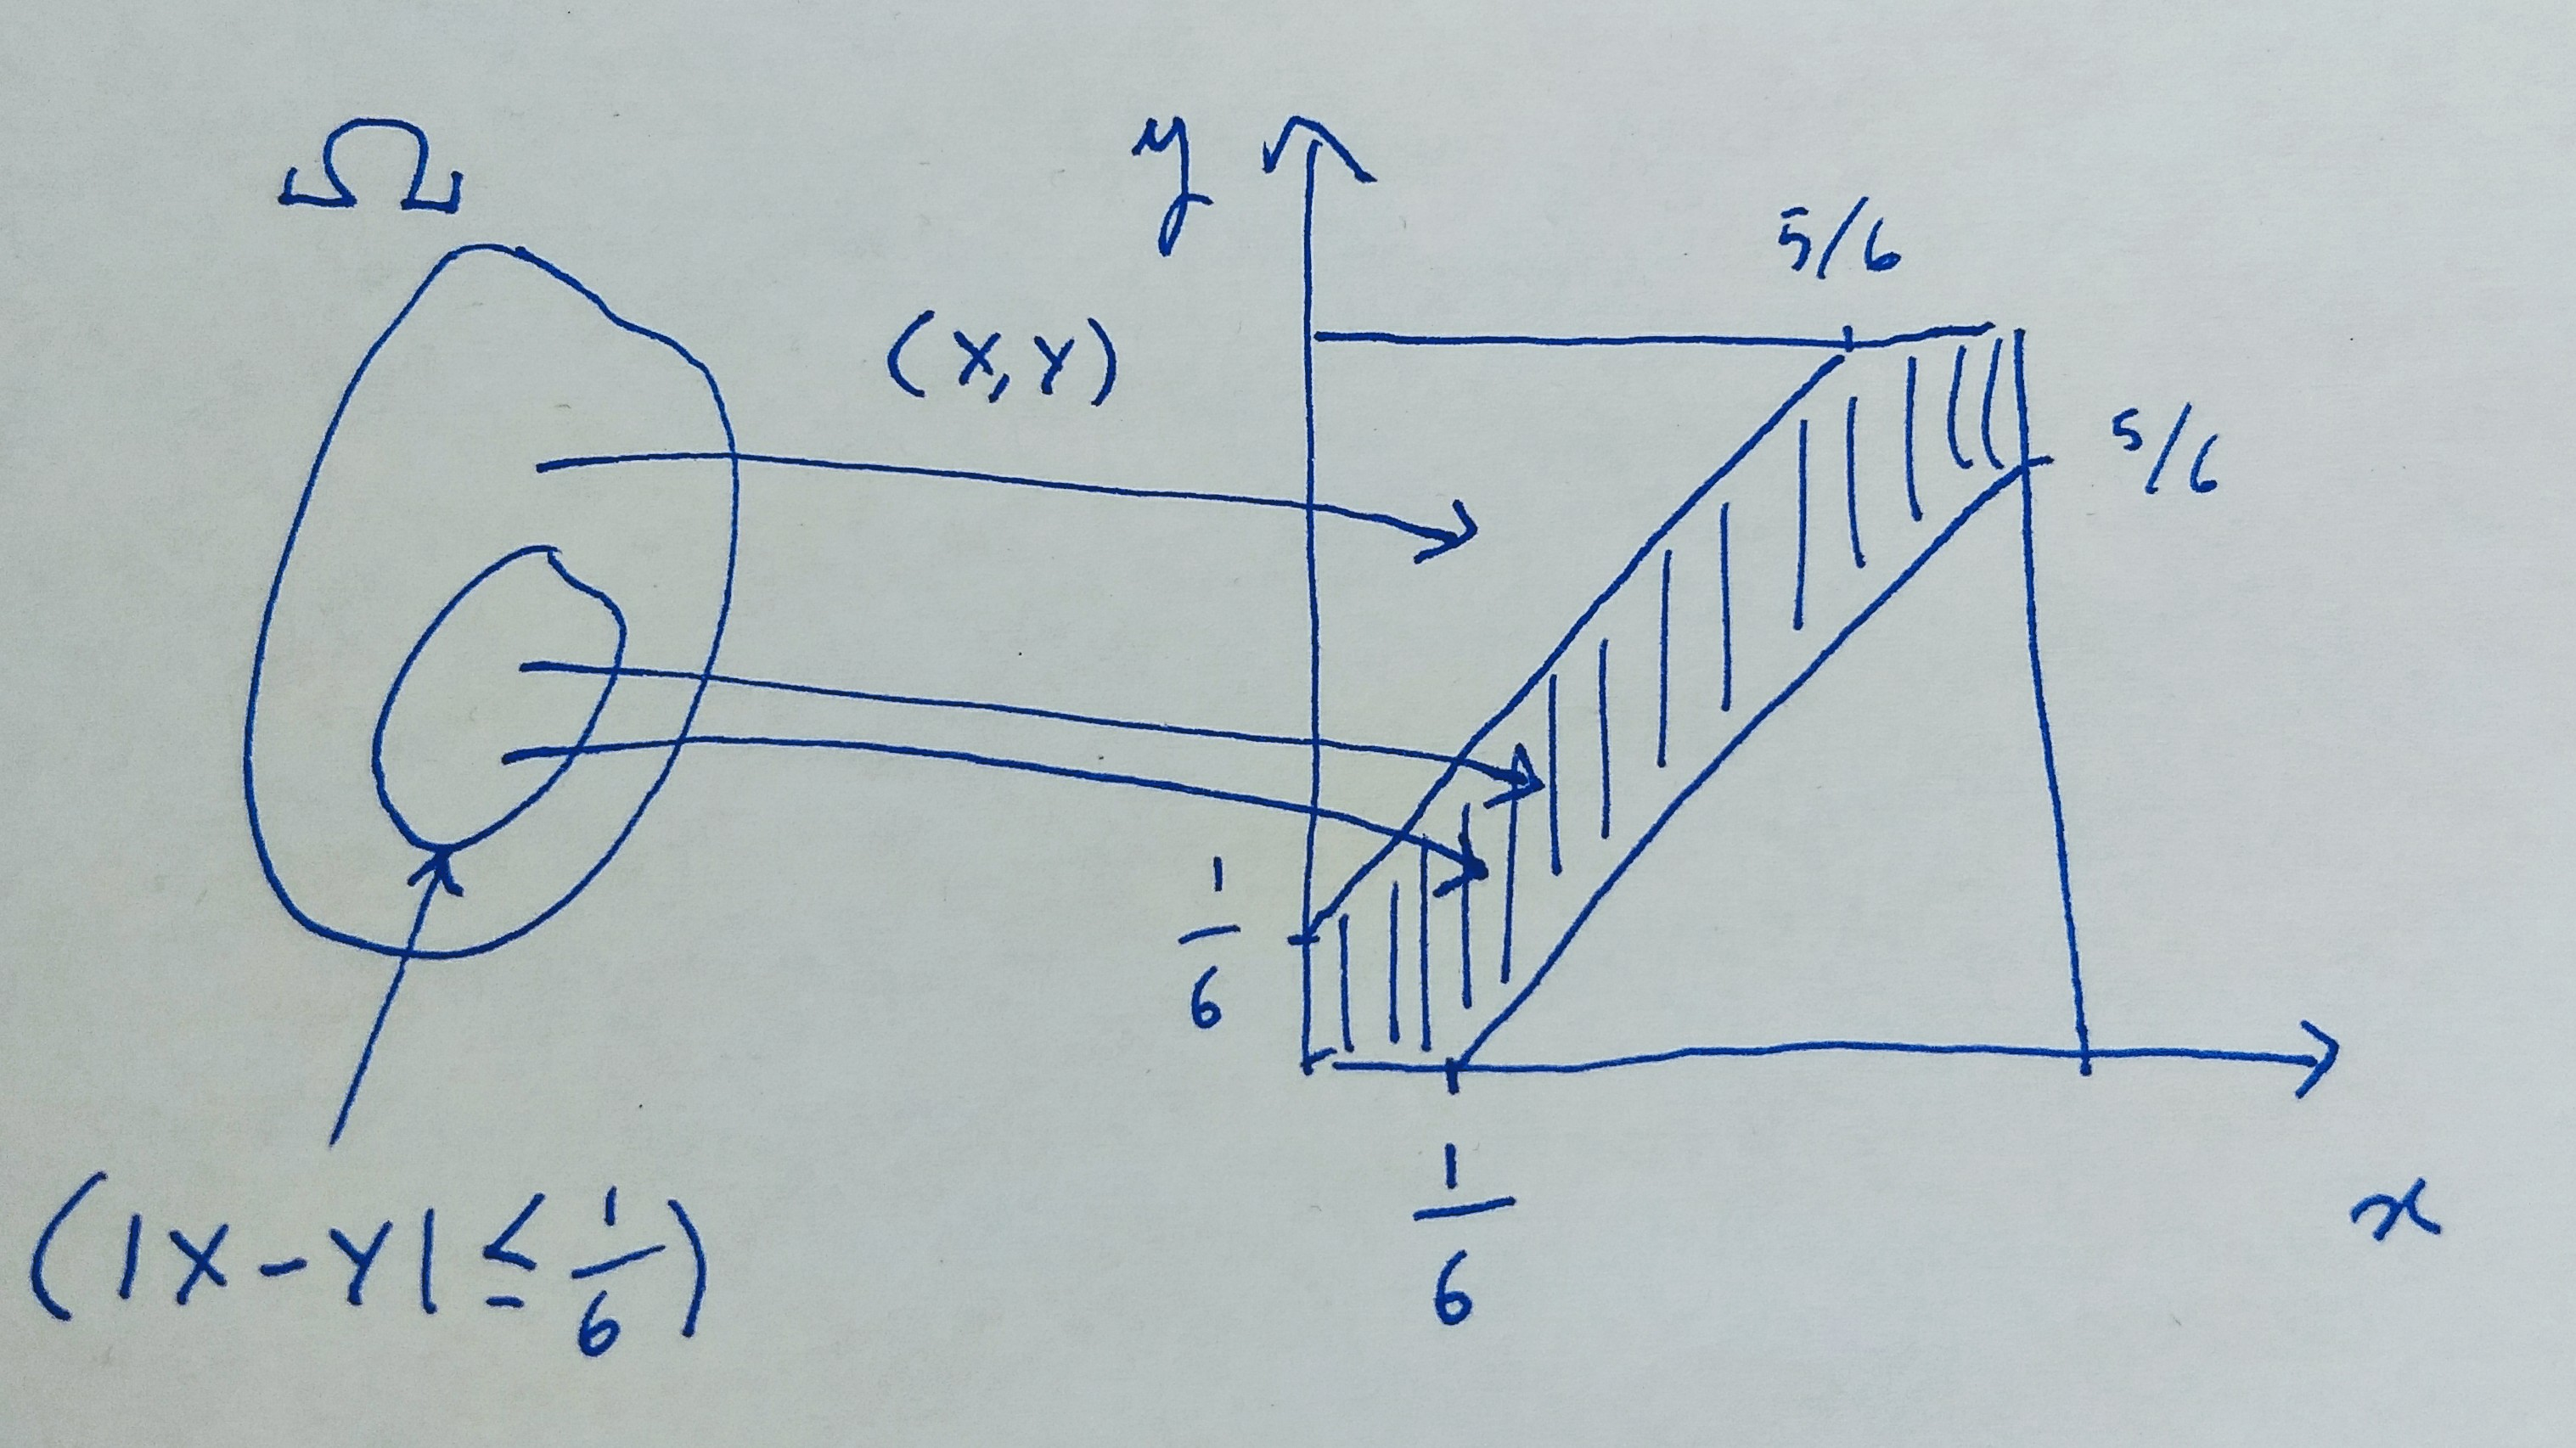
\includegraphics[width=0.5\linewidth]{figures/meeting}
\end{center}

\point{Important:} the notion of \emph{independent random variables} should not be confused with \emph{uncorrelated random variables}: $X$ and $Y$ are uncorrelated if and only if \[ \E[XY] = \E[X] \E[Y]. \]

\point{Note:} $X$ and $Y$ independent implies they are uncorrelated,\footnote{Assuming  $XY \in \L_2$.} but the converse is not true!

\point{Exercise:} consider $(X,Y)$ with a uniform density on the unit circle. 
\begin{center}
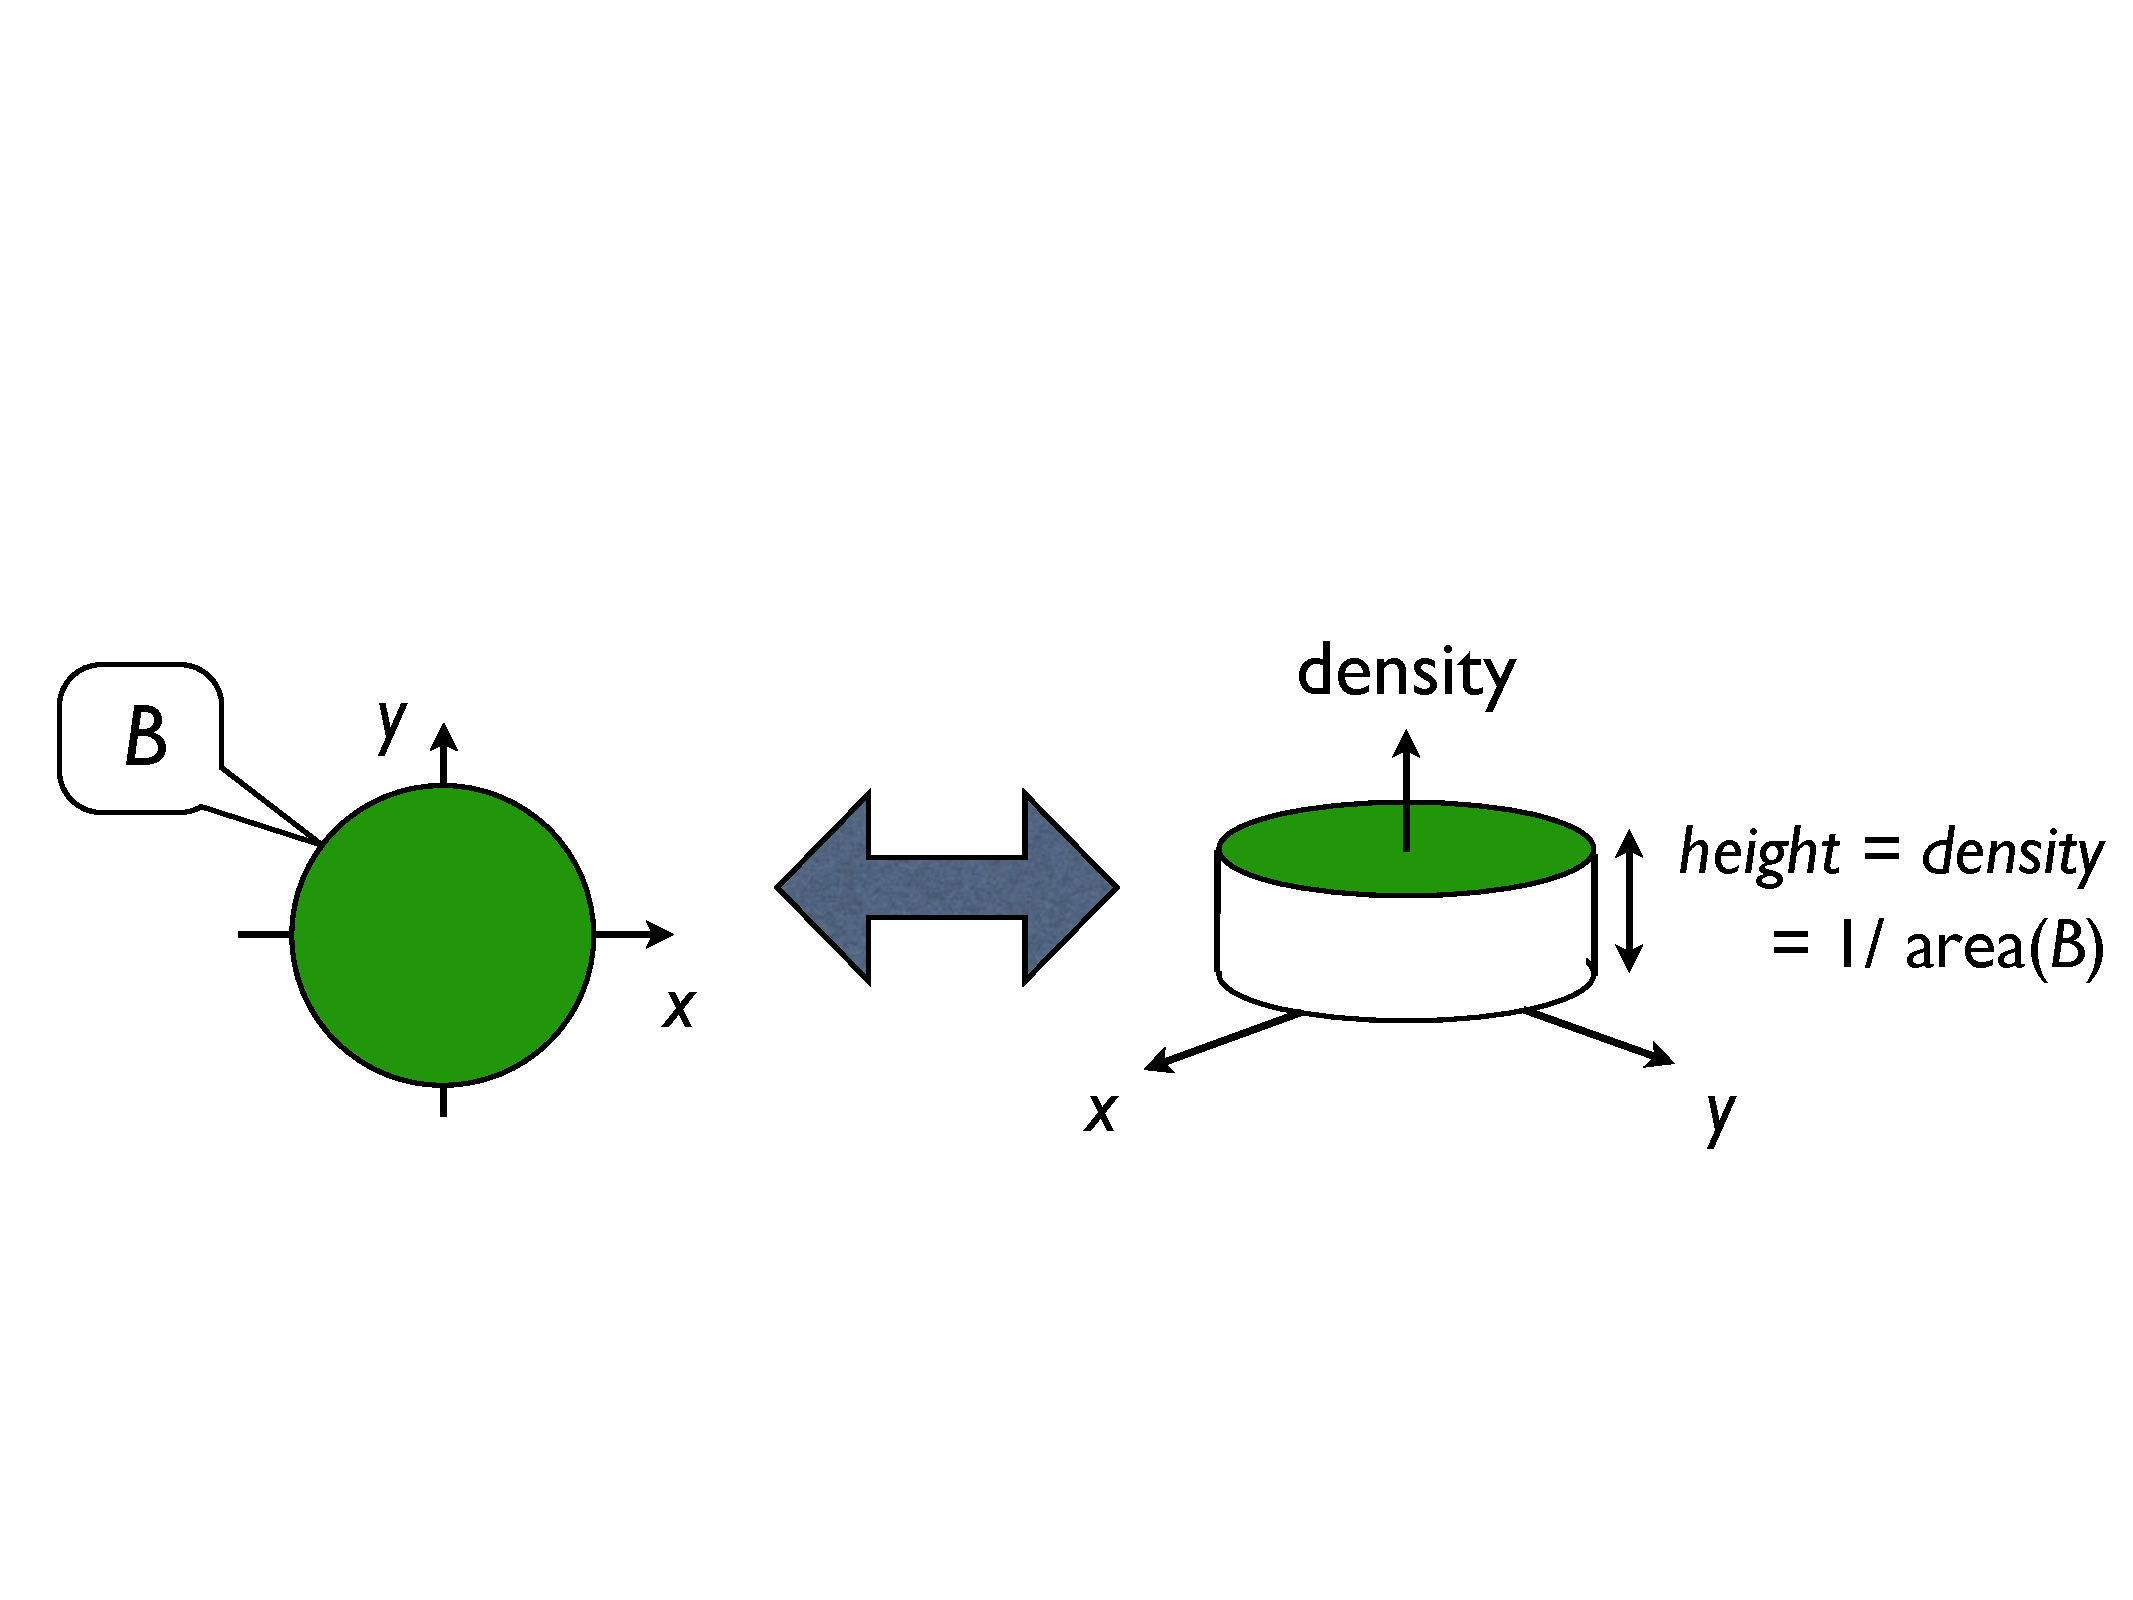
\includegraphics[width=0.7\linewidth]{figures/uniform-on-circle}
\end{center}

\begin{enumerate}
  \item Find $\E[XY], \E[X], \E[Y]$. Hint: use symmetry.
  \item Find $g_i$'s such that $\E[g_1(X) g_2(Y)] = 0$ but $\E[g_1(X)] \E[g_2(Y)] > 0$. Hint: use the indicators shown in the figure below.
\end{enumerate}
\begin{center}
	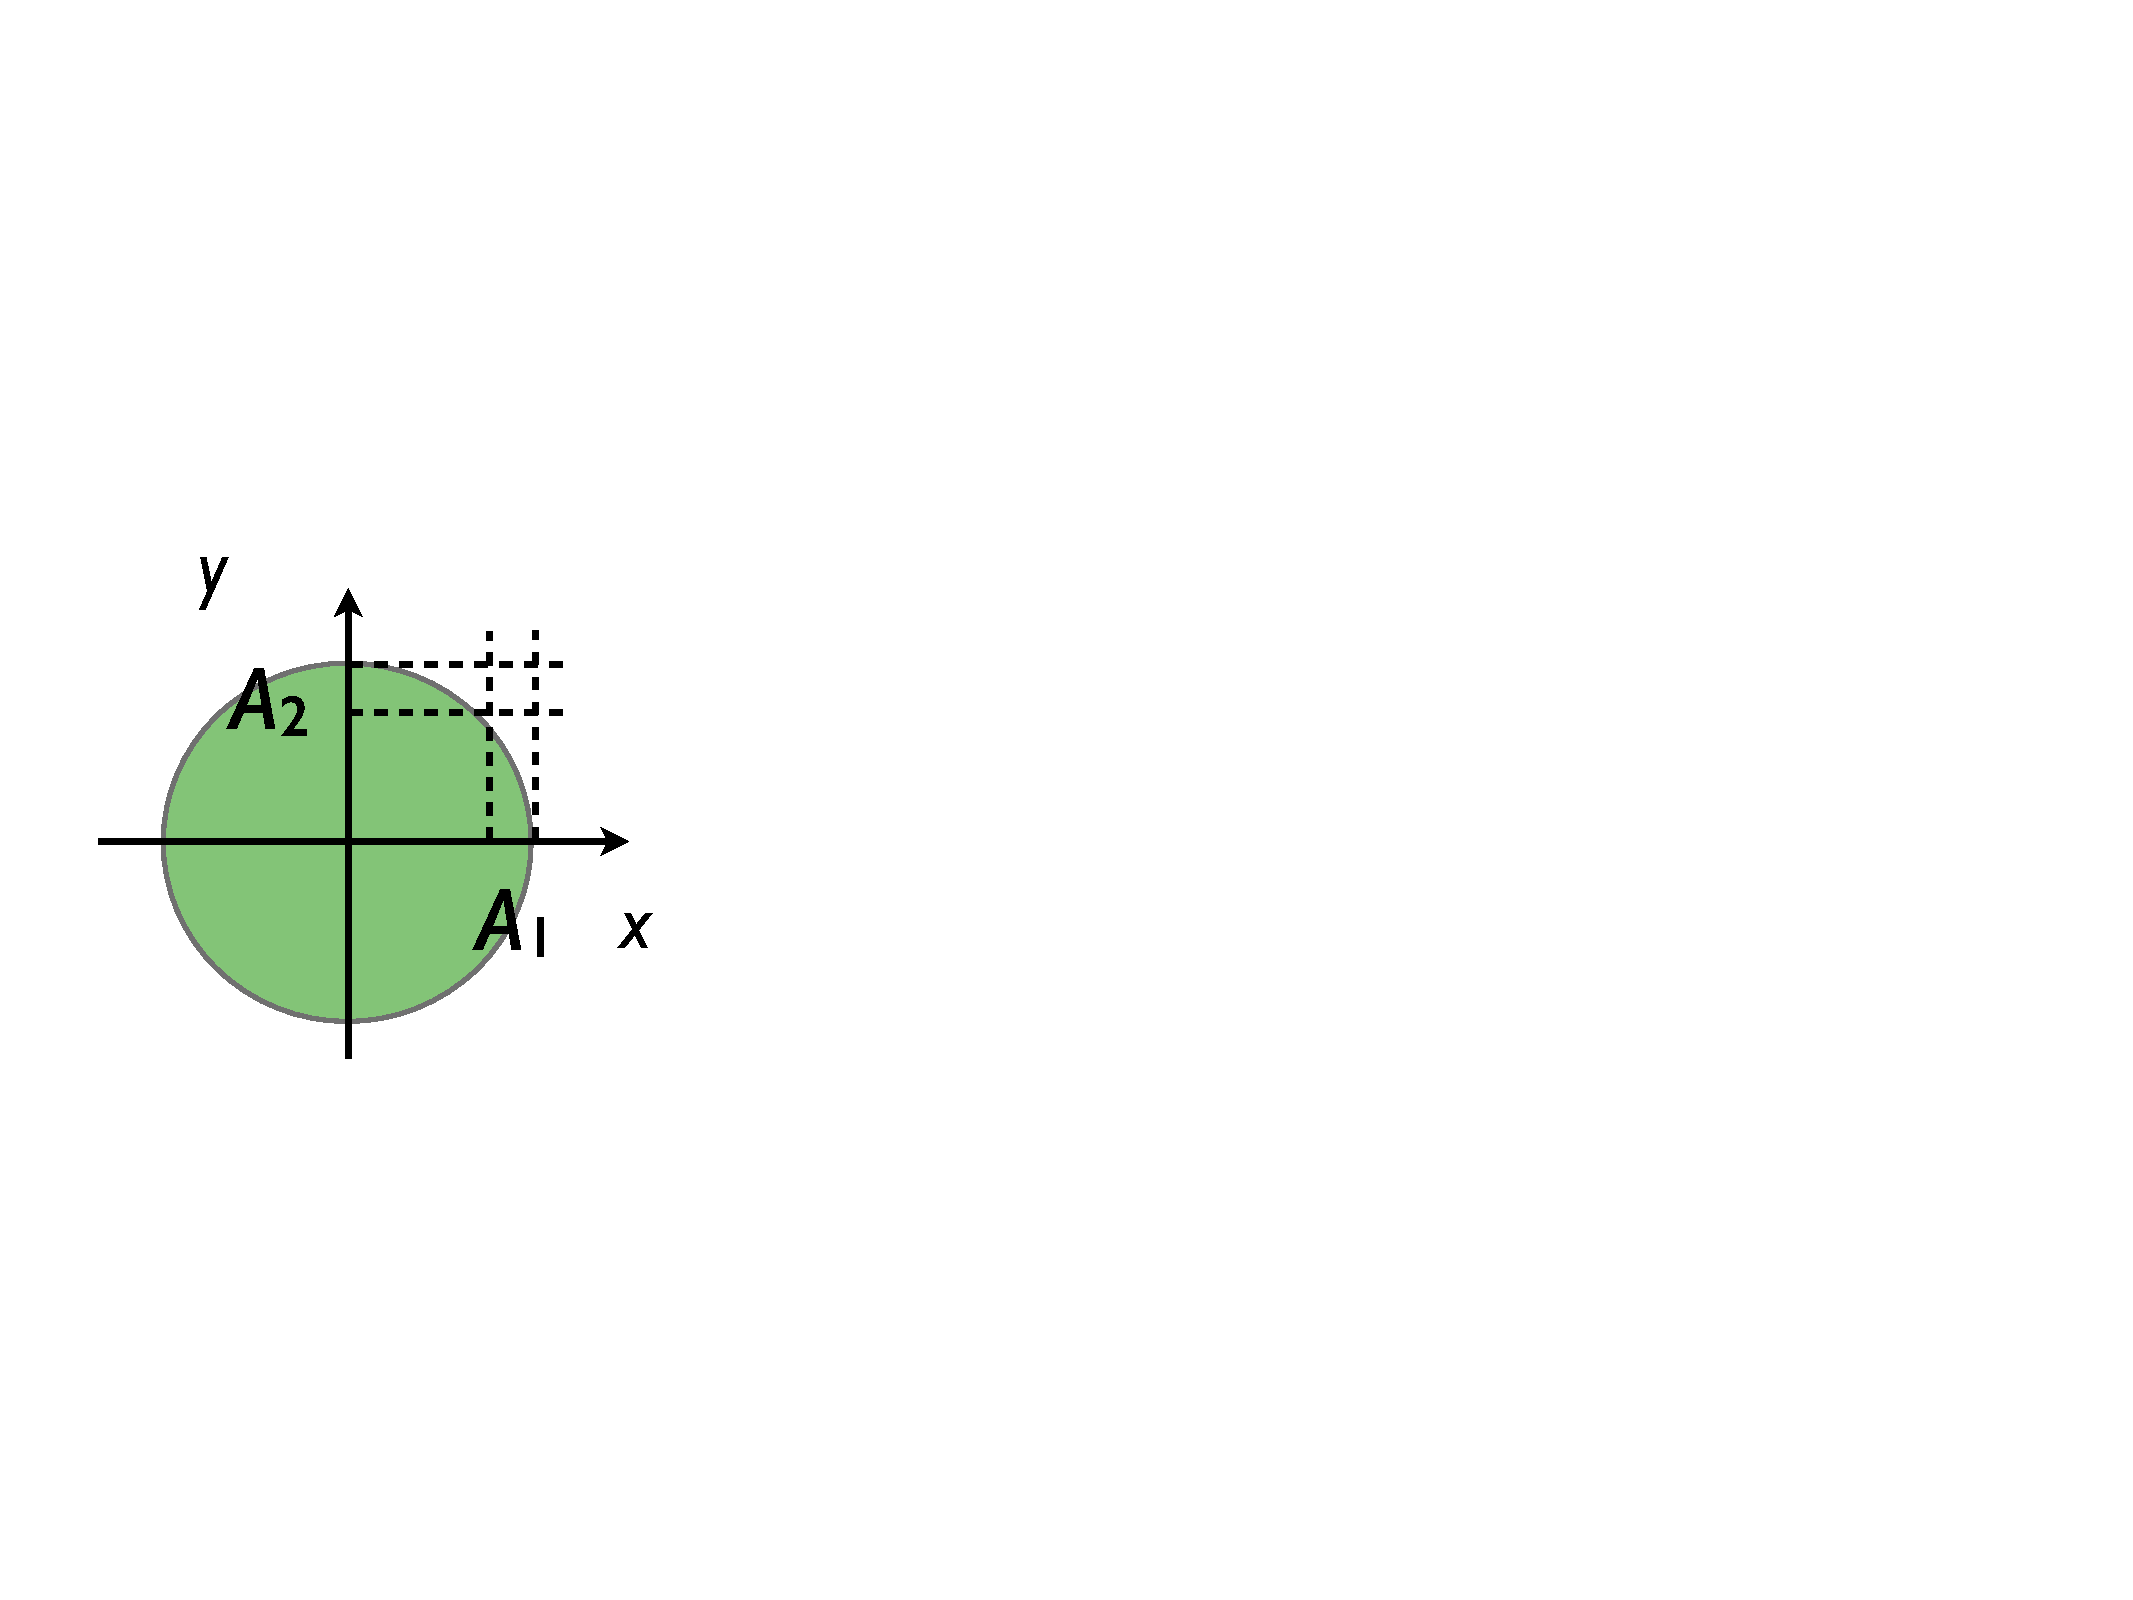
\includegraphics[width=0.2\linewidth]{figures/circle-indicators}
\end{center}


\subsection{Declaring independent random variables}

Let us continue the discussion of Section~\ref{sec:using-rv-to-construct-prs}, on implicit specification of probability spaces. Suppose now we want to declare more than one random variables. Often we do so by declaring that (1) they are independent, and (2) the distribution of each random variable. For example: ``let $X_1, X_2, \dots$ be independent $\Bern(0.5)$ random variables.'' A shorthand: ``$X_1, X_2, \dots$ are i.i.d. $\Bern(0.5)$'' (identically and independently distributed). Or just:
\[ X_i \iidsim \Bern(p). \]

\point{There is always some $\Omega$, $\P$, $\events$, $X_1$, $X_2$, \dots satisfying the constraints (1) and (2):} you can take this as a fact (search Kolmogorov's Extension Theorem if you are curious). 

\point{This does not uniquely specify $\Omega$, $\P$, $\events$, $X_1$, $X_2$, \dots:} for the same reason as in Section~\ref{sec:using-rv-to-construct-prs}.

\point{But:} in the light of Section~\ref{sec:expectation-indep}, all we need to know to compute expectation is (1) to know that the random variables are independent and (2) the distribution of each random variable $X_i$ (called the ``marginal distributions'').


\subsection{Computing expectation using the cumulative distribution function}

\point{Idea:} consider the following identity, which holds true for all $x \ge 0$, 
\[ x = \int_0^\infty \1[x > t] \ud t. \]
Now for $X \ge 0$, let us take expectations on both sides and use Fubini:
\[ \E X = \int_\Omega X \ud \P = \int_\Omega \int_0^\infty \1[X > t] \ud t \ud \P =  \int_0^\infty \int_\Omega \1[X > t] \ud \P  \ud t, \]
which yields:
\[ \E X = \int_0^\infty \P[X > t] \ud t = \int_0^\infty (1 - F_X(t))  \ud t. \]


\subsection{Transformations of random variables and random vectors}

\point{One dimension.} In light of exercise~6 in Section~\ref{sec:ex-set-2}, it should not be a surprise how to solve the following problem: ``given a random variable $X$ with known density $f_X$ (with respect to the Lebesgue measure), and strictly increasing, differentiable function $g$, find the density of $Y=g(X)$ (again, with respect to the Lebesgue measure).''

\point{Solution:} from exercise~6 in Section~\ref{sec:ex-set-2}, we already know the CDF $F_Y$ of $Y$, namely $F_Y(y) = F_X(g^{-1}(y))$. To get the density $f_Y$ of $Y$, based on Section~\ref{sec:calculus}, we simply take the derivative with respect to $y$ and use chain rule, obtaining:
\[ f_Y(y) = \frac{\ud}{\ud y} F_X(g^{-1}(y)) = f_X(g^{-1}(y)) \frac{\ud}{\ud y} g^{-1}(y). \]

\point{The multivariate version} is a natural extension of the above formula: let $X : \Omega \to \R^n$ denote a random vector with density $f_X : \R^n \to [0, \infty)$, let $g : \R^n \to \R^n$ be invertible with both $g$ and $g^{-1}$ continuously differentiable (a so called $C_1$ \emph{diffeomorphism}), then the density of $f_Y : \R^n \to [0, \infty)$ is given by
\[ f_Y(y) = f_X(g^{-1}(y)) \left| \det \left( \frac{\partial}{\partial y_c} g_r^{-1}(y) \right) \right| \]
where the derivative is generalized into the determinant of a Jacobian matrix indexed by rows $r \in \{1, 2, \dots, n\}$ and columns $c \in \{1, 2, \dots, n\}$. 

\point{Note:} the above theorem can be modified to change $\R^n$ to open subsets of $\R^n$ in the obvious way, which is useful when $X$ takes values in a subset of $\R^n$ such as the \emph{simplex} (a list of $n$ positive numbers that sum to one) in the case of a Dirichlet random variable. 

\point{For computations:} it is often easier to compute the derivative of $g$ rather than $g^{-1}$, and thankfully using properties of Jacobian matrices,
\[  \left| \det \left( \frac{\partial}{\partial y_c} g_r^{-1}(y) \right) \right| = \frac{1}{\left| \det \left( \frac{\partial}{\partial y_c} g_r(y) \right) \right|}. \]

\point{Example:} if $X_1 \sim \text{Exp}(1)$ and $X_2 \sim \text{Exp}(1)$ are independent, show that $Y = X_1 / (X_1 + X_2)$ is uniform between zero and one.  Hint: the function $g(x_1, x_2) = x_1 / (x_1 + x_2)$ is not a diffeomorphism (it looses information) so you cannot apply the above theorem directly! Use instead $g(x_1, x_2) = (x_1 / (x_1 + x_2), x_1 + x_2)$. This augmentation trick is often useful. In computational statistics it forms the basis of ``reversible jump Markov chain Monte Carlo,'' a method used in Bayesian statistics to select among models of different dimensionalities which fits better the data.

\point{Do you really need to do this?} Not always! Sometimes you may be only interested in the expectation of the transformed random variable $\E[Y]$. In this case, we know from the first assignment that this can be done directly without computing $g^{-1}$ or derivatives via:
\[ \E[Y] = \int g(x) f_X(x) \ud x. \]
This is often much quicker than finding $f_Y$ and then computing
\[ \E[Y] = \int y f_Y(y) \ud y. \]
However in other cases, such as when a random variable is not well summarized by its first few moments (e.g. mean and variance), you will have to compute $f_Y$.


\section{Asymptotics}

Often we are faced with a question about a large number of random variables, say $X_1, X_2, \dots, X_{1,000,000,000}$. In the context of big data, or big models, or large Monte Carlo simulations, the number of random variables of interest can be quite large. Providing an exact answer to questions involving so many random variables is often  computationally prohibitive or impossible. 

\point{Key observation:} paradoxically, under certain angles, the behaviour of large sets of random variables becomes increasingly simple. This allows us to make approximations. Asymptotics is the field concerned with making sure that these approximations can become arbitrarily accurate as the number of random variables increases. Moreover, asymptotics can sometimes give some hint on how to compare different approximations, i.e. how fast approximations converge (\emph{rates}). 


\subsection{Infinitely often and eventually}\label{sec:io-ev}

\point{Motivation:} Let $X_1, X_2, X_3, \dots$ be iid non-atomic (continuous) random variables representing the best performance achieved in a sport (e.g. 100m freestyle) at consecutive olympic games. Let $R_n$ denote the indicator variable that a record is broken at olympic $n$ (i.e. $R_n = 1$ if $X_n > X_j$ for all $j = 1, 2, \dots, n-1$, and $R_n = 0$ otherwise). Let $A_n = (R_n = 1)$. What is the probability that records are broken infinitely often? One! Let $B_n = (R_n R_{n+1} = 1)$. What is the probability that records are broken in two consecutive years infinitely often? Zero! Why? And how to define ``infinitely often'' formally?

\point{Definition:} Let $A_n$ denote an infinite collection of events, $n\in\{1,2,3,\dots\}$ (not necessarily nested). We create two new events from these:
\begin{eqnarray*}
(A_n\ev) &\defeq& \{\omega \in \Omega : \exists N \in \{1, 2, \dots\}, \forall n\ge N, \omega \in A_n \} \\
(A_n\io) &\defeq& \{\omega \in \Omega : \forall N \in \{1, 2, \dots\}, \exists n\ge N, \omega \in A_n \}.
\end{eqnarray*}

\point{Examples:} consider the ``drunk train'' example from the first lecture.  
\begin{itemize}
  \item Let $X_i = 2Y_i - 1$ denote the direction the train takes at each step where $Y_i \sim \Bern(1/2)$ are iid (independent and identically distributed)
  \item Let $S_n = X_1 + X_2 + \dots + X_n$ denotes the current position of the train. 
  \item Let $A_n$ denote the event that the train is at ``home'' at step $n$, i.e. $A_n = (S_n = 0)$.
  \item The event that the train never gets lost: call this the event $A$, i.e. that the train returns to zero infinitely often. $A \defeq (A_n\io)$.
  \item The event that train eventually gets lost: $B \defeq (S_n \neq 0\ev)$.
\end{itemize}

\point{Proposition:} $(A_n\io) = (A_n^\complement\ev)^\complement$.

\point{Proof:} by definition:
\begin{eqnarray*}
(A_n\io) &=& \bigcap_{N=1}^\infty \bigcup_{n\ge N} A_n \\
(A_n\ev) &=& \bigcup_{N=1}^\infty \bigcap_{n\ge N} A_n.
\end{eqnarray*}
The proposition follows from De Morgan's law.


\subsection{Borel-Cantelli (BC) lemma 1}

\point{Proposition:} If \[\sum_{n=1}^\infty \P(A_n) < \infty,\] then $\P(A_n\io) = 0$.

\point{Notes:}
\begin{itemize}
  \item $A_n$ do not need to be independent/disjoint/nested!
  \item But independence will be needed for a partial converse (BC 2)
\end{itemize}

\point{Example:} A drunk bird eventually gets lost (with probability one).
\begin{itemize}
  \item Let $X_i^{(3)} \defeq (X^{(1)}_i, X'^{(1)}_i, X''^{(1)}_i)$, where the three coordiates are indendent copies of the random walk of Section~\ref{sec:io-ev}. I.e. diagonal moves are permitted.
  \item Similarly, $S_n^{(3)} = X_1^{(3)} + X_2^{(3)} + \dots + X_n^{(3)}$.
  \item The claim can be rewritten as $\P(S^{(3)}_n = (0,0,0)\io) = 0$.
  \begin{enumerate}
    \item First, by the binomial formula, \[\P(S^{(1)}_{2n} = 0) = \binom{2n}{n} 2^{-2n}.\]
    Why? Well each individual path of length $2n$ has probability $2^{-2n}$. How many such paths are at zero at step $2n$? Those where you go up $n$ times and down $n$ times. Counting the number of paths is like counting the subset of $\{1, 2, \dots, 2n\}$ where we go up. There are $\binom{2n}{n}$ subsets of $\{1, 2, \dots, 2n\}$ of size $n$.
    \item Next, apply Stirling's formula ($n! \sim \sqrt{2 \pi n}\left(\frac{n}{e}\right)^n$) to get \[\P(S^{(1)}_{2n} = 0)  \sim \frac{c}{\sqrt{n}},\] where $c$ is a constant, and $a_n \sim b_n$ means that $a_n/b_n \to 1$.
    \item This means that for the whole process,  \[\P(S^{(3)}_{2n} = 0)  \sim \frac{c}{n^{3/2}},\] which is summable, i.e. \[ \sum_{n=1}^\infty \frac{c}{n^{3/2}} < \infty,\] because $3/2 > 1$.
    \item Hence, by BC 1, $\P(S^{(3)}_n = (0,0,0)\io) = 0$.
  \end{enumerate}
\end{itemize}

\point{Proof of BC:} let $N$ denote the number of $A_n$'s that occur: \[ N = \sum_{n=1}^\infty \1_{A_n}. \]We have:
\begin{enumerate}
  \item $(N = \infty) = (A_n\io)$,
  \item By MCT: 
\begin{eqnarray*}
\E[N] &=& \E\left[\sum_{n=1}^\infty \1_{A_n}\right] \\
&=& \sum_{n=1}^\infty \P(A_n).
\end{eqnarray*} 
  \item Hence by the assumption, $\E[N] < \infty$.
  \item It follows that $\P(N = \infty) = 0$.
\end{enumerate}

\point{Converse?} It is NOT true that \[ \P(A_n\io) = 0 \Longrightarrow \sum \P(A_n) < \infty. \] Counter-example:
\begin{itemize}
	\item Let $\P$ be uniform on $[0, 1]$.
  \item Take $A_n = [0, 1/n]$.
  \item We have $(A_n \io) = \{0\}$, hence $\P(A_n \io) = 0$.
  \item But $\sum \P(A_n) = \infty$.
\end{itemize}

\point{But if we add independence, it is true:} (BC 2) If \[ \sum_{n=1}^\infty \P(A_n) = \infty,\]and the events $A_n$ are independent, then $\P(A_n\io) = 1$.

\point{Example:} a monkey on a typewriter will write the complete work of Shakespeare infinitely often. Some notation first:
\begin{itemize}
  \item Denote the work of Shakespeare by $x_0, x_1, x_2, \dots, x_{k-1}$ where each $x_i$ is a letter.
  \item Let $M_i$ denote the letter pressed by the monkey at step $i$. Assume the $\{M_i\}$ are independent.
  \item Define $A_n \defeq (M_n = x_0, M_{n+1} = x_1, \dots, M_{n+k-1} = x_{k-1})$.
\end{itemize}
Problem? $A_n$ are not independent! We will actually prove something stronger. Informally, the idea is that we are going to show the monkey write the work of Shakespeare \emph{and with the first letter written say Jan 1st} infinitely often. Formally:
\begin{itemize}
  \item Define $A'_n \defeq (M_{kn} = x_0, M_{kn+1} = x_1, \dots, M_{kn+k-1} = x_{k-1}).$
  \item The $A'_n$ are independent by construction.
  \item Hence, by BC 2, $\P(A'_n \io) = 1$.
  \item Now, $(A'_n\io) \subset (A_n \io)$, so $\P(A_n \io) \ge \P(A'_n\io) = 1$.
\end{itemize} 


\subsection{Weak law of large number (WLLN)}

Let $X_i : \Omega \to \R$ be iid, with $\E[X_i] = \mu, |\mu| < \infty$, and defined $S_n = X_1 + \dots + X_n$. To capture our intuition of how repeated random processes behave (``frequencies approach probabilities''), we would like to be able to write something like: \[ \frac{1}{n} S_n \to \mu. \]That raises the question: what do we mean by ``$\to$''? So far, the definition we used was \emph{pointwise limits}, meaning that for all $\omega\in\Omega$, \[ \lim_{n\to\infty} \frac{1}{n} S_n(\omega) = \mu.\]Note here that the LHS is a random variable, so the right hand side should be interpreted as a constant random variable (i.e. such that $\mu(\omega) = \mu$ for all $\omega)$. 

\point{It is too much to ask} for such convergence to hold in general. Consider for instance the train example, where $\omega$ corresponds to an infinite trajectory. Then for the trajectory $\omega_0$ where the train always goes right (s.t. $X_i(\omega_0) = +1$ for all $i$). Then \[ \lim \frac{1}{n} S_n(\omega_0) = 1 \neq \mu = 0.\]

\point{Instead:} we will relax the notion of convergence. There are several ways to do this, which are useful in different contexts. Let us start with one that gives us a simple proof of the LLN.

\point{Proposition:} let $X_i : \Omega \to \R$ be iid, with $\E[X_i] = \mu, |\mu| < \infty$, and defined $S_n = X_1 + \dots + X_n$. Then for all $\epsilon > 0$, \[ \lim_{n\to\infty} \P\left( \left| \frac{1}{n} S_n - \mu\right| \ge \epsilon \right) = 0. \]

\point{Visualization:} suppose $\mu = 0$, and note that $\left( \left| \frac{1}{n} S_n -0\right| \ge \epsilon \right) = ( |S_n| > \epsilon n)$. On a graph where the x-axis is $n$ and the y-axis is $S_n$ (the same picture we used for train trajectories), consider the cone specified by $\epsilon n$ and $-\epsilon n$. The event $( |S_n| > \epsilon n)$ can be understood as selecting the trajectories that are outside the cone at step $n$. The probabilities of these events should go to zero as $n\to\infty$.
\begin{center}
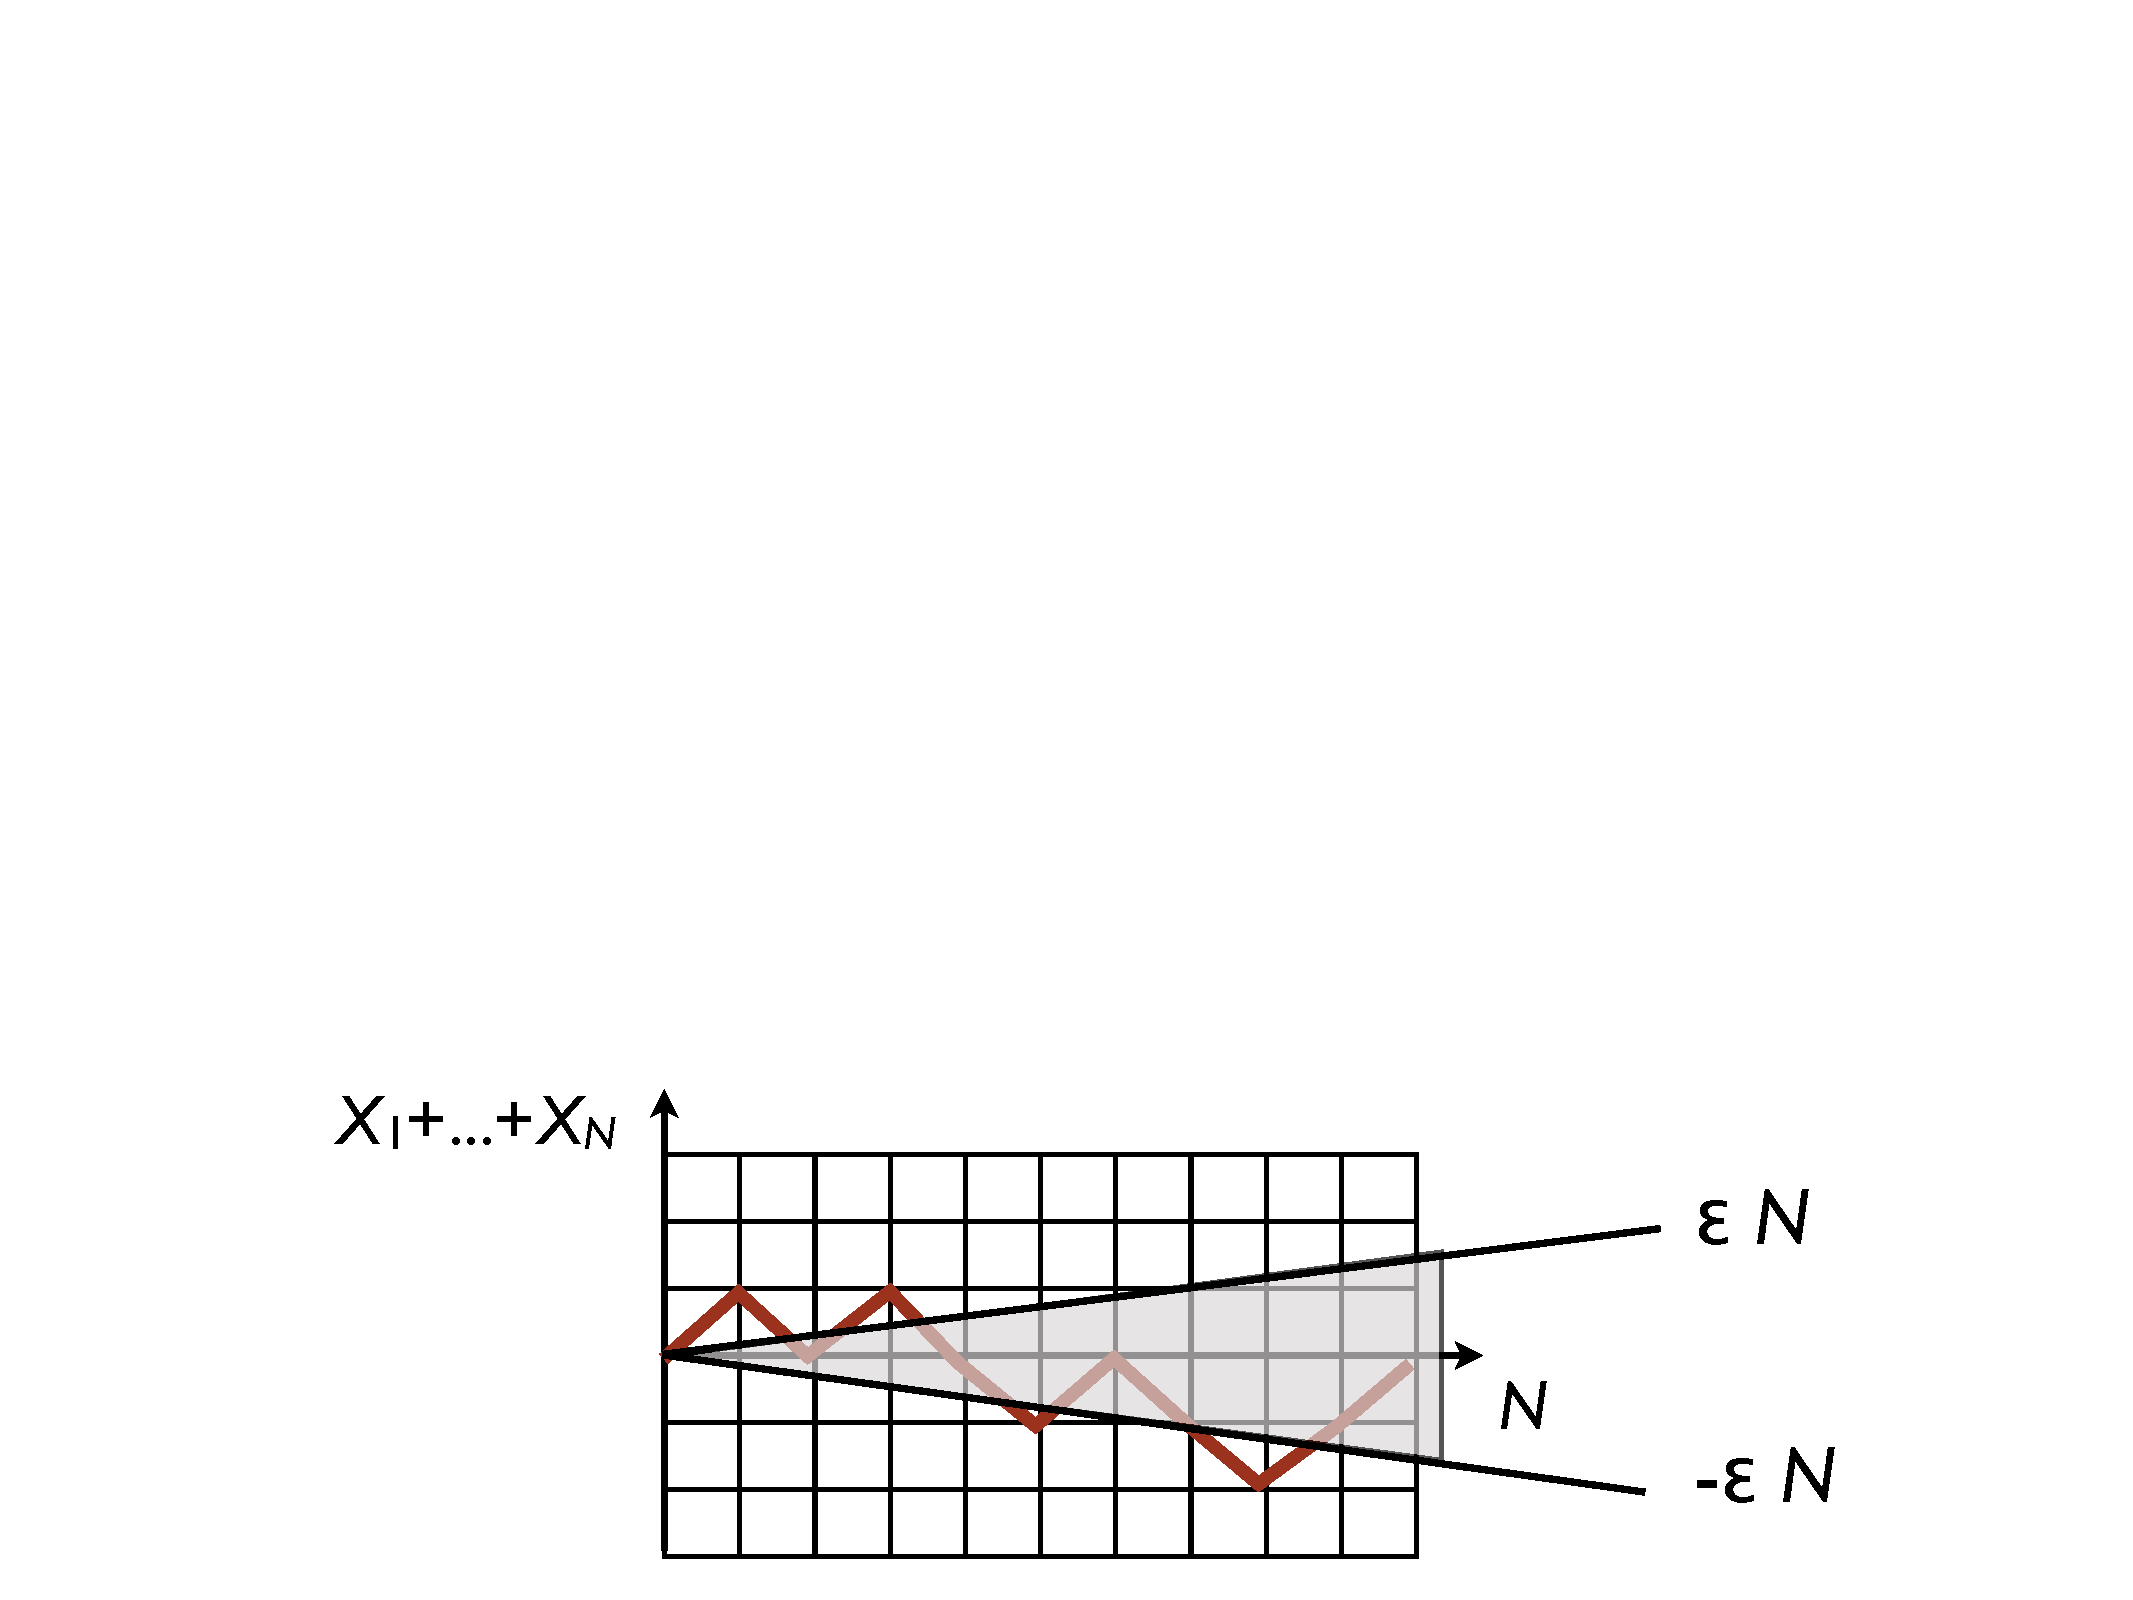
\includegraphics[width=0.7\linewidth]{figures/LLN}
\end{center}

\point{Proof:} we will start with a proof that uses an extra assumption, $\var X < \infty$. I will then give a sketch of how to get rid of this condition.
\begin{enumerate}
  \item First, assume without loss of generality that $\mu = 0$ (otherwise, set $X'_i = X_i - \mu$). 
  \item Use Chebyshev:
  \begin{eqnarray*}
    \P\left(\left|\frac{1}{n}S_n\right| \ge \epsilon \right) &\le& \frac{\E\left| \frac{1}{n} S_n \right|^2}{\epsilon^2} \\
    &=& \frac{\E[X_1 + \dots + X_n]^2}{n^2 \epsilon^2} \\
    &=& \frac{\sum_{i=1}^n \E[X_i^2] + \sum_{(i,j):i\neq j} \E[X_i X_j]}{n^2 \epsilon^2} \\
    &=& \frac{n \E X_i^2}{n^2 \epsilon^2} \\
    &=& \frac{\text{constant}}{n}.
  \end{eqnarray*}
  \item Taking limits on both sides: \[ \lim_{n\to\infty} \P\left(\left|\frac{1}{n}S_n\right| \ge \epsilon \right) \le \lim_{n\to\infty} \frac{\text{constant}}{n} = 0. \]
\end{enumerate}

\point{Note:} we actually only used pairwise uncorrelation in this proof.

\point{Sketch:} for how to lift the finite variance condition. The idea is to first fix $x > 0$, and to write the following decomposition:
\[ X_i = \underbrace{X_i \1[|X_i| \le x]}_{Y_i} + \underbrace{X_i \1[|X_i| > x]}_{Z_i}. \]
Now we can use our previous result on $Y_i$ since a bounded random variable will necessarily have finite variance. As for $Z_i$, we can get rid of it by letting $x \to \infty$ and using DCT (where we use $|Z_i| \le |X_i|$ and our assumption that $|\mu| < \infty$ and hence $\E|X_i| < \infty$).


\subsection{Convergence in probability}

The definition of ``$\to$'' used in the previous section is used in other contexts, so let us give a name to it:

\point{Definition:} a sequence of random variables $Y_i : \Omega \to \R$ converges in probability to a random variable $Y: \Omega \to \R$ if, for all $\epsilon > 0$,
\[ \lim_{n\to\infty} \P(|Y_n - Y| > \epsilon) = 0. \]

\point{Notation:} $Y_n \pcv Y$.


\subsection{Convergence almost surely}

\point{Question:} can we come up with other notions of convergence? Yes, we will see many alternative, starting with ``almost sure'' convergence (``$Y_n \ascv Y$''). Why is this useful? With almost sure convergence, it is harder to prove the LLN, but once this is done, it is easier to establish corrolaries, e.g. that $Y_n \ascv Y$ and $Y'_n \ascv Y'$ implies $Y_n + Y'_n \ascv Y + Y'$.

\point{Definition:} a sequence of random variables $Y_i : \Omega \to \R$ converges almost surely (a.s.) to a random variable $Y: \Omega \to \R$ if \[ \P(Y_n \to Y) = 1,\] where \[ (Y_n \to Y) \defeq \{ \omega \in\Omega : \lim_{n\to\infty} |Y_n(\omega) - Y(\omega)|\text{ exists and is }=0\}. \]

\point{Note:} with this last notation, another way to write convergence pointwise is $(Y_n \to Y) = \Omega$. From this, it is clear that convergence pointwise implies convergence a.s. but not vice-versa.

\point{Notation:} $Y_n \ascv Y$.

\point{Lemma} connecting this notion of convergence back to convergence in probability as well as the notions of i.o. and ev.: $X_n \ascv X$ if and only if for all $\epsilon > 0$, $\P(|X_n - X| > \epsilon\io) = 0$.

\point{Proof:} we have: \[\omega \in (X_n \to X) \Longleftrightarrow \forall \epsilon>0, \omega\in (|X_n-X| \le \epsilon \ev),\] and hence:
\begin{eqnarray*}
X_n \ascv X &\Longleftrightarrow& \forall \epsilon >0, \P(|X_n - X| \le \epsilon \ev) = 1 \\
&\Longleftrightarrow& \forall \epsilon > 0, \P(|X_n - X| > \epsilon \io) = 0.
\end{eqnarray*}

\point{Strong law of large numbers:} under the same conditions as the WLLN, this says \[ \frac{1}{n} S_n \ascv \mu. \]

\point{Proposition:} convergence in probability does not imply convergence a.s. in general.

\point{Counter-example:} moving blip. Let $\Omega = $ points on a circle, $\P$ be uniform on the circle, and $X_i$ be defined as:
\begin{eqnarray*}
X_1 &=& \1_{[0,1/2]\text{ mod }2\pi}\\
X_2 &=& \1_{[1/2,1/2+1/3]\text{ mod }2\pi}\\
X_3 &=& \1_{[1/2+1/3,1/2+1/3+1/4]\text{ mod }2\pi}\\
&\vdots&
\end{eqnarray*}
\begin{center}
	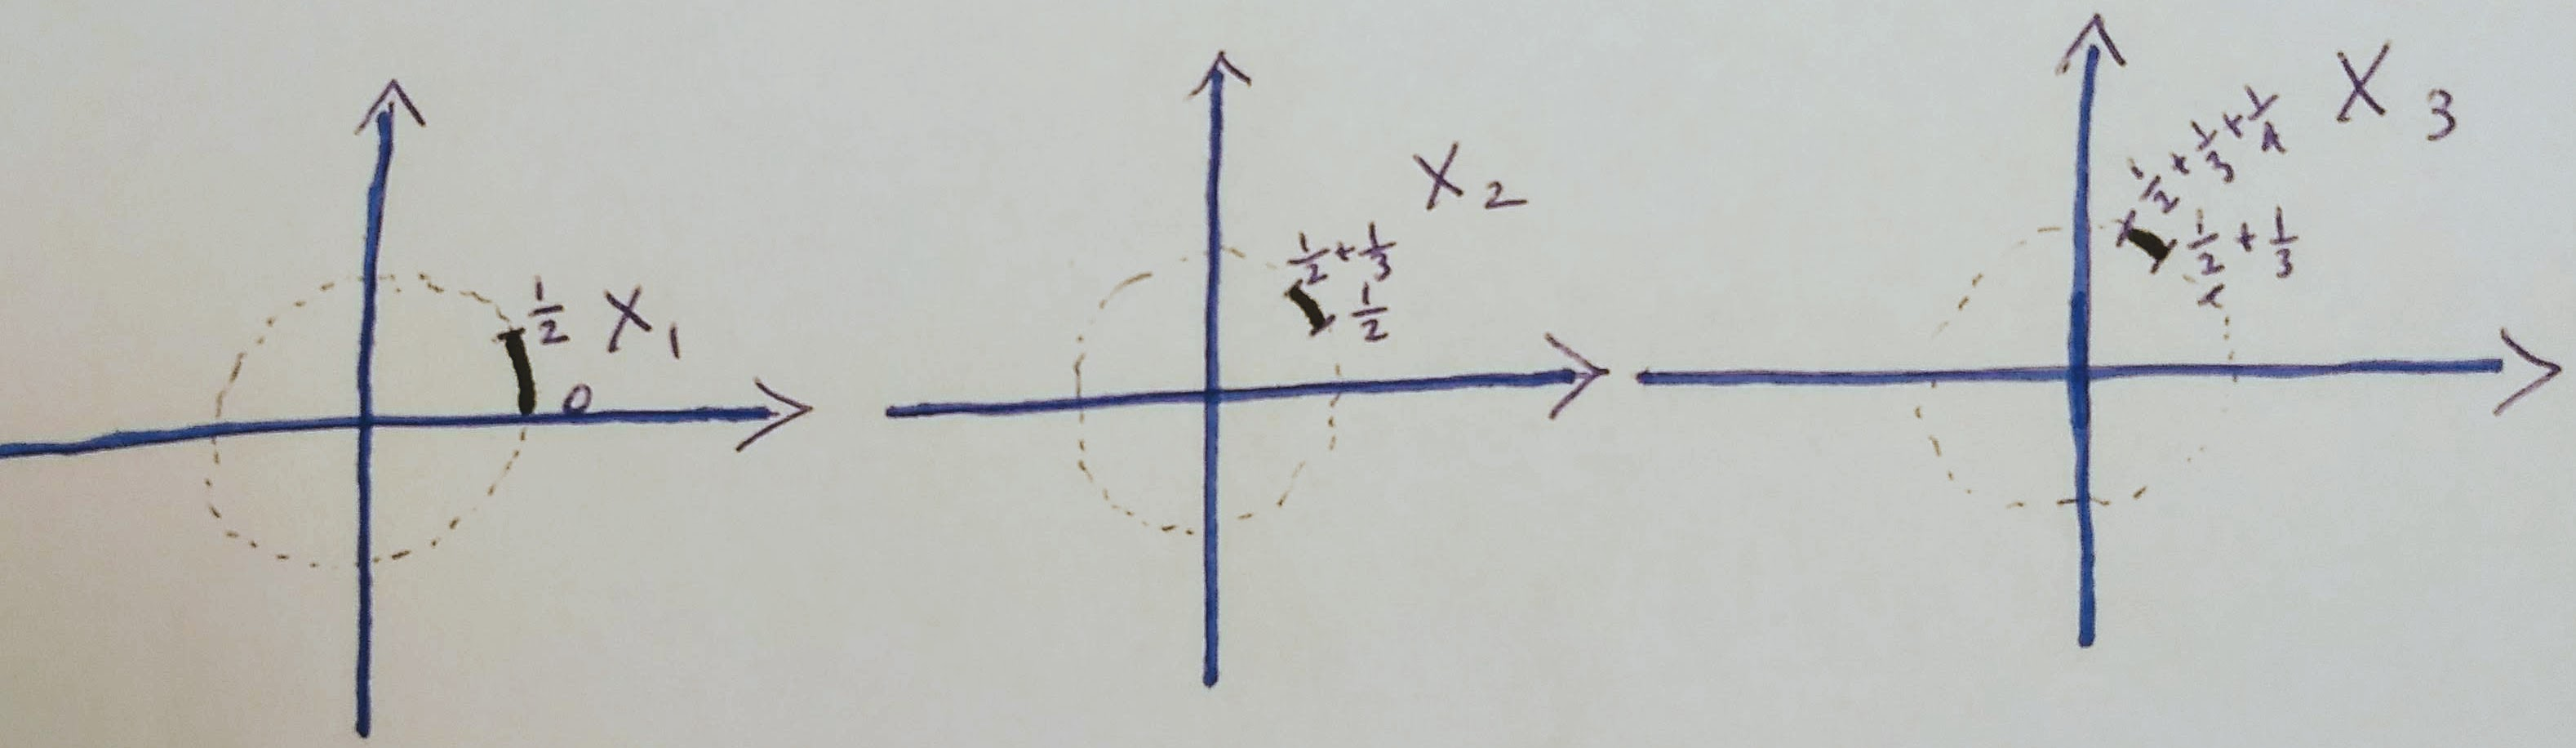
\includegraphics[width=0.8\linewidth]{figures/moving-blip} 
\end{center}

\point{Proposition:} convergence a.s. implies convergence in probability.

\point{Proof:} according to our earlier lemma, we have for all $\epsilon > 0$, $\P(|X_n - X| > \epsilon\io) = 0$. Then, if we let $A_n \defeq (|X_n - X| > \epsilon)$:
\begin{eqnarray*}
0 &=& \P\left( \bigcap_{k=1}^\infty \bigcup_{n \ge k} A_n \right) \\
&=& \lim_{k\to\infty} \P\left( \bigcup_{n\ge k} A_n \right) \text{ (by monotonicity of }\P\text{)} \\
&\ge& \lim_{k\to\infty} \P(A_k) \ge 0.
\end{eqnarray*}
It follows that $\lim_{k\to\infty} \P(A_k) = 0$.


\subsection{Toward Central Limit Theorems} 

Central limit theorems (CLT) are tools to approximate the distribution of a sum of certain random variables, $S_n = \sum_{i=1}^n X_i$. Before we describe CLTs and their proofs, let us motive the problem by first computing the exact distribution of $S_n$ to illustrate why it is non-trivial.


\subsection{Exact distribution of sums of random variables}

Let us say we have two iid random variables $X$ and $Y$ with densites $f_X$ and $f_Y$. What is the distribution of $Z = X + Y$? It is not as easy as it looks, for example you should certainly not average the densities (check! either by playing Settlers of Catan, or deriving the pmf of the sum of two dice).

\point{Example:} to make things concrete, suppose $X$ and $Y$ are iid uniform on $[0, 1]$.

\point{Compute the CDF of $Z$ first:} at a fixed point, say one, $F_Z(1)$. To do so let us use the techniques of Section \ref{sec:expectation-indep}:
\begin{align*}
\P(Z \le 1) &= \P(X + Y \le 1) \\
 &= \int \1[(x,y) \in A] f_X(x) f_Y(y) \ud x \ud y,
\end{align*}
where the region $A$ is shown in red below.
\begin{center}
	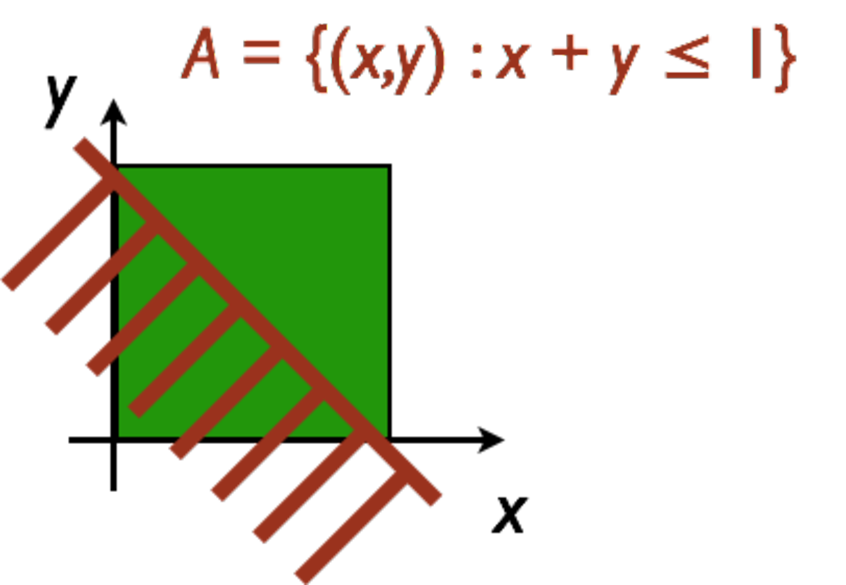
\includegraphics[width=0.3\linewidth]{figures/region} 
\end{center}
Hence 
\[ \P(Z \le 1) = \int_{-\infty}^\infty \int_{-\infty}^{1-x} f_X(x) f_Y(y) \ud y \ud x = \frac{1}{2}. \]
More generally,
\begin{align*}
\P(Z \le z) &= \int_{-\infty}^\infty \int_{-\infty}^{z-x} f_X(x) f_Y(y) \ud y \ud x \\
&= \int_{-\infty}^\infty f_X(x) \int_{-\infty}^{z-x}  f_Y(y) \ud y \ud x \\
&= \int_{-\infty}^\infty f_X(x) F_Y(z - x) \ud x
\end{align*}

\point{Computing the density:} by differentiation of the above expression with respect to the argument $z$. 
\begin{align*}
f_Z(z) &= \frac{\ud F_Z(z)}{\ud z} \\
&= \frac{\ud}{\ud z} \int_{-\infty}^\infty f_X(x) F_Y(z - x) \ud x.
\end{align*}
If only we could interchange the order of differentiation and integration that would lead to a nice expression:
\begin{align*}
f_Z(z) &=
 \int_{-\infty}^\infty f_X(x) \frac{\ud}{\ud z} F_Y(z - x) \ud x \\
  &=
  \int_{-\infty}^\infty f_X(x) f_Y(z - x) \ud x.
\end{align*}
In the next section, we justify this swap.

\point{Exercise:} show that if you sum two uniform, you get the following density, called the triangular density:
\begin{center}
	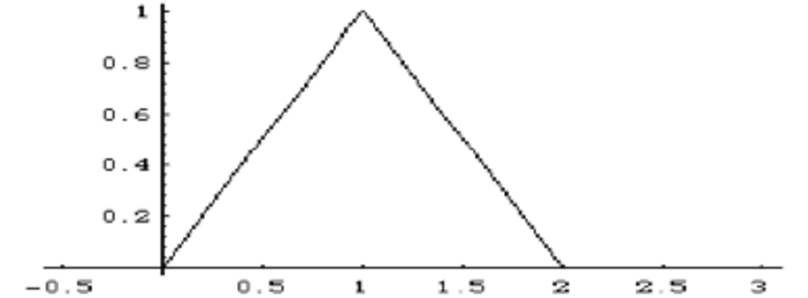
\includegraphics[width=0.3\linewidth]{figures/triangular} 
\end{center}

\point{Summing more than two variables.} In theory, generalizing this argument to more than two variables is simple, just iterate the above argument. In practice, for summing $n$ random variables we end up with a $n-1$ dimensional integral to compute. It can be tricky to compute the integral exactly, motivating the need for CLTs.\footnote{But there is one clever trick that exploit the special structure of these iterated integrals, called the Fast Fourier Transform. It uses similar techniques as the CLT. But it is still more expensive than the CLT and for sums of random vectors it can be prohibitive.}


\subsection{Interlude: exchanging the order of integration and differentiation}\label{sec:exchange}

Here we present some useful theorem justifying swapping the order of differentiation and integration. Doing so will not only justify the swap in last section, but will also be needed soon in our CLT proof. 

\point{Example: ``reparameterization trick,''} a technique very popular in machine learning. The idea is that you have a collection of probability models indexed by a parameter $\theta$ (as in Section~\ref{sec:statistical-model} for example) and you seek to compute
\[ \nabla \E_\theta [h(X)]. \] 
Here the difficulty is that the distribution of $X$ depends on $\theta$. The idea with the reparameterization trick is to remove this dependency by writing $X = g(Z, \theta)$, where the distribution of $Z$ does not depend on $\theta$. From Section~\ref{sec:inverse-cdf}, we know how to do this: set $Z$ to be uniform, and $g(\cdot, \theta)$ to the inverse CDF of $F_\theta(\cdot)$. After doing this, the hope is to swap the order of differentiation and integration:
\begin{align*}
\nabla \E_\theta [h(X)] &= \nabla \E [h(g(Z,\theta))] \;\;\text{ (always possible)} \\
&=  \E [\nabla h(g(Z,\theta))] \;\;\text{ (have to be careful here).}
\end{align*}
If we can do this, that would be nice, since we can then use the Law of large number to approximate the right hand side:
\[ \E [\nabla h(g(Z,\theta))] \approx \frac{1}{N} \sum_{n=1}^N \nabla h(g(Z^{(n)},\theta)),  \]
where $Z^{(n)}$ are iid samples, and the inner gradient is often computed using Automatic Differentiation techniques.

\point{Counter-example.} Let us see a concrete example where the above trick \emph{does not} work, to emphasize the importance of checking conditions for integral-differential swaps. Let us say $X \sim \Bern(\theta)$. We can reparametrize with $Z \sim \Unif(0,1)$ and $g(z, \theta) = \1[z < \theta]$. Indeed, $g(Z, \theta) \sim \Bern(\theta)$. We have:
\[  \frac{\ud}{\ud \theta} \underbrace{ \int_0^1 g(z, \theta) \ud z }_{=\theta} = 1,  \]
but on the other hand:
\[  \int_0^1 \underbrace{\frac{\ud}{\ud \theta} g(z, \theta)}_{=0 \text{ \emph{almost} everywhere}} \ud z = 0. \]

\point{Theorem for swaps:} suppose 
\begin{enumerate}
  \item $g(\cdot, \theta)$ is integrable for all $\theta \in [a, b]$, 
  \item $g(x, \theta)$ is differentiable for all $x$ and $\theta$, 
  \item there is an integrable envelope $h(x)$ such that $|\ud g(x, \theta) / \ud \theta| \le h(x)$ for all $x$ and $\theta$,
\end{enumerate}
then both sides of the equation below are well defined and equal:
\[ \frac{\ud}{\ud \theta} \int g(x, \theta) \mu(\ud x) = \int \frac{\ud}{\ud \theta} g(x, \theta)   \mu(\ud x). \]

\point{Exercise:} find the condition that does not hold in the counter example.

\point{Exercise:} use DCT and the mean value theorem to prove the theorem for swaps.


\subsection{CLT: numerical exploration and intuition}\label{sec:clt-numerical}

We have seen how computing the distribution of sums $S_n = X_1 + \dots + X_n$ is tedious, even for iid random variables. Now, as promised in the introduction of this chapter, the good news is that the distribution of such sums typically becomes more and more regular.

\point{Numerical example.} To start with, let us look, for 3 possible distributions for $X_i$, what the distribution of the sums look like when we increase $n$. The columns are three different distributions for $X_1$, and each row shows $S_n$ for $n \in \{1,2,4,8,16,32\}$.   
\begin{center}
	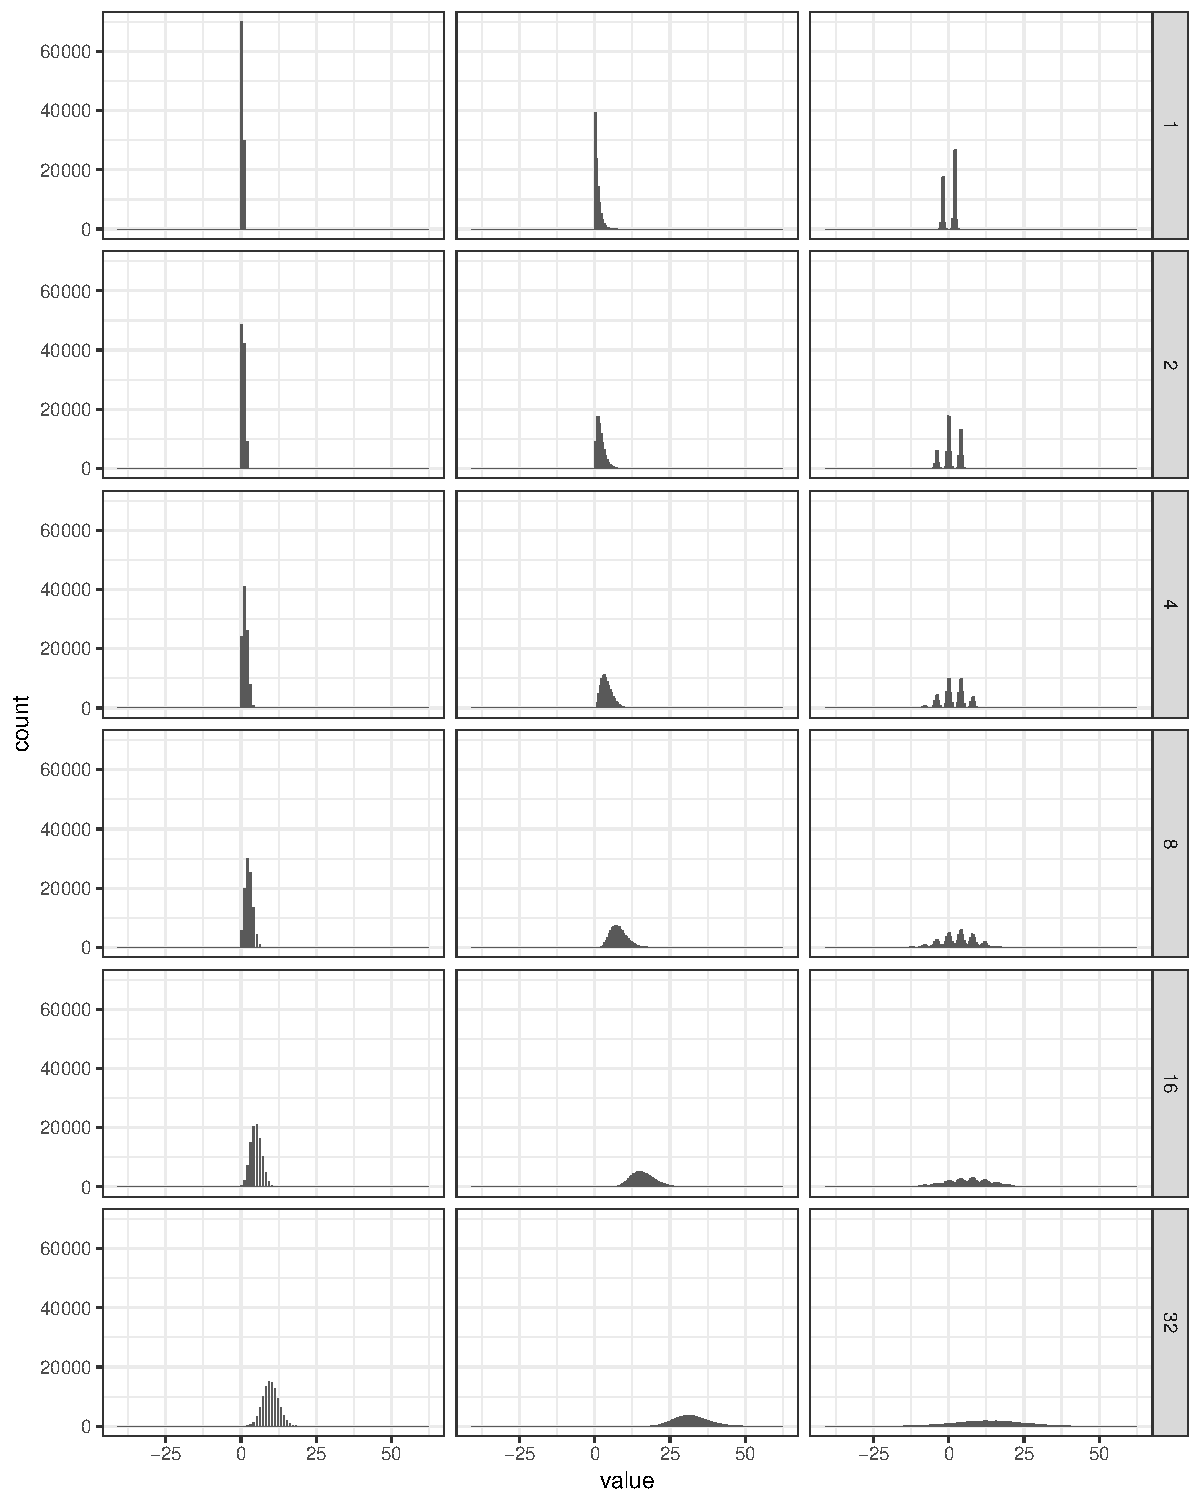
\includegraphics[width=1.0\linewidth]{figures/sums} 
\end{center}
As you can see, we start with three very different distributions (first row, $n=1$, shows the distribution of $S_1 = X_1$):
\begin{enumerate}
	\item A discrete distribution: Bernoulli distribution $X_i \sim \Bern(0.3)$.
	\item A continuous distribution with support on $[0, \infty)$: an exponential distribution, $X_i \sim \text{Exp}(1)$
	\item A multimodal distribution: with a density given by a \emph{mixture} of normal distribution $f_{X_i}(x) = 0.4 \normald(x; -2, 0.1) + 0.6 \normald(x; 2, 0.1)$ where $\normald(\cdot; \mu, \sigma^2)$ is the normal density (defined below).
\end{enumerate}

\point{Normal approximation:} notice that for $n=32$, all three look the same, up to stretching and translation. In fact, all three look like normal distributions! This is surprising, since the normal is continuous on $(-\infty, \infty)$ and unimodal, which neither of the three starting distribution $X_1$ remotely looked like! Our next big goal is to understand why!

\point{Heuristic.} Before going into proofs, however, the above numerical study already motivates the following heuristic:
\begin{enumerate}
	\item Find the mean $\mu$ and variance $\sigma^2$ of $S_n$. (why? in the ``normal approximation'' paragraph above, we say all three ``look like normal distributions,'' now we need to find which normal distribution!
	\item Let $Z_n$ denote a normal distribution with mean $\mu$ and variance $\sigma^2$, defined as the random variable with density
	\[ \normald(x; \mu, \sigma^2) = \frac{1}{\sqrt{2 \pi \sigma^2}} \exp\left(-\frac{(x-\mu)^2}{2\sigma^2}\right). \]
	\item Use the approximation $S_n \dapprox Z_n$.
\end{enumerate}

\point{Interpretation of approximation:} $S_n \dapprox Z_n$? We will need more theoretical understanding to refine what this means exactly. For now think about it as:
\begin{enumerate}
	\item $\P(S_n \le x) \approx \P(Z_n \le x)$, or
	\item $\E [ g(S_n) ] \approx \E [ g(Z_n) ]$ for nice $g$, e.g. bounded continuous.
\end{enumerate}

\point{CLTs and leaps of faith.} CLTs attempt to justify the above heuristic, either by telling us that the approximation will become arbitrarily accurate as $n \to \infty$ (basic CLT), or by providing explicit bounds on the error (Berry-Esseen theorem), or by relaxing the conditions on the random variables. In some situations, the theory might not bridge completely to your problem, but even in such cases, it might be still useful to take a ``leap of faith'' and use the normal approximation (in particular, in a situation where you might not be able to give an answer at all otherwise).

\point{Exercise:} You seed a Petri dish with a colony of 1e9 bacteria. Each day, the number of bacteria  either:
\begin{itemize}
	\item stays the same, with probability $2/5$;
	\item doubles, with probability $3/10$;
	\item quadruples, with probability $1/5$;
	\item is divided by a factor of two, with probability $1/10$.
\end{itemize}
Ten days later, what is the probability that there are more than 30e9 bacteria? 

\point{Hint:} write number of bacteria as $2^{\sum X_i}$, and rewrite the probability you want to obtain into one that can be computed using the normal approximation.


\subsection{Basic CLT}\label{sec:basic-clt}

\point{Assumptions:} the random variables we sum are independent and identically distributed and have finite variance. Also, without loss of generality assume $\E X_i = 0$ (otherwise, center the random variables).

\point{Relax:} there are CLTs for non-identical random variables, also for random vectors, and finally, for dependent random variables (e.g. certain types of Markov chains). 

\point{In relation with LLN:} sure, the LLN gives us $\frac{1}{n} S_n \ascv 0$. But this does not give us much information about how to approximate the distribution of $S_n$ for finite $n$.

\point{Exercise:} show that in fact, $\frac{1}{n^\alpha} S_n \pcv 0$ for all $\alpha > 1/2$ (the same can be done almost sure with a bit more work). 

\point{Idea:} the above exercise suggest that $\alpha = 1/2$ is a critical point. A related heuristic is that for a symmetric simple random walk, the expected distance from the origin at step $n$ is roughly $\sqrt{n}$.

\point{Theorem:} indeed, if $X_1, X_2, \dots$ are idd with $E X_1^2 = 1$ and $\E X_1 = 0$, then for any $x \in \R$:
\[ \P\left( \frac{X_1 + \dots + X_n}{\sqrt{n}} \le x\right) \to \P(Y \le x), \text{ as }n\to\infty, \]
where $Y$ is a standard normal.

\subsection{Exercise set 4}

\begin{enumerate}	
	\item First problem in Section~\ref{sec:exchange}.
	\item Second problem in Section~\ref{sec:exchange} again.
	\item One problem in Section~\ref{sec:clt-numerical}.
	\item One problem in Section~\ref{sec:basic-clt}.
\end{enumerate}


\subsection{Solutions for exercise set 4}

\point{Question 1:} there is a discontinuity at $\theta = x$, so we cannot say the function is differentiable at all points, which is required for this theorem (in contrast to many other measure theoretic ones, where almost everywhere is enough, here we really need everywhere).

\point{Question 2:} the first idea is to transform the statement into one about sequences of function in the optic of applying DCT. Let $\theta_n \to \theta$ by arbitrary in $[a,b]$. Let 
\[ h_n = \frac{g(x, \theta_n) - g(x, \theta)}{\theta_n - \theta}. \]
Note that
\[ \lim h_n = \frac{\ud g}{\ud \theta}(x, t). \]
Next let us bound $|h_n|$ by $h$:
\[ |h_n(x) | \le \sup_{\theta \in [a,b]} \left| \frac{\ud g}{\ud \theta}(x,\theta)\right| \le h(x), \] 
where we use the mean value theorem in the first inequality and the assumption on $h$ in the theorem statement for the second inequality. With this bound and the second assumption on $h$ that it is an integrable envelope, we can apply DCT and obtain the result.

\point{Question 3:} Following the hint in the question we will seek to express the number of bacteria at day 10 in terms of $2^{\sum_{i=1}^{10} X_i}$. To see this, consider the possible day-over-day changes in the number of bacteria in the Petri dish: (i) stays the same; (ii) doubles; (iii) quadruples; (iv) or is halved. Each of the changes in the number can be represented as a power of two. For example, if the number starts with value 1e9 then doubles, stays the same, quadruples, and halves in the subsequent 4 days,  the number of bacteria can be expressed succinctly as: 
\begin{align*}
\mbox{the number of bacteria after 4 days} &= 1e9 \times 2^1 \times 2^0 \times 2^2 \times 2^{-1} =
1e9 \times 2^{1 + 0 + 2 - 1} = 1e9 \times 2^{2} = 4e9. 
\end{align*}
To generalize the number of bacteria over all possible paths, we define the random variable $X_i$ to correspond to the power of 2 that the number ``grows'' in each day. Therefore, over a ten day period the (random) value of the number of bacteria is represented as $2^{\sum_{i=1}^{10} X_i}$. Since we want the number of bacteria to be more than 30 times of its initial value, we need to calculate:
\begin{align*}
\P(\mbox{more than 30e9}) &= \P\left(2^{\sum_{i=1}^{10}X_i} \geq 30\right) = \P\left(\sum_{i=1}^{10}X_i \geq \log_2(30)\right).
\end{align*}

However, we do not know the distribution of $\sum_{i=1}^{10}X_i$! Notwithstanding this limitation, this quantity is still possible to approximate. We will use the Central Limit theorem to provide an approximation which is easy to calculate. First, let $S_n := \sum^{n}_{i=0} X_i$, then:
$$S_{10} \overset{approx.}{\approx} a + bZ$$
where $Z$ follows the standard normal distribution, with:
\begin{align*}
a & = n\mu = n \cdot \E(X_i) = 10 \left( \frac{2}{5} \cdot 0 + \frac{3}{10} \cdot 1 + \frac{1}{5} \cdot 2 + \frac{1}{10} \cdot (-1) \right) = 10 \cdot 0.6 = 6 \\
b & = \sigma \sqrt{n} = \sqrt{\var(X_i) \cdot n} = \sqrt{\left( \E(X_i^2) - \E(X_i)^2 \right) \cdot 10} = \sqrt{\left( 1.2 - 0.6^2 \right) \cdot 10} = \sqrt{\frac{42}{5}}\approx 2.898,
\end{align*}
where the fact that $\E(X_i^2) = \frac{2}{5} \cdot 0^2 + \frac{3}{10} \cdot 1^2 + \frac{1}{5} \cdot 2^2 + \frac{1}{10} \cdot (-1)^2 = 1.2$ was used.

Therefore, 
\begin{align*}
\P(\mbox{more than 30e9}) &= \P\left(2^{\sum_{i=1}^{10}X_i} \geq 30\right) = \P\left(\sum_{i=1}^{10}X_i \geq \log_2(30)\right) \\ 
&= \P(S_{10} \geq \log_2{30}) = P\left(Z \geq \frac{\log_2{30} - 6}{\sqrt{\frac{42}{5}}}\right)\\&= 1 - \Phi\left(-0.3772\right) \approx 0.647.
\end{align*}

\point{Question 4:}  \begin{enumerate}
	\item First, assume without loss of generality that $\mu = 0$ (otherwise, set $X'_i = X_i - \mu$). 
	\item Use Chebyshev:
	\begin{eqnarray*}
		\P\left(\left|\frac{1}{n^\alpha}S_n\right| \ge \epsilon \right) &\le& \frac{\E\left| \frac{1}{n^\alpha} S_n \right|^2}{\epsilon^2} \\
		&=& \frac{\E[X_1 + \dots + X_n]^2}{n^{2\alpha} \epsilon^2} \\
		&=& \frac{\sum_{i=1}^n \E[X_i^2] + \sum_{(i,j):i\neq j} \E[X_i X_j]}{n^{2\alpha} \epsilon^2} \\
		&=& \frac{n \E X_i^2}{n^{2\alpha} \epsilon^2} \\
		&=& \frac{\text{constant}}{n^{2\alpha - 1}}.
	\end{eqnarray*}
	\item Taking limits on both sides: \[ \lim_{n\to\infty} \P\left(\left|\frac{1}{n^\alpha}S_n\right| \ge \epsilon \right) \le \lim_{n\to\infty} \frac{\text{constant}}{n^{2\alpha - 1}} = 0. \]
	provided $2\alpha - 1 > 0$, i.e. $\alpha > 1/2$.
\end{enumerate}
%To prove the version almost sure, we make use of a result in the posted readings:
%namely the basic $\L^2$ convergence theorem (see e.g. Du (8.3) in ch. 1) and
%of Kronecker's lemma (Du (8.5) in ch. 1). Let $X' := \frac{X}{n^\alpha}$ and
%note that
%\begin{align*}
%\sum_{i=1}^{\infty} \E {X'}_i^2 = \sum_{i=1}^{\infty} \frac{1}{n^{2\alpha}} <
%\infty 
%\end{align*}
%because $2 \alpha > 1$. We can therefore apply the basic $\L^2$ convergence
%theorem and obtain that $\sum_{i=1}^{\infty} \E X'$ converges a.s..  Kronecker's
%lemma then yields the required result.

% TODO https://en.wikipedia.org/wiki/Kolmogorov%27s_two-series_theorem
% TODO https://en.wikipedia.org/wiki/Kolmogorov%27s_inequality


\subsection{Types of convergence: big picture}\label{sec:conv-types-big-picture}

We would like to generalize the notion of convergence used in the CLT. We would like this new notion of convergence, called convergence in distribution, to sit nicely in our hierarchy of convergence modes as follows. 

\point{Covered so far:} 
\[ X_n \to X \Longrightarrow X_n \ascv X \Longrightarrow X_n \pcv X. \]

\point{Next:}
\[ X_n \pcv X \Longrightarrow X_n \dcv X. \]


\subsection{Weak convergence}

\point{Motivation:} so far, the two types of convergence we have covered assume that all random variables and the limit live in the same space: $X_i : \Omega \to \R$, $X : \Omega \to \R$. This could create problem when we formalize the central limit theorem. Why?

\point{Solution:} define convergence with respect to objects that get rid of $\Omega$ while characterizing the distribution of the random variables.

\point{Definition 1:} we say $X_n : \Omega_n \to \R$ converges in distribution to $X : \Omega \to \R$, denoted $X_n \dcv X$, if for all bounded continuous function $g : \R \to \R$ (called ``test function''), we have 
\[ \lim_{n\to\infty} \int g \ud \P_{X_n} = \int g \ud \P_X. \]

\point{Note:} more generally, weak convergence is really about convergence of measures. Similarly to the above definition, the notation $\mu_n \dcv \mu$ means that for all bounded continuous function $g$, \[ \lim_{n\to\infty} \int g \ud \mu_n = \int g \mu. \]

\point{Definition 2:} we say $X_n : \Omega_n \to \R$ converges in distribution to $X : \Omega \to \R$, denoted $X_n \dcv X$, if for all $x$ with $\P(X=x) = 0$, $F_{X_n}(x) \to F(x)$. In other words, convergence of the CDFs at points that are not atoms under $X$.

\point{Proposition (Portmanteau):} definition 1 and 2 are in fact equivalent. In fact, search Portmanteau in your favourite reference, there are many more equivalent definitions, e.g. a useful variant is to replace ``bounded continuous'' by ``Lipschitz'' (i.e. such that there is a constant $K > 0$ such that $|g(x_1) - g(x_2)| \le K |x_1 - x_2 |$.

\point{Intuition} regarding why we do not require convergence of the CDF at atomic points: otherwise, our nice hierarchy in Section~\ref{sec:conv-types-big-picture} would not hold! Consider: $X_n = 1/n$. Show it converge in probability to zero:
\begin{center}
	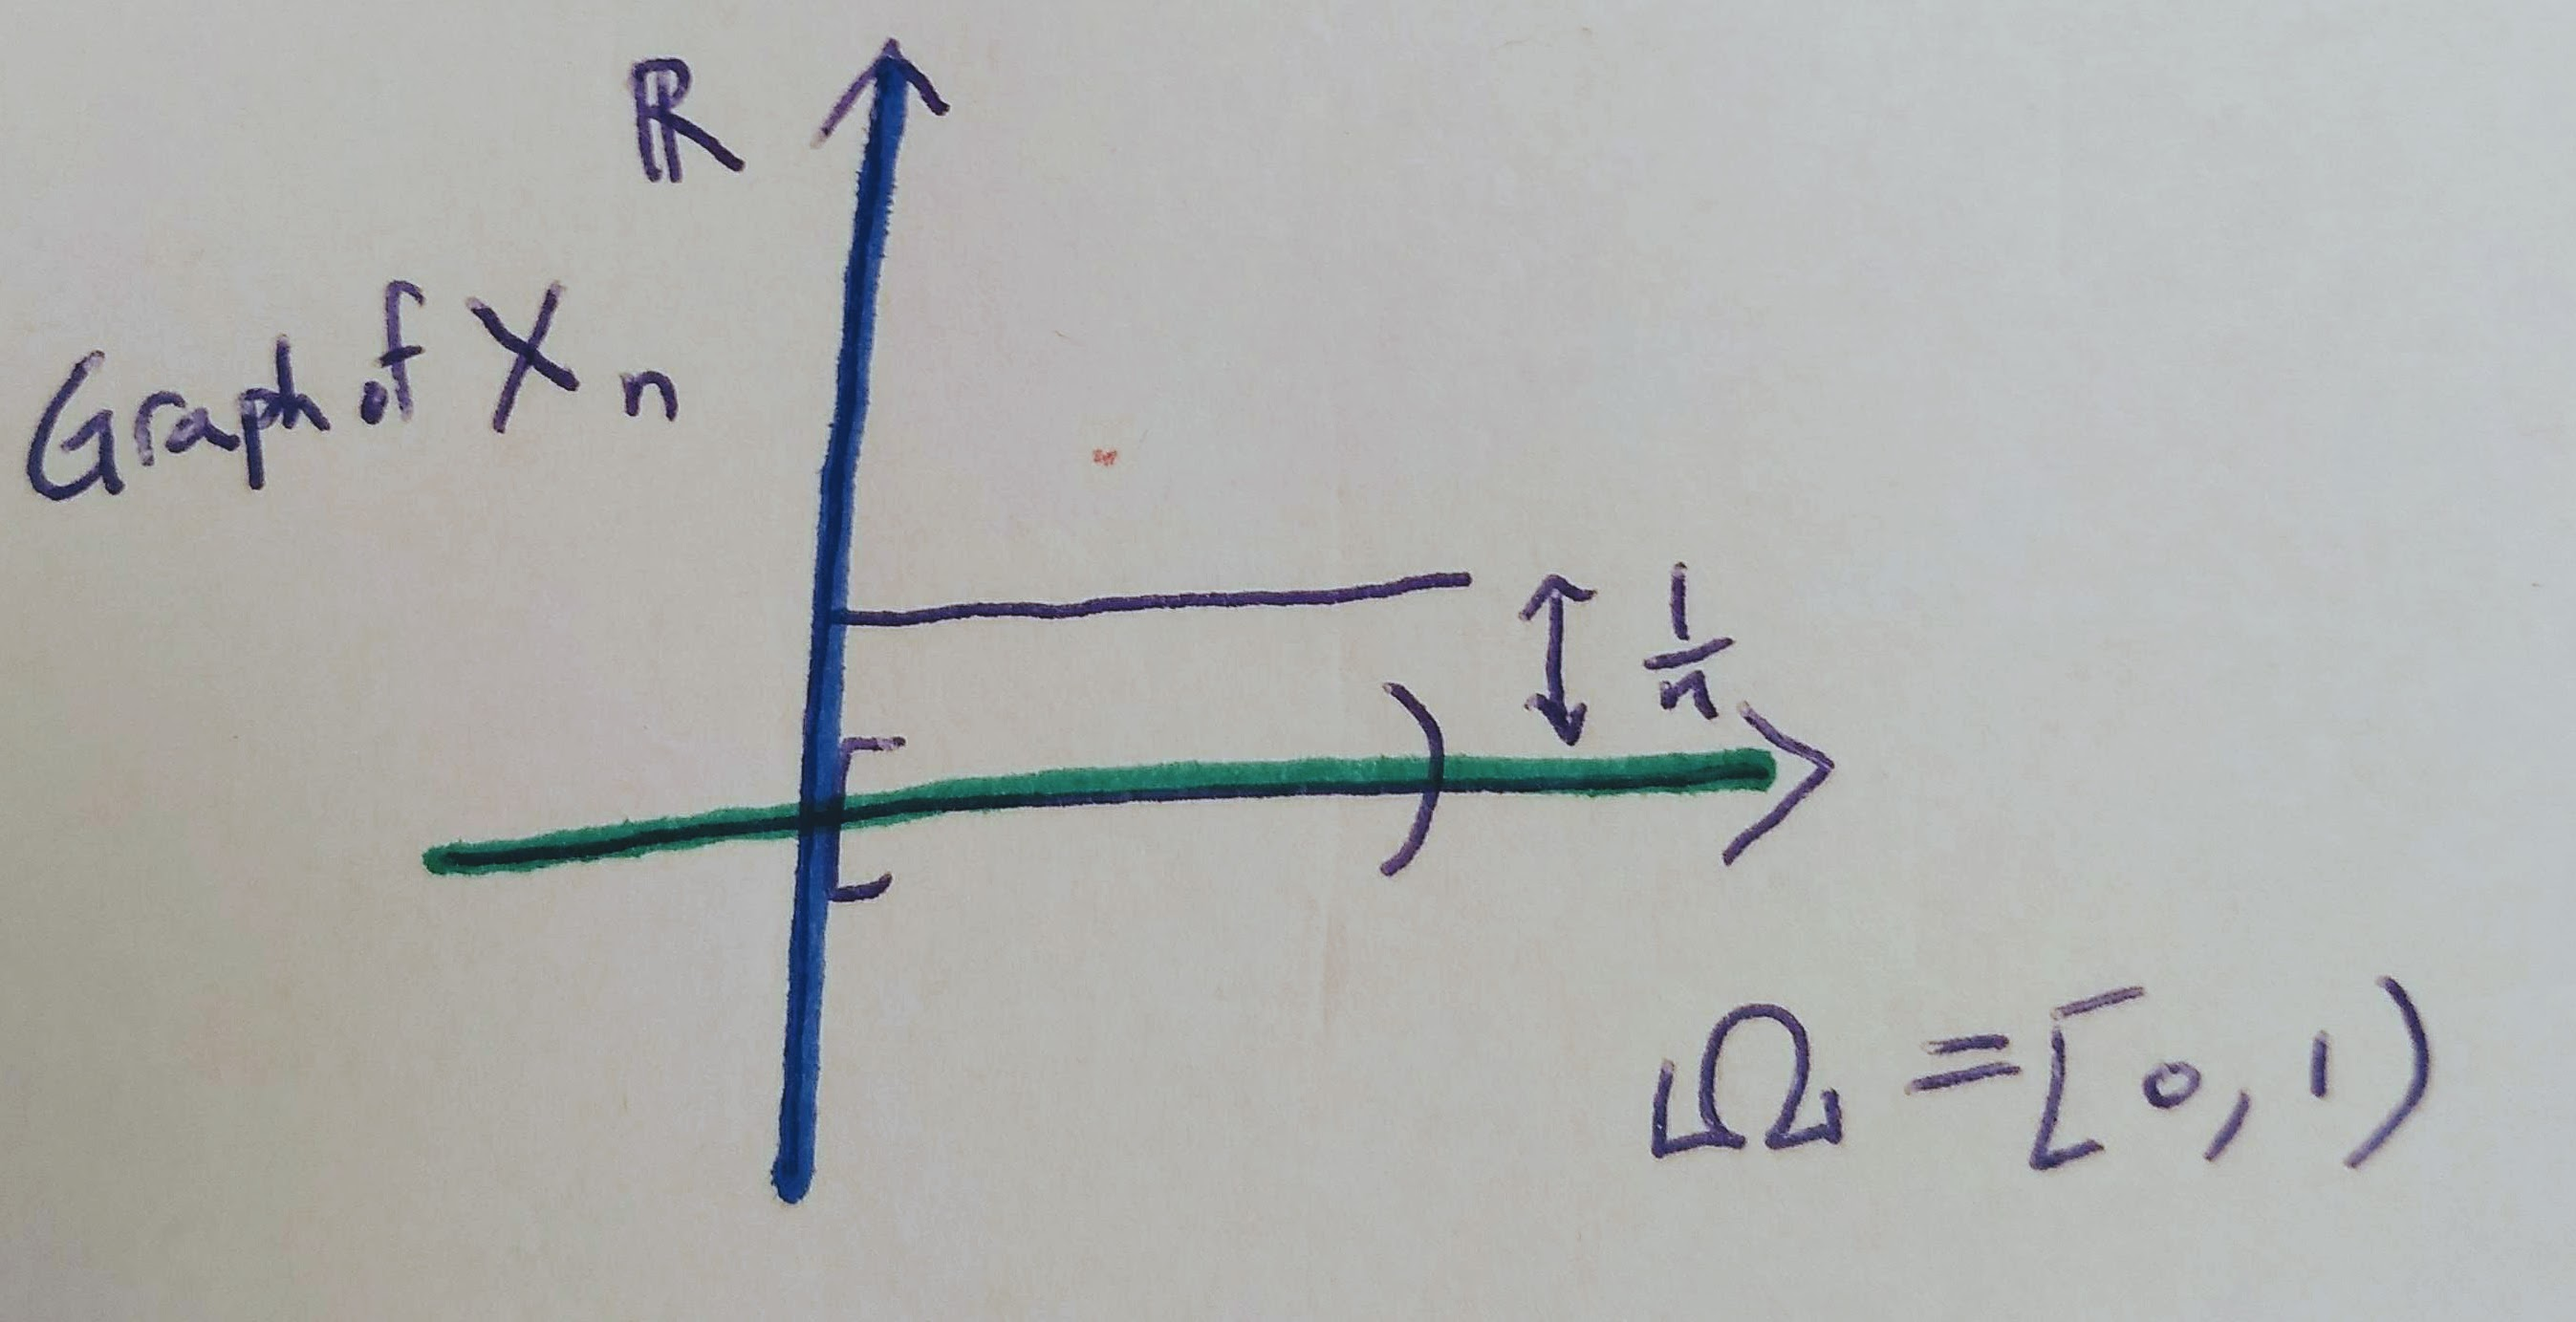
\includegraphics[width=0.5\linewidth]{figures/conv-dist-counter} 
\end{center}
however the limit of the cdfs at zero is equal to zero but the cdf of the limit at zero is one:
\begin{center}
	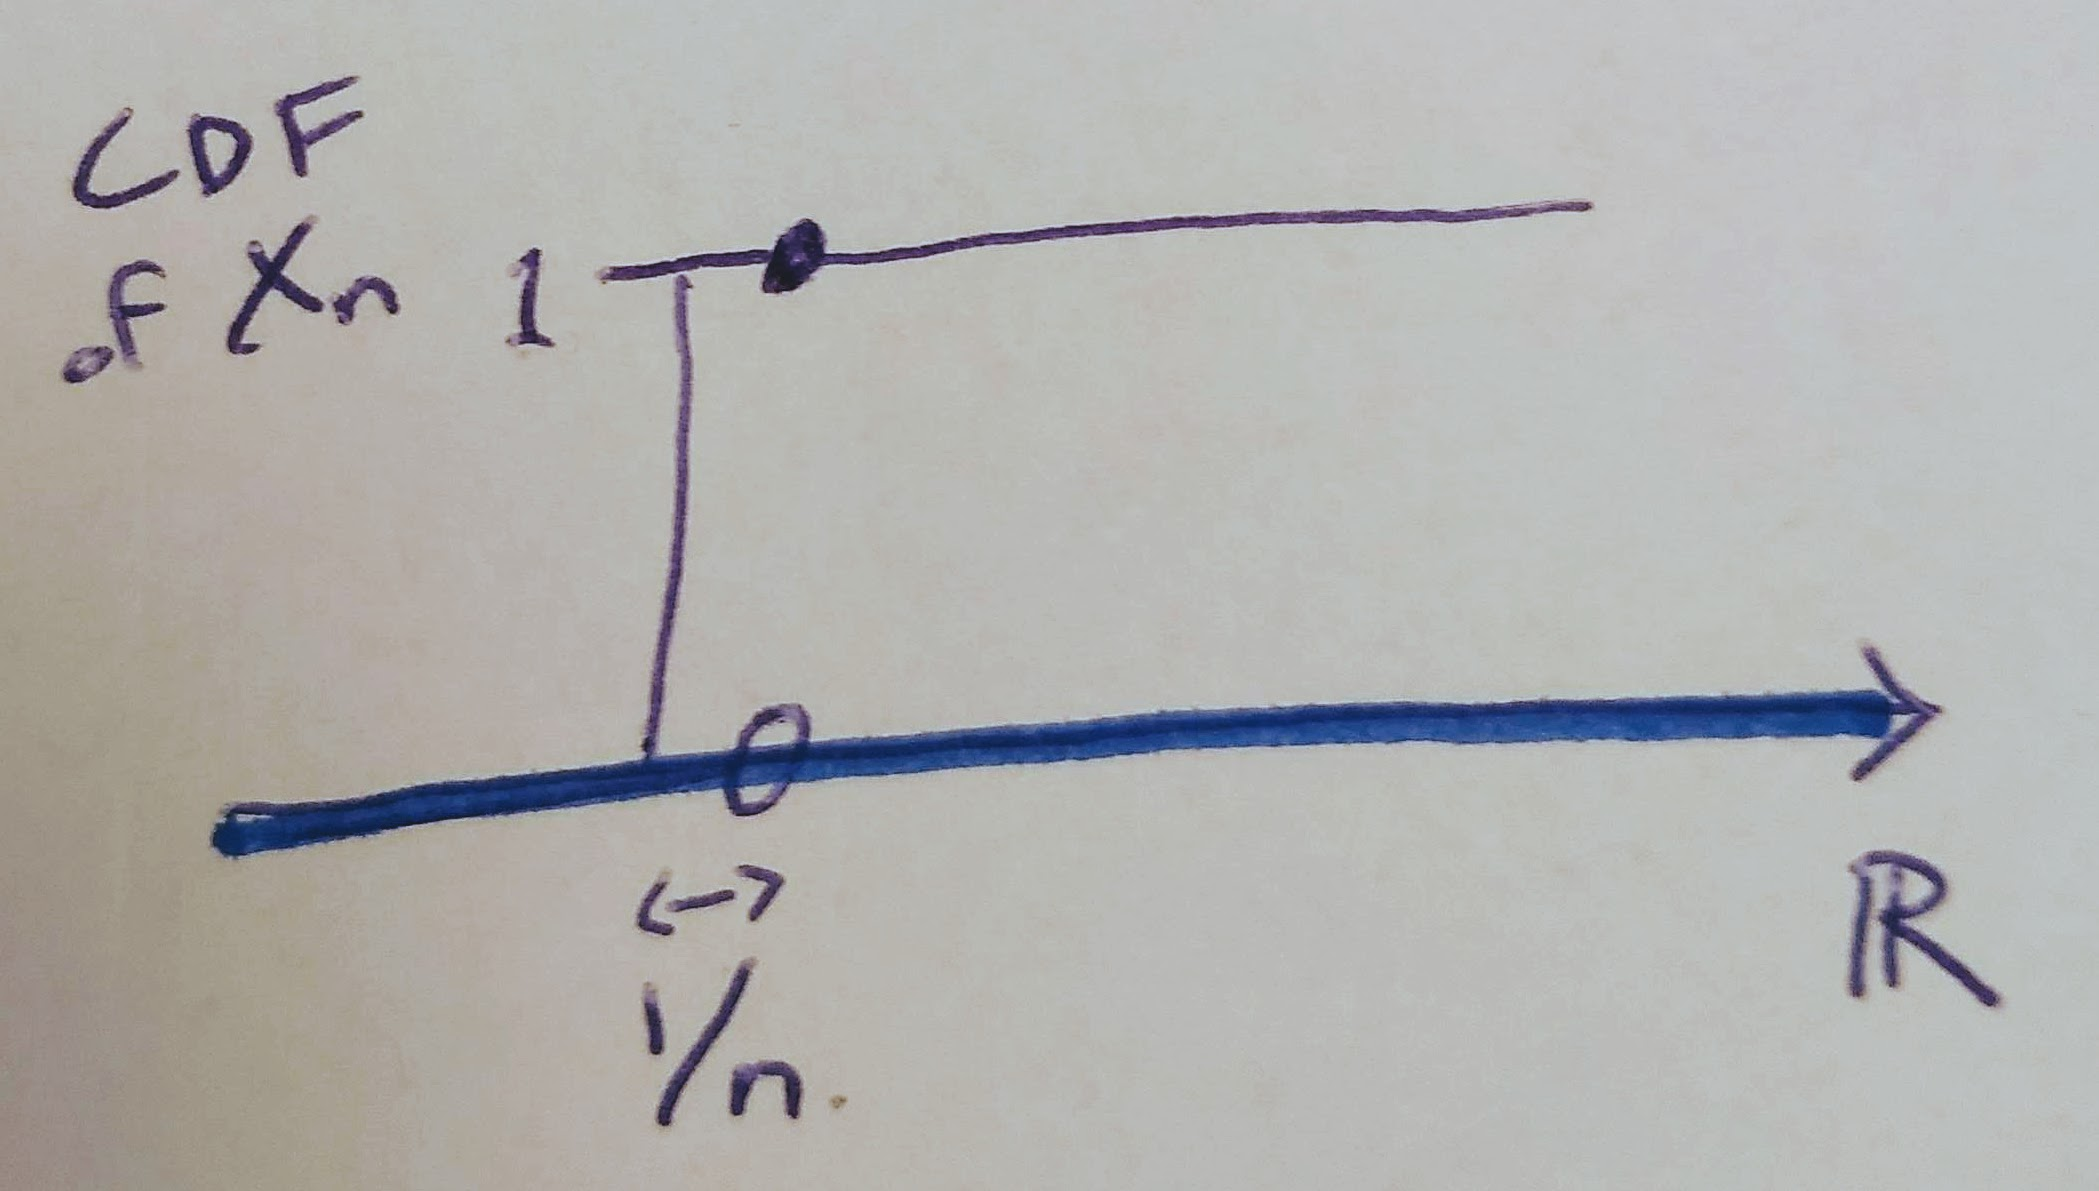
\includegraphics[width=0.5\linewidth]{figures/conv-dist-counter-2} 
\end{center}

\point{We can now write the CLT as follows:} if $X_1, X_2, \dots$ are idd with $E X_1^2 = 1$ and $\E X_1 = 0$, then:
\[ \frac{X_1 + \dots + X_n}{\sqrt{n}} \dcv Y, \]
where $Y$ is a standard normal. 

\point{Note:} this statement is not true in probability or a.s. (this can be proven using `Kolmogorov zero-one law').


\subsection{Overview of some properties of convergence of r.v.'s}

\point{Scheff\'e's theorem:} if $X_n$ have density $f_n$ such that $f_n \to f$ pointwise, where $f$ is the density of $X$, then $X_n \dcv X$.

\point{Proof:} dominated convergence.

\point{Continuous mapping I:}  if $g$ is continuous, $X_n \ascv X$, then $g(X_n) \ascv g(X)$. 

\point{Proof:} follows directly from definition of continuity.

\point{Continuous mapping II:} if $g$ is continuous, $X_n \dcv X$,  $g(X_n) \dcv g(X)$. 

\point{Proof:} trivial, provided you use the right equivalent definition provided by Portmanteau.

\point{Continuous mapping III:} if $g$ is continuous, $X_n \pcv X$, then $g(X_n) \pcv g(X)$. 

\point{Note:} this can be relaxed to accommodate a set of discontinuity $D$ as long as it has probability zero under the asymptotic distribution.

\point{Template for many results:} ``$X_n \stackrel{\square}{\longrightarrow} X$ and $Y_n \stackrel{\square}{\longrightarrow} Y$ implies $X_n \circ Y_n \stackrel{\square}{\longrightarrow} X \circ Y$'' where you should replace $\square$ and $\circ$ by any of these combinations (note that some combinations require extra assumptions):
\begin{enumerate}
  \item $\square = $a.s. and $\circ = +,$ or $-, *, /$.
  \item $\square = $p and $\circ = +,$ or $-, *, /$.
  \item $\square = $d and $\circ = +$, AND $X_n, Y_n, X, Y$ independent.
  \item $\square = $d and $\circ = +,$ or $-, *, /$, AND $Y = $ constant (``Slutsky's theorem'').
\end{enumerate}

\point{Example:} of why we have to be careful, especially with convergence in distribution. Let $Y, X, X_n$ all be iid N(0,1), and $Y_n = -X_n$. Then $X_n \dcv X$ and $Y_n \dcv Y$, but $X_n + Y_n \dcv 0 \stackrel{d}{\neq} X+Y$. Here we cannot use Slutsky's theorem because neither $X_n$ nor $Y_n$ converge to a constant.

\point{Main tools:} used to proved these results.
\begin{itemize}
  \item Subsequence characterization of convergence in probability: $X_n \pcv X$ if and only if for all subsequence $n_k$, there is a further subsequence $n_{k_i}$ such that $X_{n_{k_i}} \ascv X$.
  \item Skorokhod representation: suppose $X_n \dcv X$, then there exists $Y_n$ and $Y$ such that $Y_n, Y: \Omega \to \R$, $Y_n \deq X_n$, $Y \deq X$, and $Y_n \ascv Y$.
\end{itemize}


\subsection{Towards a proof of the CLT: generating functions}

To prove the CLT, we first need to look at tools that will help us study sums of random variable. These tools are called generating functions.  We go over generating functions because they are useful in many contexts, from theory to computation. 

\point{Why generating functions?} A generating function associates a function $G_X(s)$ to a random variable $X$. They are designed with two goals in mind:
\begin{enumerate}
	\item They \emph{characterize} certain classes of distributions. I.e. just as CDFs, if generating functions are equal (as functions), $G_X = G_Y$, then the corresponding random variables are equal in distribution, $X \deq Y$.
	\item The generating function of sums of independent random variables is the product of the individual generating functions: $G_{X+Y}(s) = G_X(s) G_Y(s)$. 
\end{enumerate}

\point{Specific applications} of generating functions:
\begin{enumerate}
	\item Most CLT proofs.
	\item The Fast Fourier Transform, one of the most important algorithms out there, is heavily based on generating functions. As an example of application of the Fast Fourier Transform, say you want to get the coefficient of the polynomial product $(a_n x^n + a_{n-1} x^{n-1} + \dots + a_0) \times (b_n x^n + b_{n-1} x^{n-1} + \dots + b_0)$. How long does it take to compute the coefficients of the product, $c_{2n} x^{2n} + c_{2n-1} x^{2n-1} + \dots +s c_0$? Naively, $O(n^2)$. Surprisingly, there exists a $O(n \log n)$ algorithm based on the Fast Fourier Transform.\footnote{Many references available online, e.g. \url{http://www.cs.uleth.ca/~benkoczi/files/fourier-excerpt.pdf}}
\end{enumerate}

\point{Types of generating function} that we will survey:
\begin{description}
	\item[Probability generating functions:] simplest to understand but only characterizes natural number valued random variables. We will start there for pedagogical reasons.
	\item[Moment generating functions:] which we already encountered when we talked about Chernoff bound in Section~\ref{sec:chernoff-revisited}. They are defined for some random variables beyond natural number valued ones, but not all.
	\item[Characteristic function:] which are always defined but will require a quick review on complex numbers. After covering those we will be ready for the proof of CLT.
\end{description}


\subsection{Probability generating functions}

\point{Restriction:} we only consider natural number valued random variables, i.e. $X : \Omega \to \{0, 1, 2, \dots \}$.

\point{Definition} of a probability generating function (PGF):
\[ G_X(s) = \E[s^X], \]
which in the context of a natural number valued random variables,
\[ G_X(s) = \sum_{i=0}^\infty \P(X = i) s^i. \]
Note that this sum might diverge for some values of $s$. For reason that will become clear soon, we elect to only define it when $\E|s^X| < \infty$ (the terminology is ``define $G$ for $s$ where the series is absolutely convergent'').\footnote{From real analysis, this is is true in a radius of at least one around the origin.}

\point{Exercise:} compute it for a Bernoulli. Then for a Poisson, with pmf for parameter $\lambda > 0$ given by \[p(n) = e^{-\lambda} \frac{\lambda^n}{n!} \1[n\in \N]. \]

\point{Solution for Bernoulli:} if $X \sim \Bern(\theta)$, then $G_X(s) = (1-\theta) + \theta s$.

\point{Solution for Poisson:} if $Y \sim \Poi(\lambda)$, the $G_Y(s) = e^{\lambda(s-1)}$. 

\point{Next:} do  probability generating functions indeed satisfy the two desiderata described in the last section (characterization and nice behaviour for sums)?

\point{First desiderata: nice behaviour with sums.} If $X$ and $Y$ are independent, the PGF of their sum is the product of the PGFs, $G_{X+Y} = G_X G_Y$.

\point{Proof:} by Tonelli:
\[ \E |s^{X+Y}| = \E | s^X s^Y | = \E | s^X | \E |s^Y|, \]
and the right hand side is finite by the absolute convergence assumption introduced in the definition. Then this mean we can apply Fubini and obtain:
\[ G_{X+Y}(s) = \E [s^{X+Y}] = \E [s^X] \E [s^Y] = G_X(s) G_Y(s). \]

\point{Exercise:} find the PMF of a sum of two independent (1) Bernoullis, (2) Poisson random variables with rates $\lambda_1$ and $\lambda_2$.

\point{Solution for Bernoulli:} $G_{X_1 + X_2}(s) = ((1-\theta) + \theta s)^2$.

\point{Solution for Poisson:} $G_{Y_1+Y_2}(s) = e^{(\lambda_1+\lambda_2)(s-1)}$.

\point{Observation: closure under sums.} Notice that for the Poisson example above, the PGF of $Y_1 + Y_2$ coincides with the PGF of a Poisson with mean parameter $\lambda = \lambda_1+\lambda_2$. This is not always the case: for example, for the Bernoulli example, we do not have this property. In the Poisson case, can we conclude right away that $Y_1 + Y_2$ is Poisson distributed? 

\point{Answer:} not yet! A priori, we do not know that some other distribution could yield the same PGF! But we will next argue that in fact this cannot happen!

\point{Second desiderata: characterization.} How to show that some other distribution cannot in fact yield the same PGF? By solving the following problem: give me a PGF $G$, and reconstruct the PMF, $p_k = \P(X = k)$. How to do this? Hint: view $G(s)$ as a polynomial. Start with reconstructing $p_0 = p(0)$.

\point{Solution:} \[ G(s) = p_0 + p_1 s + p_2 s^2 + p_3 s^3 + \dots. \]
Hence: $G(0) = p_0$. Next, how to get $p_1$?

\point{Trick:} If you know $G$ you can differentiate it! Get:
\[ G'(s) = p_1 + 2 p_2 s + 3 p_3 s^2 + \dots. \]
Hence: $G'(0) = p_1$.

\point{More generally:} \[ p_n = \frac{G^{(n)(0)}}{n!}. \]

\point{Application (reading):} branching processes. If a cell has a number of offspring that is Poisson-distributed with rate $\lambda$, and all its descendants recursively also have each iid Poisson-distributed descendants, what is the probability $p$ that the population eventually dies off? If $\lambda < 1$, $p=1$! For $\lambda \ge 0$, we can have $p < 1$, and even compute it from the PGF! Please read Section 5.4 in Grimmett and Stirzaker. 

\point{Application (optional):}  probability generating functions are important for the analysis of time series for count data, see for example \cite{zhu_negative_2010}.


\subsection{Moment generating function}

How to extend the ideas of last section to more general random variables? First try: moment generating functions (MGF).\footnote{Also known as the \emph{Laplace transform}, up to reparameterization.}

\point{Idea:} in the previous section, we looked at the expectation of $s^X$. If $X$ is non integer-valued, and we plug in a negative $s$, we get $\sqrt{-1}$. In an attempt to avoid complex numbers, the MFG $M(t)$ use the reparameterization $s = e^t > 0$ to avoid complex numbers, yielding:\footnote{However, as we will see soon, complex numbers are in some sense inevitable to do this in full generality.}
\[ M(t) = \E[e^{tX}]. \]
As with the PGF, this expectation may diverge for some values of $t$. As we shall see this is more problematic here since we get into situations where this is defined only at $t=0$, in which case the MGF clearly does not characterizes the distribution.

\point{Exercise:} compute the MGF of a standard normal distribution. Hint: complete the square to use known normalization of the normal density.

\point{Answer:} $\varphi(t) = \exp(t^2 / 2)$. 


\subsection{Characteristic function}

We would like to have a construction that is defined for all real random variables, and that has our two desiderata. 

\point{Idea:} in the last section we use the function $f(t) = e^t$, which is a function into an unbounded space, $f : \R \to [0, \infty)$. Let us try to map into a bounded space. To do this, let us wrap around the line into a circle as follows:
\begin{center}
	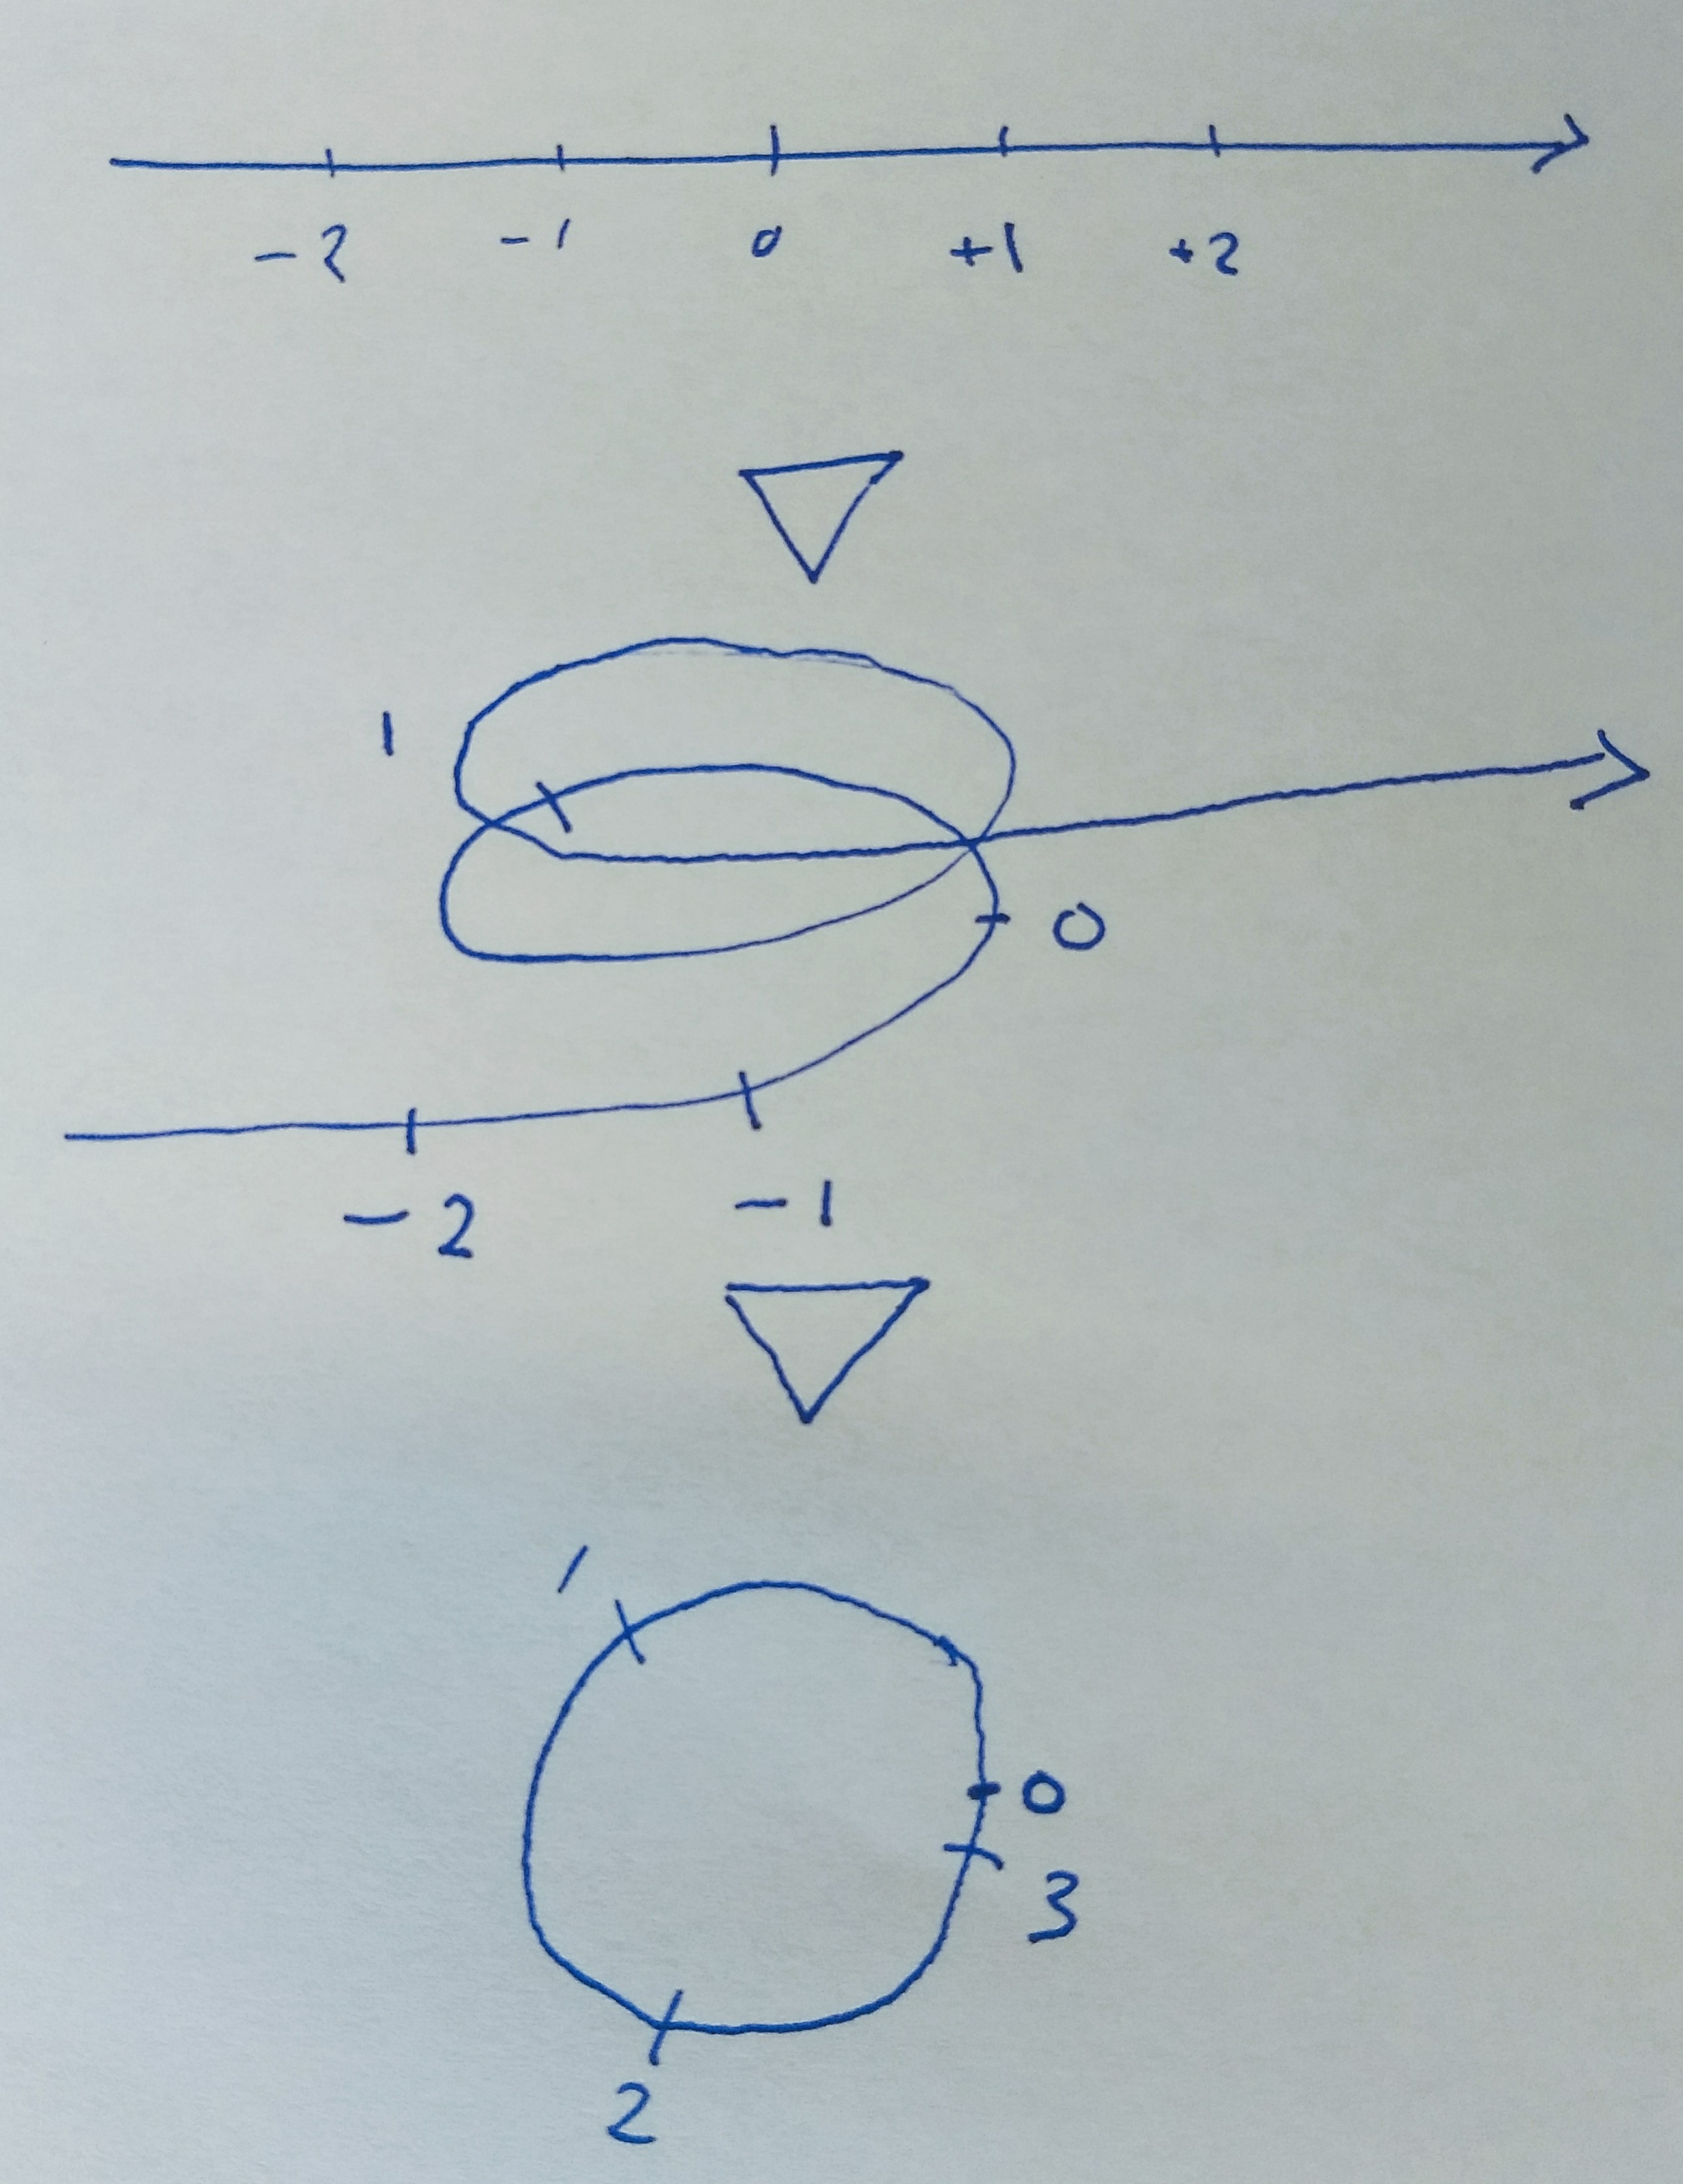
\includegraphics[width=0.3\linewidth]{figures/ch-fct} 
\end{center}
Let us formalize this construction using some light complex analysis.

\point{Recall:} a complex number $c \in \C$ can be written as: $c = a + b i$ where $i = \sqrt{-1}$, i.e. such that $i^2 = -1$.

\point{Definition:} a complex random variable is defined as $Z = X + iY$, and we define its expectation as $\E Z = \E X + i\E Y$.

\point{Some nice tricks with Taylor series:} let us say $x$ is real.  
\begin{align*}
	e^{ix} &= 1 + (ix) + \frac{(ix)^2}{2!} + \frac{(ix)^3}{3!} + \dots \\
	&= 1 + (ix) - \frac{x^2}{2!} - \frac{i(x)^3}{3!} + \dots \\
	&= (1 - \frac{x^2}{2!} + \dots) + i(x - \frac{x^3}{3!} + \dots) \\
	&= \cos x + i \sin x.
\end{align*}
So, $|e^{ix}| = 1$ and we have something like we wanted in our picture above! Now clearly, if I give you some real value random variable $Y$,
\[ \E[e^{itY}] = \E[\cos(tY)] + i \E[\sin(tY)], \]
is always well defined and finite since $\sin$ and $\cos$ are bounded!

\point{Success!} Define the characteristic function as $\varphi_Y(t) = \E[e^{itY}]$. It satisfies both our desiderata!

\point{Proof:} See Durrett. Based on the following idea: if I give you $\varphi$, you can reconstruct $Y$ via the formula
\[ \P(Y \in (a, b]) = \lim_{T\to\infty} \int_{-T}^T \frac{e^{-ita} - e^{itb}}{it} \varphi(t) \ud t. \]


\subsection{Further properties of characteristic functions}

\point{Property P0:} $X_n \dcv X \Longleftrightarrow \varphi_{X_n}(t) \to \varphi_{X}(t)$.

\point{Property P1:} $\varphi_X(0) = 1$

\point{Property P2:} $|\varphi_X(t)| \le 1$

\point{Proof:} complex version of Jensen. If $g$ is convex, then $g(\E X) \le \E[g(X)]$. Take $g(x) = |x|$.

\point{Property P3:} $\varphi_X(t)$ is always continuous (viewed as a function of $t$). 

\point{Proof:} take $t_n \to t$.
\begin{align*}
&\Longrightarrow i t_n X \to i t X \text{ a.s.}, \\
&\Longrightarrow \exp(i t_n X) \to \exp(i t X) \text{ a.s.}, 
\end{align*}
Where the last implication follows by continuity of $\exp$. Finally,
\[ \varphi_X(t_n) = \E[e^{it_n X}] \ascv \E[e^{itX}] = \varphi_X(t), \]
by using DCT with $|e^{it_n X}| = 1$.

\point{Property P4:} If $\E|X| < \infty$, then $\varphi_X(t)$ has a derivative and 
\begin{align*} 
\frac{\ud}{\ud t} \varphi_X(t) &= \frac{\ud}{\ud t} \E[ e^{itX} ] \\
&= \E[\frac{\ud}{\ud t} e^{itX}] \text{ (will use our earlier swap result)} \\
&= \E[iX e^{itX}], 
\end{align*}
and in particular,
\[ \E X = \frac{\varphi_X(0)}{i}. \]

\point{Proof:} we use the result in Section~\ref{sec:exchange}, which we copy here for convenience.

\point{Theorem for swaps:} suppose 
\begin{enumerate}
	\item $g(\cdot, \theta)$ is integrable for all $\theta \in [a, b]$, 
	\item $g(x, \theta)$ is differentiable for all $x$ and $\theta$, 
	\item there is an integrable envelope $h(x)$ such that $|\ud g(x, \theta) / \ud \theta| \le h(x)$ for all $x$ and $\theta$,
\end{enumerate}
then both sides of the equation below are well defined and equal:
\[ \frac{\ud}{\ud \theta} \int g(x, \theta) \mu(\ud x) = \int \frac{\ud}{\ud \theta} g(x, \theta)   \mu(\ud x). \]

\point{Back to proof:} we use our earlier result with $x = \omega$,  $\theta = t$, 
\[ g(\omega, t) = e^{itX(\omega)}, \]
and envelope
\[ h(\omega) = |X(\omega)|. \]
For condition 1, we have
\[ \int | g(\omega, t) | \P(\ud \omega) = \int 1 \P(\ud \omega) = 1. \]
For condition 2, we have indeed that $e^{itx} = \cos(tx) + i \sin(tx)$ is continuous for all $x$ and $t$. 
For condition 3, we have $\E|X| < \infty$ by assumption.

\point{Property P5:} more generally, if $\E[|X^k|] < \infty$, 
\[ \varphi^{(k)}(t) = \E[(iX)^k e^{itX}]. \]
As a consequence, we get the following important special case: if $\E X^2 < \infty$, then by Taylor's Theorem (Peano form) applied around zero, there exists a function $h$ such that $h(t) \to 0$ as $t\to 0$ with:
\[ \varphi(t) = 1 + it\E X - \frac{1}{2} t^2 \E[X^2] + h(t) t^2. \]

\point{Factoid:} the characteristic function of a standard normal distribution is 
\[ \varphi(t) = e^{-\frac{1}{2} t^2}. \]
This will be the last ingredient needed for proving the CLT. This from should not be a surprise given the closely related form for the MGF. However proving this is surprisingly tricky (requires contour integration methods from complex analysis). 


\subsection{Proof of basic CLT}

\point{Theorem:} if $X_1, X_2, \dots$ are idd with $E X_1^2 = 1$ and $\E X_1 = 0$, then:
\[ \frac{X_1 + \dots + X_n}{\sqrt{n}} \dcv Y, \]
where $Y$ is a standard normal. 

\point{Proof:} let us fix an arbitrary $t$, and start by looking at only one variable $X_1$. We have, by P5, that 
\[ \varphi_{X_1}(t) = 1 - \frac{1}{2} t^2 + h(t) t^2, \]
where all we know about $h$ is that $h(t) \to 0$ when $t \to 0$.

\point{Trick:} to look at a normalized sum, note
\begin{align*}
\varphi_{aX}(t) &= \E[ e^{it(aX)}] \\
&= \E[ e^{i (at) X} ] \\
&= \varphi_{X}(at).
\end{align*}

\point{Apply trick to proof:} to get the characteristic function of $\frac{S_n}{\sqrt{n}} = \frac{X_1 + \dots + X_n}{\sqrt{n}}$,
\begin{align*}
\varphi_{S_n/\sqrt{n}}(t) &= ( \varphi_{X_1}(t/\sqrt{n}))^n \\
&= \left(1 - \frac{1}{2} (t/\sqrt{n})^2 + h(t/\sqrt{n}) (t/\sqrt{n})^2\right)^n \\
&= \left(1 - \frac{(-t^2/2) + h(t/\sqrt{n}) t^2}{n} \right)^n
\end{align*}

\point{From real analysis:} $e^x = \lim_{n\to\infty} (1 + x/n)^n$.

\point{Extension:} if $x_n \to x$, then $e^x = \lim_{n\to\infty} (1 + x_n/n)^n$.

\point{Applying this to our setup:} 
\begin{align*}
x &= -t^2/2 \\
x_n &= -t^2/2 + h(t/\sqrt{n}) t^2.
\end{align*}
we get $\lim_{n\to\infty} \varphi_{S_n/\sqrt{n}}(t) = e^{-t^2/2}$.

\point{Conclusion:} by P0, it follows that 
\[ S_n / \sqrt{n} \dcv Z, \]
where $\varphi_Z(t) = e^{-t^2/2}$. By our characterization result and the factoid from last section, it follows that $Z$ is a standard normal random variable.


\subsection{CLT: multivariate version}

\point{Setup:} suppose now we have a sum of iid copies of a $d$-dimensional mean zero random \emph{vector}, $X_1 = (X_{1,1}, X_{1,2}, \dots, X_{1,d})$. The interesting bit is that we do \emph{not} assume independence across the $d$ dimensions. 

\point{Goal:} We are interested in approximating the distribution of the sum of vectors $\sum_{i=1}^n X_i$, where $X_i = (X_{1,i}, X_{i,2}, \dots, X_{i,d})$. We assume $X_i \deq X_j$ for all $i,j$ and that the $X_i$ are independent (across $i \in \{1, \dots, n\}$, but still allowing for dependence within one vector across dimensions $k \in \{1, \dots, d\}$).

\point{Assumption:} we do need to assume some kind of second moment assumption. In the vector context, this becomes $\E|X_{1,k} X_{1,k'}| < \infty$. This reduces to our usual condition if $d=1$, so no surprise here.

\point{Theorem:} under the above assumptions,
\[ \frac{X_1 + X_2 + \dots + X_n}{\sqrt{n}} \dcv Z, \]
but this raises a few questions: (1) what does convergence in distribution mean for random vectors? (2) what is the limiting random vector $Z = (Z_1, Z_2, \dots, Z_d)$, and (3) how does this limiting object takes into account the dependence structure within each $X_i$?

\point{Convergence in distribution of random vectors:} here the trick is to recall that we have the following definition of univariate convergence in probability (by Portmanteau): $Y_n \dcv Y$ if
\[ \E[g(Y_n)] \to \E[g(Y)], \]
for all bounded continuous $g$. Note that this ``univariate'' definition actually immediately generalizes verbatim to random vectors!

\point{Limiting object:} recall that a mean-zero normal can be thought of as a density proportional to exponentiating a polynomial of degree two (with leading coefficient negative to ensure integrability):
\[ f(x) \propto \exp(-a x^2) = \exp(- x a x), \]
for $a > 0$. The density of the limiting object is a generalization of the above given by
\[ f(x) \propto \exp(- x' A x), \]
where $x'$ is a transpose of dimension $1$ by $d$, $A$ is $d$ by $d$, and $x$ is $d$ by $1$, therefore the product is a scalar. Here is what the density looks like:
\begin{center}
	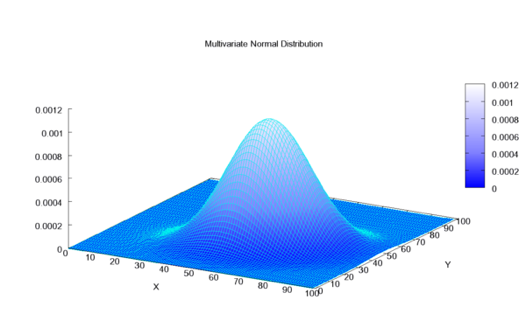
\includegraphics[width=0.5\linewidth]{figures/mvn} 
\end{center}
To ensure integrability, we ask that the matrix $A$ be such that $x' A x$ be positive  for all $x \in \R^d$, a condition called \emph{positive definiteness}. One fact we will assume from linear algebra is that $A$ being positive definite implies it is invertible. 

\point{Multivariate normal:} it turns out the reparameterization $\Sigma = 2A^{-1}$, called the covariance matrix, is more interpretable, because then $\E[Z_{d} Z_{d'}] = \Sigma_{d,d'}$. Moreover, the normalization constant has a closed form, which yields the standard expression for the \emph{multivariate normal distribution}:
\[ f(x) = \frac{1}{\sqrt{(2\pi)^d |\Sigma|}} \exp\left(-\frac{1}{2} x' \Sigma^{-1} x\right). \]

\point{How to compute $\Sigma$ in the multivariate CLT:} $\E[Z_{d} Z_{d'}] = \E[X_{1,d} X_{1,d'}]$, i.e. again we can just look at matching the first two moments of one random vector.  

\point{Proving tool: Cram\'er-Wold device.} Let $Y$ and $Y_n$ be any random vectors. Then $Y_n \dcv Y$ if and only if for all scalar $v \in \R^d$, $Y_n' v \dcv Y' v$.


\subsection{CLT: self-centered version}\label{sec:clt-non-centered}

So far we have assumed the $X_i$ have zero mean. This can always be done without loss of generality but it is often useful to memorize the formula that does that for you:
\[ \sqrt{n}(\bar X_n - \mu) \to N(0, \Sigma), \]
where the $d$ dimensional random vector $\bar X_n$ is the \emph{empirical average}, $\bar X_n = (X_1 + X_2 + \dots + X_n) /n$, the $d$-dimensional vector $\mu$ is the mean, $\mu = \E[X_1]$, and the matrix $\Sigma$ is the covariance matrix, which in the non-centered case is $\Sigma_{d,d'} = \E[ (X_{1,d} - \mu_d) (X_{1,d'} - \mu_{d'}) ]$.


\subsection{Delta method}

\point{Motivation.} Recall that the sample variance is given by
\[ S_n^2 = \frac{1}{n} \sum_{i=1}^n (X_i - \bar X_n)^2 \]
and has the property that $S_n^2 \ascv \var X_1$. Can we use the CLT to justify a normal approximation of the distribution of $S_n^2$ for $n$ large? Convince yourself that it does not ``quite'' fit the statement of the CLT.

\point{Idea:} start with a CLT on the 2-d vectors $Y_i = (X_i, X_i^2)$:
\[ \sqrt{n}(\bar Y_n - \mu) \to N(0, \Sigma), \]
where, using the shorthand $\alpha_j = \E X_1^j$, $\mu = (\alpha_1, \alpha_2)$, $\Sigma_{1,1} = \alpha_2 - \alpha_1^2$, $\Sigma_{1,2} = \Sigma_{2,1} = \alpha_3 - \alpha_1 \alpha_2$, and  $\Sigma_{2,2} = \alpha_4 - \alpha_2^2$. Then we will transform this CLT into the convergence statement we want, using a differentiable function $\phi$. 

\point{Example:} $S_n^2 = \phi(\bar Y_n)$, where $\phi(x, y) = y - x^2$. 

\point{Goal:} get a new asymptotic approximation on $\phi(\bar Y_n)$ given a known asymptotic approximation on $\bar Y_n$. We already know from the continuous mapping theorem that $\phi(\bar Y_n) \ascv \phi(\mu)$. This suggests looking at convergence in distribution of 
\begin{align}\label{eq:clt-for-delta}
\sqrt{n}(\phi(\bar Y_n) - \phi(\mu)).
\end{align}
How to tackle the weak limit of this sequence of random variables?

\point{Technique:} Taylor expansion of $\phi$ around the mean $\mu$, 
\[\phi(\bar Y_n) = \phi(\mu) + \phi'(\mu)(\bar Y_n - \mu) + \dots.\]
Informally plugging the above into Equation~(\ref{eq:clt-for-delta}), we get
\[ \sqrt{n}(\phi(\bar Y_n) - \phi(\mu)) \approx \phi'(\mu) (\bar Y_n - \mu). \]

\point{Theorem (delta method):} if $\phi : \R^k \to \R^m$ is differentiable at $\mu$, and 
\[ \sqrt{n}(T_n - \mu) \dcv T \] 
then
\[ \sqrt{n}(\phi(T_n) - \phi(\mu)) \dcv \phi'(\mu) T, \] 
where $\phi'$ is the $m$ by $k$ matrix of partial derivatives, $\phi'_{i,j}=\partial_i \phi_j$.

\point{Proof:} if assuming continuous differentiation, a simple application of the mean value theorem, continuous mapping and Slutsky. See e.g. van der Vaart for the full version.

\point{Exercise:} complete the motivation, showing that, \[ \sqrt{n}(S^2_n - \var X_1) \dcv Z, \]
where $Z$ is a normal with mean zero and variance $\alpha_4 - \alpha_2^2$.


\subsection{LLNs and CLTs under relaxed assumptions}

\point{Removing all independence assumptions:} so far we have allowed dependences between components of random vectors but not across separate random vectors. This can be considerably relaxed. One of the most useful relaxation is based on \emph{Markov chains}. We sketch here the results in their simplest possible form, and will talk in more depth later.

\point{Markov chains, discrete case:} consider a list of random variables $X_1, X_2, \dots$ with a distribution constructed as follows:
\[ \P(X_1 = x) = v_x, \]
where $v = (v_1, v_2, \dots, v_N)$ is a known vector called a initial distribution, $x \in \{1, 2, \dots, N\}$, and
\[ \P(X_i = x' | X_{i-1} = x) = M_{x,x'}, \]
where $M = (M_{x,x'})$ is a known $N$ by $N$ matrix called the transition matrix. 

\point{Theorem:} if $M^N$ has no zero entries,\footnote{There are far more general conditions, but they need more setup. We will get to the more general conditions later.} there exists a distribution $\pi$ such that we have the following LLN:
\[ \frac{1}{n} \sum_{i=1}^n f(X_i) \ascv \mu = \int f(x) \pi(\ud x). \]
and CLT:
\[ \sqrt{n}(\bar X_n - \mu) \dcv Z, \]
where $Z \sim N(0, \sigma^2)$.

\point{What is $\pi$?} This time it is more complicated than the distribution of one of the $X_i$'s, since the distributions are not identical! But it turns out we can still get a lot of knowledge about $\pi$, called the \emph{stationary distribution}. Similarly for $\sigma^2$, called the asymptotic variance. To be continued when we talk about Markov chains in more depth. 


\subsection{Convergence in $L^p$}

\point{Definition:} $\E |X_n - X|^p \to 0$, denoted $X_n \lpcv X$. Special cases are called ``convergence in mean'' (for $p=1$) or ``convergence in mean square'' (for $p=2$).

\point{Exercise:} show $X_n \lpcv X$ implies $X_n \pcv X$. Hint: use Markov's inequality.

\point{Exercise:} the converse is not true. Hint: use the example from Section~\ref{sec:exchange-lim}. 

\point{Hierarchy:} This extends Section~\ref{sec:conv-types-big-picture} into:
\begin{center}
	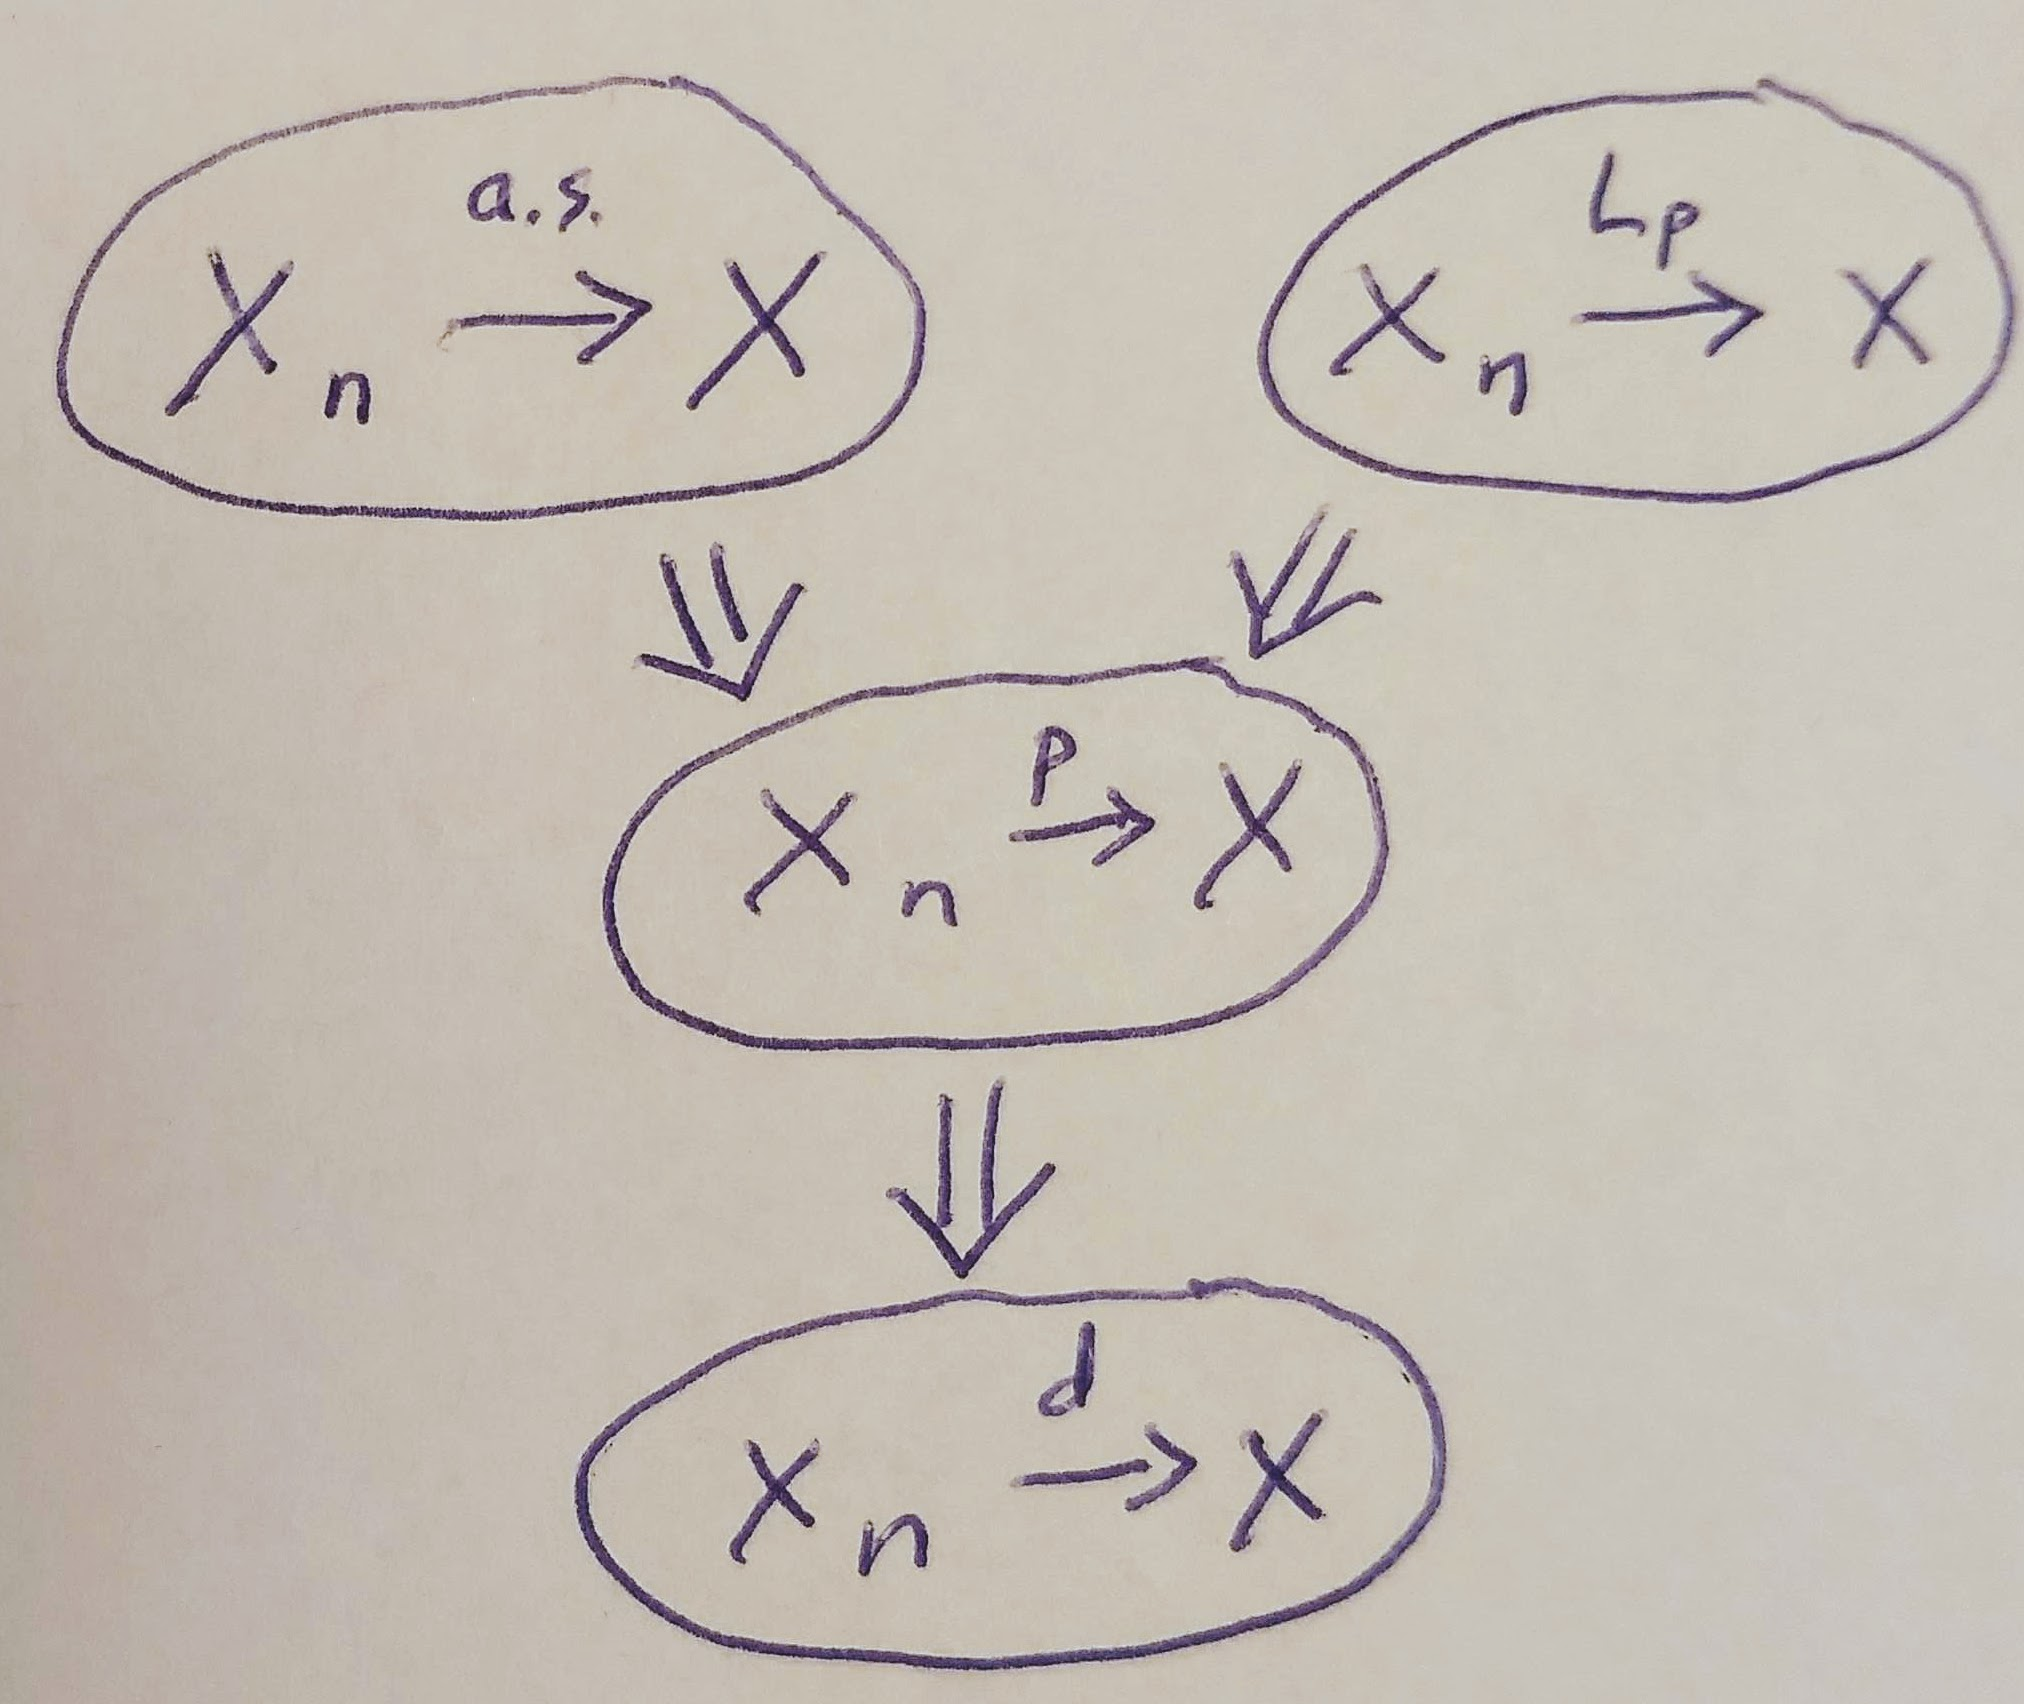
\includegraphics[width=0.5\linewidth]{figures/types-of-conv} 
\end{center}

\point{Partial converse:} back to the relation between convergence in probability and convergence in mean. For $p=1$, we have $X_n \pcv X$ implies $X_n \lpcv X$ if and only if they are \emph{uniformly integrable}, defined as: for all $\epsilon > 0$, there is $K > 0$ such that $\sup \E[|X_n| \1(|X_n| \ge K)] \le \epsilon$. 

\point{Exercise:} check that indeed the example from Section~\ref{sec:exchange-lim} is not uniformly integrable.


\section{Poisson theory}

\subsection{Poisson convergence}

\point{Motivation:} consider the following historical dataset, containing the number of accidental horse-kick deaths per year in the Prussian army in the 1881--1896 period: 7 deaths in 1881, 1 in 1882, 3, 2, 7, 6, 1, 3, 2, 2, 6, 4, 4, 1, 6, 2. Question: can we approximate the probability that there are no deaths in 1897?

\point{Proposition:} if for some constant $\lambda > 0$,  $X_n \sim \Bin(n, \lambda/n)$ and $X \sim \Poi(\lambda)$, then $X_n \dcv X$.

\point{Proof:} a short proof consists in using characteristic functions. As an exercise, show that the characteristic functions of the binomial random variables in the sequence are given by 
\[ \varphi_{X_n}(t) = \left( 1 - \frac{\lambda}{n} + \frac{\lambda}{n} e^{it} \right)^n, \]
and the characteristic function for the Poisson is given by:
\[ \varphi_{X}(t)  = \exp(\lambda(e^{it} - 1)). \]
It is easy to show that for all $t$, $\varphi_{X_n}(t) \to  \varphi_{X}(t)$. 

\point{Exercise:} show how to solve the motivation problem using this proposition.

\point{Solution:} for a Poisson distribution, the maximum likelihood and moment matching coincide, so we can fit the parameter as follows $\hat \lambda \approx \frac{1}{16} (7 + 1 + \dots + 2) = 3.5625$. This yields \[\P(X = 0) = e^{-\hat \lambda} \hat\lambda^0 / 0! \approx 2.8\%. \] 

\point{Generalization using ``triangular arrays:''} let $X_{n,m}$ denote an array with the variables in each row being independent:
\begin{itemize}
  \item $X_{2,1}, X_{2,2}$ are independent.
  \item $X_{3,1}, X_{3,2}, X_{3,3}$ are independent.
  \item etc.
\end{itemize}
Assume $X_{n,j} \sim \Bern(p_{n,j})$, where
\begin{enumerate}
  \item we have convergence of row sums to $\lambda$: $\lim_{n\to\infty} \sum_{j=1}^n p_{n,j} = \lambda$,
  \item and as we look at larger and larger row indices $n$ the Bernoulli probabilities become uniformly rare across the columns $j$: $\lim_{n\to\infty} \max_j p_{n,j} = 0$.
\end{enumerate}
Then: $S_n = X_{n,1} + X_{n,2} + \dots + X_{n,n}$ is such that $S_n \dcv X$, where $X \sim \Poi(\lambda)$.

\point{Exercise:} show that the earlier result is a special case of this one.

\point{Proof:} based on the Stein-Chen coupling method. See textbook p. 459. 


\subsection{Poisson processes: motivation, definition and construction}

\point{Prerequisite definition:} a \emph{Radon-Nikodym derivative} (RN) is like a density, but where we build a measure instead of a probability measure. Compare:
\begin{itemize} 
  \item The probability measure $\nu$ has density $f \ge 0$ with respect to a measure $\mu$ if \[ \nu(A) = \int_A f(x) \mu(\ud x). \]
  \item The measure $\nu$ has RN derivative $f \ge 0$ with respect to a measure $\mu$ if \[ \nu(A) = \int_A f(x) \mu(\ud x). \]
\end{itemize}

\point{Poisson process---motivation and connexion to Poisson convergence:}\footnote{Reference for the Poisson process: the best reference in my opinion for this part of the material is the beautiful short monograph by Kingman (1993), ``Poisson Processes.''}  
\begin{itemize}
  \item Let $n$ denote the number of nucleotides in your genome (about 3e9 base pairs). 
  \item Say you are exposed to a small dose of radiation. 
  \item Let $Y_i$ denote the indicator that nucleotide $i$ in a cell mutates. 
  \item Say $Y_i \iidsim \Bern(1e-9)$, and let $S_n = Y_1 + Y_2 + \dots + Y_n$.  
  \item By the Poisson convergence section, $S_n$ is approximately Poisson distributed, with rate parameter $\lambda$.
  \item Now let us view the genome as one line segment $[0, 3]$ (a continuous approximation of the discrete DNA strand). 
  \item What is the approximate probability of the number of mutation in the first half of the genome? Last quarter? Are those independent?
\end{itemize}
\begin{center}
	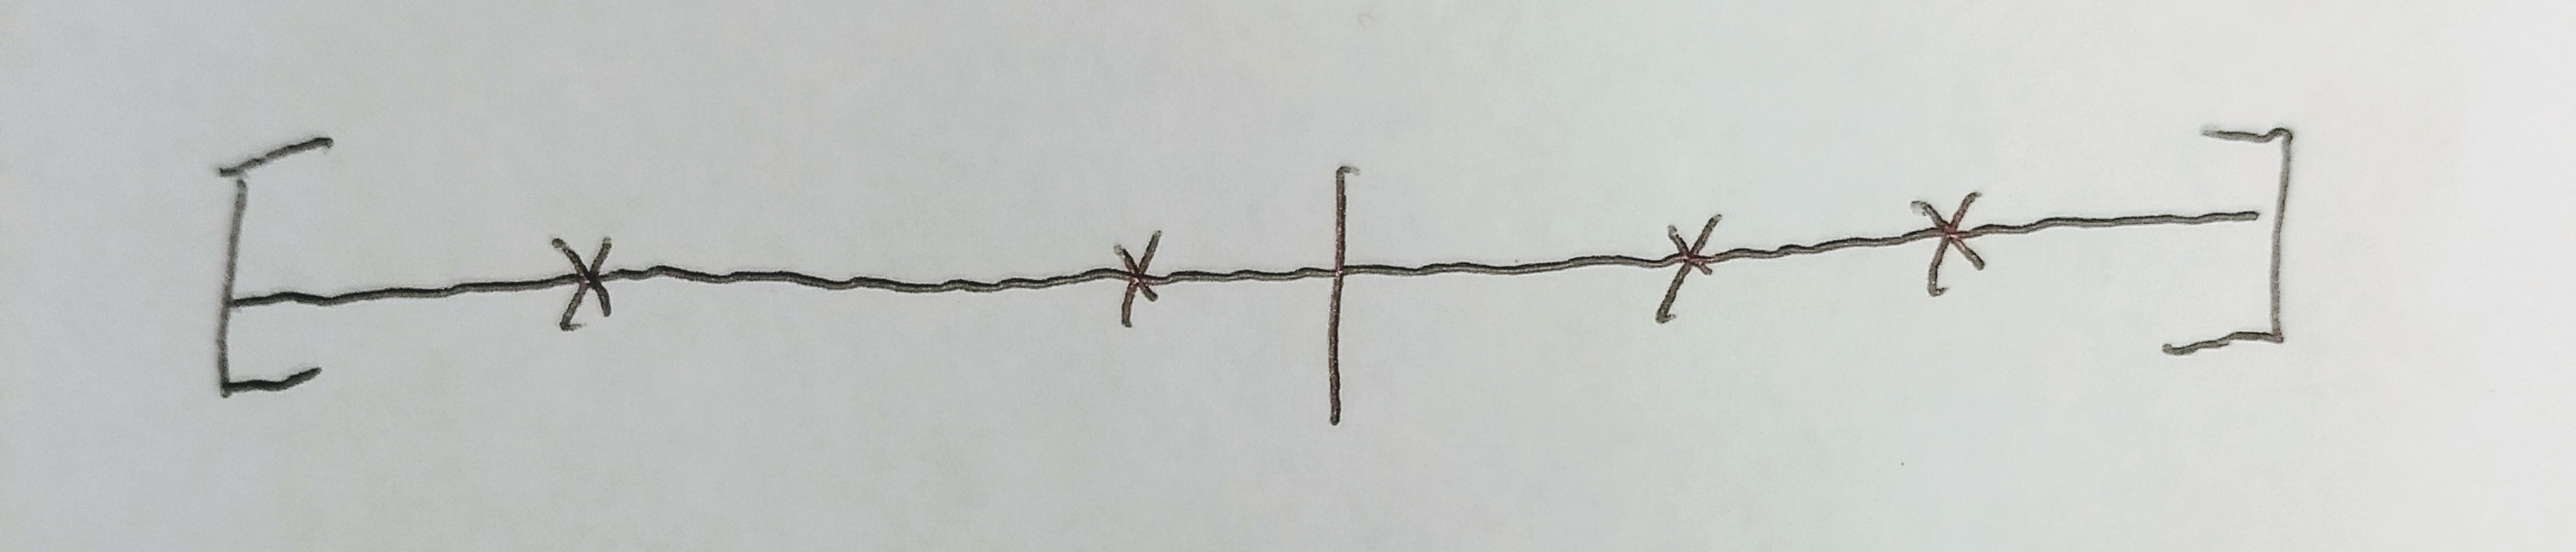
\includegraphics[width=0.5\linewidth]{figures/pp-genome} 
\end{center}

\point{Poisson distribution vs.\ process:} the distribution only keeps track of the total number of mutation, while the process keeps track of where they occur (equivalently, the number in \emph{any} subset of genome).

\point{Notation:} 
\begin{itemize}
  \item $\ppspace$: the space in which each point sits in (for example, the interval $[0, 3]$ approximating the genome).
  \item For $A \subset \ppspace$, let $N_A$ denote the random number of points that fall in $A$.
\end{itemize}
\begin{center}
	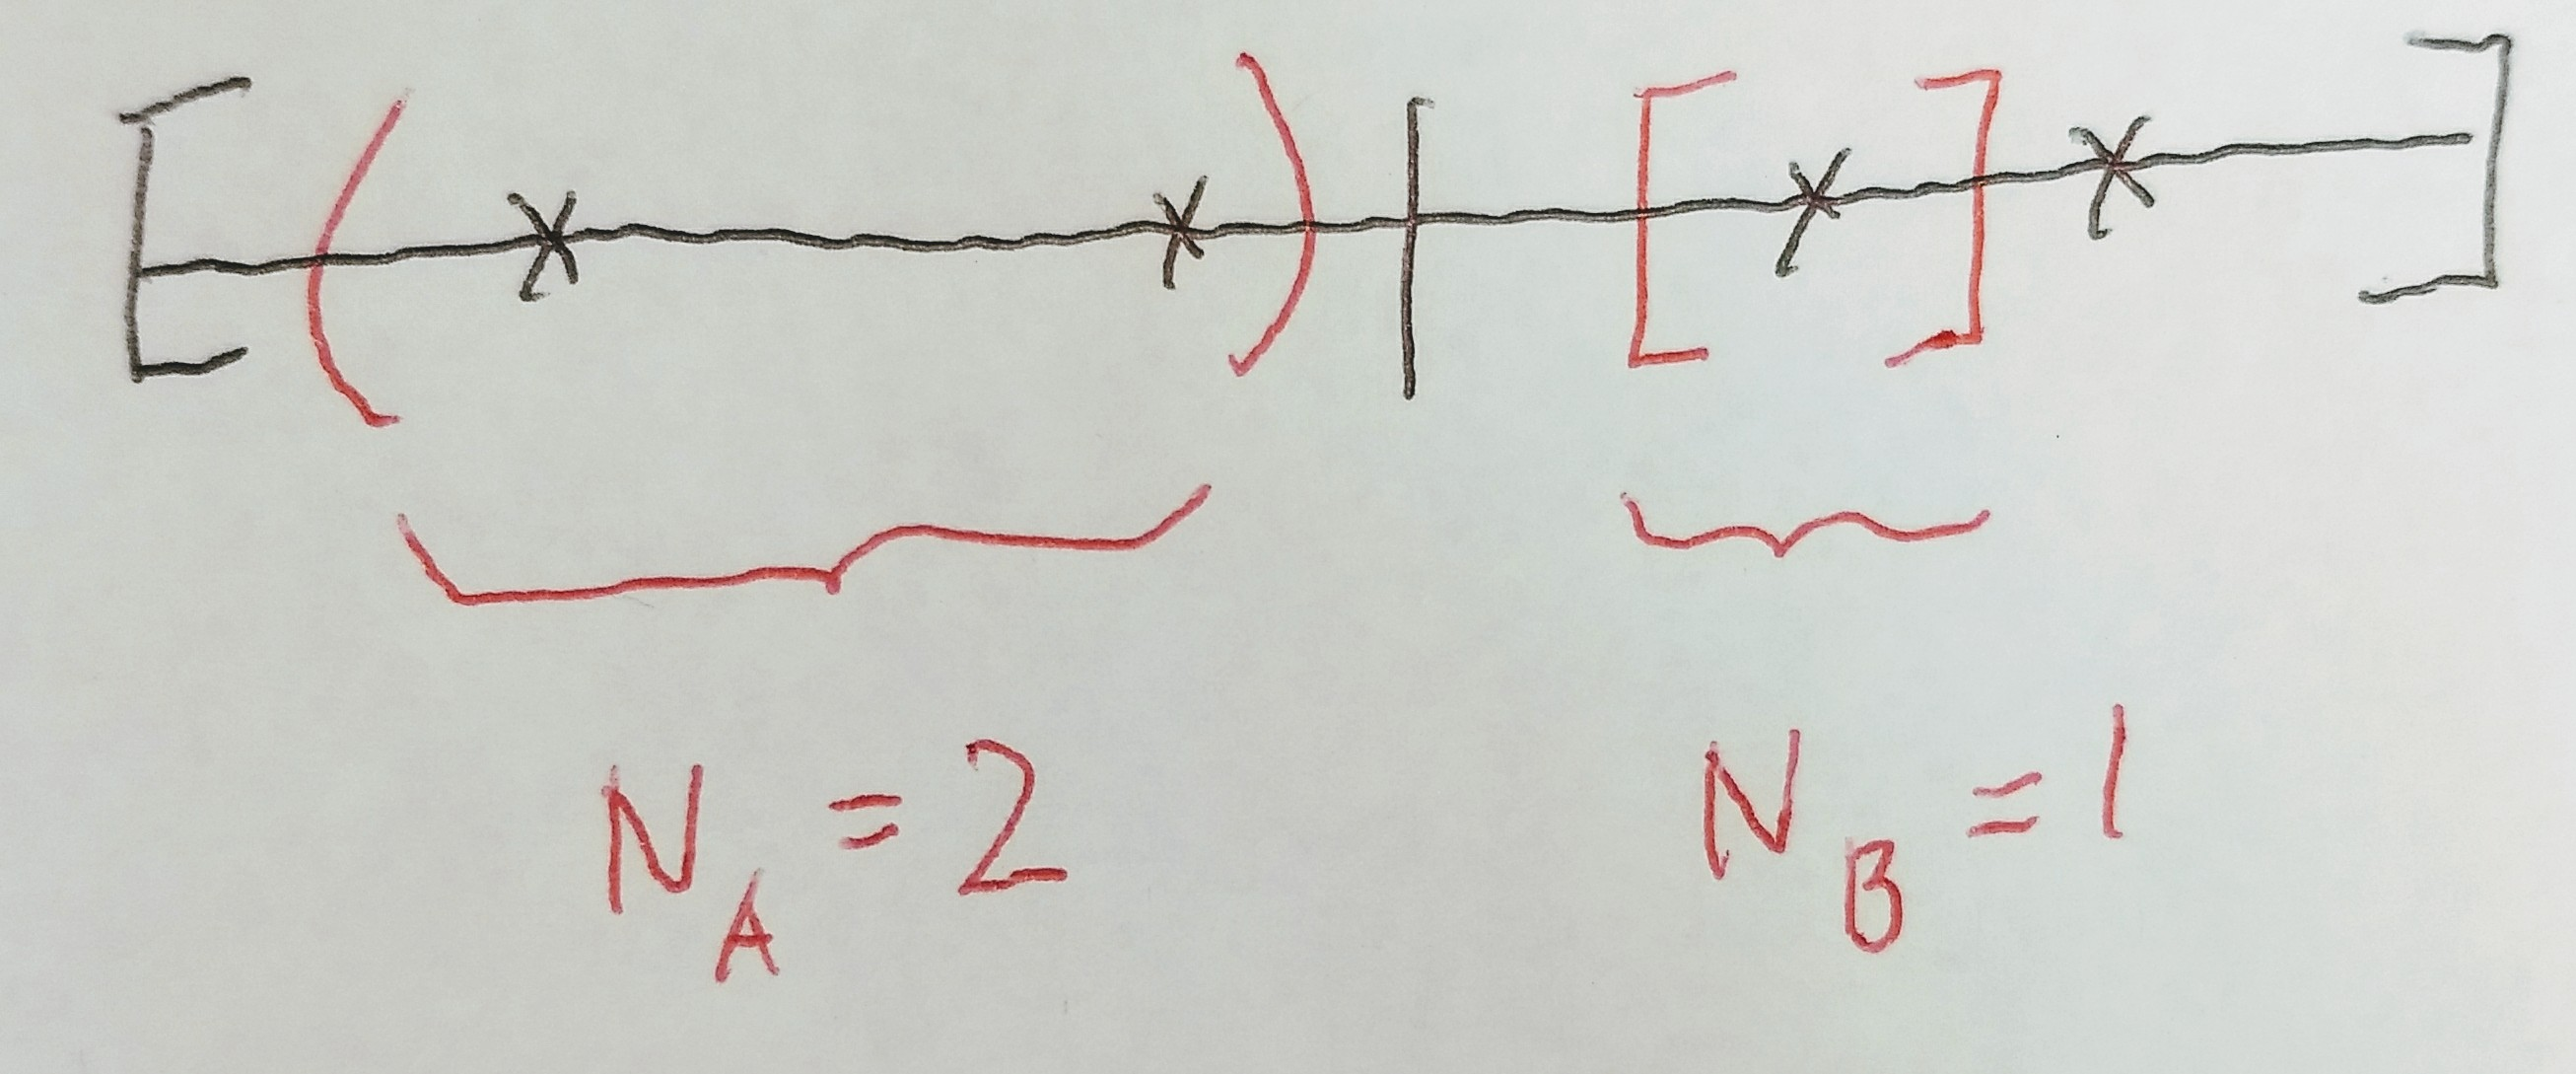
\includegraphics[width=0.5\linewidth]{figures/pp-with-intervals} 
\end{center}

\point{From the motivating example:} we are interested in cases where:
\begin{enumerate}
  \item $A \cap B = \emptyset \Longrightarrow N_A$ and $N_B$ are independent.
  \item $N_A \sim \Poi($length of $A)$. Let us denote the length of $A$ by $\mu(A)$.
\end{enumerate}

\point{Recall:} a nice property of these random variables is:
\[ N_{A\sqcup B} = N_A + N_B \sim \Poi(\underbrace{\mu(A) + \mu(B))}_{\mu(A\sqcup B)} \]

\point{Note:} this is an instance of what is called \emph{Kolmogorov consistency}.

\point{Example 2:} random positions of animals in the forest $\ppspace = [0,1]\times[0,1]$, $\mu = \mu^2$. Exercise: what are the assumptions we implicitly make if we say the animal positions are distributed according to a Poisson process?
\begin{center}
	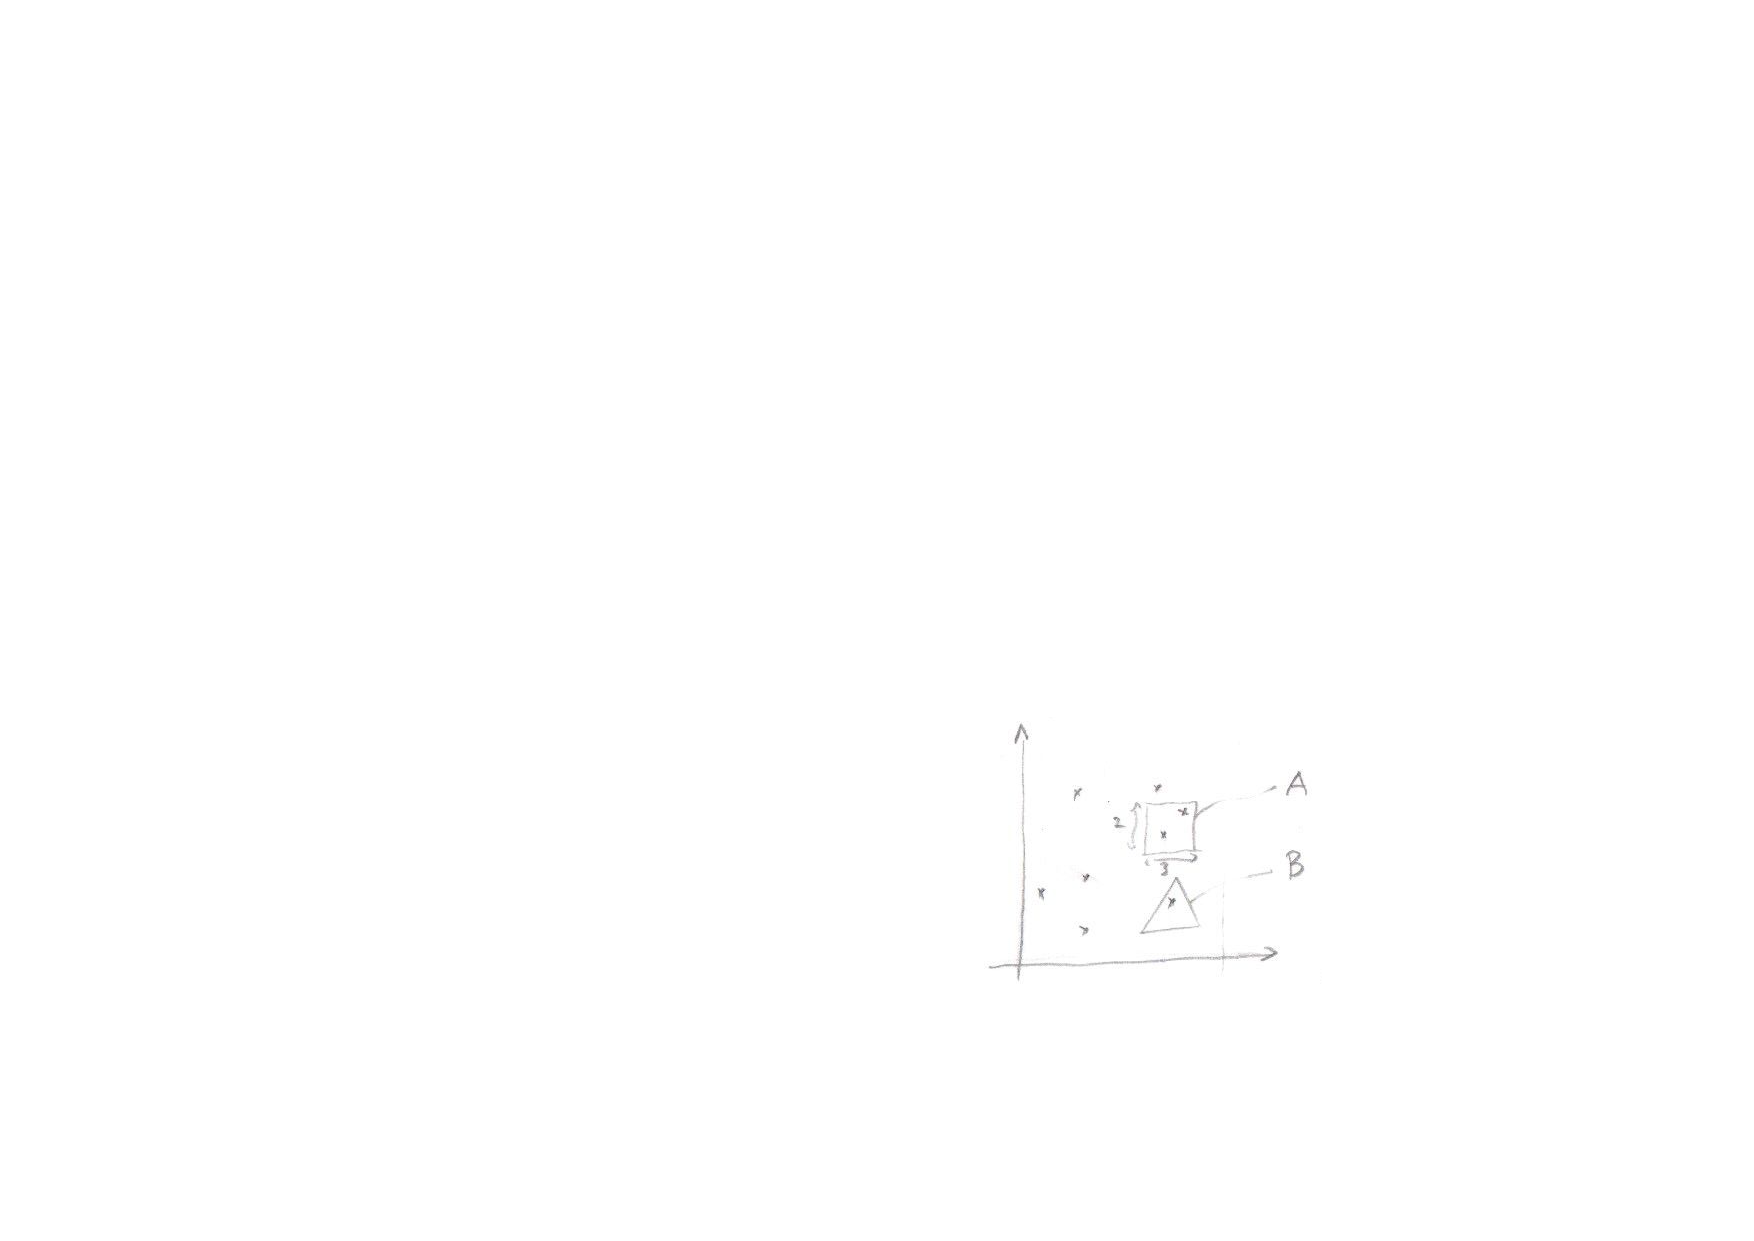
\includegraphics[width=0.5\linewidth]{figures/pp-2d} 
\end{center}
\point{Assumptions in above example:}
\begin{enumerate}
	\item Solitary animals.
	\item Do not avoid each other.
	\item No food/water source attracting animals.
\end{enumerate}
We will next discuss how to relax the last assumption, in the context of another 1d example. 

\point{Example 3:} customers entering a store. Here, $\ppspace = [0, \infty)$ represents time. Problem: same expected number of customers between 1am--2am and 1pm--2pm. Solution? Non-uniform $\mu$, defined via a RN derivative. 
\begin{center}
	\includegraphics[width=0.6\linewidth]{figures/pp-non-unif} 
\end{center}
Compute the intensity via
\[ \mu(A) = \int_A f_\mu(x) \ud x. \]
Then as before,
\[ N_A \sim \Poi(\mu(A)). \]

\point{Next:} a formal definition of Poisson processes. 

\point{Assumptions on} $\mu$, called the intensity measure:
\begin{enumerate}
  \item A measure on $(\ppspace, \events_\ppspace)$,
  \item Can be broken into a countable collection of finite measure segments: exists countable partition $A_i$ of $\ppspace$ such that $\mu(A_i) < \infty$ (this property is called ``$\mu$ is  $\sigma$-finite'').
  \item The intensity measure is non-atomic: for all $x \in \ppspace$, $\mu(\{x\}) = 0$.
\end{enumerate}

\point{Formal definition of a Poisson Process (PP):} under the above assumption, the collection of random variables $\{N_A : A \in \events_\ppspace\}$ is called a Poisson process with intensity $\mu$ if:
\begin{enumerate}
  \item $A \cap B = \emptyset \Longrightarrow N_A$ and $N_B$ are independent.
  \item $N_A \sim \Poi(\mu(A))$.
\end{enumerate}

\point{Constructive definition:}
\begin{enumerate}
  \item Simulate the point for one of the block $A_i$ at the time:
  \begin{enumerate}
    \item Simulate the number of points in $A_i$, $N_{A_i} \sim \Poi(\mu(A_i))$.
    \item For $j = 1, \dots, N_{A_i}$:
    \begin{enumerate}
      \item $X_{i,j}$ is sampled independently according to $\mu$ restricted to $A_i$ and renormalized in order to form a probability distribution, i.e.:
      \[ \P(X_{i,j} \in B) = \frac{\mu(B \cap A_i)}{\mu(A_i)}. \]
    \end{enumerate}
    \item The random set of points in $A_i$ is $S_i = \{X_1, \dots, X_{N_{A_i}}\}$
  \end{enumerate}
  \item Return the union $S$ of the points over all the $S_i$'s
\end{enumerate}
\begin{center}
	\includegraphics[width=0.5\linewidth]{figures/pp-algo} 
\end{center}

\point{Proof sketch:} the distribution of the algorithm satisfies our two defining axioms. 

\point{Lemma:} the distribution of $S$ does not depend on the choice of partition $\{A_i\}$.

\point{Proof of lemma:} consider two partitions $\{A_i\}$ and $\{B_i\}$. We want to show $S_{\{A_i\}} \deq S_{\{B_i\}}$. Build a new partition as we did in exercise~\ref{sec:sol-ex-iii} 
\[ \{ C_{i,j} = A_i \cap B_j \}. \]
Show 
\[ S_{\{A_i\}} \deq S_{\{C_{i,j}\}} \]
and 
\[ S_{\{B_i\}} \deq S_{\{C_{i,j}\}}, \]
where we $S_{\{A_i\}}$ denote the output of the above algorithm using partition $\{A_i\}$.
The key point in the argument is that
\[ N_{A_i} \deq \sum_j N_{C_{i,j}}, \]
which holds by combining additivity of measures
\[ \mu(A_i) \deq \sum_j \mu(C_{i,j}),  \]
and ``additivity'' of Poisson distributions, 
\[ X_i \iidsim \Poi(\lambda_i) \Longrightarrow \sum_i X_i \sim \Poi\left(\sum_i \lambda_i\right). \]

\point{Back to proposition:} given the two set $A$ and $B$ in the axiom, just pick $A_1 = A$ and $A_2 = B$, the proof then follows directly from the lemma.

\point{Counts and sets: two equivalent views.} The algorithm shows that the PP can be viewed as a random set of points, denoted $S \sim \PP(\mu)$. With a slight abuse of notation, if $\mu$ has RN density $f_\mu$, we might also write $S \sim \PP(f_\mu)$.


\subsection{Poisson process with constant intensity on the real line}

\point{Special case:} linking our definition of PP to the undergraduate definition. Assume:
\begin{itemize}
  \item $\ppspace = [0, \infty)$
  \item $\mu =$ uniform.
\end{itemize}
Let $T_1, T_2, \dots$ denote the arrival times, i.e. $T_1 = \inf\{t : N_{[0,t]} \ge 1\}$, and more generally, $T_k = \inf\{t : N_{[0,t]} \ge k\}$.
Then:
\begin{eqnarray}
\P(T_1 > t) &=& \P(N_{[0,t]} = 0) \\
&=& \frac{e^{t - 0} (t-0)^n}{n!} \;\;\text{ with }n=0 \\
&=& 1 - \text{CDF of an exponential}
\end{eqnarray}
Similarly, each inter-arrival times $T_i - T_{i-1}$ are also exponential(1).


\subsection{Superposition}

\point{Motivation:} consider the example concerned with animals in the forest. What if we consider two species simultaneously, assuming they do not interact?

\point{Proposition (superposition):} let $\{S_i\}_{i = 1}^n$ denote a collection of PPs, $S_i \sim \PP(\mu_i)$, where the intensity measures are defined on a common space, $\mu_i : \events_{\ppspace} \to [0, \infty)$. Then $S \defeq \cup_i S_i \sim \PP(\sum_i \mu_i)$.

\point{Exercise:} prove this using the algorithmic construction and the fact that the sum of Poissons is Poisson. 

\point{Note:} this can be generalized to countable unions of PPs, provided that the sum of intensities is still $\sigma$-finite. 


\subsection{Thinning}

\point{Definition (thinning).} Let $S = \{X_1, X_2, \dots\} \sim \PP(\mu)$, $Y_i \iidsim \Bern(p)$. We define the thinned process by using the iid coin flips $Y_i$ to decide, for each point in $S$, whether we keep this point or not: $T \defeq \{X_i \in S : Y_i = 1\}$.

\point{Proposition (thinning).} The random set $T$ defined above by the thinning procedure is a Poisson process, and its intensity is obtained by scaling down the original intensity $\mu$: $T \sim \PP(p\mu)$, where $(p\mu)(A) \defeq p \mu(A)$.

\point{Proof:} will be easier once we talk about conditioning next week. 

\point{Thinning for densities.} Suppose now the intensity measure has a RN derivative, $S = \{X_1, X_2, \dots\} \sim \PP(f_\mu)$. We can let the coin flips be non-identical: given a position of a point $x$, let us say we use for the corresponding $Y$ a coin with success probability $p(x)$ for some $p : \ppspace \to [0, 1]$. Then $T \defeq \{X_i \in S : Y_i = 1\}$ is again a PP, this time with intensity RN given by the pointwise product $f(x) = p(x) f_\mu(x)$.

\point{Powerful computational trick:} let us say you have a complicated intensity function with RN $f$ from which you would like to simulate a PP. If $f$ is bounded by $M$, then you can use the following recipe:
\begin{enumerate}
	\item Let $f_\mu = M$, the uniform density scaled by $M$. Note: $f(x) = p(x) f_\mu(x)$ for some function $p : \ppspace \to [0, 1]$, namely
	\[ p(x) =  \frac{f(x)}{f_\mu(x)} = \frac{f(x)}{M}. \] 
	\item Simulate $S = \{X_1, X_2, \dots\} \sim \PP(f_\mu)$ which is trivial to do.
	\item For each $X_i$, simulate a Bernoulli $Y_i$ with success probability $p(X_i)$.
	\item Return $T \defeq \{X_i \in S : Y_i = 1\}$. By the second thinning theorem, this is distributed according to a PP with intensity $f$ as hoped.
\end{enumerate}
\begin{center}
	\includegraphics[width=0.6\linewidth]{figures/thinning} 
\end{center}

\point{Exercise:} generalize this recipe to $f_\mu(x)$ being some non-constant upper-bound on $f$. 


\subsection{Mapping}

\point{Motivation:} consider the animals in the forest example. What is the distribution of the $x$-coordinates of the random animal locations?

\point{More general setup:} suppose we have a mapping $\phi : \ppspace \to \ppspace'$.
\begin{center}
	\includegraphics[width=0.5\linewidth]{figures/pp-mapping} 
\end{center} 
\point{Exercise:} write the projection example using the framework of a mapping $\phi$.

\point{Solution:} In the above example, $\ppspace = [0,1]^2$, $\ppspace' = [0,1]$, and $\phi(x, y) = x$.

\point{Proposition:} Let $S \sim \PP(\mu)$. Assume $\mu^\star(A) \defeq \mu(\phi^{-1}(A))$ has no atom and is $\sigma$-finite. Then $\phi(S) \sim \PP(\mu^\star)$.


\subsection{Compound PP}

\point{Observation:} let us view the collection of random variable $N_A$ differently, writing it as $N(\cdot)$ instead. What is this? A random measure! Now let us fix a real-valued function $f : \ppspace \to \R$. We can then define the random integral:
\[ Y = \int f \ud N = \sum_{X \in S} f(X). \]

\point{Definition:} $Y$ is called a compound Poisson process.

\point{Next:} we would like to gain information about the distribution of $Y$. We will see that we can compute its characteristic function:
\[ \E\left[e^{itY}\right] = \exp\left\{ \int \left(e^{itf(x)} - 1\right) \mu(\ud x) \right\}. \]

\point{Proof:} start with $f$ simple:
\[ f = \sum_j a_j \delta_{A_j}. \]
Let $\lambda_j = \mu(A_j)$, $N_j \sim \Poi(\lambda_j)$, and
\[ Y = \sum_j a_j N_j. \]
We now compute the characteristic function as follows:
\begin{align*}
\E[ e^{itY} ] &= \prod_j \E[e^{ita_j N_j}] \\
&= \prod_j e^{\lambda_j (e^{ita_j} - 1)} \\
&= \exp\left( \sum_j \lambda_j (e^{it a_j} - 1)\right) \\
&= \exp\left( \int (e^{itf(x)} - 1)\mu(\ud x)\right).
\end{align*}
Next, for arbitrary $f$, use DCT to obtain:
\[ \E[ e^{itY} ] = \exp\left( \int (e^{itf(x)} - 1)		 \mu(\ud x)\right). \]


\section{Conditioning}

\subsection{Background: $\sigma$-algebra and information}\label{sec:sigma-algebra-and-information}

It will be useful for you to review Section~\ref{sec:sigma-alg-and-estimator} before reading this chapter.


\subsection{Conditioning on an event}

\point{Motivation:} a couple has two children. You would like to predict the sex of the second (youngest) child. Your initial beliefs over the sex of that second child is 1/2 boy, 1/2 girl. You get one piece of information: at least one of the two children is a girl. What is the optimal way of updating your beliefs?

\point{Conditioning on an even:} consists in an operator that takes as an input:
\begin{enumerate}
  \item some \emph{a priori} beliefs (a probability distribution $\P(\cdot)$), 
  \item as well as an observed event $E$. 
\end{enumerate}
The interpretation of $E$ is that you know the true outcome is somewhere in $E$, but you still do not know which outcome in $E$. The output of conditioning on an event: a new, updated belief, denoted $\P(\cdot | E)$. The optimal value for this updated belief, for any query set $A$, is given by:
\[ \P(A | E) = \frac{\P(A\cap E)}{\P(E)}. \]

\point{Example.} In the motivation at the beginning of the section, we are interested in $A$ and $A^\complement$, where $A = \{(g,g), (b,g)\}$. The observation is $E = \{(b,g),(g,b),(g,g)\}$, hence the updated belief for the motivation question is $\P(A|E) = 2/3, \P(A^\complement|E) = 1/3$.


\subsection{Conditioning on a random variable}

\point{Interpretation:} let $X$ and $Y$ be two random variables defined on the same probability space:
\begin{itemize}
  \item $Y$ is observed, (e.g. $Y = \1_E$ in the motivating example)
  \item $X$ is the variable you would like to predict (e.g. $X = \1_A$ in the motivating example).
\end{itemize}
The conditional expectation of $X$ given $Y$ is a new estimator random variable $\delta = f(Y)$, which can be interpreted as the ``best'' estimator of $X$ based on $Y$. Notation: this random variable $\delta$ is denote by $\E[X|Y]$.

\point{Notion of optimality:} consider the optimization program
\[ \text{minimize}\ \E(f(Y) - X)^2, \]
where minimization is performed over functions $f$ (technically, over measurable functions). If a function $f^*$ maximizes this program and give a finite value to the objective function, then $\E[X|Y] \defeq f^*(Y)$.

\point{Exercise:} show that in the two children problem, you obtain:
\[ f^*(y) = \bracearraycond{0 \;\;&\text{if }y=0\\ 2/3\;\;&\text{if }y=1\\\text{any value}\;\;&\text{otherwise.}} \] 

\point{Solution:} we have:
\begin{align*} \E(f(Y) - X)^2 &= \frac{1}{4}\left[ (f(0) - 0)^2 + (f(1) - 1)^2 + (f(1) - 0)^2 + (f(1) - 1)^2 \right] \\ 
&= \frac{f(0)^2 + 3 f(1)^2 - 4f(1) +2}{4},
\end{align*}
hence we see right away that $f(0) = 0$ and that the values of $f$ are unimportant except at $y=0$ and $y=1$. To find $f_1 = f(1)$, we compute the derivative with respect to $f_1$ and get
\[ \frac{\ud}{\ud f_1} \left(  \frac{3 f_1^2 - 4 f_1 +2}{4}\right) = \frac{3}{2} f_1 - 1, \]
hence finding the root we get indeed $f_1 = 2/3$.

\point{Note:} by the discussion in Section~\ref{sec:sigma-algebra-and-information}, note that we only used $Y$ via $\sigma(Y)$. For this reason, we can define the notion of conditioning on a $\sigma$-algebra $\events$, denoted $\E[X|\events]$, in the same way as we did above.

\point{Notation:} $\|X\|_2 \defeq \sqrt{\E[X^2]}$, $\L_2 \defeq \{\text{r.v. } X : \|X\|_2 < \infty\}$.

\point{Note:} we will see that the above definition always works when $Y \in \L_2$. To generalize this to $Y \in \L_1$, we will make use of a generalization of a property which is itself very important in practice: the law of total expectation.


\subsection{The law of total probability and expectation}

\point{Useful property:} the law of total expectation:
\[ \E[X] = \E[\E[X|Y]], \]
and its associated law of total probability, a special case where $X = \1_A$:
\[ \P(X \in A) = \E[ \P(X \in A|Y) ]. \]

\point{Example/exercise:} suppose that
\begin{eqnarray*}
U &\sim \Unif(0,1) \\
X | U &\sim \Bin(n, U),
\end{eqnarray*}
Show that $\P(X = i) = 1/(n+1)$ using the law of total probability. Hint: use the Beta function, defined for $x> 0$ and $y > 0$:
\[ B(x, y) = \int_0^1 u^{x-1} (1-u)^{y-1} \ud u = \frac{\Gamma(x) \Gamma(y)}{\Gamma(x+y)}, \]
where $\Gamma$ denotes the Gamma function, which for integer $x$ satisfies $\Gamma(x) = (x-1)!$.

\point{Notation used above:} what do we need precisely by ``$X | U \sim \Bin(n, U)$''? More generally, suppose $\{D_y\}$ is some collection of distribution indexed by a parameter $y$ (e.g. the Binomials indexed by their success probability parameter). Then the notation ``$X|Y\sim D(Y)$'' means that for all $A$, $\P(X\in A|Y) = D_Y(A)$.

\point{Solution:} by the Law of Total Probability, $\P(X=i) = \E[ \P(X=i | U) ]$. By the distributional statement $X|U \sim \Bin(n, U)$, and the fact that the Binomial distribution has a known probability mass function in which we plug in (compose) with the random success probability parameter $U$:
\begin{align*}
	\P(X = i) &= \E[ \P(X=i | U)] \\
	&= \E\left[ \binom{n}{i} U^i (1 - U)^{n-i} \right] \\
	&= \binom{n}{i} \E\left[ U^i (1-U)^{n-i} \right].
\end{align*}
Now the last line is the expectation of a function $g(u) = u^i (1-u)^{n-i}$ of a uniform random variable. Therefore we can compute as:
\begin{align*}
	\P(X = i) &= \binom{n}{i} \E\left[ U^i (1-U)^{n-i} \right] \\
	&= \binom{n}{i} B(i+1, n - i + 1) \\
	&= \frac{1}{n+1},
\end{align*}
using the hint.

\point{Discrete case:} to get more intuition on the law of total expectation/probability, let us first assume that $Y$ is simple, $Y = \sum_{i=1}^n a_i \1_{A_i}$, where $A_i$ forms a partition. By simple set properties:
\begin{eqnarray*}
\P(A) &=& \sum_{i=1}^n \P(A \cap (Y=a_i)) \\
&=& \sum_{i=1}^n \P(A|Y=a_i) \P(Y = a_i).
\end{eqnarray*}
Now, let: 
\begin{equation} 
f(y) = \bracearraycond{
  \P(A|Y=y) &\text{if }y\in\{a_1, \dots, a_n\} \\ 
  \text{arbitrary,} & \text{otherwise.}
}
\end{equation}
Conditioning on a random variable can be thought as introducing a nice notation for this identity, $\P(A|Y) := f(Y)$. This also provides a way to generalize to conditioning into a non-discrete random variable.

\point{Next:} we first generalize the above to cases where we select only a subset of the blocks in the partition. To formalize this, let $B \subset \{a_1, \dots, a_n\}$, then a set of blocks can be denoted as $H \defeq (Y \in B)$, i.e. $H \in \sigma(Y)$. With this notation, show that:
\[ \P(A \cap H) = \E[ \1_H \P(A | Y)]. \]
\begin{center}
	\includegraphics[width=0.6\linewidth]{figures/law-of-total-pr} 
\end{center}

\point{Definition of conditional probability:} we will use this property, which we have shown to hold for simple $Y$, as the basis of our fully general definition of conditional probability.  Let $Y \in \L_1$. Then there exists a random variable, denoted $\P(A|Y)$, such that:
\begin{enumerate}
  \item $\P(A|Y) \in \sigma(Y)$, (i.e. $\P(A|Y)$ is an estimator based only on the information offered by $Y$)
  \item for all $H \in \sigma(Y)$, $\P(A \cap H) = \E[ \1_H \P(A | Y)]$.
\end{enumerate} 
Moreover this random variable is almost sure unique.

\newcommand\othersigma{{\mathcal G}}

\point{Ingredient for the proof: Radon-Lebesgue-Nikodym theorem} let $(\Omega, \othersigma)$ denote a measurable space with two measures $\nu$ and $\mu$. Then $\mu(A) = 0 \Rightarrow \nu(A) = 0$ (a property called ``$\nu$ is absolutely continuous with respect to $\mu$'', denoted $\nu \ll \mu$), if and only if $\nu$ has a density with respect to $\mu$, i.e. $\nu(A) = \int_A f \ud \nu$ for some $f \in \othersigma$.

\point{Proof of existence of conditional expectation:} let $\othersigma = \sigma(Y)$, and define, for all $H \in \othersigma$, $\nu(H) = \P(A \cap H)$ and $\mu(H) = \P(H)$. Since $\mu(H) = 0 \Longrightarrow \nu(H) = 0$, it follows by Radon-Lebesgue-Nikodym that there is a $f \in \othersigma$ such that $\nu(H) = \int_H f \ud \mu$. This yields the result with $f = \P(A|Y)$. 

\point{Proof of uniqueness:} suppose there are two random variables $Z_1 = \P(A|Y)$ and another one $Z_2$ both satisfying the two conditions in the definition of conditional probability. We have $\E[\1_H Z_1] = \P(A\cap H) = \E[\1_H Z_2]$, therefore $\E[\1_H (Z_1 - Z_2)] = 0$ for all $H \in \sigma(Y)$. Take $H = (D > 0)$, we get by Chebyshev, $\E[\1_H D] = 0 \Longrightarrow \P(D > 0) = 0$. By a symmetrical argument on $Z_2 - Z_1$, $\P(D < 0) = 0$.

\point{Definition of conditional expectation:} a generalization of the above yield also the definition conditional expectation.  Let $X, Y \in \L_1$ be defined on a common probability space. Then there exists a random variable, denoted $\E[X|Y]$, such that:
\begin{enumerate}
\item $\E[X|Y] \in \sigma(Y)$, (i.e. $\E[X|Y]$ is an estimator of $X$ based on $Y$)
\item for all $H \in \sigma(Y)$, $\E[ \1_H X ] = \E[ \1_H \E[X|Y] ]$.
\end{enumerate} 
Moreover this random variable is almost sure unique.


\subsection{Key properties}

\point{Important exercise:} suppose $(X, Y)$ have joint density $f(x,y)$. Then $\E[X|Y] = \psi(Y)$, where 
\begin{eqnarray*} 
\psi(y) &\defeq& \bracearraycond{\int x f_{X|Y}(x|y) \ud x &\text{if }f_Y(y) > 0 \\ \text{arbitrarily,} &\text{otherwise,}} \\
 f_{X|Y}(\cdot|y) &\propto& f(\cdot, y) \\
&\defeq& \frac{f(\cdot,y)}{f_Y(y)} \\
f_Y(y) &\defeq& \int f(x, y) \ud x.
\end{eqnarray*}

\point{Terminology:} the function $f_Y(\cdot)$ is called the marginal density, and the function $f_{X|Y}(\cdot|y)$, the conditional density. Note that these are indeed densities. 

\point{Property:} when $X,g(Y) \in \L_1$, \[ \E[ X g(Y) | Y] = g(Y) \E[X|Y]. \]

\point{Proof:} we have to show that the RHS satisfies the two axioms of conditional expectation. For (1), clearly it is of the form $f(Y)$. For (2), let $H \in \sigma(Y)$, and suppose first that $g(y) = \1_B$, implying that $g(Y) = \1_G$, $G \in \sigma(Y)$. We get:
\begin{eqnarray*}
\E[ \1_H X \1_G ] &=& \E[ \1_H \1_G \E[X|Y] ] \Leftrightarrow \\
\E[ \1_{H'} X ] &=& \E[ \1_{H'} \E[X|Y] ],
\end{eqnarray*}
which is true since $H' \in \sigma(Y)$. Complete the proof using the DCT.
\begin{center}
	\includegraphics[width=0.6\linewidth]{figures/cond-exp-property} 
\end{center}


\subsection{Equivalence of the two definitions}

So far, we have given two definitions of conditional expectations, one that works for $\L_2$ only, and one that works for $\L_1$ and $\L_2$. Here we show that for the $\L_2$ setup, our new, general definition agrees with the $\L_2$ specific earlier definition:
\begin{eqnarray*}
\E[ (f(Y) - X)^2 ] &=& \E[ \E[ (f(Y) - X)^2 | Y ]] \\
&=& \E [ \underbrace{ \E[ f(Y)^2 | Y ]}_{(f(Y))^2} - \underbrace{ 2 \E[ f(Y) X | Y] }_{2 f(Y) \E[X|Y]} + \E[ X^2 | Y] ] \\
&=& \E[ \underbrace{(f(Y) - \E[X|Y])^2}_{\ge 0} + \underbrace{ \E[X^2 | Y] - (\E[X|Y])^2 }_{\defeq \var[X|Y]} ].
\end{eqnarray*}
Note:
\begin{enumerate}
  \item the RHS$\ge \E[ \var[X|Y]]$.
  \item if $f(Y) = \E[X|Y]$ a.s., then RHS$=\E[\var[X|Y]]$.
\end{enumerate}


\subsection{The Bayes estimator (a special case)}

\point{Motivation:} a complete order over estimator. 

\point{Frequentist notion of optimality:} since in the MLE (Maximum Likelihood Estimation) framework we do not place a prior on $\theta = X$, the performance of an estimator $\delta$ depends on the true parameter $\theta$:
\[ \text{MSE}_\theta(\delta) = \E_\theta[(\delta - \theta)^2] = \E[(\delta - \theta)^2 | \theta]. \]
The MLE mimizes this objective function.

\point{Issue:} the space of functions (of $\theta$ in this case) is not a complete order. There is not a notion of an a.s. best estimator under the above criterion.

\point{Solution:} restrict the class of estimators, e.g. to unbiased ones.

\point{Criticism:} can be restrictive/artificially rule out good estimators. 

\point{Bayesian alternative:} average over $\theta$, to get a real number summary of each estimator:
\[ \text{mse}(\delta) = \E[ \text{MSE}_\theta(\delta) ]. \]

\point{Consequence:} this yields a \emph{complete order} over estimator. The name of the best estimator is called the \emph{Bayes estimator}, and corresponds to the posterior mean $\E[\theta | \text{data}]$ with our choice of loss function being the square difference. 

\point{Note:} the Bayes estimator can be defined for other loss functions, in which case it involves an optimization problem where the objective function is a conditional expectation given the data.


\subsection{Geometric view of expectation and further properties}

Suppose in the remaining of the section that $Y \in \L_2$. 

\point{Recall:}
\begin{itemize}
  \item Real vector space: a set $V$ of points in $\R^d$ and a $+$ and $\cdot$ operations such that a set of useful properties hold (associativity, $v_1 + (v_2 + v_3) = (v_1 + v_2) + v_3$, distributivity $a(v_1 + v_2) = a v_1 + a v_2$, etc (see wikipedia)).
  \item Abstract vector space: a set of objects $V$ with two operations satisfying the same properties.
\end{itemize}

\point{Example:} $V = \L_2 = \{\text{r.v. }X: \Omega \to \R, \E X^2 < \infty\}$. Easy exercise: read the axioms on wikipedia and check they are satisfied with $+$ denoting the addition of functions and $\cdot$, the multiplication of a function by a constant.

\point{Three important ideas from linear algebra.}

\point{1. Norm:} $\|\cdot\| : V \to [0, \infty)$. Key defining property (see wiki for the other ones): $\|v + w\| \le \|v\| + \|w\|$ (triangle inequality).

\point{Examples:}
\begin{enumerate}
  \item $V = \R^2$, $\|v\|_2 = \sqrt{v_1^2 + v_2^2}$, triangle inequality is the Pythagorean theorem.
  \item $V = \L_2$, $\|X\| = \sqrt{\E X^2 }$, triangle inequality is called Minkowski's inequality, described in more detail shortly.
\end{enumerate}

\point{2. Subspace:} a ``closed'' subset of a vector space, $W \subset V$, i.e. such that $v_1, v_2 \in W \Rightarrow v_1 + v_2 \in W$. 

\point{Examples:}
\begin{enumerate}
  \item $\{$points of the form $(0, x)\} \subset \R^2$,
  \item $W = \{Z \in \L_2 : Z \in \sigma(Y)\} = \{Z \in \L_2 : Z = f(Y), f\text{ measurable}\}$. 
\end{enumerate}

\point{3. Projection:} of a point $v$ into a subspace $W$. This projection is defined as:
\[ \argmin_{w \in W} \| v - w\|. \]

\point{Key example:} when $V = \L_2$, $W$ as point 2 above:
\begin{eqnarray*}
\E[X|Y] &=& \argmin_{Z \in W} \| Z - X \| \\
&=& \text{projection of $X$ into $W$.}
\end{eqnarray*}

\point{Application:} if $\events_1 \subset \events_2$, then:
\begin{eqnarray*}
\E[\E[X|\events_1]|\events_2] &=& \E[\E[X|\events_2]|\events_1] \\
&=& \E[X | \events_1].
\end{eqnarray*}

\point{Proof sketch:} 
\begin{center}
	\includegraphics[width=0.6\linewidth]{figures/tower} 
\end{center}


\point{Last few properties of conditional expectations:}
\begin{enumerate}
  \item Linearity: $\E[a X + Y|\events] = a \E[X|\events] + \E[Y|\events]$.
  \item Monotonicity.
  \item Jensen's inequality.
  \item Chebyshev.
\end{enumerate}


\subsection{Geometric view: more details on triangle inequality}

\point{Minkowski inequality:} is usually proven using \emph{Cauchy-Schwarz inequality}, which is a must-know itself.

\point{Cauchy-Schwarz:} $|\dotprod{u}{v}| \le \| u \|_2 \| v \|_2$, where $\dotprod{\cdot}{\cdot}$ denotes an inner product, e.g. $\dotprod{X}{Y} = \E[X Y]$. This result should be pretty intuitive: suppose you have two vectors $u$ and $v$ of fixed length and you want to maximize their dot product. How to do this? Make them point in the same direction! In this case we actually get equality. In the case of a real vector space, this is clear from the identity $\dotprod{u}{v}^2 = (\| u \|_2 \| v \|_2 \cos \theta)^2 \le (\| u \|_2 \| v \|_2)^2$, where $\theta$ is the angle between the two vectors. See wikipedia for the general proof.

%The proof follows from a generalization of the fact that $(a - b)^2 \ge 0$ hence $2ab \le a^2 + b^2$.

\point{Minkowski from Cauchy-Schwarz:} 
\begin{align*}
\| X + Y \|_2^2 &= \E | X + Y |^2 \\
&\le \E [ (|X| + |Y|) |X + Y| ] \\
&= \E [ |X|\times|X + Y| ] + \E [ |Y|\times|X + Y| ] \\
&\le \| X \|_2 \|X + Y\|_2 + \| Y \|_2 \|X + Y\|_2 \;\text{ (using Cauchy-Schwarz)}  \\
&= ( \| X \|_2 + \| Y \|_2 ) \|X + Y\|_2.
\end{align*} 
Finally, divide each side by $\|X + Y\|_2$.

\point{Generalizations:} to go from $L^2$ to $L^p$, $p \ge 1$ is easy. Search \emph{H\"{o}lder's inequality} and use that instead of Cauchy-Schwarz in the above argument. 


\subsection{Conditional independence}

\newcommand\independent{\protect\mathpalette{\protect\independenT}{\perp}}
\def\independenT#1#2{\mathrel{\rlap{$#1#2$}\mkern2mu{#1#2}}}

\point{Conditional independence of events:} events $A$ and $B$ are conditionally independent given $C$, denoted $A \independent B | C$, if \[\P(A \cap B | C) = P(A | C) P(B | C).\] Notice this is just the standard  notion of independence applied to a conditional probability $\P(\cdot | C)$.

\point{Conditional independence of random variables:} two random variables $X$ and $Y$ are conditionally independent given $Z$, $X \independent Y | Z$, if \[ \E[g_1(X) g_2(Y)|Z] = \E[g_1(X)|Z] \E[g_2(Y)|Z]\] for all bounded continuous $g_1, g_2$.

\point{Exercise:} independence does not imply conditional independence, and conditional independence does not imply independence. Hint: consider the following 
\begin{enumerate}
	\item The random variables $X_1, X_2, X_3$ corresponding to the position of a player of ladders and snakes at turns one, two and three (ignore the snakes and ladders for simplicity), $X_1 \sim \Unif(1, \dots, 6)$, $X_i | X_{i-1} \sim \Unif(X_{i-1} + 1, \dots, X_{i-1} + 6)$.
	\item The random variable $S = Y_1 + Y_2$ where $Y_1$ and $Y_2$ correspond to the throwing of two dice. 
\end{enumerate}


\subsection{Directed graphical models}

\point{Generative model:} a description of a joint distribution as a product of conditional distribution. By the chain rule, this can always be done, but typically we expect a generative model to be such that each conditional distribution can be efficiently simulated from. 

\point{Example:} (made up)
\begin{align*}
	X_1 &\sim \Unif(0, 1/2, 1) \\
	X_2 | X_1 &\sim \Bern(X_1) \\
	X_3 | X_1, X_4 &\sim \Poi(1 + X_1 + X_4) \\
	X_4 &\sim \Bern(1/3) \\
	X_5 | X_3 &\sim \Unif(0, .., X_3) \\
	X_7 &\sim \text{Geo}(1/4) \\
	X_6 | X_4, X_7 &\sim \Unif(X_4, X_7) \\
	X_8 &\sim \text{Norm}(0, 1) 
\end{align*}

\point{Motivation for directed graphical models:} they help us address the following two problems:
\begin{enumerate}
	\item Design an algorithm to sample from the joint distribution $f(x_1, x_2, \dots, x_8)$.
	\item Efficiently establish some conditional independence relationships. For example, do we have $X_4 \independent X_2 | X_1, X_5, X_6$? We will cover this in the next section.
\end{enumerate}

\point{First problem: sampling from the joint distribution.} This task arises when you need to generate ``synthetic data'' in a Bayesian context. This is also called ``forward sampling.'' The basic problem is that if there are $n$ variables, the chain rule can be written in $n!$ ways. Which one to pick? E.g.: compare these three orders
\begin{enumerate}
	\item $f(x_1, x_2, \dots, x_8) = f(x_1) f(x_2 | x_1) f(x_3 | x_1, x_2) f(x_4 | x_1, x_2, x_3) \dots f(x_8 | x_1, \dots, x_7)$, and order we denote by $(1,2,3,4,5,6,7,8)$,
	\item order $(1, 4, 7, 2, 3, 6, 5, 8)$,
	\item order $(8, 1, 2, 4, 3, 5, 7, 6)$.
\end{enumerate}
It is much easier to simulate from order 2 than order 1. Why? At the same time, order 2 is not unique: 3 would be just as efficient. Directed graphical models will bring much clarity here:

\point{Definition:} a directed graphical model is a directed model where nodes are variables and there is an edge from variable $X_i$ to $X_j$ if the conditional distribution of $X_j$ in the generative model depends on $X_i$. 

\point{Example.} For the previous generative model, we obtain:
\begin{center}
	\includegraphics[width=0.5\linewidth]{figures/graph-model} 
\end{center}

\point{Forward sampling using graphical models:} pick an order $(i_1, i_2, \dots)$ such that the edges of the graphical model are respected, i.e. for all edge $(i_k \to i_l)$, the first end point appear earlier in the order compared to the second, $k < l$. This is called a \emph{linearization} of a partial order, and can be performed in linear time in the size of the graph, via an algorithm called \emph{topological sorting}.


\subsection{Establishing (conditional) independence relations using directed graphical models}

\point{Establishing certain independence relations.} Let us start with independence, and do conditional independence after. 

\point{Idea:} We can sometimes infer independence relationships just by looking at the shape of the graphical model.

\point{Example:} using the same graphical model as before, suppose we want to find if $X_4$ is independent of $X_7$.

\point{Bayes ball algorithm for independence.} The rules of this algorithm are as follows:
\begin{enumerate}
	\item Two nodes \emph{communicate} if there is some path following the graphical rules below. In this case we \emph{cannot say} just from the graphical model if the random variables are independent
	\item If there are no such path, the nodes do not communicate. In this case we can conclude the random variables are independent
\end{enumerate}
\begin{center}
	\includegraphics[width=0.2\linewidth]{figures/rules-unconditioned} 
\end{center}

\point{Exercise:} In our usual example, which nodes are guaranteed to be independent of $X_4$?

\point{Solution:} $X_1, X_2, X_7, X_8$.

\point{Conditional independence.} Suppose now we want to find conditional independence statements. We first extend our notion of graphical model:

\point{Convention:} shade in grey the random variables that we want to condition upon.

\point{Example.} In our recurring model, let us condition on $X_1, X_5, X_6$.
\begin{center}
	\includegraphics[width=0.5\linewidth]{figures/graph-model-cond} 
\end{center}

\point{Bayes ball algorithm for independence.} The algorithm works in the same way but with the following extended rule set taking into account shaded nodes:
\begin{center}
	\includegraphics[width=0.4\linewidth]{figures/bayes-ball-full-rules} 
\end{center}

\point{Example:} From the usual graphical model, which of the white nodes\footnote{Shaded nodes are always conditionally independent, since, for any events $A$, $B$, $C$: $\P(AB|BC) = \P(A|BC)\P(B|BC) = \P(A|BC)$.} are guaranteed to be conditionally independent of $X_4$ given the shaded nodes?

\point{Solution:} $X_2$ and $X_8$.


\section{Markov chains}

\subsection{Basic definitions and examples}

\point{Informal:} A sequence of random variables where the future is independent of the past given the present. 

\point{From the graphical model point of view:} a chain-shaped graphical model.

\point{Formal:} a sequence of random variables $X_i : \Omega \to \states$ is Markov if for all $A \in \events_\states$, 
\[ P(X_{n+1} \in A | X_0, X_1, \dots, X_n) = \P(X_{n+1} \in A | X_n). \]

\point{Examples:}
\begin{enumerate}
  \item Let $E$ denote a set of undirected edges over $\states$. Define \[ \P(X_{n+1} = x | X_n) = \frac{1}{Z(X_n)} \1[\{x, X_n\} \in E]. \]Note that the normalization $Z(x)$ is given by the number of nodes connected to $x$. For example $Z(\text{f}) = 3$ below: 
  \begin{center}
  	\includegraphics[width=0.3\linewidth]{figures/discrete-graph} 
  \end{center}
  To make this more interesting, consider the vertices of the graph given by the location of a knight on a game of chess (8x8 square), and the edges given by the moves allowed for the knight (L shaped moves moving by one square in one axis, and 2 in the other axis). 
  \item The Wright-Fisher model: suppose that $N$ bacteria can live in a Petri dish. There are two species, blue and green bacteria. In the first day, there are $X_1$ green and $N-X_1$ blue bacteria. In the next day, there are still $N$ bacteria, the descendants from the previous generation. The parent of each of the $N$ in day 2 are selected independently and uniformaly from those in day 1. The color is inherited without mutation. This mean: \[ \P(X_n = k | X_n) = \binom{N}{k} \left(\frac{X_n}{N}\right)^k \left( 1 - \frac{X_n}{N}\right)^{N-k}. \]Note that $X_n = 0 \Rightarrow X_{n+1} = 0$, and $X_n = N \Rightarrow X_{n+1} = N$. These are called absorbing states.  
\end{enumerate}


\subsection{Representation under the homogeneity condition}

\point{Note:} from the previous part on conditioning, we have that $\P(X_{n+1} = y | X_n) = f(X_n)$ for some $f(x)$. In fact, this function will also depend on $y$ and $n$. We denote it by $p_n(x \to y)$ and call it the transition probability.

\point{Definition:} a Markov chain is homogeneous is $p_n(x \to y) = p_{n+1}(x \to y)$ for all $n, x, y$. We denote it by $p(x \to y)$. 

\point{Visualization:} of $p(x \to y)$ via a \emph{state diagram}. Consider a directed graph where the nodes are the points in $\states$ and where the is an edge $(x \to y) \in E$ if and only if $p(x \to y) > 0$. Informally, this encodes the sparsity patterns of the transition probabilities.
\begin{center}
	\includegraphics[width=0.3\linewidth]{figures/state-diagram} 
\end{center}

\point{Note:} if $X_n$ is finite and homogeneous, it is characterized by 2 objects:
\begin{enumerate}
  \item the transition probabilities, $p = p_n$,
  \item an initial distribution with pmf $\mu$, $\P(X = x) = \mu(x)$. 
\end{enumerate} 

\point{Notation:} it is often useful to have the initial distribution put all the mass on a single point $x$, in which case we write $\P_x$. E.g. $\P_x(X_1 = y) = p(x \to y)$. 


\subsection{First connection with linear algebra: Chapman-Kolmogorov equation}

\point{Matrix notation for transition probabilities:} to create connections with linear algebra, it will be useful to organize the transition probabilities into a matrix (assuming without loss of generality that $\states = \{1, 2, \dots, K\}$): $M_{x,y} = p(x \to y)$.

\point{Vector notation for pmfs over the states:} if $\mu$ is a pmf over $\states$ (for example, an initial distribution), we can view it as a vector, $\mu = (\mu(1), \mu(2), \dots, \mu(K))$. 

\point{How to find the 2-step transition,} i.e. $\P(X_{n+2} = y | X_n = x)$? As usual we reintroduce the random variable $X_{n+1}$ using marginalization/the law of total probability:
\begin{eqnarray*}
\P(X_{n+2} = y | X_n = x) &=& \sum_{z \in \states} \P(X_{n+2} = y, X_{n+1} = z | X_n = x) \\
&=& \sum_{z \in \states} \P(X_{n+1} = z | X_n = x) \P(X_{n+2} = y | X_n = x, X_{n+1} = z) \;\;(\text{chain rule}) \\
&=& \sum_{z \in \states} \P(X_{n+1} = z | X_n = x) \P(X_{n+2} = y | X_{n+1} = z) \;\;(\text{Markov assumption}) \\
&=& \sum_{z \in \states} p(x \to z) p(z \to y) \\
&=& (M^2)_{x,y}.
\end{eqnarray*} 
\begin{center}
	\includegraphics[width=0.4\linewidth]{figures/kolm-chap} 
\end{center}

\point{Exercise:} show that more generally, \[\mu M^n = (\P(X_n = 1), \P(X_n = 2), \dots, \P(X_n = K)).\]


\subsection{Hitting probabilities}

\point{Setup:} suppose we have an homogeneous finite state Markov chain $X_n$ with exactly two absorbing states, denoted $x_1$ and $x_2$.

\point{Example/exercise:} create a state space to model two-players snakes and ladders. The interpretation of $x_0$ is that the first player wins, and $x_1$, that the second player wins. 

\point{Definition:} a hitting time $T_x$ is the first time (possibly infinity) that a state $x$ is reached, i.e. $T_x = \inf \{n : X_n = x\}$. 

\point{Idea:} solve a bigger problem! What are the hitting probability \emph{for all starting points}, i.e. computing $h(x) = \P_x(T_{x_1} < T_{x_2})$. This allows us to build a recurrence between these problems.

\point{Some easily obtained constraints on $h$:}
\begin{enumerate}
  \item $h(x_1) = 1$ and $h(x_2) = 0$.
  \item $0 \le h \le 1$.
  \item Exercise (using an argument similar to the one used for the Chapman-Kolmogorov equation): \[ h(x) = \sum_{y\in\states} p(x\to y) h(y). \]
\end{enumerate}

\point{Main result:} these constraints can be used to find the numerical value of $h(x)$. More precisely, $h(x)$ is the minimum function satisfying the above three conditions.


\subsection{Asymptotic behavior: overview}

\point{Assumptions:} In the following, we will:
\begin{itemize}
  \item always assume homogeneity,
  \item start by assuming finite $\states$, then relax later on.
\end{itemize}

We will cover two main results, used in different contexts:
\begin{enumerate}
  \item The law of large number for Markov chains. Informally, that sums converge to a constant: \[ \frac{1}{N} \sum_{n=1}^N f(X_n) \ascv c,\]where this constant is obtained by an expectation, $c = \E[f(X_\infty)]$, and $\pi(x) = \P(X_\infty = x)$ is called the stationary distribution. This is used for example in the context of Markov chain Monte Carlo (MCMC), covered next week. This only requires a simple condition called irreducibility in our setup.
  \item Convergence of marginals: \[ \P(X_n = x) \to \P(X_\infty = x), \]used for example to determine how many times you need to shuffle a deck of cards. It uses a second condition called aperiodicity in addition to the irreducibility condition mentioned above.
\end{enumerate}


\subsection{Law of large number for Markov chains}

\point{Definition:} a directed path $x \leadsto y$ in the state diagram of a Markov chain is a list of connected edges $x = x_1 \to x_2 \to \dots \to x_n = y$ where $(x_i \to x_{i+1}) \in E$.

\point{Definition:} a Markov chain is irreducible if there is a directed path between each ordered pair of states.

\point{Example:} which of those Markov chains are irreducible, if any?
\begin{center}
	\includegraphics[width=0.6\linewidth]{figures/irred-example} 
\end{center}
\point{Solution:} the middle one only, $M''$.

\point{Theorem:} if $X_n$ is:
\begin{enumerate}
  \item Markov,
  \item homogeneous,
  \item finite, 
  \item irreducible,
\end{enumerate}
then \[ \frac{1}{N} \sum_{n=1}^N f(X_n) \ascv \E[f(X_\infty)],\]
where \[\pi(x) = \P(X_\infty = x) = \frac{1}{\E_x T_x}. \] This is true for any initial distribution $\mu$.

\point{Examples:} 
\begin{enumerate}
	\item Consider the famous board game \emph{Monopoly}. What is the fraction of the rounds where there is a player at one of the squares, say \emph{Park Place}? In this example, $f(x) = \1[x = \text{Park Place}]$.
	\item Justification that Markov chain Monte Carlo algorithms can provide arbitrarily good approximations if the user is patient enough, without having to resort to thinning/restarts/burn-in!
\end{enumerate}

\point{Proof idea:} $i$-block, which is a subset of the Markov chain trajectory from one visit to a fixed arbitrary state $i$ to the next visit to $i$. We will related the average length of these blocks to the inverse of the expected time spent at $i$. Now these blocks are iid, which will allow us to use the LLN.
\begin{center}
	\includegraphics[width=0.6\linewidth]{figures/iblocks} 
\end{center}

\point{Lemma/exercise:} $E[T_i] < \infty$ since the chain is finite and irreducible (recall that $T_x$ is a hitting time, defined in the previous section).

\point{Main steps of the proof of LLN:}
\begin{enumerate}
  \item It is enough to show the theorem is true for the test function \[f(x) = \1[x = i]\] for some fixed reference state $i$.
  \item Define $N_n = \sum_{j=1}^n \1[X_j = i]$, the number of visits to $i$ in the first $n$ steps. We will show that $\frac{1}{n} N_n \to 1/\E_x [T_x]$, almost surely.
  \item Define $R(k) = \inf\{n:N_n = k\}$, the time of the $k$-th return at $i$.
  \item Note: is we let $|B_j|$ denote the length of the $j$-th $i$-block, $R(k) = |B_1| + |B_2| + \dots + |B_{k-1}|$.
  \item Hence, by the LLN, $R(k) / (k-1) \to \E_x [T_x]$ almost surely.
  \item Note: $R(N_n) \le n \le R(N_n + 1)$. For example, in 
  \begin{center}
  	\includegraphics[width=0.6\linewidth]{figures/i-block-eg} 
  \end{center}
  we have 
  \[
  \underbrace{R(N_n)}_{R(2) = 7} \le \underbrace{n}_{10} \le \underbrace{R(N_n + 1)}_{R(3) = 13}
  \]
  \item Dividing everything in the above inequalities by $N_n$, we get $\frac{1}{n} N_n \to 1/\E_x [T_x]$, almost surely.
\end{enumerate}

\point{CLT exercise:} a similar argument yield a CLT! Under the same conditions as the previous theorem (note we are still in finite state space, so existence of all moments is guaranteed): there exists a constant $c$ such that
\[ \sqrt{n}(\bar X_n - \mu) \dcv Z, \]
where $Z \sim N(0, c)$.


\subsection{Extension to countably infinite spaces}

The main difficulty is that the fact that $\events$ is countable and $X_n$ is irreducible does not imply that $\E_x T_x < \infty$.

\point{Counter-example:} from earlier in the course, a drunk bird might not return home. Recall, using BC 1, if we let $A_n = (X_n = (0,0,0))$, then $\P(A_n \io) = 0$, implying that $\P_x(T_x = \infty) > 0$, so that $\E_x T_x = \infty$. 

\point{Solution:} add an assumption. We say that a state is positive recurrent if $\E_x T_x < \infty$. With this additional assumption, the LLN holds in countably infinite spaces.

\point{Note on terminology:} why ``positive'' recurrent? To differentiate from a weaker condition, just called ``recurrence'', defined by $\E_x N_x = \infty$. Now this is subdivided into two sub-cases, positive recurrent, defined above, and null recurrent, where $\E_x T_x = \infty$ but $\E_x N_x = \infty$. Finally, the opposite of recurrent is transient.
\begin{center}
	\includegraphics[width=0.5\linewidth]{figures/rec-hierarchy} 
\end{center}

\point{Exercise:} find an example which is null recurrent. Hint:
\begin{center}
	\includegraphics[width=0.2\linewidth]{figures/null-rec} 
\end{center}

\subsection{Convergence of the marginals and coupling}

Now, we would like to investigate the convergence of the marginals, which, using our linear algebra, boils down to investigating $\lim_{n\to\infty} M^n$ (note that we get back to the finite case for now). 

\point{Problem:} just the conditions we used for the LLN are not enough! Counter example: 
\begin{center}
	\includegraphics[width=0.5\linewidth]{figures/non-aperiodic} 
\end{center}
Note: we have a LLN, \[ \frac{1}{N} \sum_{n=1}^N \1[X_n = \text{a}] \ascv \frac{1}{2}, \]
but the marginals alternate between two matrices:
\begin{center}
	\includegraphics[width=0.2\linewidth]{figures/waltz} 
\end{center}

\point{Solution:} add an assumption, aperiodicity. To define it, we will need a few definitions.

\point{Definition:} the period of $x\in\states$ is defined as $d_x = \gcd\{n : (M^n)_{x,x} > 0\}$.

\point{Definition:} a state is aperiodic if $d_x = 1$. A chain is aperiodic if all states are aperiodic.

\point{Examples:}
\begin{center}
	\includegraphics[width=0.6\linewidth]{figures/aperiodic-examples} 
\end{center}
Note that for the first example, we write the gcd relative to two different start states but get the same results. This will always hold in general.

\point{Theorem:} if $X_n$ is:
\begin{enumerate}
  \item Markov,
  \item homogeneous,
  \item finite, 
  \item irreducible,
  \item aperiodic,
\end{enumerate}
\[ \P(X_n = x) \to \P(X_\infty = x), \]for any initial distribution $\mu$.

\point{Other notation for the result:} the above means that $\lim_{n\to \infty} M^n$ exists and is composed of identical rows. Let us denote this limit by $L$. Let us denote its identical rows by $\pi$. 

\point{Note:} this means that $L = LM$, i.e. $\pi = \pi M$, or \[ \pi(y) = \sum_{x \in \states} \pi(x) p(x \to y). \]This is called the stationary equation or global balance equation.

\point{Application:} debugging of MCMC algorithms (more on this later).

\point{Note:} this provide another connection with linear algebra, namely that the stationary equation is an eigenvector of $M^T$.

\point{Proof idea for the convergence of the marginals:} coupling.  
\begin{enumerate}
  \item We build two chains $X_n$ and $Y_n$. Marginally, both have transition probabilities $p(x \to y)$.
  \item $X_0 \sim \pi$, while $Y_0 \sim \mu$. 
  \item $X_n$ and $Y_n$ make their transitions independently until they meet for the first time, at which point they stay together forever.
  \item Note: $X_0 \sim \pi \Rightarrow X_n \sim \pi$ for all $n$. 
  \item Let $T$ denote the time the two chains meet: $T = \inf\{n : X_n = Y_n\}$.
  \item It is therefore enough to show that the two chain meet ``quickly,'' formally that $\P(T > n) \to 0$. This is where aperiodicity is used! What happens if not irreducible? Consider counter example at the beginning of the section to understand the importance of irreducibility.
  \item To conclude the argument, note first that
  \begin{align*}
  	\P(X_n = y, T \le n) &= \sum_{m=1}^n \sum_x \P(T=m, X_m = x, X_n = y) \\
  	&= \sum_{m=1}^n \sum_x \P(T=m, X_m = x) \P(X_n = y | T=m, X_m = x) \text{ (chain rule)} \\ &= \sum_{m=1}^n \sum_x \P(T=m, Y_m = x) \P(X_n = y | T=m, X_m = x) \text{ (by def. of $T$)}\\
  	&= \sum_{m=1}^n \sum_x \P(T=m, Y_m = x) \P(Y_n = y | T=m, Y_m = x) \text{ (by homogeneity)} \\
  	&= \P(Y_n = y, T \le n)\\
  \end{align*}
  which implies
  \begin{align*}
  	| \P(X_n = y) - \P(Y_n = y) | &= |(\P(X_n = y, T \le n) + \P(X_n = y, T > n)) \\&\;\;\;- (\P(Y_n = y, T \le n) + \P(Y_n = y, T > n))| \\
  	&= |\P(X_n = y, T > n) - \P(Y_n = y, T > n)| \\
  	&\le \P(X_n = y, T > n) + \P(Y_n = y, T > n),
  \end{align*}
  hence, summing over $y$, 
  \begin{align*}
  \sum_y	| \P(X_n = y) - \P(Y_n = y) | &\le \sum_y ( \P(X_n = y, T > n) + \P(Y_n = y, T > n)) \\
  &= 2\P(T > n).
  \end{align*}
\end{enumerate}

\point{Definition:} the quantity $\frac{1}{2} \sum_y | p(y) - q(y) |$ obtained by rearranging the last inequality in the proof is called the \emph{total variation distance} between distributions $p$ and $q$.


\section{Application: MCMC}

\subsection{Motivation}

\point{Setup:} let $y$ denote an observation and $x$ denote an unknown quantity (parameter and/or future or interpolated observation, discrete latent variables, etc). 

\point{Two approaches:} 
\begin{enumerate}
  \item In practice, at the core of maximum likelihood approaches, a key operation consists in maximizing a likelihood, $x^* = \text{argmax } p_{Y|X}(y|x)$, often via some optimation tools.
  \item In practice, at the core of most practical Bayesian approaches, a key operation consists in sampling from a posterior distribution $x^{(i)} \sim p_X(x) p_{Y|X}(y|x)$, often via an approximate sampling method such as MCMC (Markov chain Monte Carlo) or SMC (sequential Monte Carlo).
\end{enumerate}

\point{Cases where the second method is advantageous:}
\begin{enumerate}
  \item Obtaining uncertainty estimates over combinatorial structures. In this case, typical method to get confidence intervals around maximum likelihood estimate either fail (e.g. those based on CLT), or are very inefficient (e.g. the bootstrap).
  \item Cases where the maximum of a density is not a good summary. This can arise in situations from partial unidentifiability and stochastic processes for example.
\end{enumerate}


\subsection{How to use posterior samples}

Let us say we are given $x^{(1)}, x^{(2)}, \dots \sim p_X(x) p_{Y|X}(y|x)$. How should these be used? There is often something more optimal than say taking the sample with highest posterior (something beginners often resort to). 

\point{Bayesian recipe:} the Bayesian framework specifies a 3-steps recipe to approach this question.
\begin{enumerate}
  \item Specify a loss function $L$ over the possible output (decisions/things you are trying to predict). Example: rand loss over clusterings.
  \item Compute the posterior distribution. In practice, this is done using an approximate method such via samples $x^{(1)}, x^{(2)}, \dots$ coming from MCMC.
  \item Minimize the posterior expected loss:
\[ \text{argmin}_x \E[L(x, X)|Y] \approx \text{argmin} \sum_{i=1}^N L(x, x^{(i)}). \] Note that we are optimizing, but not a density as in maximum likelihood, rather we are optimizing an integrated loss function. Example/exercise: write the objective function in the case of a rand loss on clusterings.
\end{enumerate}

\point{Pros:}
\begin{itemize}
  \item Statistical efficiency (admissibility, asymptotic efficiency, etc).
  \item Can be automated via probabilistic programming.
  \item Combinatorial latent variables supported.
  \item Correct behavior under partial unidentifiability.
\end{itemize}

\point{Con:} the main con is computational. Many sampling problems have been shown to belong to a provably computationally difficult class of problems called ``\#P hard problems'' (a trickier version of NP hard problems). 


\subsection{Examples of MCMC algorithms on Ising models}

\point{Motivation:} computer vision, spatial statistics (see lecture slides for some visualizations).

\point{Basic model:} consider a 3x3 grid with each node representing a binary variable. The state space is $\states = {+1, -1}^{3\cdot 3}$. Notation: if $x \in \states$, we write $x_{i,j}$ for the value of the variable at node at row $i$ and column $j$ in the grid. We write $(i,j) \sim (i',j')$ if two nodes $(i,j)$ and $(i',j')$ are immediate neighbors, i.e. if $|i-i'| + |j-j'| = 1$. Define the following distribution:
\begin{equation}\label{eq:target}
\pi(x) = \P(X = x) = \frac{1}{Z} \exp\left( \sum_{(i,j)\sim(i',j')} x_{i,j} x_{i',j'} \right).
\end{equation}

\point{Note:} $Z$ can quickly become very hard to compute as the grid gets larger. We have: \[Z = \sum_{x \in \states} \exp\left( \sum_{(i,j)\sim(i',j')} x_{i,j} x_{i',j'} \right),\]and just for a 100x100 grid, this means we would have to sum over $2^10000$ vectors!

\point{Example of query:} what is $\P(X_{1,1} = +1) = \E[\1[X_{1,1} = +1]]$. Here the ``test function'' is $g(x) = \1[x_{1,1} = +1]$. 

\point{Idea:} 
\begin{enumerate}
  \item Build/simulate a Markov chain $X^{(1)}, X^{(2)}, \dots$ where $X^{(t)}$ is a vector $X^{(t)} = (X^{(t)}_1, \dots, X^{(t)}_9)$ taking values in $\states$, and such that the stationary distribution is equal to Equation~(\ref{eq:target}).
  \item Use the Law of large numbers for Markov chain!
\end{enumerate}

\point{Challenge:} how to create a Markov chain with a prescribed stationary distribution? We will cover two methods (in the analysis, we will reveal that the first is actually a special case of the second):
\begin{enumerate}
  \item Gibbs sampling.
  \item Metropolis-Hastings (MH) algorithms.
\end{enumerate}


\subsection{Gibbs sampling}

\point{Gibbs algorithm:}
\begin{enumerate}
  \item Initialize the 3x3 grid $x^{(0)}$ arbitrarily.
  \item Loop $i = 1, 2, 3, \dots, N$ (until enough samples are produced):
  \begin{enumerate}
     \item $x^{(i)} \gets$ copy of $x^{(i-1)}$
     \item Sample one of the 9 variable indices uniformly, $(i^*, j^*) \sim \text{Uni}((1,1), (1,2), \dots, (3,3))$ \label{line:sampling-variable}
     \item Sample a new value $x'_{i^*,j^*}\in \{-1,+1\}$ for $X^{(i)}_{i^*, j^*}$ by sampling from:  \begin{equation}\label{eq:conditional-Gibbs} \P(X_{i^*,j^*} = x'_{i^*,j^*} | X_{i,j} = x^{(i)}_{i,j}\text{ for all }(i,j) \neq (i^*,j^*)). \end{equation}
  \end{enumerate}
  \item Estimate the expectation(s) of interest using: \[ \frac{1}{N} \sum_{i=1}^N g(x^{(i)}). \]
\end{enumerate}

\point{Note:} by Bayes rule, Equation~(\ref{eq:conditional-Gibbs}) is proportional to $\pi(x') \1[x' \in N(x^{(i-1)})]$, where $N(x) = N_{i^*,j^*}(x)$ denotes the set of configurations $x'$ in $\states$ that can be reached from $x$ by changing only variable $i^*,j^*$. Formally: $N(x) = \{y \in \states : x_{i,j} = y_{i,j}\text{ for all }(i,j) \neq (i^*,j^*)\}$.

\point{Exercise:} compute Equation~(\ref{eq:conditional-Gibbs}) for the Ising example.

\point{Analysis:} we will now analyze the behavior of this algorithm as a Markov chain with transitions denoted by $p$.
\begin{itemize}
  \item State space: $\states$. Too large to build the transition matrix $M_{x,y} = p(x \to y)$ explicitly! But note that we do not have to if we just want to simulate. Key: each row is sparse. Why?
  \item Simplification: to start with assume we are always picking a fixed node, say $(2,2)$, in step \ref{line:sampling-variable} of the Gibbs algorithm, instead of picking it from a uniform distribution. We will relax this simplifying assumption soon.
  \item Under this simplification, the form of $p(y \to x)$ is just:
\[ p(y \to x) = \frac{ \pi(x) \1[x \in N(y)]}{\sum_{x' \in N(y)} \pi(x')}. \]
  \item Goal: to show that $p(x \to y)$ satisfies the stationary equation, i.e. that if $p$ is as the previous bullet point and $\pi$ as specified by our target distribution, Equation~(\ref{eq:target}), then we have $\pi(x) = \sum_{y\in\states} \pi(y) p(y \to x).$

\end{itemize}
Now we have:
\begin{eqnarray*}
\sum_{y\in\states} \pi(y) p(y \to x) &=& \sum_{y\in\states}  \pi(y) \frac{ \pi(x) \1[x \in N(y)]}{\sum_{x' \in N(y)} \pi(x')} \\
&=& \pi(x) \sum_{y\in\states} \pi(y) \frac{  \1[x \in N(y)]}{\sum_{x' \in N(y)} \pi(x')} \\
&=& \pi(x) \frac{ \sum_{y\in\states} \pi(y) \1[y \in N(x)]}{\sum_{x' \in N(y)} \pi(x')}\;\;(\text{Note that }y\in N(x) \Leftrightarrow x\in N(y)) \\
&=& \pi(x).
\end{eqnarray*}


\subsection{Metropolis-Hastings (MH) algorithms}

\point{Limitations of Gibbs:} it may be difficult to sample from Equation~(\ref{eq:conditional-Gibbs}) in certain problems.

\point{MH inputs:}
\begin{enumerate}
  \item A target distribution $\pi$ that we can evaluate pointwise. 
  \item A \emph{proposal distribution/transition} $q(x \to y)$ from which we can simulate $q(x \to \cdot)$ and evaluate pointwise.
  \item A test function $g$.
\end{enumerate}

\point{MH algorithm:}
\begin{enumerate}
  \item Initialize:
  \begin{enumerate}
     \item $x^{(0)}$ arbitrarily,
     \item $F \gets 0$
  \end{enumerate}
  \item Loop $i = 1, 2, 3, \dots, N$ (until enough samples are produced):
  \begin{enumerate}
     \item Propose a new state, $x' \sim q(x^{(i-1)} \to \cdot)$
     \item Compute: \[ A(x^{(i-1)} \to x') = \min\left\{ 1, \frac{\pi(x') q(x' \to x^{(i-1)})}{\pi(x^{(i-1)}) q(x^{(i-1)} \to x')} \right\}. \]
     \item Let $A^{(i)} \sim \text{Bern}(A(x^{(i-1)} \to x'))$
     \begin{enumerate}
       \item If $A^{(i)} = 1$, then $x^{(i)} \gets x'$
       \item If $A^{(i)} = 0$, then $x^{(i)} \gets x^{(i-1)}$
     \end{enumerate}
     \item $F \gets F + f(x^{(i)})$
  \end{enumerate}
  \item Return $F/N$
\end{enumerate}

\point{Note:} the density $\pi$ always appears in a ratio in the MH algorithm, therefore we do not need to know the normalization constant $Z$:
\[ \frac{\pi(x')}{\pi(x)} = \frac{\gamma(x')/Z}{\gamma(x)/Z} = \frac{\gamma(x')}{\gamma(x)}. \]

\point{Practical note:} it is often preferable to compute the numerator and denominator in log-scale and exponentiate only after taking the ratio.

\point{Special cases:} 
\begin{itemize}
  \item When $q$ is symmetric (for example, an isotropic normal), the $q$'s cancel out in the ratio. 
  \item When $q(x \to x')$ is independent of $x$, the algorithm is called an independence chain. Note however that the behavior of the algorithm is still dependent on the previous state because of the accept reject step.
\end{itemize}

\point{Analysis:} we will now analyze the behavior of this algorithm as a Markov chain with transitions denoted by $p$.

\point{Assume:} first that $x \neq y$. What is $p$? To move from $x$ to $y$, the chain needs to propose $y$, and then accept it:
\[ p(x \to y) = q(x \to y) A(x \to y). \] 

\point{Note:} make sure you understand the difference between the proposal $q$ and the Markov chain $p$ used to analyze the algorithm.

\point{Lemma:} detailed balance, $\pi(x) p(x \to y) = \pi(y) p(y \to x)$ for all $x,y\in\states$ implies global balance, $\pi(x) = \sum_{y\in\states} p(y \to x) \pi(y)$. 

\point{Proof of lemma:} sum over $y$ on both sides of the detailed balanced equation.

\point{Proof of MH $\pi$-invariance:} if $x \neq x'$, we have
\begin{eqnarray*}
\pi(x) p(x \to x') &=& \pi(x) q(x \to x') A(x \to x') \\
&=& \min\{ \pi(x) q(x \to x'), \pi(x') q(x' \to x) \} \\
&=& \min\{ \pi(x') q(x' \to x), \pi(x) q(x \to x')\} \\
&=& \pi(x') q(x' \to x) A(x' \to x) \\
&=& \pi(x') p(x' \to x).
\end{eqnarray*}
Finally, if $x = x'$, the result holds by inspection.

\point{Exercise:} show that if $q$ is a conditional distribution of the target distribution, the acceptance ratio is one. Conclude that the Gibbs sampler is a special case of the MH algorithm.


\subsection{Irreducibility of MCMC algorithms}

Several of the samplers we have defined so far (in particular, the Gibbs sampler) satisfy the global balance equation (i.e. are $\pi$-invariant), but they do not have a LLN. Why? Because they are not irreducible. Fortunately, it is easy to restore irreducibility. This is done via combinations of MCMC kernels.

\point{Combination of MCMC kernels.} Let us denote a collection of $\pi$-invariant kernels by $p_1, p_2, \dots, p_L$. For example in the Gibbs sampler over a $M$-by-$M$ grid, we would have one of these kernels for each of the $L = M^2$ nodes. We can combine them using the following methods:
\begin{description}
  \item[Mixture:] where at each step we first pick one of the $L$ kernels and do one MCMC iteration with it. Formally, this create a MCMC kernel given by \[ p_\text{mix}(x\to x') = \sum_l \frac{1}{L} p_l(x \to x'). \]Non-uniform distributions over the $L$ kernels could also be used.
  \item[Alternation:] apply the first kernel, then the second one, then the third one, .., the $L$-th one, and loop back to the first one. Formally, this create a MCMC kernel given by \[ p_\textrm{alt}(x \to x') = \sum_{x_1\in\states} \sum_{x_2\in\states} \cdots \sum_{x_{l-1}\in\states} p_1(x \to x_1) p_2(x_1 \to x_2) \cdots p_L(x_{l-1} \to x'). \]
  \item[Randomized alternation:] first, sample a permutation of $\{1, 2, \dots, L\}$, second, do one round over all kernels in the order specified by the first step.
\end{description} 

\point{Proposition:} if each kernel $p_l$ is $\pi$-invariant, then the three combinations described above are also $\pi$-invariant.  

\point{Proof for the mixture:}
\begin{eqnarray}
\sum_y \pi(y) p_\textrm{mix}(y \to x) &=& \sum_y \pi(y) \sum_l \frac{1}{L} p_l(y \to x) \\
&=& \sum_l \frac{1}{L} \sum_y \pi(y) p_l(y \to x) \\
&=& \sum_l \frac{1}{L} \pi(x) \\
&=& \pi(x).
\end{eqnarray}

\point{Exercise:} prove that the other combination schemes are also $\pi$-invariant. 

\point{Exercise:} conclude that the Ising Gibbs sampler is irreducible and hence that the LLN holds. 


\bibliographystyle{plain}
\bibliography{ref}

\end{document}
